%
%
%
%
\documentclass[11pt]{amsart}
\usepackage[margin=1.1in,footskip=30pt]{geometry}
\usepackage{amsmath,amssymb,amsthm,booktabs,mathtools}
\usepackage{graphicx,array,needspace}
\usepackage[hidelinks]{hyperref}
\frenchspacing
\raggedbottom  %
\setlength{\emergencystretch}{1.5em}
\graphicspath{{figs/}}

%
\newtheorem{theorem}{Theorem}
\newtheorem{proposition}[theorem]{Proposition}
\newtheorem{lemma}[theorem]{Lemma}
\newtheorem{corollary}[theorem]{Corollary}
\newtheorem{conjecture}[theorem]{Conjecture}
\theoremstyle{definition}
\newtheorem{definition}[theorem]{Definition}
\newtheorem{remark}[theorem]{Remark}
\newtheorem{example}[theorem]{Example}
\theoremstyle{plain}

%
%
\newcommand{\Z}{\mathbb{Z}}
\newcommand{\F}{\mathbb{F}}
\providecommand{\R}{\mathbb{R}}
\providecommand{\N}{\mathbb{N}}
\newcommand{\coef}[1]{[x^{#1}]\,}            %
\newcommand{\Res}{\operatorname{Res}}         %
\newcommand{\Toep}{\operatorname{Toep}}
\newcommand{\diag}{\operatorname{diag}}
\newcommand{\enc}{\operatorname{enc}}         %
\newcommand{\ind}[1]{\iota(#1)}               %
\newcommand{\cabs}[1]{\lvert #1\rvert}        %
\newcommand{\Pas}{\mathsf{P}}                 %
%
\newcommand{\sep}[1]{\operatorname{sep}(#1)}  %
\newcommand{\LB}{\mathrm{LB}}                 %
\newcommand{\LBact}{\LB^{\mathrm{act}}}       %
\newcommand{\Lev}{\mathcal{M}}                %
\newcommand{\FM}{\mathcal{A}}                 %
%
\newcommand{\Rv}{\mathcal{R}}                 %
\newcommand{\Rstar}{\mathcal{R}^{\star}}      %
\newcommand{\cstar}{c_{\star}}                %
\newcommand{\ljit}{\lambda_{\mathrm{jit}}}    %
\newcommand{\ljitB}{\lambda_{\mathrm{jit},B}} %
%
\newcommand{\ee}{\mathfrak{e}}                %
\newcommand{\Wo}{W_{\mathrm o}}               %
\newcommand{\Wx}{W_{\mathrm x}}               %
\newcommand{\half}{\tfrac12}                  %

%
%
\newcommand{\reservelabel}[1]{\phantomsection\label{#1}\texttt{\detokenize{#1}}}
\newcommand{\reserved}[1]{\par{\raggedright\small Reserved labels: #1\par}}
\newcommand{\stubnote}[1]{\par\medskip\noindent\fbox{\parbox{0.96\linewidth}{\small\textit{To be written.} #1}}\par\medskip}

%
\newcommand{\paperfig}[1]{\IfFileExists{figs/#1.pdf}{\includegraphics[width=\linewidth,height=0.55\textheight,keepaspectratio]{#1.pdf}}{\fbox{\parbox{0.9\textwidth}{\centering figure \texttt{\detokenize{#1}} pending}}}}

\title[Quasi-uniform digital sequences in every dimension]{Low-discrepancy quasi-uniform digital sequences in every dimension}
\author{Leonhard Gruenschloss}
\thanks{ORCID iD: \url{https://orcid.org/0009-0004-6476-2191}. Email: \href{mailto:leonhard@gruenschloss.org}{\nolinkurl{leonhard@gruenschloss.org}}}
\hypersetup{pdfauthor={Leonhard Gruenschloss}}
%
%
%
%
\newcommand{\VersionDate}{2026-10-xx}
\date{Version~1, \VersionDate. The Lean formalization and the archive of the computations of this version are release v1.0.0 of \url{https://github.com/lgruen/quasi-uniform-sequences-lean}.}

\begin{document}

\begin{abstract}
A sequence of points in the unit cube is quasi-uniform if its first $N$ points are spread like a grid for every $N$: no two of them are closer, and no empty ball between them is larger, than a constant times $N^{-1/s}$ in dimension $s$. Dick, Goda and Suzuki asked for such sequences among the digital sequences of quasi-Monte Carlo integration, and Goda, Hofer and Suzuki asked whether any Halton-type sequence is quasi-uniform. We show that in dimension two and higher no Halton-type sequence, no Sobol' sequence, no classical Niederreiter sequence and no Faure sequence is quasi-uniform, and that linear scrambles of all coordinates but one do not help: a carry in the last digits of one coordinate leaves the leading digits of all others unchanged, giving explicit pairs of points that are far too close. We then show that one fixed linear scramble of a generalized Faure sequence, the same for all numbers of points, repairs this. In it, the digits of all coordinates at one scale are residues of one rational function, each taken at the coordinate's own point of the projective line, so the residue theorem ties the coordinates together and a carry in one coordinate is seen by the others. For every dimension $s$ and every prime base $p>2^s$ this gives explicit quasi-uniform digital $(0,s)$-sequences, hence of low discrepancy, whose first $N=p^{sK-1}$ points are at least $(1-2p^{-1/s})N^{-1/s}$ apart, for every $K$; in dimensions two and three, for every prime $p\ge5$, a variant keeps its first $N$ points at least $(1-2/p)N^{-1/s}$ apart whenever $N$ is a power of $p^{s^2}$. For such scrambles, exact linear rules that place every point inside its cell as a function of the last few digits of the cell's index can hold at no more than about one in $s$ of the sizes $p^{sK}$; with allowed ranges instead of exact rules we certify all of these sizes, with points at least $(1-O(1/p))N^{-1/s}$ apart for large $p$. Quasi-uniform digital sequences follow in every prime base $p\ge3$ in dimension three, and in every prime base in dimension two, base two included. Some steps are computer-assisted.
\end{abstract}

\maketitle

%
%
%
%
\section{Introduction}\label{sec:intro}
A point set $P\subset[0,1)^s$ of $N$ points is \emph{quasi-uniform} if its covering radius $h(P)$, the radius of the largest empty ball, and its separation $\delta(P)$, the smallest distance between two of its points, are both of the optimal order $N^{-1/s}$; equivalently, the mesh ratio $h(P)/\delta(P)$ is bounded. For a sequence the condition is asked of every prefix $P_{[N]}$, the first $N$ points, for all $N$ at once. Dick, Goda and Suzuki \cite{DGS2}, continuing Part~I with Larcher and Pillichshammer \cite{DGLPS1}, asked for digital nets and sequences in a fixed base that are both low-discrepancy and quasi-uniform. Their positive example is the two-dimensional Larcher--Pillichshammer net \cite{LP01}; for dimension $s\ge3$ they state the construction as open, for nets and for sequences, and Suzuki \cite{Suz26} recently wrote that no such family is known there. Goda, Hofer and Suzuki proved that the Halton sequences are not quasi-uniform and asked whether any Halton-type sequence is \cite[Open Problem~2]{GHS26}. The companion paper \cite{Gru26geo}%
\ answers the question of Dick, Goda and Suzuki for nets in every dimension. This paper answers it for sequences, and settles the question of Goda, Hofer and Suzuki: no Halton-type sequence is quasi-uniform.

\emph{The classical sequences fail.} The Halton, Faure, Sobol' and Niederreiter sequences are built from polynomial bases: each coordinate reads the index, written as a polynomial over a finite field, in its own base, one block of digits at a time. Their prefixes of $q^m$ points are nets at every scale, so their covering radius is always of the right order. Their separation is not, and the reason is a carry (Figure~\ref{fig:carry}). Take two indices whose difference is a carry in the last digits of one coordinate: in base $p$ the digits $0.a(p-1)\cdots(p-1)$ of one point become $0.(a+1)0\cdots0$ for the other, and the two points sit on either side of a cell boundary. If the same difference is divisible by a high power of every other base, it leaves the leading digits of all other coordinates unchanged, and the two points are close in every coordinate at once. For polynomial bases such differences exist at infinitely many sizes. In the carrying base $b$ a carry is a run of ones, $1+b+\dots+b^{\nu-1}=(b^\nu-1)/(b-1)$, and this run is divisible by all the other bases as soon as $b^\nu\equiv1$ modulo $b-1$ times their product, which holds for suitable $\nu$. The Frobenius map $f\mapsto f^p$, which is additive in characteristic $p$, then stretches one such pair into a pair at $p$ times the scale, and the excess of the shared digits over the cell side grows each time. Theorem~\ref{thm:nonqu} turns this into explicit close pairs for every digital sequence whose coordinates read the index in pairwise coprime polynomial bases, one of them as a radical inverse.

Table~\ref{tab:negative} lists the consequences. In dimension $s\ge2$ no Halton-type sequence is quasi-uniform, which answers Open Problem~2 of \cite{GHS26} with explicit index pairs (Corollary~\ref{cor:halton}); neither is any Faure sequence (Corollary~\ref{cor:faure}), any Sobol' sequence (Corollary~\ref{cor:sobol}) or any classical Niederreiter sequence (Corollary~\ref{cor:nied}); and scrambling every coordinate but one does not help (Corollary~\ref{cor:unscrambled}). These statements were not found in the literature we searched (through October 2026); the earlier results are listed in the table. So, among sequences of this kind, a quasi-uniform one has to scramble every coordinate beyond a scalar, and the natural repair is a scramble that lets the coordinates see each other's carries.

\begin{table}[t]
\centering
\small
\caption{Classical sequences that are not quasi-uniform (Section~\ref{sec:fail}). All are digital sequences in dimension $s\ge2$; every result gives explicit close pairs along an explicit sequence of sizes (Theorem~\ref{thm:nonqu}). ``Earlier'': the cases known before, as far as we found.}
\label{tab:negative}
\setlength{\tabcolsep}{3pt}
\begin{tabular}{@{}>{\raggedright\arraybackslash}p{0.17\textwidth}>{\raggedright\arraybackslash}p{0.39\textwidth}>{\raggedright\arraybackslash}p{0.25\textwidth}>{\raggedright\arraybackslash}p{0.13\textwidth}@{}}
\toprule
sequences & scope & earlier & where\\
\midrule
polynomial-base digital sequences & pairwise coprime bases $b_c\in\F_q[z]$ of any degrees, every coordinate $b_c$-adic, one coordinate a radical inverse & -- & Thm.~\ref{thm:nonqu}\\
Halton-type & every prime $p$, every $s\ge2$, any pairwise coprime bases in $\F_p[z]$, monic or not, irreducible or not \cite[Def.~2]{GHS26} & Halton sequences and three families of Halton-type sequences \cite{GHS26} & Cor.~\ref{cor:halton}\\
Faure, unscrambled frames & $(\Pas^0,\dots,\Pas^{s-1})$ in prime base $p$, every $2\le s\le p$; any distinct places over $\F_q$; separation at most of order $N^{-1/(s-1)}$ along a sequence of $N$ when two places differ by $1$ & $s=p$ \cite{DGS2}; $s=2$ and $s=p$ \cite{GHS26} & Cor.~\ref{cor:faure}, Rem.~\ref{rem:faurerate}\\
Sobol' & every $s\ge2$, any admissible direction numbers, with or without the van der Corput coordinate, natural or Gray-code order, every projection to $s'\ge2$ coordinates & $s=2$ \cite{Goda23,Suz25}; the opposite was suggested numerically \cite{SS07} & Cor.~\ref{cor:sobol}\\
Niederreiter & classical, over every $\F_q$ (natural identification); generalized, when one coordinate is a radical inverse & -- & Cor.~\ref{cor:nied}\\
one coordinate unscrambled & bases as in Thm.~\ref{thm:nonqu}; one coordinate a radical inverse up to a scalar, all others with any fixed lower-triangular scramble; for a linear base also a diagonal scramble & Faure, $s=p$ (every prime $p$), first coordinate unscrambled \cite[Rem.~3]{GHS26}; $(L,\Pas)$, $(I,L\Pas)$ in base $2$ \cite[Thm.~4.2]{DGS2} & Cor.~\ref{cor:unscrambled}\\
randomizations & digital shifts, Faure--Tezuka index scrambles, reorderings that keep every full level as a set; a fixed Toeplitz scramble of the carrying coordinate with rational multiplier (under a squarefree condition) & Owen scrambling: almost surely not quasi-uniform \cite{Suz26} & Rem.~\ref{rem:randomize}, \ref{rem:toeplitz}\\
\bottomrule
\end{tabular}
\end{table}

\emph{Why sequences are harder than nets.} The nets of \cite{Gru26geo} also scramble the generalized Faure sequences, but anew for every number of points. At a full level $N=q^{sK}$ the prefix of a $(0,s)$-sequence has exactly one point in each cell of side $N^{-1/s}$, so what decides the separation is where each point sits inside its cell relative to its neighbours. To first order this position is given by the \emph{geometric digits}, the first digit of each coordinate below the cell. They are a linear function of the cell digits, the \emph{offset map}. What matters for the separation are its \emph{carry responses}: how the geometric digits change when one cell index steps to the next cell, across a boundary where $l$ of its digits change (a carry of length $l$). For the Faure sequence the offset map changes with the level: in dimension two one of its coefficients is $(-1)^K(K+1)$ at level $K$, which runs through all residues modulo $p$ (Example~\ref{ex:faurelaw}). A net can undo this with a scramble chosen for its size. A sequence cannot: a row of its scramble, once used, stays in use at every finer level, so one fixed scramble has to serve all scales. The natural candidates are the \emph{self-similar} scrambles. Let $a_c$ be the point at which coordinate $c$ reads the index (its \emph{place}). Multiplying the index polynomial by $w=\prod_c(z-a_c)$ takes the cell picture one level finer, and for a self-similar scramble it shifts the digits of every coordinate by one place and multiplies them by one fixed scale. Such scrambles have the same offset map at every level (Proposition~\ref{prop:law}), and then one finite check bounds the separation at every level (Lemma~\ref{lem:cert}). What remains is to choose the infinitely many carry responses, one for each carry length, all of them well. How much of this exact linear rules of bounded depth can do is limited (Theorem~\ref{thm:count} below).

\emph{The fix: residues.} A Taylor coefficient of the index polynomial $V$ at a point $a$ is a residue, $[(z-a)^n]V=\Res_a\bigl(V(z-a)^{-n-1}dz\bigr)$. More generally, every scramble of a generalized Faure sequence reads digit $n$ of coordinate $c$ as the residue at the place $a_c$ of $V$ times a differential with a pole of order $n+1$ there (Lemma~\ref{lem:resform}). The residues of one rational function at all its poles on the projective line add up to zero. So if all coordinates read their digits from one rational differential, the residue theorem is a linear identity between digits of different coordinates. It holds at every level and involves no carries: a carry in one coordinate is now seen by the others. In the simplest example, the \emph{brick wall} in dimension two, the identity says that the height of a point inside its cell in coordinate~$1$ is half the finest cell digit of coordinate~$0$, at every level: neighbouring columns of points are staggered by half a cell, like the courses of a brick wall (Section~\ref{sec:law}).

This gives two closed forms (Section~\ref{sec:residue}). In the \emph{staggered residue sequence}, the brick wall in every dimension, one coordinate is staggered by a rank-1 lattice rule in the cell indices of the others; it is certified at every full level for every prime $p>2^s$, with the constant $(\lfloor p/2^{s-1}\rfloor-1)/p$, which is the best this one-coordinate bound allows (Corollary~\ref{cor:dyadic}). The \emph{residue sequence} lets every coordinate read the same differential $V\,dz$. The residue theorem then relates the last cell digits of all coordinates at the prefixes $P_{sK-1}$, one digit before each full level. Give one coordinate one cell digit fewer than the others, so that every box of these depths holds one point (a \emph{skeleton coordinate} in the language of \cite{Gru26geo}): its next digit is then a fixed linear combination of the finest cell digits of the other coordinates, the \emph{skeleton relation}. As a result the points of $P_{sK-1}$ occupy exactly those \emph{fine cells}, the cubes of side $p^{-K}$, whose indices lie in the Construction-A lattice $\Lambda_v=\{b\in\Z^s:\sum_cv_cb_c\equiv0\pmod p\}$ of a \emph{check vector} $v\in(\F_p^*)^s$, one point in each (Theorem~\ref{thm:residue}, Figure~\ref{fig:residue}). This is the picture of the nets of \cite{Gru26geo}: a lattice image plus a jitter of less than one fine cell%
, now produced at every $m\equiv-1\pmod s$ by one fixed scramble. With a Korobov check vector the separation there is at least $(\rho-1)p^{-1/s}>1-2p^{-1/s}$, $\rho=\lfloor p^{1/s}\rfloor$, in every dimension (Corollary~\ref{cor:korobov}); with searched check vectors it exceeds $1$, the value of the cubic grid, already at moderate primes, because the lattice $\Lambda_v$ can be close to a denser packing than the grid (the hexagonal lattice has $1.0746$ in the plane).

The nets of \cite{Gru26geo} go further at the full levels: they prescribe all $s$ geometric digits by a fixed linear rule in the last few cell digits, a \emph{design}, and this is how they reach separations $1-O(1/q)$. A scramble puts one factor in front of the differential at each place, its \emph{local multiplier}. Reading the digits in blocks of $s$, with $s$ different local multipliers per coordinate, the residue theorem installs such a design%
\ at every $s$-th full level: the \emph{block-periodic residue sequences} have separation $1-2/p$ at $N=p^{4K}$ in dimension two and at $N=p^{9K}$ in dimension three, for every prime $p\ge3$ resp.\ $p\ge5$, with a short proof (Theorem~\ref{thm:block}).

\emph{Level families.} Each construction is certified at its own family of sizes $N=p^m$, its \emph{level family} (Figure~\ref{fig:levels}): $m\equiv-1$ or $m\equiv0\pmod s$, or $m\in s^2\N$. Every family with bounded gaps gives a bound for all $N$ (Lemma~\ref{lem:prefix}), and hence quasi-uniformity, but the bound loses the factor $p^{-\Delta/s}$, where $\Delta$ is the largest gap. So a denser family can win for all $N$ even with a smaller constant at its certified sizes: the residue sequences give $\LB/p$ for all $N$, the block-periodic sequences only $\LB/p^s$.

\begin{figure}[t]
\centering
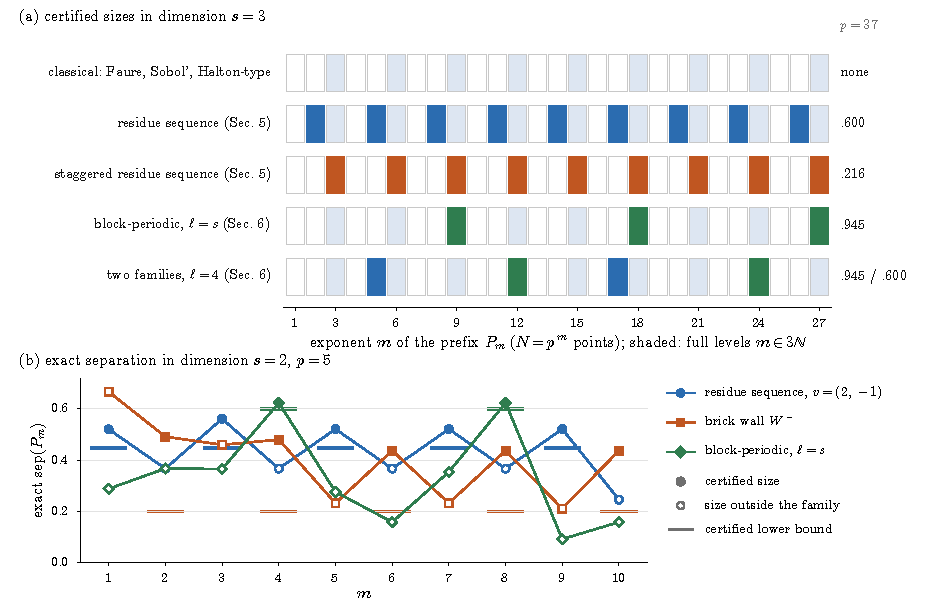
\includegraphics[width=0.9\linewidth]{fig_levels.pdf}
\caption{Level families. (a)~The exponents $m\le27$ at which each construction has a certified lower bound on $\sep{P_m}$ in dimension $s=3$ (filled; shaded columns are the full levels), with the certified constant at $p=37$: residue sequence, best check vector of Table~\ref{tab:residue} (Theorem~\ref{thm:residue}); staggered residue sequence with dyadic weights, $8/37$ (Corollary~\ref{cor:dyadic}); block-periodic residue sequence, $1-2/37$ (Theorem~\ref{thm:block}(b)); block period $\ell=4$ (Theorem~\ref{thm:blocktwo}): the design at $m\in12\N$ and skeleton relations at $m=5,17,29,\dots$ (blue). The classical sequences have no certified level; they fail along explicit sequences of levels (Section~\ref{sec:fail}). (b)~Exact $\sep{P_m}$, $m=1,\dots,10$, in dimension two over $\F_5$: the residue sequence with the Korobov vector $v=(2,-1)$ (certified $0.447$ at odd $m$), the brick wall $W^-$ (certified $0.2$ at even $m$, Theorem~\ref{thm:WF}) and the block-periodic sequence of Theorem~\ref{thm:block}(a) (certified $0.6$ at $m\in4\N$). Filled markers: sizes in the level family; bars: the certified bounds. Off its family a sequence is not controlled: the block-periodic sequence falls to $0.092$ at $m=9$ and the residue sequence to $0.246$ at $m=10$. Exact computations from the generator matrices.}
\label{fig:levels}
\end{figure}

\emph{What more is possible, and what is not.} Why not $s$ exact relations at every full level, which would put the design of the nets into every full level of one sequence? Within the scrambles of generalized Faure sequences, and for exact linear relations of bounded depth among the digits, this is impossible: a late enough range of $R+1$ consecutive levels carries at most $J+R+1$ independent relations of depth at most $J$, about one per level (Theorem~\ref{thm:count}, a residue-theorem argument at a single place). So all $s$ geometric digits can be designed on at most a fraction $1/s$ of the full levels, which the block-periodic sequences attain (Corollary~\ref{cor:layer}); the skeleton relations of the residue sequence and designed geometric digits share one count (Corollary~\ref{cor:density}); and no designed geometric digit fits at a full level next to skeleton relations (Corollary~\ref{cor:nodesign}). Section~\ref{sec:count} states the scope of each of these statements. To reach every full level with constants tending to $1$, Section~\ref{sec:antipode} uses certificates that are not exact relations: it keeps each carry response inside a fixed set of allowed values, a \emph{window}, by choosing the free digits of a self-similar scramble one at a time. Half a cell is, up to $1/p$, the only offset that is equally good for a forward step, a backward step and no step (Lemma~\ref{lem:antipode}); staggering one coordinate by half a cell against all the others gives $1-O(1/p)$ at every full level for large primes, in every dimension (Theorem~\ref{thm:A}). In a stated scope, windows and the skeleton relations of the residue sequence cannot be selected together (Proposition~\ref{prop:joint}).

\emph{Results.} All sequences of this paper are explicit linear scrambles of generalized Faure sequences, hence digital $(0,s)$-sequences, with star discrepancy $O((\log N)^s/N)$ \cite{Nie92}. Each comes with a lower bound on $\sep{P_m}=\delta(P_m)N^{1/s}$ at every $m$ of its level family and is therefore quasi-uniform. Table~\ref{tab:results} lists the results; the headlines are these.
\begin{enumerate}
\item \emph{The classical sequences fail} (Section~\ref{sec:fail}, Table~\ref{tab:negative}), with explicit close pairs.
\item \emph{A closed form in every dimension.} For every $s\ge2$ and every prime $p>2^s$ the residue sequence with a Korobov check vector is a quasi-uniform digital $(0,s)$-sequence with $\sep{P_{sK-1}}\ge(\rho-1)p^{-1/s}>1-2p^{-1/s}$ for every $K$ (Theorem~\ref{thm:residue}, Corollaries~\ref{cor:korobov} and~\ref{cor:residueQU}), and the staggered residue sequence has $\sep{P_{sK}}\ge(\lfloor p/2^{s-1}\rfloor-1)/p$ for every $K$ (Corollary~\ref{cor:dyadic}). With searched check vectors the constant of the residue sequence reaches $1.024$ in dimension two ($p=1009$) and $1.035$ in dimension three ($p=10007$) (Table~\ref{tab:residue}).
\item \emph{Separation $1-O(1/p)$ from small primes on, at every $s$-th full level.} The block-periodic residue sequences have $\sep{P_{s^2K}}\ge1-2/p$ for every prime $p\ge3$ ($s=2$) and $p\ge5$ ($s=3$), and $1-(a^*_s+1)/p$ in every dimension $s\ge4$ for $p\ge5a^*_s+4$; with a smaller diagonal of the design, $1-4/p$, $1-8/p$, $1-15/p$, $1-60/p$ for $s=4,\dots,7$ and every prime $p\ge11$, $23$, $37$, $191$ (Theorem~\ref{thm:block}; computer-assisted for these four).
\item \emph{Limits of exact relations} (Section~\ref{sec:count}): about one exact relation of bounded depth per level, in the scope stated there.
\item \emph{Every full level.} For every $s\ge3$ a closed form gives $\sep{P_{sK}}\ge1-C''_s/p$ for every prime $p\ge p_0(s)$ (Theorem~\ref{thm:A}), in dimension three $1-742/p$ for every prime $p\ge1.97\cdot10^7$ (Theorem~\ref{thm:A3}); in dimension two, $1-17/p$ for every prime $p>3677$ (Corollary~\ref{cor:HB17}).
\item \emph{Every base in small dimensions} (Theorem~\ref{thm:coverage}, which lists the level families). In dimension two every prime base is covered (base $3$ by Theorem~\ref{thm:block}(a) and, at every full level, by a computer-assisted bound); in base $2$ the sequence is a two-sided scramble of the Sobol' sequence with $\sep{P_{2K}}\ge0.3678$, which answers a question of Dick, Goda and Suzuki \cite[Section~4.2]{DGS2}: it is well-separated in their sense \cite[Def.~3.8]{DGS2} (Theorem~\ref{thm:B2}). In dimension three every prime base $p\ge3$ is covered, base $5$ at the sizes $5^{9K}$ only, and base $4$; in dimension four every prime $p\ge7$ and base $4$; in dimension five every prime $p\ge11$; in dimension six every prime $p\ge17$; in every dimension $s$ every prime $p>2^s$; and prime-power bases in dimensions two to five (Table~\ref{tab:primepower}).
\end{enumerate}

\begin{table}[t]
\centering
\footnotesize
\setlength{\tabcolsep}{2.3pt}
\caption{The main results: digital $(0,s)$-sequences in base $q$ with $\sep{P_m}\ge\LB$, the entry of the fourth column, for every $m$ in the stated level family, hence quasi-uniform; the fifth column is the resulting bound $\delta(P_{[N]})N^{1/s}\ge\cdot$ for every $N\ge2$ (Lemma~\ref{lem:prefix}). Form: \emph{closed}, explicit functions of $p$ (for the window constructions with any admissible choice of the free digits); \emph{table}, a finite certificate. Proof: \emph{proof${}^\star$}, the last step is one exact rational evaluation; \emph{c.a.}, computer-assisted (Section~\ref{sec:conventions}). $\rho=\lfloor p^{1/s}\rfloor$; $a^*_4=5$, $a^*_5=16$. First row: the closed form $(\rho-1)p^{-1/s}$ is proved; the values for searched check vectors $v$ are exact finite evaluations (c.a.). Not listed: the sequences of Theorem~\ref{thm:blocktwo} and Corollary~\ref{cor:gauss}, which are certified on two level families at once.}
\label{tab:results}
\begin{tabular}{@{}c>{\raggedright\arraybackslash}p{0.15\textwidth}l>{\raggedright\arraybackslash}p{0.25\textwidth}lll>{\raggedright\arraybackslash}p{0.13\textwidth}@{}}
\toprule
$s$ & base & levels $m$ & $\sep{P_m}\ge$ & all $N$ & form & proof & where\\
\midrule
$\ge2$ & prime $p>2^s$ & $s\N-1$ & $(\rho-1)p^{-1/s}>1-2p^{-1/s}$; searched $v$: $1.024$ ($s=2$), $1.035$ ($s=3$) & $\LB/p$ & closed & proof; c.a. & Thm.~\ref{thm:residue}, Cor.~\ref{cor:korobov}, Tab.~\ref{tab:residue}\\
$\ge2$ & prime $p>2^s$ & $s\N$ & $(\lfloor p/2^{s-1}\rfloor-1)/p$ & $\LB/p$ & closed & proof & Cor.~\ref{cor:dyadic}\\
$2$ & prime $p\ge3$ & $4\N$ & $1-2/p$ & $\LB/p^2$ & closed & proof & Thm.~\ref{thm:block}\\
$3$ & prime $p\ge5$ & $9\N$ & $1-2/p$ & $\LB/p^3$ & closed & proof & Thm.~\ref{thm:block}\\
$4$; $5$ & prime $p\ge11$; $23$ & $16\N$; $25\N$ & $1-4/p$; $1-8/p$ & $\LB/p^s$ & closed & c.a. & Thm.~\ref{thm:block}\\
$6$; $7$ & prime $p\ge37$; $191$ & $36\N$; $49\N$ & $1-15/p$; $1-60/p$ & $\LB/p^s$ & closed & c.a. & Thm.~\ref{thm:block}\\
$\ge4$ & prime $p\ge5a^*_s+4$ & $s^2\N$ & $1-(a^*_s+1)/p$ & $\LB/p^s$ & closed & proof & Thm.~\ref{thm:block}\\
$\ge3$ & prime $p\ge p_0(s)$ & $s\N$ & $1-C''_s/p$ & $\LB/p$ & closed & proof & Thm.~\ref{thm:A}\\
$3$ & prime $p\ge1.97\cdot10^7$ & $3\N$ & $1-742/p$ & $\LB/p$ & closed & proof${}^\star$ & Thm.~\ref{thm:A3}\\
$2$ & prime $p>3677$ & $2\N$ & $1-17/p$ & $\LB/p$ & closed & proof${}+{}$c.a. & Cor.~\ref{cor:HB17}\\
$2$ & $2$ & $2\N$ & $0.3678$ & $\LB/2$ & closed & c.a. & Thm.~\ref{thm:B2}\\
$3$ & $3$; $4$ & $3\N$ & $0.05598$; $0.11293$ & $\LB/q$ & closed & c.a. & Thms.~\ref{thm:S3}, \ref{thm:K4}\\
$3$ & $7$ & $3\N$ & $1/7$ & $\LB/7$ & table & c.a. & Thm.~\ref{thm:p7}\\
$4$ & $4$ & $4\N$ & $0.03013$ & $\LB/4$ & closed & c.a. & Thm.~\ref{thm:S4}\\
$2$--$5$ & $\F_8,\dots,\F_{169}$ (Tab.~\ref{tab:primepower}) & $s\N$ & Table~\ref{tab:primepower} & $\LB/q$ & closed & c.a. & Prop.~\ref{prop:primepower}\\
\bottomrule
\end{tabular}
\end{table}

\emph{Small bases and practice.} In the bases $2$, $3$ and $4$ neither residues nor windows give anything at every full level. There we choose frames whose local roots are lacunary series, such as $\sum_kx^{2^k}$, so that the responses are computed by a small finite automaton and the bound at every level is one finite minimum (Section~\ref{sec:frames}). Section~\ref{sec:frames} also reads the staggered residue sequence over prime-power fields and collects the coverage by dimension. In practice (Section~\ref{sec:practice}) the residue sequences are generated like any digital sequence, from closed-form matrices, and they stay certified under digital shifts (Lemma~\ref{lem:shift}). In dimension three their smallest $\sep{P_{[N]}}$ over $64\le N\le2^{23}$ is $0.235$ to $0.267$ at $p=13$, $17$, $23$, $31$: six to eighteen times the Owen-scrambled Sobol' sequence and $1.7$ to $1.9$ times the best plain Faure sequence (Figure~\ref{fig:evidence}, Table~\ref{tab:practice}).

\emph{Scope.} Each bound holds at the sizes of its level family; between them Lemma~\ref{lem:prefix} loses the factor $q^{-\Delta_{\Lev}/s}$ (in Figure~\ref{fig:evidence}, $0.636$ at the certified size against $0.020$ for all $N$, with an observed minimum of $0.267$). The bounds are lower bounds, often loose at small primes (for $s=3$, $p=11$ the residue sequence has the certified $0.449$ against the exact $0.7686$ and $0.6144$ at $m=2$ and $m=5$), and at its first full level the Faure sequence is better than ours. The constants $1-O(1/p)$ at every full level concern large primes ($p>3677$ in dimension two, $p\ge1.97\cdot10^7$ in dimension three, $p_0(4)\le1.44\cdot10^{16}$); at every $s$-th full level they hold from small primes on. Base $5$ in dimension three at every full level, the primes $s\le p<2^s$ for $s\ge4$ at every full level (and, outside the ranges above, at any level family), and the prime-power bases beyond Proposition~\ref{prop:primepower} are open, and we measured separation, not integration error. These caveats are not repeated below.

\emph{Related work.} Quasi-uniformity of quasi-Monte Carlo point sets was studied systematically in \cite{DGLPS1,DGS2}. Sobol' and Shukhman suggested from numerical experiments that the Sobol' sequence keeps its points at distance of order $N^{-1/s}$ \cite{SS07}; Goda disproved this for $s=2$ \cite{Goda23}, and Corollary~\ref{cor:sobol} disproves it in every dimension $s\ge2$. The negative results before this paper are those of Table~\ref{tab:negative}: the two-dimensional Sobol' sequence \cite{Goda23}, whose mesh ratio grows at least like $N^{1/4}$ \cite{Suz25}, the Faure sequence of dimension equal to its base \cite{DGS2}, the Halton sequences and three families of Halton-type sequences \cite{GHS26}, and Owen-scrambled $(t,s)$-sequences, almost surely \cite{Suz26}; Suzuki also shows that random linear scrambles of binary digital nets with fixed $t$ have mesh ratio $O_P(\log N)$ under a uniform coincidence condition, which holds for instance for the prefixes of Sobol' sequences \cite[Thm.~5.5, Lem.~4.10]{Suz26}. Without digital structure, quasi-uniform sequences exist in every dimension: Kronecker sequences with badly approximable parameters \cite[Thm.~3.9]{DGLPS1}, with discrepancy $O(N^{-1+\varepsilon})$ for algebraic parameters \cite[Section~3.3]{DGLPS1}, and greedy farthest-point sequences \cite{PZ23,GX26}, without a discrepancy guarantee; neither is a $(t,s)$-sequence. Sakai and Goda \cite{SG26} select quasi-uniform rank-1 and Korobov lattice point sets, one for each $N$. Goda \cite{Goda26} constructs Kronecker sequences whose two-dimensional projections are quasi-uniform for every $N$, and nested lattices with this property at $N=p^m$. Among digital nets, the Larcher--Pillichshammer nets are quasi-uniform \cite{LP01,DGS2}, and \cite{Gru26geo} gives quasi-uniform digital $(0,m,s)$-nets in every dimension with separation $1-O(1/q)$; %
in both cases there is a separate net for each $m$. Generalized Faure sequences and their scrambles are classical \cite{Fau82,Nie87,Tez93,Tez95,Owe95,Mat98}; Tezuka's generalized Niederreiter sequences \cite{Tez93} define generator rows by Laurent coefficients. Mayor and Niederreiter \cite{MN07} construct digital sequences from differentials of function fields; in genus~$0$ their construction contains every scramble of a frame, in the residue form of Lemma~\ref{lem:resform}, and so every sequence of this paper. Niederreiter and \"Ozbudak \cite{NO07} read all coordinates as residues of one differential and use the residue theorem over all places for a duality. In these works the aim is the quality parameter $t$. Choosing the scramble so that the residue theorem ties one digit of every coordinate together with constant coefficients at every level of a level family, and using this for the separation, was not found in the literature we searched. In computer graphics, separation is an explicit design goal. Gr\"unschlo{\ss}, Hanika, Schwede and Keller \cite{GHSK08} and Gr\"unschlo{\ss} and Keller \cite{GK09} construct $(0,m,2)$- and $(0,m,3)$-nets with large minimum distance by search and by permutations, a new net for each $m$. Ahmed and Wonka \cite{AW21} optimise dyadic nets and prove $\delta\sqrt N=1/\sqrt2$ for a Gray-code net of each size $4^k$; these nets are not nested. The progressive multi-jittered sequences of Christensen, Kensler and Kilpatrick \cite{CKK18} and the stochastic $(t,s)$-sequences of Helmer, Christensen and Kensler \cite{HCK21} are built by randomised best-candidate choices; their separation is empirical. Bonneel, Coeurjolly and Ostromoukhov \cite{BCO26} construct $(0,s)$-sequences from Artin--Schreier polynomials; their subject is the quality parameter $t$, not separation, and their polynomials define Sobol'-type sequences, whereas our Artin--Schreier frames are a choice of places with lacunary local roots (Section~\ref{sec:frames}).

This paper keeps the frames, the cells, the geometric digits, the lattice image and the designs of \cite{Gru26geo}, and answers the question that paper leaves open: whether one fixed scramble can serve all scales. %
The new ingredients are the failure theorem for polynomial bases, the residue theorem as a design tool for the separation, the count of exact relations, and the windows.

\emph{Organisation.} Section~\ref{sec:prelim} fixes the objects, the level families and the conventions. Section~\ref{sec:fail} proves that the classical sequences fail. Section~\ref{sec:law} describes the position of a point inside its cell, the residue form of a scramble and the self-similar scrambles. Sections~\ref{sec:residue} and~\ref{sec:block} construct the residue and block-periodic residue sequences, Section~\ref{sec:count} counts exact relations, and Section~\ref{sec:antipode} certifies every full level with windows. Section~\ref{sec:frames} treats the small bases, prime powers and the coverage by dimension, Section~\ref{sec:practice} implementation, practice and randomisation, and Section~\ref{sec:open} open problems. The appendices hold secondary proofs, the base-$7$ bound in dimension three, the computer-assisted parts with the archive and the Lean status, and the staggered windows at a finite prime with their data.

%
\section{Digital Sequences, Frames and Separation}\label{sec:prelim}
This section fixes the objects and the conventions. Everything here is classical except for the normalisation of the separation constant and the form of the prefix lemma (Lemma~\ref{lem:prefix}): a bound at the prefixes of one family of sizes, with bounded gaps between consecutive sizes, gives a bound for every number of points.

\subsection{Digital Nets and Sequences}
Let $q=p^r$ be a prime power and $s\ge1$. Digits live in $\F_q$ and are read through a fixed bijection $\enc\colon\F_q\to\{0,\dots,q-1\}$ with $\enc(0)=0$. For prime $q$ it is the identity on $\{0,\dots,p-1\}$. For a prime power we use the \emph{natural identification} of Niederreiter \cite{Nie92}: fix a basis of $\F_q$ over $\F_p$ that contains~$1$, and read an element with coordinates $(x_0,\dots,x_{r-1})\in\{0,\dots,p-1\}^r$ as the integer $\sum_ix_ip^i$. For $\F_4=\{0,1,\omega,\omega^2\}$ with the basis $(1,\omega)$ this is $0,1,\omega,\omega^2\mapsto0,1,2,3$. We write $\bar y:=\enc^{-1}(q-1)$ for the top digit ($\bar y=-1$ for prime $q$). A point set lives on the torus $[0,1)^s=\R^s/\Z^s$.

An \emph{elementary box} in base~$q$ is a product $\prod_cI_c$ in which $I_c$ is one of the $q^{d_c}$ intervals $[iq^{-d_c},(i+1)q^{-d_c})$, $0\le i<q^{d_c}$, for integers $d_c\ge0$. A set of $q^m$ points is a \emph{$(t,m,s)$-net in base~$q$} if every elementary box of volume $q^{t-m}$ contains exactly $q^t$ points. An infinite sequence of points in $[0,1)^s$ is a \emph{$(t,s)$-sequence in base~$q$} if for all $k\ge0$ and $m\ge t$ its points number $kq^m,\dots,(k+1)q^m-1$ form a $(t,m,s)$-net \cite{Nie87,Nie92,DP10}. The letter $t$ always denotes this quality parameter. A $(t,s)$-sequence has star discrepancy $O((\log N)^s/N)$ \cite{Nie92}, so every sequence of this paper is a low-discrepancy sequence.

\emph{The index.} We never write the index of a point as an integer variable. The point is labelled by its \emph{index polynomial} $V(z)=\sum_kV_kz^k\in\F_q[z]$, whose coefficients $V_k\in\F_q$ are the \emph{index digits} ($V_0$ least significant). The integer index of the point is
\[
\ind{V}=\sum_k\enc(V_k)\,q^k,
\]
so the $N$-th point of the sequence, counted from $0$, is the point whose index polynomial has $\ind{V}=N$. A \emph{digital sequence} over $\F_q$ is given by $s$ generator matrices $C_0,\dots,C_{s-1}\in\F_q^{\N_0\times\N_0}$; digit~$n$ of coordinate~$c$ of the point $y(V)$ is
\[
y_{c,n}(V)=\sum_kC_c[n][k]\,V_k,\qquad y_c(V)=\sum_{n\ge0}\enc\bigl(y_{c,n}(V)\bigr)\,q^{-n-1}.
\]
Rows are output digits (row~$0$ is the most significant digit) and columns are index digits. If the digits of $y_c(V)$ are eventually $\bar y$, the point lies on the upper boundary of the elementary box named by its digits; as usual \cite[Section~4.1]{Nie92} we assign it to that box, and the separation bounds below allow this (the jitter in (\ref{eq:cellunits}) may equal $q^{-j}$). We write $Y_c(x)=\sum_ny_{c,n}x^n$ for the digit series of coordinate~$c$. Coordinates are numbered $c=0,\dots,s-1$.

The \emph{prefix} $P_m=\{y(V):\deg V<m\}$ consists of the first $q^m$ points, and $P_{[N]}=\{y(V):\ind{V}<N\}$ of the first $N$ points for general $N$. By Niederreiter's criterion \cite[Thm.~6.1]{Nie87} (the box criterion of \cite{Gru26geo}%
), $P_m$ is a $(0,m,s)$-net if and only if for every $d=(d_0,\dots,d_{s-1})$ with $\sum_cd_c=m$ the \emph{box matrix}, formed by the first $d_c$ rows of every $C_c$ restricted to the columns $0,\dots,m-1$, is invertible. The points numbered $kq^m,\dots,(k+1)q^m-1$ form a digital shift of $P_m$ (the index digits from $m$ on are fixed), and a digital shift maps every elementary box onto one of the same shape. Hence a digital sequence is a $(t,s)$-sequence if and only if every prefix $P_m$ is a $(t,m,s)$-net.

The prefixes $P_{sK}$ are the \emph{full levels}. At level~$K$ the prefix has $N=q^{sK}$ points, and the elementary boxes with $K$ digits in every coordinate, the \emph{cells}, have side $q^{-K}=N^{-1/s}$; a $(0,sK,s)$-net has exactly one point in each cell. (The companion paper \cite{Gru26geo} calls the level $k$.) Not every result of this paper is about full levels: each one names the set of exponents~$m$ at which it bounds $P_m$ (Section~\ref{sec:levels}).

\subsection{Frames and Scrambles}
All sequences in this paper are scrambles of one classical family, the generalized Faure sequences of Faure \cite{Fau82}, Niederreiter \cite{Nie87} and Tezuka \cite{Tez93,Tez95}. As in \cite{Gru26geo} we describe them by \emph{places} on the projective line over $\F_q$. Fix distinct elements $a_0,\dots,a_{s-1}\in\F_q$ (so $s\le q$), the places of the coordinates. Coordinate $c$ of the unscrambled point reads the Taylor coefficients of the index polynomial at $a_c$:
\[
y_{c,n}(V)=[(z-a_c)^n]\,V,\qquad\text{i.e.}\qquad C_c=\Pas_{a_c},\quad \Pas_a[n][k]=\binom kn a^{k-n}.
\]
The index itself is read at the place $\infty$: the prefix $P_m$ is the set of polynomials with a pole of order less than $m$ at $\infty$. We call $(a_0,\dots,a_{s-1};\infty)$ a \emph{frame}. For prime $q=p$ and the \emph{Faure places} $0,1,\dots,s-1$ this is the Faure sequence $(I,\Pas,\Pas^2,\dots,\Pas^{s-1})$, since $\Pas_a=\Pas_1^a$; in dimension two it is $(I,\Pas)$, which for $q=2$ is the two-dimensional Sobol' sequence \cite{Sob67}. Up to a scramble, the frame sequence is the Niederreiter sequence with the linear base polynomials $z-a_c$ \cite{Nie87}. For prime $q$ it is also exactly the Halton-type sequence of Goda, Hofer and Suzuki \cite[Def.~2]{GHS26} with the monic linear bases $z-a_c$: the $(z-a_c)$-adic digits of the index polynomial are its Taylor coefficients at $a_c$, and their index and digit conventions coincide with ours. For $s\ge2$ no such sequence is quasi-uniform (Section~\ref{sec:fail}).

In words: read the digits of the index as a polynomial $V$; coordinate $c$ is the Taylor expansion of $V$ around its own point $a_c$. For example, let $q=3$ and $V=2+z$ (integer index $5=2+1\cdot3$). At $a=0$ the Taylor digits are $(2,1)$; at $a=1$, $V=0+1\cdot(z-1)$ in $\F_3$, so the digits are $(0,1)$. A polynomial of degree less than $2$ is determined by $(V(0),V(1))$, that is, by its cell: this is the net property for $s=2$ and one digit per coordinate, and Lemma~\ref{lem:t0} below is the same statement for every $s$ and every number of digits.

A Taylor coefficient is a residue: $[(z-a)^n]V=\Res_a\bigl(V\,(z-a)^{-n-1}dz\bigr)$, where $\Res_a(F\,dz)$ denotes the coefficient of $(z-a)^{-1}$ in the expansion of $F$ in powers of $z-a$. Section~\ref{sec:law} uses this to write every scramble, and Sections~\ref{sec:residue}--\ref{sec:count} use it to design them.

A \emph{scramble} of coordinate $c$ is an infinite lower-triangular matrix $L_c$ with nonzero diagonal, fixed once and for all (independent of $m$). The scrambled sequence has the generator matrices $C_c=L_c\Pas_{a_c}$: digit $n$ of the scrambled coordinate is a linear combination of the unscrambled digits $0,\dots,n$, with a nonzero coefficient on digit~$n$. Dick, Goda and Suzuki, and Goda, Hofer and Suzuki, number the coordinates from $1$, so $(L_1,L_2\Pas)$ in the notation of \cite{DGS2} is $(L_0,L_1\Pas_1)$ here.

\begin{lemma}[Frames have $t=0$]\label{lem:t0}
For distinct places $a_0,\dots,a_{s-1}\in\F_q$ and arbitrary scrambles $L_0,\dots,L_{s-1}$, the digital sequence with generator matrices $C_c=L_c\Pas_{a_c}$ is a $(0,s)$-sequence in base~$q$.
\end{lemma}

\begin{proof}
Let $m\ge1$ and $\sum_cd_c=m$. For the unscrambled frame, the first $d_c$ digits of coordinate $c$ are the coefficients of $V\bmod(z-a_c)^{d_c}$ in the basis $(z-a_c)^n$. By the Chinese remainder theorem the map $V\mapsto(V\bmod(z-a_c)^{d_c})_c$ is a bijection from the polynomials of degree less than $m$ onto $\prod_c\F_q[z]/((z-a_c)^{d_c})$: both sides have $q^m$ elements, and a polynomial of degree less than $m$ divisible by $\prod_c(z-a_c)^{d_c}$ is zero. So every box matrix is invertible. A lower-triangular $L_c$ replaces the first $d_c$ rows of $C_c$ by an invertible combination of themselves, so every box minor is multiplied by $\prod_c\det L_{c,[d_c]}\ne0$, where $L_{c,[d]}$ is the leading $d\times d$ block (the scrambling identity of \cite{Gru26geo}%
). Every prefix is therefore a $(0,m,s)$-net.
\end{proof}

That scrambling preserves $t$ is classical: for nested random scrambles it is due to Owen \cite{Owe95}, and for lower-triangular linear scrambles it underlies the generalized Faure sequences of Tezuka \cite{Tez95} and Matou\v{s}ek's linear scrambling \cite{Mat98}. So $t=0$ comes for free; what the scramble changes, and what this paper is about, is the position of each point inside its cell.

\subsection{Separation and Quasi-Uniformity}
For $\mathbf y,\mathbf y'\in[0,1)^s$ let $\|\mathbf y-\mathbf y'\|_{\mathrm T}=\min_{\mathbf k\in\Z^s}\|\mathbf y-\mathbf y'+\mathbf k\|$ be the toroidal Euclidean distance. For a finite point set $P$ with $N\ge2$ points, the \emph{separation} is
\[
\delta(P)=\min_{\mathbf y\ne\mathbf y'\in P}\|\mathbf y-\mathbf y'\|_{\mathrm T},\qquad\text{and}\qquad \sep{P}=\delta(P)\,N^{1/s}
\]
is its \emph{separation constant}. A $(0,sK,s)$-net has one point in each cell of side $N^{-1/s}$, so $\sep{P}$ measures the separation in cell units; $\sep{P}=1$ for the grid $q^{-K}\Z^s$.

The \emph{covering radius} is $h(P)=\sup_{\mathbf y\in[0,1]^s}\min_{\mathbf y'\in P}\|\mathbf y-\mathbf y'\|$, and $h(P)/\delta(P)$ is the \emph{mesh ratio}. A sequence is \emph{quasi-uniform} if the mesh ratio $h(P_{[N]})/\delta(P_{[N]})$ is bounded over all $N\ge2$ \cite{DGLPS1,DGS2}. Since $h(P)\gtrsim N^{-1/s}$ and $\delta(P)\lesssim N^{-1/s}$ for every $N$-point set, this is the same as $h(P_{[N]})\asymp N^{-1/s}$ and $\delta(P_{[N]})\asymp N^{-1/s}$. We state mesh ratios as $h/\delta$; the convention of \cite{DGS2} divides by the separation radius $\delta/2$ and gives twice our value.

\emph{Which distance.} The toroidal distance never exceeds the Euclidean distance in the cube. Our lower bounds on $\delta$ are toroidal, so they hold for the Euclidean separation of \cite{DGLPS1,DGS2,GHS26} as well. Our upper bounds on $\delta$ (the close pairs of Section~\ref{sec:fail}) bound the Euclidean distance in the cube, so they bound the toroidal separation too. Our bounds on $h$ are for the Euclidean distance in the cube. So every statement transfers to both conventions in the direction in which it is used.

\subsection{Level Families}\label{sec:levels}
For a $(0,s)$-sequence the covering radius is never the problem: the prefixes are nets at every scale. The problem is the separation, and it suffices to control it along one family of prefixes. The general principle, that quasi-uniformity along a subsequence of sizes with bounded ratios implies quasi-uniformity along all $N$, is \cite[Lemma~1.3]{DGLPS1}; we give the toroidal version with explicit constants, for the families of prefixes that occur in this paper.

A \emph{level family} is an infinite set $\Lev\subseteq\N=\{1,2,\dots\}$ of exponents $m$, namely those at which a result certifies a bound on $\sep{P_m}$. Its \emph{largest gap} is
\[
\Delta_{\Lev}:=\max\bigl(\min\Lev,\ \sup\{m'-m:\ m<m'\text{ consecutive elements of }\Lev\}\bigr).
\]
The families of this paper are $\Lev=s\N$ (all full levels, $\Delta_{\Lev}=s$), $\Lev=s\N-1=\{s-1,2s-1,\dots\}$ ($\Delta_{\Lev}=s$), $\Lev=s^2\N$ ($\Delta_{\Lev}=s^2$), and unions of residue classes of these (Section~\ref{sec:block}).

\begin{lemma}[Prefix lemma]\label{lem:prefix}
Let $(y(V))$ be a $(0,s)$-sequence in base $q$ and $\Lev$ a level family with $\Delta:=\Delta_{\Lev}<\infty$. Suppose that $\sep{P_m}\ge\LB$ for every $m\in\Lev$, with $\LB>0$. Then for every $N\ge2$
\[
\delta(P_{[N]})\ge\LB\,q^{-\Delta/s}\,N^{-1/s},\qquad h(P_{[N]})\le\sqrt s\,q\,N^{-1/s},\qquad \frac{h(P_{[N]})}{\delta(P_{[N]})}\le\frac{\sqrt s\,q^{1+\Delta/s}}{\LB}.
\]
In particular the sequence is quasi-uniform.
\end{lemma}

\begin{proof}
\emph{Separation.} Let $N\ge2$ and let $m'$ be the least element of $\Lev$ with $q^{m'}\ge N$. Then $P_{[N]}\subseteq P_{m'}$, and a subset has at least the separation of the whole set, so $\delta(P_{[N]})\ge\delta(P_{m'})\ge\LB\,q^{-m'/s}$. It remains to show $q^{m'}\le q^{\Delta}N$. If $m'=\min\Lev$, then $q^{m'}\le q^{\Delta}\le q^{\Delta}N$. Otherwise $m'$ has a predecessor $m''$ in $\Lev$; by the choice of $m'$, $q^{m''}<N$, and $m'-m''\le\Delta$, so $q^{m'}\le q^{\Delta}q^{m''}<q^{\Delta}N$.

\emph{Covering.} Let $m\ge0$ with $q^m\le N<q^{m+1}$, and write $m=sK+j$ with $0\le j<s$. The first $q^m$ points form the prefix $P_m\subseteq P_{[N]}$, which is a $(0,m,s)$-net. Split the cube into the elementary boxes with $K+1$ digits in the first $j$ coordinates and $K$ digits in the others. Each has volume $q^{-m}$, so it contains a point of $P_m$, and its diameter is at most $\sqrt s\,q^{-K}$. Every point of $[0,1]^s$ lies in the closure of one of these boxes, so $h(P_{[N]})\le\sqrt s\,q^{-K}$. Finally $q^{-K}=q^{(j-m)/s}<q^{(j+1)/s}N^{-1/s}\le q\,N^{-1/s}$, since $j+1\le s$.

The bound on the mesh ratio is the quotient of the two bounds.
\end{proof}

\begin{remark}[The cases used]\label{rem:prefixcases}
For $\Lev=s\N$ and $\Lev=s\N-1$ the factor is $q^{-\Delta/s}=1/q$: $\delta(P_{[N]})\ge(\LB/q)N^{-1/s}$. For $\Lev=s^2\N$ it is $q^{-s}$. For $\Lev=s\N$ comparing the two intermediate bounds directly gives the sharper mesh ratio $h/\delta\le\sqrt s\,q/\LB$: if $q^{sK}\le N<q^{s(K+1)}$, the covering argument gives $h\le\sqrt s\,q^{-K}$ and the separation argument $\delta\ge\LB\,q^{-K-1}$ (for $K=0$, $h\le\sqrt s$ and $\delta\ge\LB/q$).
\end{remark}

The lemma loses the factor $q^{-\Delta/s}$ only at the prefixes between two elements of $\Lev$: for consecutive $m''<m<m'$ in $\Lev$ the separation argument gives $\sep{P_m}\ge\LB\,q^{(m-m')/s}$. A construction certified at a denser family therefore has the better bound for all $N$, even when its constant at the certified levels is smaller (Sections~\ref{sec:block} and~\ref{sec:count}).

\subsection{Conventions}\label{sec:conventions}
Every result names its level family: the exponents $m$ at which it bounds $\sep{P_m}$, for every element of the family at once. The bound for all $N$ then follows from Lemma~\ref{lem:prefix}.

Every result has a written proof. Some proofs end in an exact finite computation: a minimum over an explicitly enumerated finite set, or explicit integer hypotheses checked at each prime of a finite range. We call such a proof \emph{computer-assisted} (c.a.) and state its scope with the result. A proof whose last step is one exact rational evaluation is marked \emph{proof${}^\star$}; the threshold $p_0(s)$ of Section~\ref{sec:antipode} is the infimum of explicit monotone conditions, and an upper estimate of it is certified in this way. Searches only find parameters (multipliers, check vectors, window systems, tables), whose properties are then proved or checked; a value found by a search is a lower bound on an optimum, never a claim of optimality. Exact separations quoted for figures and tables are illustrations. No proof uses a search or an illustration. A statement that a construction fails, or that a kind of certificate cannot do better, is always made with its exact scope (which sequences, which scrambles, which kind of certificate); a finite search is never used as evidence that something does not exist. Appendix~\ref{app:cert} lists the data, the independent re-verification and the parts that are in addition verified in Lean. Table~\ref{tab:glossary} lists the main symbols and terms.

%
\begin{table}[!tp]
\centering
\footnotesize
\caption{Notation and terms at a glance. Terms marked \cite{Gru26geo} are used in the sense of the companion paper on nets.}
\label{tab:glossary}
\renewcommand{\arraystretch}{0.9}\setlength{\tabcolsep}{3pt}
\begin{tabular}{@{}>{\raggedright\arraybackslash}p{0.24\textwidth}>{\raggedright\arraybackslash}p{0.61\textwidth}l@{}}
\toprule
symbol or term & meaning & defined in\\
\midrule
$q$, $p$, $s$ & base (prime power $q=p^r$), its characteristic, dimension & \S\ref{sec:prelim}\\
$V$, $\ind{V}$ & index polynomial of a point; its integer index & \S\ref{sec:prelim}\\
$P_m$, $P_{[N]}$ & first $q^m$ points, first $N$ points & \S\ref{sec:prelim}\\
full level, cell & prefix $P_{sK}$; elementary cube of side $q^{-K}$ & \S\ref{sec:prelim}\\
level family $\Lev$, $\Delta_{\Lev}$ & the exponents $m$ with a certified bound on $\sep{P_m}$; its largest gap & \S\ref{sec:levels}\\
$\sep{P}=\delta(P)N^{1/s}$ & toroidal separation in cell units ($1$ for the grid) & \S\ref{sec:prelim}\\
natural identification & digits of $\F_q$ read as integers through base-$p$ coordinates & \S\ref{sec:prelim}\\
frame, places $a_c$, $\Pas_a$ & coordinate $c$ reads the Taylor digits of $V$ at $a_c$; Pascal matrix & \S\ref{sec:prelim}\\
scramble $L_c$ & lower-triangular, nonzero diagonal, fixed for all prefixes & \S\ref{sec:prelim}\\
$b_c$-adic coordinate & its first $e_cQ$ digits depend only on $V\bmod b_c^Q$ & \S\ref{sec:fail}\\
radical inverse, digit map $\pi_c$ & digit block $Q$ is $\pi_c$ of the $Q$-th $b_c$-adic digit of $V$ & \S\ref{sec:fail}\\
Halton-type sequence & coordinate $c$ reads the $b_c$-adic digits of $V$; pairwise coprime $b_c\in\F_p[z]$ \cite{GHS26} & \S\ref{sec:fail}\\
geometric digit(s) $r_c$, $R_c$; layer & first digit(s) of coordinate $c$ below the cell; layer: their change $D(1)$ under a carry-free step & (\ref{eq:cellunits})\\
lattice image, jitter $\varepsilon_c$ & $n+\enc(R)/q^j$; the contribution of the deeper digits ($\le q^{-j}$) & (\ref{eq:cellunits})\\
offset map & linear map from the cell digits to the geometric digits of $P_{sK}$ & \S\ref{sec:law}\\
carry length $l$, carry depth & cell digits changed by a step; coefficient index from the finest digit & \S\ref{sec:law}\\
carry response $D_i(l)$ & change of digit $K+i$ under a carry of length $l$ in one coordinate & \S\ref{sec:law}\\
own, cross response & $O^{(l)}_c$: moving coordinate; $X^{(l)}_{c\leftarrow c'}$: coordinate $c$ when $c'$ moves & \S\ref{sec:law}\\
constant response & a response that does not depend on the carry length & \S\ref{sec:dislocations}\\
slip planes & hyperplanes where a geometric digit wraps around modulo $q$ & \S\ref{sec:dislocations}\\
jump of depth $l$ & change of the lattice image across a boundary of carry length $l\ge2$ & \S\ref{sec:dislocations}\\
uniformizer $w$, local root $z_c$ & $w=\prod_c(z-a_c)$; the root of $w(Z)=x$ at $a_c$ & (\ref{eq:roots})\\
self-similar scramble, $\theta$, $g_c$ & one multiplier series per coordinate; scale; multipliers & Def.~\ref{def:selfsim}\\
$\Res_a$, principal part & coefficient of $(z-a)^{-1}dz$; the polar terms at $a$ & \S\ref{sec:prelim}, Lem.~\ref{lem:resform}\\
local multiplier $\varphi_c$ & unit series in $z-a_c$; $y_{c,n}=\Res_{a_c}(V\varphi_c(\theta/w)^{n+1}dz)$ & Lem.~\ref{lem:resform}\\
$f_j$, $\LB_j$ & guaranteed gap in one coordinate; digit relaxation with $j$ digits & Lem.~\ref{lem:cert}\\
exact digit relation & linear identity among the digits of a prefix, of bounded depth & Def.~\ref{def:exactrel}\\
depth $J$; admissible range & relation of top index $T$ uses the digits $T-J,\dots,T$; levels $[K_0,K_0+R]$ of Thm.~\ref{thm:count} & Def.~\ref{def:exactrel}, \S\ref{sec:countthm}\\
level-independent relation & exact relation with the same coefficients at every level & Prop.~\ref{prop:onerel}\\
skeleton coordinate, digit & at $P_{sK-1}$: a coordinate with one cell digit fewer; its next digit & \S\ref{sec:residue}\\
skeleton relation, fine cell & $\sum_cv_cy_{c,K-1}=0$ on $P_{sK-1}$; cube of side $q^{-K}$ at $P_{sK-1}$ & \S\ref{sec:residue}\\
check vector $v$; $\Lambda_v$; $\ljit$ & $\Lambda_v=\{b\in\Z^s:v\cdot b\equiv0\bmod p\}$; $\ljit(\Lambda)=\min_{b\ne0}\|(|b|-1)_+\|_2$ & \S\ref{sec:residue}\\
residue sequence $\Rv_v$ & every coordinate reads the differential $V\,dz$ at its place & Def.~\ref{def:residue}\\
staggered res.\ sequence $\Rstar_v$, $\cstar$ & geometric digit of $\cstar$ = rank-1 lattice rule in the finest cell digits & Def.~\ref{def:residuestar}\\
$\cabs{x}$ & centred absolute value of $x\in\F_p$, in $[0,p/2]$ & \S\ref{sec:brickwall}\\
brick wall $W^-$ & $\Rstar_v$ for $s=2$: heights staggered by half a cell between columns & Def.~\ref{def:WF}\\
inclusion bound & bound on $\sep{P_{sK}}$ from $P_{sK}\subset P_{s(K+1)-1}$ & Rem.~\ref{rem:residuefull}\\
design, reachable & matrices $F_n$: geometric digits from the last cell levels \cite{Gru26geo} & \S\ref{sec:block}\\
block-periodic residue seq.\ & local multipliers repeat with period $\ell$ in the row index & Def.~\ref{def:block}\\
free series $\psi_c$; cross $\kappa_{c\leftarrow c'}$ & what a self-similar scramble leaves free; $\kappa_{c\leftarrow c'}=-X^{(1)}_{c\leftarrow c'}$ & Prop.~\ref{prop:LI}\\
window $W$, $\LB(W)$ & set of values a response may take; the bound given by the windows & Prop.~\ref{prop:steer}\\
covering condition & every line of the depth direction meets the window & Prop.~\ref{prop:steer}\\
selection rule, history & picks an admissible free digit at each depth; the digits chosen before & Prop.~\ref{prop:steer}\\
correction terms $\chi_{c,d}$, $\Psi_c$ & deeper digits in a corrected skeleton relation; their partial sums & Lem.~\ref{lem:corrS}\\
staggered windows, $\half$ & staggered coordinate offset by half a cell; $\half=(p+1)/2\in\F_p$ & \S\ref{sec:antipode}\\
first-order deficit & the constant $C$ in a bound $1-C/p$ \cite{Gru26geo} & \S\ref{sec:antipode}\\
$p_0(s)$ & threshold of the staggered rule & \S\ref{sec:antipode}\\
proof${}^\star$, c.a. & last step one exact rational evaluation; computer-assisted & \S\ref{sec:conventions}\\
\bottomrule
\end{tabular}
\end{table}


%
%
%
%
%
%
\section{Why the Classical Sequences Fail}\label{sec:fail}
The classical low-discrepancy sequences of Halton, Faure, Sobol' and Niederreiter are built from polynomial bases. Each coordinate reads the index polynomial in its own base $b_c(z)$, one block of digits at a time, like a radical inverse. Their prefixes are nets at every scale, so their covering radius is always of the right order $N^{-1/s}$. Dick, Goda and Suzuki asked for quasi-uniform digital sequences \cite{DGS2}, and Goda, Hofer and Suzuki asked whether any Halton-type sequence is \cite{GHS26}. For the classical sequences of all four kinds the answer is no, and the reason is one picture.

Take two indices whose difference is a carry in the last digits of one coordinate. In base $p$ the digits $0.a(p-1)\cdots(p-1)$ of one point become $0.(a+1)0\cdots0$ for the other: the two points sit on either side of a cell boundary, one unit of the last digit apart. If the same index difference is divisible by a high power of every other base, then it does not change the leading digits of any other coordinate. The two points are close in every coordinate at once, much closer than $N^{-1/s}$ (Figure~\ref{fig:carry}). For polynomial bases such differences exist at infinitely many sizes, because a run of ones in one base is divisible by high powers of all the other bases (Theorem~\ref{thm:nonqu}).

This section proves this for every digital sequence in polynomial bases with one coordinate a radical inverse (Theorem~\ref{thm:nonqu}), derives the classical cases (Halton-type, Faure, Niederreiter and Sobol' sequences), and shows which scrambles do not help: as long as one coordinate is still a radical inverse, up to a scalar, the sequence is not quasi-uniform, whatever triangular scrambles the other coordinates receive (Corollary~\ref{cor:unscrambled}). The repair scrambles every coordinate, through residues at the places (Sections~\ref{sec:law} and~\ref{sec:residue}).


Throughout this section $s\ge2$, $q=p^r$, and digits are read through the natural identification $\enc$ of Section~\ref{sec:prelim}. The distance between two points is the Euclidean distance in the cube; it bounds the toroidal distance from above, so every upper bound on $\delta$ below holds for both (Section~\ref{sec:prelim}). As in \cite{GHS26}, the separation of a prefix is the minimum over pairs of distinct indices.

\begin{figure}[tb]
\centering
\paperfig{fig_carry}
\caption{A carry that the other coordinate cannot see. The two-dimensional Faure sequence $(I,\Pas)$ in base~$5$ (the Halton-type sequence with the bases $z$ and $z-1$), prefix $P_5$ ($3125$ points), exact points from the generator matrices. (a)~The prefix; the small box marks a closest pair, the points with indices $1$ and $3120$ (the minimum is attained by several pairs). (b)~Zoom with the grid of side $5^{-4}$: the two points lie on either side of the line $y_0=\frac15$ and in the same interval of length $5^{-4}$ of coordinate~$1$. (c)~Their digits. Coordinate~$0$ is a carry: $0.04444_5$ and $0.1_5$ differ by $5^{-5}$. Coordinate~$1$ has four equal leading digits. The distance $\sqrt{17}\cdot5^{-5}=1.32\cdot10^{-3}$ is the separation of $P_5$ (Euclidean and toroidal; $\sep{P_5}=0.0738$), and the pair is the one of Remark~\ref{rem:faurerate} with $Q=5$.}
\label{fig:carry}
\end{figure}

\subsection{Polynomial Bases}\label{sec:polybases}
Let $b_c\in\F_q[z]$ have degree $e_c\ge1$; it need not be monic or irreducible. Every $V\in\F_q[z]$ has a unique \emph{$b_c$-adic expansion} $V=\sum_{Q\ge0}a_Qb_c^Q$ with $\deg a_Q<e_c$, obtained by repeated division by $b_c$; the $a_Q$ are the $b_c$-adic digits of~$V$, and $a_0,\dots,a_{Q-1}$ are determined by $V\bmod b_c^Q$. The map $V\mapsto(a_Q)_Q$ is $\F_q$-linear.

\begin{definition}[$b_c$-adic coordinates and radical inverses]\label{def:radinv}
Coordinate $c$ of a digital sequence over $\F_q$ is \emph{$b_c$-adic} if for every $Q\ge1$ its first $e_cQ$ digits $y_{c,0}(V),\dots,y_{c,e_cQ-1}(V)$ depend only on $V\bmod b_c^Q$; by linearity this means that they vanish for $V\in b_c^Q\F_q[z]$. It is a \emph{$b_c$-adic radical inverse with digit map $\pi_c$}, where $\pi_c$ is an $\F_q$-linear bijection from the polynomials of degree less than $e_c$ onto $\F_q^{e_c}$, if for every $V$ and every $Q\ge0$ its digit block $(y_{c,Qe_c}(V),\dots,y_{c,(Q+1)e_c-1}(V))$ equals $\pi_c(a_Q)$, where $a_Q$ is the $Q$-th $b_c$-adic digit of~$V$.
\end{definition}

A radical inverse is $b_c$-adic. The examples:
\begin{itemize}
\item The unscrambled frame of Section~\ref{sec:prelim}: coordinate $c$ is a $(z-a_c)$-adic radical inverse with the identity as digit map, since the $(z-a_c)$-adic digits of $V$ are its Taylor coefficients at~$a_c$.
\item The Halton-type sequences of Goda, Hofer and Suzuki \cite[Def.~2]{GHS26}, in the sense of Hofer \cite{Hof13}: $q=p$ prime, pairwise coprime $b_0,\dots,b_{s-1}\in\F_p[z]$, and coordinate $c$ reads the $b_c$-adic digits of the index, each digit $a_Q$ written as the $e_c$ base-$p$ digits given by its coefficients, the coefficient of $z^{e_c-1}$ first. This is a $b_c$-adic radical inverse with $\pi_c(a)=([z^{e_c-1}]a,\dots,[z^0]a)$. Their index $n=\sum_in_ip^i\mapsto\sum_in_iz^i$ is our $V$ with $\ind V=n$.
\item A lower-triangular scramble $L_c$ of a $b_c$-adic coordinate is $b_c$-adic: its first $d$ digits are combinations of the first $d$ unscrambled digits. A nonzero scalar multiple of a radical inverse with digit map $\pi_c$ is a radical inverse with digit map $\mu\pi_c$.
\item Sobol' and Niederreiter sequences (Lemmas~\ref{lem:sobol} and~\ref{lem:nied} below).
\end{itemize}
For a digital sequence the digits of the two points with indices $V$ and $V+D$ differ by the digits of $D$, coordinate by coordinate. So a coordinate is blind to every index difference $D$ that is divisible by a high power of its base: the leading digits of the two points agree.

\subsection{A Close Pair from a Carry}
In a prime base the carry looks as follows. Add the digit string $0.0\,1\,1\cdots1$ to $0.0\,0\,(p-1)\cdots(p-1)$ digit by digit modulo~$p$: the result is $0.0\,1\,0\cdots0$, which as a real number is exactly one unit of the last digit larger. For a prime power $q=p^r$ the same works with two special digits. Put
\[
\bar y=\enc^{-1}(q-1),\qquad y^\circ=\enc^{-1}(q/p-1),
\]
so $\bar y=-1$ and $y^\circ=0$ for prime $q$. Under the natural identification $\enc^{-1}$ is additive on base-$p$ digit vectors. The integers $q/p-1$ and $q/p$ have the base-$p$ digit vectors $(p-1,\dots,p-1,0)$ and $(0,\dots,0,1)$, and $q-1$ and $0$ have $(p-1,\dots,p-1)$ and $(0,\dots,0)$. In both cases the difference is the vector $(1,\dots,1)$ modulo~$p$, so
\begin{equation}\label{eq:carrydigit}
\enc^{-1}(q/p)-y^\circ=\enc^{-1}(0)-\bar y=-\bar y.
\end{equation}
Adding $-\bar y$ to every digit of $y^\circ\bar y\cdots\bar y$ therefore gives $\enc^{-1}(q/p)\,0\cdots0$, one unit of the last digit more.

In the lemma below these digits are written as polynomials of degree less than $e$ through the digit map $\pi$: $g$ is the carry digit, added at every position of the run, and $\tilde g$ and $g'$ write the lower of the two points, just below the cell boundary. The lemma needs three things of the index difference $D$: in the carrying base it is a run of the carry digit, (i); in every other base it is divisible by a high power, (ii), so those coordinates share their leading digits; and it is small enough for both points to lie in $P_m$, (iii).

\begin{lemma}[A close pair from a carry]\label{lem:carrypair}
Let coordinate $\hat c$ of a digital sequence over $\F_q$ be a $b$-adic radical inverse with digit map $\pi$, where $b=b_{\hat c}$ has degree $e=e_{\hat c}$, and let every other coordinate $c$ be $b_c$-adic. Let $g,\tilde g,g'\in\F_q[z]$ have degree less than $e$ with
\[
\pi(g)=-\bar y\,(1,\dots,1),\qquad\pi(\tilde g)=(y^\circ,\bar y,\dots,\bar y),\qquad\pi(g')=\bar y\,(1,\dots,1),
\]
and put $S_n=(b^n-1)/(b-1)=1+b+\dots+b^{n-1}$. Let $D\in\F_q[z]\setminus\{0\}$, let $0\le\eta<\lambda$ be integers, $L=e\lambda$, and suppose
\begin{enumerate}
\item[(i)] $D\equiv g\,b^\eta S_{\lambda-\eta}\pmod{b^\lambda}$;
\item[(ii)] for every $c\ne\hat c$, $b_c^{j_c}$ divides $D$ for some $j_c$ with $e_cj_c\ge L$;
\item[(iii)] $\deg D<m$.
\end{enumerate}
Then $V_1=\tilde g\,b^\eta+g'\,b^{\eta+1}S_{\lambda-\eta-1}$ and $V_2=V_1+D$ are indices of points of $P_m$, and $\|y(V_1)-y(V_2)\|<\sqrt{s+3}\,q^{-L}$. In particular $\delta(P_m)<\sqrt{s+3}\,q^{-L}$ and $\sep{P_m}<\sqrt{s+3}\,q^{m/s-L}$.
\end{lemma}

\begin{proof}
\emph{Degrees.} $\deg V_1\le e(\lambda-1)+e-1<L$. By (ii) for one $c\ne\hat c$ (here $s\ge2$ is used) and $D\ne0$, $\deg D\ge e_cj_c\ge L$, so $L<m$ by (iii). Hence $V_1$ and $V_2$ have degree less than $m$, and $V_1\ne V_2$.

\emph{Coordinate $\hat c$.} $V_1=\tilde g\,b^\eta+\sum_{j=\eta+1}^{\lambda-1}g'b^j$ is its own $b$-adic expansion: its $b$-adic digits are $\tilde g$ at position $\eta$, $g'$ at the positions $\eta+1,\dots,\lambda-1$, and $0$ elsewhere. By (i) the $b$-adic digits of $D$ at the positions below $\lambda$ are those of $g\,b^\eta S_{\lambda-\eta}=\sum_{j=\eta}^{\lambda-1}g\,b^j$: $0$ below $\eta$ and $g$ from $\eta$ on. Applying $\pi$ blockwise and using linearity, the first $L$ digits of coordinate $\hat c$ are
\[
V_1:\ (0^{e\eta},\,y^\circ,\,\bar y^{\,L-e\eta-1}),\qquad V_2:\ (0^{e\eta},\,y^\circ-\bar y,\,0^{L-e\eta-1})=(0^{e\eta},\,\enc^{-1}(q/p),\,0^{L-e\eta-1})
\]
by (\ref{eq:carrydigit}). Read as integers in units of $q^{-L}$, these prefixes are $A=(q/p-1)q^{L-e\eta-1}+q^{L-e\eta-1}-1$ and $(q/p)q^{L-e\eta-1}=A+1$. A polynomial has finitely many nonzero $b$-adic digits and $\pi(0)=0$, so the remaining digits of each point are finitely many and contribute some $\tau_i\in[0,q^{-L})$. Hence $y_{\hat c}(V_2)-y_{\hat c}(V_1)=q^{-L}+\tau_2-\tau_1\in(0,2q^{-L})$.

\emph{Coordinates $c\ne\hat c$.} $V_2-V_1=D$ is divisible by $b_c^{j_c}$, so the first $e_cj_c\ge L$ digits of coordinate $c$ agree, the two values lie in one closed interval of length $q^{-L}$, and $|y_c(V_2)-y_c(V_1)|\le q^{-L}$.

Summing the squares, $\|y(V_1)-y(V_2)\|^2<(4+s-1)\,q^{-2L}$.
\end{proof}

The lemma turns the search for a close pair into polynomial arithmetic: one needs a difference $D$ of small degree that is a run of the carry digit $g$ in base $b$ and is divisible by high powers of all the other bases. What counts is the excess $sL-m$ of the length of the shared digits over the cell side: the lemma gives $\sep{P_m}<\sqrt{s+3}\,q^{-(sL-m)/s}$. A family of differences along which $sL-m$ grows without bound proves that the sequence is not quasi-uniform.

\subsection{The General Theorem}
The differences come from one divisibility. In the carrying base $b$, the run of ones is $S_n=1+b+\dots+b^{n-1}=(b^n-1)/(b-1)$. Let $\Theta$ be the product of the other bases, each raised to a power so that all factors have the same degree, and $R=(1-b)\Theta$. The polynomial $b$ is a unit modulo $R$, so some power $b^\nu$ is $\equiv1\pmod R$, and then $S_\nu$ is divisible by $\Theta$, that is, by all the other bases. Multiplying by a power of the other bases that is $\equiv1$ modulo $b^\nu$ lengthens their shared digits without touching the carry, and raising to the power $Q=p^w$ (the Frobenius map) stretches carry and shared digits by $Q$, while the excess grows linearly in~$Q$.

\begin{theorem}[Polynomial-base digital sequences are not quasi-uniform]\label{thm:nonqu}
Let $s\ge2$ and let a digital sequence over $\F_q$ have pairwise coprime $b_0,\dots,b_{s-1}\in\F_q[z]$ of degrees $e_c\ge1$ such that every coordinate $c$ is $b_c$-adic and one coordinate $\hat c$ is a $b_{\hat c}$-adic radical inverse (Definition~\ref{def:radinv}). Put $b=b_{\hat c}$, $e=e_{\hat c}$, $E=\operatorname{lcm}(e_0,\dots,e_{s-1})$ and
\[
\Theta=\prod_{c\ne\hat c}b_c^{E/e_c},\qquad R=(1-b)\,\Theta .
\]
Let $\nu\ge1$ be such that $R$ divides $b^\nu-1$ (for example the order of $b$ modulo $R$), let $k\ge1$ be a multiple of the order of $\Theta$ modulo $b^\nu$ with $(E/e)(k+1)\ge\nu$, and put $\eta=(E/e)(k+1)-\nu$. With $g$ as in Lemma~\ref{lem:carrypair}, define for $Q\in\{1,p,p^2,\dots\}$
\[
D_Q=g\,b^{Q\eta}\,S_{Q\nu}\,\Theta^{Qk},\qquad L_Q=QE(k+1),\qquad m_Q=Q\bigl(sE(k+1)-(s-1)E\bigr).
\]
Then $D_Q$ satisfies (i)--(iii) of Lemma~\ref{lem:carrypair} with $(\eta,\lambda,L,m)=(Q\eta,\,Q(\eta+\nu),\,L_Q,\,m_Q)$. So $P_{m_Q}$ contains the two points with indices $V_1$ and $V_1+D_Q$ of the lemma, at distance less than $\sqrt{s+3}\,q^{-L_Q}$, and
\[
\sep{P_{m_Q}}<\sqrt{s+3}\;q^{-Q(s-1)E/s},\qquad \sep{P_{sK_Q}}<\sqrt{s+3}\;q^{\,1-Q(s-1)E/s}\quad(K_Q=\lceil m_Q/s\rceil).
\]
Both tend to $0$ as $Q\to\infty$, and the sequence is not quasi-uniform.
\end{theorem}

\begin{proof}
\emph{Existence of $\nu$ and $k$.} A common factor of $b$ and $1-b$ divides $1$, and $b$ is coprime to every $b_c$ with $c\ne\hat c$; so $b$ is a unit in the finite ring $\F_q[z]/(R)$ ($\deg R\ge e\ge1$), and its order is an admissible~$\nu$. Likewise $\Theta$ is a unit modulo $b^\nu$, and any large multiple of its order serves as $k$. The integer $\eta$ is $\ge0$, and it is an integer because $e$ divides $E$.

\emph{(i).} Since $k$ is a multiple of the order of $\Theta$ modulo $b^\nu$, $\Theta^k=1+b^\nu H$ for a polynomial $H$. In characteristic $p$ the map $f\mapsto f^Q$ is additive on $\F_q[z]$ for every power $Q$ of $p$, so
\[
\Theta^{Qk}=(1+b^\nu H)^Q=1+b^{Q\nu}H^Q .
\]
(Only $1^Q=1$ is used here. Had we only $\Theta^k\equiv\gamma\pmod{b^\nu}$ with a constant $\gamma\ne1$, we would get $\gamma^Q$, and $\gamma^Q=\gamma$ would require $Q$ to be a power of $q$.) Hence $D_Q\equiv g\,b^{Q\eta}S_{Q\nu}\pmod{b^{Q\eta+Q\nu}}$, which is (i) with $\eta\mapsto Q\eta$, $\lambda=Q(\eta+\nu)$ and $\lambda-Q\eta=Q\nu$. Then $L=e\lambda=QE(k+1)=L_Q$.

\emph{(ii).} $R$ divides $b^\nu-1$, so $R^Q$ divides $(b^\nu-1)^Q=b^{Q\nu}-1=(b-1)S_{Q\nu}$, by additivity of $f\mapsto f^Q$ again. As $R^Q=(1-b)^Q\Theta^Q$ and $b-1\ne0$, cancelling one factor $b-1$ in the factorial ring $\F_q[z]$ gives $(b-1)^{Q-1}\Theta^Q\mid S_{Q\nu}$. So $\Theta^{Q(k+1)}$ divides $D_Q$, and $b_c^{j_c}$ divides $D_Q$ with $j_c=QE(k+1)/e_c$, that is $e_cj_c=L_Q$, for every $c\ne\hat c$.

\emph{(iii).} $\deg\Theta=(s-1)E$, so
\[
\deg D_Q\le(e-1)+eQ\eta+e(Q\nu-1)+(s-1)EQk=L_Q-1+(s-1)(L_Q-QE)=m_Q-1 .
\]

Lemma~\ref{lem:carrypair} gives the pair and $\sep{P_{m_Q}}<\sqrt{s+3}\,q^{m_Q/s-L_Q}$, and $m_Q/s-L_Q=-Q(s-1)E/s$. The pair also lies in the full level $P_{sK_Q}\supseteq P_{m_Q}$, and $K_Q-L_Q\le m_Q/s+1-L_Q$. Finally, $N$ balls of radius $h(P)$ cover the cube, so $h(P)\ge\omega_s^{-1/s}N^{-1/s}$ for every $N$-point set, $\omega_s$ the volume of the unit ball. Along $N=q^{m_Q}$ the mesh ratio is therefore at least $\omega_s^{-1/s}/\sep{P_{m_Q}}\to\infty$.
\end{proof}

The pair needs nothing about the coordinates $c\ne\hat c$ except that they are $b_c$-adic, and nothing about $\hat c$ except its digit map $\pi$ (through $g$ and $V_1$). For a fixed choice of bases and of $\pi$, the close pairs are the same for every choice of the other coordinates. The levels $m_Q$ can be very large (Table~\ref{tab:sobolpar}), but they are explicit, and nothing is searched. The theorem gives upper bounds on $\delta$ along one family of levels; it does not determine the rate at which the separation decays.

In the language of Section~\ref{sec:law} (where carry responses are defined), the index difference $D_Q$ moves the point of a cell to the next cell of coordinate $\hat c$ with an own response of $+1$ in the last digit and with cross responses that vanish to many digits: the configuration that Remark~\ref{rem:onedigit} calls fatal.

\subsection{Halton-Type and Faure Sequences}
Goda, Hofer and Suzuki proved that the Halton sequences (in integer bases) are not quasi-uniform, and so are three families of Halton-type sequences: dimension two with the bases $z+a$, $z+a+1$; base two with the bases $z$, $z+1$, $z^2+z+1$; and dimension $p$ with the bases $z,z-1,\dots,z-(p-1)$ \cite[Thm.~2]{GHS26}. Their Open Problem~2 asks to ``prove or disprove that no Halton-type sequence is quasi-uniform'' in dimension $d\ge2$ and, if none is, to find for arbitrary bases a pair of indices that disproves quasi-uniformity \cite[Open Problem~2]{GHS26} (wording of the arXiv version). The following corollary answers it in the affirmative, with explicit pairs.

\begin{corollary}[No Halton-type sequence is quasi-uniform]\label{cor:halton}
Let $p$ be prime, $s\ge2$, and let $b_0,\dots,b_{s-1}\in\F_p[z]$ be pairwise coprime of degrees $e_c\ge1$, not necessarily monic or irreducible. The Halton-type sequence in these bases \cite[Def.~2]{GHS26} is not quasi-uniform. Explicitly, choose any coordinate $\hat c$, use the notation of Theorem~\ref{thm:nonqu}, and put $\Sigma=1+z+\dots+z^{e-1}$ and $\Sigma'=1+z+\dots+z^{e-2}$ ($\Sigma'=0$ for $e=1$). For $Q=1,p,p^2,\dots$ the indices
\[
V_1=-\Sigma'\,b^{Q\eta}-\Sigma\,b^{Q\eta+1}S_{Q\nu-1},\qquad V_2=V_1+\Sigma\,b^{Q\eta}S_{Q\nu}\Theta^{Qk}
\]
satisfy $\ind{V_1},\ind{V_2}<p^{m_Q}$, the two points are at Euclidean distance less than $\sqrt{s+3}\,p^{-L_Q}$, and $\delta(P_{m_Q})\,p^{m_Q/s}<\sqrt{s+3}\,p^{-Q(s-1)E/s}$.
\end{corollary}

\begin{proof}
Every coordinate is a $b_c$-adic radical inverse with $\pi_c(a)=([z^{e_c-1}]a,\dots,[z^0]a)$ (Section~\ref{sec:polybases}), and the sequence is digital over $\F_p$ because the $b_c$-adic digits depend linearly on the index. For $q=p$ we have $\bar y=-1$ and $y^\circ=0$, so $g=\Sigma$, $\tilde g=-\Sigma'$ and $g'=-\Sigma$ in Lemma~\ref{lem:carrypair}. Theorem~\ref{thm:nonqu} applies with any $\hat c$.
\end{proof}

The corollary concerns the Halton-type sequences of \cite[Def.~2]{GHS26}, over prime fields. Theorem~\ref{thm:nonqu} holds over $\F_q$ whenever digits are read through the natural identification; the more general Halton-type sequences of Hofer in rational bases \cite{Hof18}, to which \cite{GHS26} refer, are not treated here (Section~\ref{sec:open}). For linear bases the corollary is about the unscrambled frames of Section~\ref{sec:prelim}.

\begin{corollary}[Faure sequences and unscrambled frames]\label{cor:faure}
For every prime power $q$, every $2\le s\le q$ and all distinct places $a_0,\dots,a_{s-1}\in\F_q$, the unscrambled frame sequence $(\Pas_{a_0},\dots,\Pas_{a_{s-1}})$ is not quasi-uniform. In particular, the Faure sequence $(\Pas^0,\Pas^1,\dots,\Pas^{s-1})$ in prime base $p$ is not quasi-uniform for every $2\le s\le p$.
\end{corollary}

\begin{proof}
Coordinate $c$ is a $(z-a_c)$-adic radical inverse with the identity as digit map, and distinct linear polynomials are pairwise coprime. Apply Theorem~\ref{thm:nonqu}. The Faure sequence has the places $0,1,\dots,s-1$.
\end{proof}

For $s=p$ this is due to Dick, Goda and Suzuki \cite{DGS2}, who note that their argument does not decide the Faure sequences with $2<s<p$; Goda, Hofer and Suzuki treat $s=2$ and $s=p$ \cite{GHS26}. When two places are one apart, as for the Faure sequence, a direct construction gives the rate of \cite{GHS26}.

\begin{remark}[A faster rate when two places are one apart]\label{rem:faurerate}
Let $q=p$ be prime, let the unscrambled frame have places $a_{\hat c}$ and $a_{c_1}=a_{\hat c}+1$, put $Y=z-a_{\hat c}$, $\delta_c=a_c-a_{\hat c}$ and $\gamma=\prod_{c\ne\hat c}(-\delta_c)$, and for $Q\in\{p,p^2,\dots\}$
\[
D=-\gamma^{-1}(Y-1)^{Q-1}\prod_{c\ne\hat c,c_1}(Y-\delta_c)^Q,\qquad V_1=-(Y+Y^2+\dots+Y^{Q-1}),\qquad V_2=V_1+D .
\]
Then $\delta(P_{(s-1)Q})<\sqrt{p^2+s+2}\,N^{-1/(s-1)}$ with $N=p^{(s-1)Q}$, and $\sep{P_{(s-1)Q}}\to0$ like $N^{1/s-1/(s-1)}$. Indeed, since $\delta_c^Q=\delta_c$ in $\F_p$, $(Y-1)D=-\gamma^{-1}\prod_{c\ne\hat c}(Y^Q-\delta_c)\equiv-1\pmod{Y^Q}$, so the first $Q$ Taylor digits of $D$ at $a_{\hat c}$ are all~$1$. The digits of $V_1$ there are $(0,-1,\dots,-1)$ and those of $V_2$ are $(1,0,\dots,0)$, a carry of length~$Q$, so coordinate $\hat c$ differs by less than $2p^{-Q}$ (as in Lemma~\ref{lem:carrypair}). As $Y-1=z-a_{c_1}$, the polynomial $D$ is divisible by $(z-a_{c_1})^{Q-1}$ and by $(z-a_c)^Q$ for the other $c$: coordinate $c_1$ shares $Q-1$ leading digits and differs by at most $p^{1-Q}$, the others share $Q$ digits. Finally $\deg D=(s-1)Q-1$, $\deg V_1=Q-1$, and $(4+p^2+s-2)p^{-2Q}$ bounds the squared distance. Figure~\ref{fig:carry} shows the case $p=5$, $s=2$, places $0$ and $1$, $Q=5$: $\ind{V_1}=5^5-5=3120$, $\ind{V_2}=1$; there the pair is the closest pair of $P_5$.
\end{remark}

\subsection{Niederreiter Sequences}
Niederreiter's sequences \cite{Nie87} and their generalization by Tezuka \cite{Tez93} (see \cite[Ch.~8]{DP10}) are digital sequences over $\F_q$ with distinct monic irreducible bases $b_c\in\F_q[z]$. For every $c$, $Q\ge0$ and $0\le i<e_c$ a polynomial $\vartheta_{c,Q,i}\in\F_q[z]$ is given, such that $\vartheta_{c,Q,0},\dots,\vartheta_{c,Q,e_c-1}$ are linearly independent modulo $b_c$ for every $Q$, and digit $Qe_c+i$ of coordinate $c$ is
\[
y_{c,Qe_c+i}(V)=[z^{-1}]\,\frac{\vartheta_{c,Q,i}(z)\,V(z)}{b_c(z)^{Q+1}},
\]
the coefficient of $z^{-1}$ in the expansion in powers of $z^{-1}$. (This is the generator matrix whose row $Qe_c+i$ lists the coefficients of $z^{-1},z^{-2},\dots$ of $\vartheta_{c,Q,i}/b_c^{Q+1}$.) The classical sequence has $\vartheta_{c,Q,i}=z^i$. Write $\bar\vartheta_{c,i}$ for the remainder of $\vartheta_{c,0,i}$ modulo $b_c$.

\begin{lemma}[Niederreiter coordinates are $b_c$-adic]\label{lem:nied}
In a generalized Niederreiter sequence every coordinate $c$ is $b_c$-adic. If $\vartheta_{c,Q,i}\equiv\bar\vartheta_{c,i}\pmod{b_c^{Q+1}}$ for all $Q$ and $i$, then coordinate $c$ is a $b_c$-adic radical inverse; in particular every coordinate of a classical Niederreiter sequence is.
\end{lemma}

\begin{proof}
Write $b=b_c$, $e=e_c$, $\vartheta_{c,Q,i}=\sum_{j\ge0}\vartheta^{(j)}b^j$ and $V=\sum_ja_jb^j$ ($b$-adic expansions). Then $\vartheta_{c,Q,i}V/b^{Q+1}$ is the sum of the terms $\vartheta^{(j')}a_j\,b^{j+j'-Q-1}$. A term with $j+j'\ge Q+1$ is a polynomial. A term with $j+j'=Q+1-u$, $u\ge2$, is $O(z^{-2})$ at infinity, since $\deg(\vartheta^{(j')}a_j)\le2e-2<ue-1$. Neither has a $z^{-1}$ coefficient, so
\[
y_{c,Qe+i}(V)=\sum_{j=0}^{Q}[z^{-1}]\,\frac{\vartheta^{(Q-j)}a_j}{b}.
\]
Block $Q$ depends only on $a_0,\dots,a_Q$, that is on $V\bmod b^{Q+1}$: the coordinate is $b$-adic. Under the congruence, $\vartheta^{(0)}=\bar\vartheta_{c,i}$ and $\vartheta^{(j)}=0$ for $1\le j\le Q$, so block $Q$ is $\pi_c(a_Q)$ with $\pi_c(a)=([z^{-1}]\,\bar\vartheta_{c,i}a/b)_{i<e}$. The pairing $(f,a)\mapsto[z^{-1}]fa/b$ on polynomials of degree less than $e$ is nondegenerate: for $a\ne0$ pick $f$ with $fa\equiv z^{e-1}\pmod b$ ($b$ is irreducible); then the value is $1/\mathrm{lc}(b)\ne0$. Since the $\bar\vartheta_{c,i}$ form a basis of these polynomials, $\pi_c$ is a bijection.
\end{proof}

\begin{corollary}[Niederreiter sequences]\label{cor:nied}
Every classical Niederreiter sequence over $\F_q$ ($s\ge2$, natural identification) is not quasi-uniform. So is every generalized Niederreiter sequence in which one coordinate $\hat c$ satisfies $\vartheta_{\hat c,Q,i}\equiv\bar\vartheta_{\hat c,i}\pmod{b_{\hat c}^{Q+1}}$ for all $Q,i$, whatever the polynomials of the other coordinates; the close pairs of Theorem~\ref{thm:nonqu} then depend only on the bases and on the $\bar\vartheta_{\hat c,i}$.
\end{corollary}

\begin{proof}
Lemma~\ref{lem:nied} and Theorem~\ref{thm:nonqu}; distinct monic irreducible polynomials are pairwise coprime.
\end{proof}

The corollary uses the natural identification for the output digits. Niederreiter's general definition allows other bijections between $\F_q$ and the digits; with those the identity (\ref{eq:carrydigit}) can fail (over $\F_5$, if the digits $0,1,2,3,4$ stand for the field elements $0,3,2,1,4$, the differences $3,4,4,3$ of consecutive digits all differ from the wrap-around difference $0-4=1$), and we do not treat them. Generalized Niederreiter sequences with no coordinate of the stated form, and the sequences of Niederreiter and Xing, are not treated either.

\subsection{Sobol' Sequences}
Sobol' sequences \cite{Sob67} are digital sequences in base~$2$. Coordinate $c$ has a polynomial $b_c=z^e+\alpha_1z^{e-1}+\dots+\alpha_{e-1}z+1\in\F_2[z]$ of degree $e=e_c$ and initial direction numbers $u_1,\dots,u_e$ (written $m_k$ in \cite{Sob67}), which are \emph{admissible}: $u_k$ is odd and $u_k<2^k$. The further direction numbers follow Sobol's recurrence
\begin{equation}\label{eq:sobrec}
u_k=2\alpha_1u_{k-1}\oplus2^2\alpha_2u_{k-2}\oplus\dots\oplus2^{e-1}\alpha_{e-1}u_{k-e+1}\oplus2^eu_{k-e}\oplus u_{k-e}\qquad(k>e),
\end{equation}
where $\oplus$ adds binary expansions digit by digit modulo~$2$. Column $k-1$ of $C_c$ holds the binary digits of $2^{-k}u_k$, so $y_c(V)=\bigoplus_kV_{k-1}\,2^{-k}u_k$. Sobol' takes distinct primitive polynomials. In the usual implementations the first coordinate is the van der Corput coordinate, $b=z$ and $u_k=1$ (so $C=I$) \cite{BF88,JK08}; some implementations start with $z+1$. Points are produced in the natural order or in Gray-code order \cite{AS79}, which permutes $\{0,\dots,2^m-1\}$ for every $m$ and therefore has the same prefixes $P_m$ as sets.

\begin{lemma}[Sobol' coordinates are radical inverses]\label{lem:sobol}
Let coordinate $c$ of a Sobol' sequence have the polynomial $b_c$ of degree $e$ and constant term~$1$, and admissible initial direction numbers. Then it is a $b_c$-adic radical inverse whose digit map $\pi_c$ is upper unitriangular in the bases $1,z,\dots,z^{e-1}$ and digits $0,\dots,e-1$.
\end{lemma}

\begin{proof}
(a) \emph{Multiplication by $b_c$ shifts the digits by $e$ places:} $y_c(b_cV)=2^{-e}y_c(V)$, in the sense of binary expansions. For $V=z^{k-1}$ we have $b_cz^{k-1}=z^{k+e-1}+\alpha_1z^{k+e-2}+\dots+\alpha_{e-1}z^k+z^{k-1}$, so
\[
\begin{aligned}
y_c(b_cz^{k-1})&=2^{-k-e}u_{k+e}\oplus\alpha_12^{-k-e+1}u_{k+e-1}\oplus\dots\oplus\alpha_{e-1}2^{-k-1}u_{k+1}\oplus2^{-k}u_k\\
&=2^{-k-e}u_k=2^{-e}y_c(z^{k-1}),
\end{aligned}
\]
by (\ref{eq:sobrec}) at the index $k+e$, multiplied by $2^{-k-e}$. Both sides are linear in~$V$.
(b) For $i<e$ the number $2^{-i-1}u_{i+1}$ has binary digits only at the digit positions $0,\dots,i$ (since $u_{i+1}<2^{i+1}$), with a $1$ at position $i$ (since $u_{i+1}$ is odd). So for $\deg a<e$ the point $y_c(a)$ has digits only at the positions $0,\dots,e-1$, and $\pi_c(a)$, the vector of these digits, is upper unitriangular in $a$.
(c) For $V=\sum_Qa_Qb_c^Q$, (a) and (b) give $y_c(V)=\bigoplus_Q2^{-eQ}y_c(a_Q)$, with the terms in disjoint blocks of digits; so block $Q$ is $\pi_c(a_Q)$.
\end{proof}

Only admissibility and the constant term~$1$ are used; primitivity is not. The lemma is about the ideal sequence with infinitely many binary digits; an implementation with $32$ or $64$ bits agrees with it on those digits and on indices below $2^{32}$ or $2^{64}$.

\begin{corollary}[No Sobol' sequence is quasi-uniform]\label{cor:sobol}
Every Sobol' sequence is not quasi-uniform: in every dimension $s\ge2$, for every choice of admissible initial direction numbers, for any pairwise coprime polynomials with constant term~$1$ (in particular Sobol's distinct primitive polynomials), with or without the van der Corput coordinate, in natural or in Gray-code order. The same holds for the projection to any $s'\ge2$ of its coordinates. With the van der Corput coordinate as $\hat c$ the close pairs are explicit and do not depend on the direction numbers: let $b_1,\dots,b_{s-1}$ be the other polynomials, $E=\operatorname{lcm}e_c$, $\Theta=\prod_{c\ge1}b_c^{E/e_c}$, choose $\nu\ge1$ with $(1+z)\Theta\mid z^\nu-1$ and $j$ with $2^j\ge\nu$, put $\eta=E(2^j+1)-\nu$, and for $Q=2^w$, $w\ge0$,
\[
D_Q=z^{Q\eta}\bigl(1+z+\dots+z^{Q\nu-1}\bigr)\,\Theta\bigl(z^{2^jQ}\bigr),\qquad \ind{V_1}=2^{L_Q}-2^{Q\eta+1},\qquad \ind{V_2}=\ind{V_1}\ \mathrm{XOR}\ \ind{D_Q},
\]
with $L_Q=QE(2^j+1)$ and $m_Q=Q(sE(2^j+1)-(s-1)E)$. The two points lie in $P_{m_Q}$, at distance less than $\sqrt{s+3}\,2^{-L_Q}$, and $\sep{P_{m_Q}}<\sqrt{s+3}\,2^{-Q(s-1)E/s}$.
\end{corollary}

\begin{proof}
By Lemma~\ref{lem:sobol} every coordinate with a polynomial of constant term~$1$ is a radical inverse, and the van der Corput coordinate ($C=I$) is the $z$-adic radical inverse with $\pi=1$. Polynomials with constant term $1$ are coprime to $z$, and distinct irreducible polynomials are coprime. A projection is again a digital sequence of the same kind, and a sequence without the van der Corput coordinate is a projection of one with it. Theorem~\ref{thm:nonqu} applies with any $\hat c$. For the explicit pair take $b=z$, $e=1$, $\pi=1$, so $g=g'=1$, $\tilde g=0$, and $k=2^j$. Over $\F_2$ we have $\Theta^{2^j}=\Theta(z^{2^j})\equiv\Theta(0)=1\pmod{z^{2^j}}$, hence $\Theta^k\equiv1\pmod{z^\nu}$; this is all that the proof of Theorem~\ref{thm:nonqu} uses about $k$, and $E(k+1)\ge\nu$. Then $\Theta^{Qk}=\Theta(z^{2^jQ})$, $S_{Q\nu}=1+z+\dots+z^{Q\nu-1}$, and $V_1=z^{Q\eta+1}S_{Q\nu-1}=\sum_{i=Q\eta+1}^{L_Q-1}z^i$. Addition in $\F_2[z]$ is the XOR of the integer indices.
\end{proof}

\begin{table}[t]
\centering\small
\caption{The close pairs of Corollary~\ref{cor:sobol} with the van der Corput coordinate as $\hat c$, for the first $s$ Sobol' polynomials in the order of \cite{BF88,JK08}: $z$, $z+1$, $z^2+z+1$, $z^3+z+1$, $z^3+z^2+1$, $z^4+z+1$, $z^4+z^3+1$; $\nu$ is the least admissible value, $k=2^j$ the least power of two $\ge\nu$, and $Q=1$. For $Q=2^w$ multiply $L$, $m$ and $(s-1)E$ by $Q$. The last column (rounded up) bounds $\sep{P_m}$ at $Q=1$; at level $m_Q$ the bound is $\sqrt{s+3}\,2^{-Q(s-1)E/s}$. The pairs do not depend on the direction numbers. Exact computation, recomputed independently (Appendix~\ref{app:cert}).}
\label{tab:sobolpar}
\begin{tabular}{rlrrrrrrl}
\toprule
$s$ & degrees $e_1,\dots,e_{s-1}$ & $E$ & $\nu$ & $k$ & $L_1$ & $m_1$ & $(s-1)E$ & $\sqrt{s+3}\,2^{-(s-1)E/s}$\\
\midrule
$2$ & $1$ & $1$ & $2$ & $2$ & $3$ & $5$ & $1$ & $1.59$\\
$3$ & $1,2$ & $2$ & $12$ & $16$ & $34$ & $98$ & $4$ & $0.98$\\
$4$ & $1,2,3$ & $6$ & $168$ & $256$ & $1\,542$ & $6\,150$ & $18$ & $0.12$\\
$5$ & $1,2,3,3$ & $6$ & $168$ & $256$ & $1\,542$ & $7\,686$ & $24$ & $0.11$\\
$6$ & $1,2,3,3,4$ & $12$ & $1\,680$ & $2\,048$ & $24\,588$ & $147\,468$ & $60$ & $2.93\cdot10^{-3}$\\
$7$ & $1,2,3,3,4,4$ & $12$ & $1\,680$ & $2\,048$ & $24\,588$ & $172\,044$ & $72$ & $2.54\cdot10^{-3}$\\
\bottomrule
\end{tabular}
\end{table}

The two-dimensional Sobol' sequence $(I,\Pas)$ was known not to be quasi-uniform \cite{Goda23}, with a mesh ratio that grows at least like $N^{1/4}$ \cite{Suz25}. Goda, Hofer and Suzuki proved it for the Halton-type sequence with the bases $z,z+1,z^2+z+1$, which they relate to the three-dimensional Sobol' sequence, and state that the question remains open for Sobol' sequences in dimension $d\ge3$ \cite{GHS26}. Sobol' and Shukhman had suggested, from numerical experiments, that the separation of the Sobol' sequence is of the optimal order $N^{-1/s}$ \cite{SS07}; Corollary~\ref{cor:sobol} disproves this in every dimension $s\ge2$ (for $s=2$ this is \cite{Goda23}). By Lemma~\ref{lem:sobol} the three-dimensional Sobol' sequence differs from that Halton-type sequence only in the digit map of the third coordinate, which the close pairs do not see. Corollaries~\ref{cor:halton}, \ref{cor:faure} (for $2<s<p$), \ref{cor:sobol} (for $s\ge3$) and~\ref{cor:nied} were not found in the literature we searched (through October 2026). The pairs of Table~\ref{tab:sobolpar} sit at astronomically large levels for $s\ge4$; they prove the failure, but they are not the closest pairs, and they do not determine how fast $\sep{P_m}$ decays.

\subsection{Scrambles That Do Not Help, and What Escapes}
A scramble changes the points but keeps the shared leading digits: a lower-triangular scramble of a coordinate makes each of its first $d$ digits a combination of the first $d$ unscrambled digits. So the shared leading digits that $D$ produces in the other coordinates survive any lower-triangular scramble. What a scramble can destroy is the carry, and only in the coordinate that carries it.

\begin{corollary}[One coordinate left unscrambled]\label{cor:unscrambled}
Let $s\ge2$ and let $b_0,\dots,b_{s-1}\in\F_q[z]$ be pairwise coprime. Suppose that coordinate $\hat c$ of a digital sequence over $\F_q$ is $\mu$ times a $b_{\hat c}$-adic radical inverse, $\mu\in\F_q^*$, and that every other coordinate $c$ is $L_c$ times a $b_c$-adic coordinate, for arbitrary fixed nonsingular lower-triangular matrices $L_c$. Then the sequence is not quasi-uniform. In particular, for distinct places $a_c\in\F_q$ the scrambled frame $C_{\hat c}=\mu\,\diag(\beta^n)\,\Pas_{a_{\hat c}}$, $C_c=L_c\Pas_{a_c}$ ($c\ne\hat c$) is not quasi-uniform for any $\mu,\beta\in\F_q^*$.
\end{corollary}

\begin{proof}
$L_c$ times a $b_c$-adic coordinate is $b_c$-adic, and $\mu$ times a radical inverse with digit map $\pi$ is a radical inverse with digit map $\mu\pi$ (Section~\ref{sec:polybases}); Theorem~\ref{thm:nonqu} applies. For the frame, write $V=\sum_n[(z-a)^n]V\,(z-a)^n=\sum_n\bigl(\beta^n[(z-a)^n]V\bigr)\bigl(\beta^{-1}(z-a)\bigr)^n$ with $a=a_{\hat c}$: the digits $\beta^n[(z-a)^n]V$ of coordinate $\hat c$ before the factor $\mu$ are the $\beta^{-1}(z-a)$-adic digits of $V$, a radical inverse in a linear base that is coprime to the other bases.
\end{proof}

So within the polynomial-base sequences (pairwise coprime bases, every coordinate $b_c$-adic), a quasi-uniform sequence has no coordinate that is a radical inverse up to a scalar; for a coordinate with a linear base, a diagonal scramble is not enough. The generalized Faure sequences of Tezuka \cite{Tez95} with one scalar scramble are covered, and so are the generalized Niederreiter sequences of Corollary~\ref{cor:nied} after any lower-triangular scramble of the other coordinates. The sequences of Sections~\ref{sec:residue}--\ref{sec:frames} scramble every coordinate non-diagonally. For a self-similar scramble (Definition~\ref{def:selfsim}) this is a one-line check: $C_c=L_c\Pas_{a_c}$ with $L_c[n][j]=\coef{n}g_c(x)\bigl(z_c(\theta x)-a_c\bigr)^j$, and $L_c$ diagonal would force $g_c$ to be constant and $z_c(\theta x)=a_c+\beta x$, hence $w(a_c+\beta x)=\theta x$, impossible since $w(a_c+\beta x)$ has degree $s\ge2$ in~$x$.

\begin{remark}[Randomizations and reorderings]\label{rem:randomize}
The following do not restore quasi-uniformity of any sequence covered by Theorem~\ref{thm:nonqu}.
(a)~\emph{Digital shifts}, $y_{c,n}(V)\mapsto y_{c,n}(V)+\sigma_{c,n}$ with addition in $\F_q$, in every coordinate: the first $L$ digits of coordinate $\hat c$ are a bijective function of $V\bmod b^\lambda$, so there is $V_1$ of degree less than $L$ whose shifted digits are $(0^{e\eta},y^\circ,\bar y,\dots,\bar y)$, and the pair $V_1$, $V_1+D_Q$ works as before. Only the bound becomes $\le\sqrt{s+3}\,q^{-L_Q}$, because a shifted coordinate may have infinitely many nonzero digits.
(b)~\emph{Index scrambles} $C_c\mapsto C_cU$ with one nonsingular upper-triangular $U$ for all coordinates (Faure and Tezuka \cite{FT02}), and the Gray-code order: every prefix $P_m$ is unchanged as a set.
(c)~\emph{Reorderings} that keep every full level $P_{sK}$ as a set: by Theorem~\ref{thm:nonqu}, $\sep{P_{sK_Q}}\to0$ along the full levels $K_Q$, and these prefixes are the same sets in the new order.
\end{remark}

\begin{remark}[A fixed rational multiplier in the carrying coordinate is not enough]\label{rem:toeplitz}
One might try to break the carry with a fixed Toeplitz scramble of the carrying coordinate: read coordinate $\hat c$ of a frame over $\F_p$ as the Taylor digits at $a=a_{\hat c}$ of $\varrho(Y)V$, where $Y=z-a$ and $\varrho=A/B$ is a rational unit, $A,B\in\F_p[Y]$, $A(0)B(0)\ne0$; the other coordinates get arbitrary lower-triangular scrambles. With $\delta_c=a_c-a$, $E_1=\prod_{c\ne\hat c}(1-Y/\delta_c)$ and $R_1=(1-Y)A$, the sequence is still not quasi-uniform whenever $R_1E_1$ is squarefree (in particular $a+1$ is not a place). So, whenever $R_1E_1$ is squarefree, a fixed rational multiplier of this kind in the Taylor variable does not help (other rational multipliers and irrational ones are not treated here); the scrambles of Section~\ref{sec:law} change the variable itself, from $z-a_c$ to the uniformizer~$w$.
\end{remark}

\begin{proof}
Let $\nu$ be the least common multiple of the multiplicative orders of the roots of $R_1E_1$; then $p\nmid\nu$ and $R_1E_1\mid1-Y^\nu$. Take powers $Q,Q'$ of $p$ with $Q\equiv1\pmod\nu$ and $Q'\ge\nu$, put $L=Q(Q'+1)$ and $H=E_1^{-L}/R_1\in\F_p[[Y]]$. Over $\F_p$, $E_1^{-L}(Y)=E_1^{-(Q'+1)}(Y^Q)$, and $1/R_1=\bigl((1-Y^\nu)/R_1\bigr)/(1-Y^\nu)$ has $\nu$-periodic coefficients. For $(\nu-1)Q\le n<\nu Q$ and $i<\nu$ we have $n-iQ\equiv n-i\pmod\nu$, so $[Y^n]H=[Y^n](T/R_1)$, where $T$ is $E_1^{-(Q'+1)}$ truncated at degree $\nu-1$. Since $Q'\ge\nu$, $T$ is the truncation of $1/E_1$, which is the polynomial $(1-Y^\nu)/E_1$. So $[Y^n]H=[Y^n](1-Y^\nu)/(E_1R_1)=0$, because this is a polynomial of degree less than $(\nu-1)Q$, and $BH$ vanishes on $[(\nu-1)Q+\deg B,\nu Q)$.

Let $\eta=L-\nu Q\ge Q$, let $T_1$ be $BH$ truncated below degree $\nu Q$, and $D=E_1^L\,Y^\eta T_1$. Then $\varrho D\equiv Y^\eta/(1-Y)\pmod{Y^L}$, so the scrambled digits of $D$ in coordinate $\hat c$ are $(0^\eta,1^{L-\eta})$ on the positions below $L$; $D$ is divisible by $(z-a_c)^L$ for $c\ne\hat c$; and $\deg D<m:=sL-Q+\deg B$. Let $V_1$ be the polynomial of degree less than $L$ whose scrambled digits at these positions are $(0^\eta,0,-1,\dots,-1)$, and $V_2=V_1+D$. As in the proof of Lemma~\ref{lem:carrypair} (with tails in $[0,p^{-L}]$), the two points are at distance at most $\sqrt{s+3}\,p^{-L}$, so $\sep{P_m}\le\sqrt{s+3}\,p^{-(Q-\deg B)/s}$, which tends to $0$ along $Q\equiv1\pmod\nu$.
\end{proof}

\begin{remark}[What escapes]\label{rem:escape}
Theorem~\ref{thm:nonqu} says nothing when every coordinate is scrambled by a lower-triangular matrix that destroys its radical-inverse structure: then the digits of $D$ in coordinate $\hat c$ would have to be $L_{\hat c}^{-1}$ applied to the carry pattern, which is no longer a run of one digit in base~$b$. Such scrambles can indeed be quasi-uniform: the base-two sequence of Theorem~\ref{thm:B2} is a lower-triangular scramble of both coordinates of the two-dimensional Sobol' sequence, with $\sep{P_{2K}}\ge0.3678$ for every $K$, and the sequences of Sections~\ref{sec:residue}--\ref{sec:frames} are scrambles of every coordinate of a frame. For random scrambles the picture is different. A random nested (Owen) scramble makes every $(t,s)$-sequence almost surely not quasi-uniform \cite{Suz26}, and a random linear (matrix) scramble of a binary digital net with fixed $t$ has mesh ratio $O_P(\log N)$ under a uniform coincidence condition, which holds for instance for the prefixes of Sobol' sequences \cite[Thm.~5.5, Lem.~4.10]{Suz26}; this bound does not decide whether a randomly linearly scrambled Sobol' sequence is quasi-uniform, and we do not know the answer (Section~\ref{sec:open}).
\end{remark}

%
\section{Residues, Self-Similar Scrambles and Carry Responses}\label{sec:law}
Every prefix of a $(0,s)$-sequence is a net, so at a full level each cell holds exactly one point (Lemma~\ref{lem:t0}). The separation is decided by where that point sits inside its cell, compared with the points of the neighbouring cells. This section describes that position and how it changes from cell to cell. Section~\ref{sec:fail} showed what goes wrong for the classical sequences; here we see the same failure at the level of the cells: for the Faure sequence the rule that places the points changes with the level. The fix has two parts. First, every scramble can be read through residues of the index polynomial at the places (Lemma~\ref{lem:resform}). Second, for the self-similar scrambles the rule that places the points is the same at every level (Proposition~\ref{prop:law}), so one finite check bounds the separation at all levels (Lemma~\ref{lem:cert}). Sections~\ref{sec:residue}--\ref{sec:count} use exactly this machinery, and Section~\ref{sec:antipode} adds the free digits and windows. The running example is the brick wall $W^-$ in base~$7$, a two-dimensional sequence whose neighbouring columns of points are staggered by half a cell, like the courses of a brick wall.

\subsection{Geometric Digits and the Lattice Image}
Fix a level $K$ and a point of $P_{sK}$. Its cell is $n=(n_0,\dots,n_{s-1})$, where $n_c=\sum_{i<K}\enc(y_{c,i})\,q^{K-1-i}$; digit $i=0$ is the coarsest and digit $K-1$ the finest. As in \cite{Gru26geo}%
, the next digit $r_c:=y_{c,K}$, the first digit below the cell, is the \emph{geometric digit}: it locates the point inside its cell up to $1/q$ of the side. The change of the geometric digits under a carry-free step of one cell index is the \emph{geometric layer} of \cite{Gru26geo}; it is the one-digit carry response $D(1)$ defined in the next subsection. More generally, for a depth $j\ge1$ let $R_c\in\F_q^j$ be the vector of the $j$ geometric digits $y_{c,K},\dots,y_{c,K+j-1}$, read as the integer $\enc(R_c)=\sum_{i<j}\enc(y_{c,K+i})\,q^{j-1-i}\in[0,q^j)$. In cell units the point is
\begin{equation}\label{eq:cellunits}
q^Ky_c=n_c+\frac{\enc(R_c)}{q^j}+\varepsilon_c,\qquad 0\le\varepsilon_c\le q^{-j},
\end{equation}
where the \emph{jitter} $\varepsilon_c$ collects the digits from $K+j$ on. The \emph{lattice image} $n+\enc(R)/q^j$ of \cite{Gru26geo} (there $j=1$) is a point of the grid $q^{-j}\Z^s$, the position predicted by the first $j$ geometric digits; the jitter moves the true point by at most one grid unit.

\begin{example}[Running example]\label{ex:running}
The brick wall $W^-$ in base $p=7$ is the staggered residue sequence of Section~\ref{sec:residue} with $s=2$, the Faure places $a_0=0$, $a_1=1$, staggered coordinate $1$, scale $\theta=-\frac14$ and constants $\mu=(-4,2)$ (Example~\ref{ex:brickwall}; its residue form is given after Lemma~\ref{lem:resform}). Its generator matrices are $C_0=L_0$ and $C_1=L_1\Pas_1$, with the leading blocks (entries in $\F_7$)
\[
C_0=\begin{pmatrix}1&0&0&0\\6&2&0&0\\5&2&4&0\\0&1&5&1\end{pmatrix},\qquad
C_1=\begin{pmatrix}2&2&2&2\\4&0&3&6\\3&1&0&0\\6&1&2&0\end{pmatrix},\qquad
L_1=\begin{pmatrix}2&0&0&0\\4&3&0&0\\3&5&1&0\\6&2&6&5\end{pmatrix}.
\]
Take the index polynomial $V(z)=3+z$ (integer index $10=3+1\cdot7$). Its digits are $C_0(3,1)^{\mathsf T}=(3,6,3,1)$ in coordinate~$0$ and $C_1(3,1)^{\mathsf T}=(1,5,3,5)$ in coordinate~$1$. At level $K=1$, in the prefix $P_2$ with its $7\times7$ cells, the point lies in the cell $n=(3,1)$, its geometric digits are $(r_0,r_1)=(6,5)$, and its lattice image is $(3+\frac67,1+\frac57)=(3.857,1.714)$. The point itself is at $7y=(3.921,1.792)$: the jitter $(0.064,0.077)$ is less than $\frac17$. With $j=2$ geometric digits the lattice image is $(3+\frac{45}{49},1+\frac{38}{49})=(3.918,1.776)$, within $\frac1{49}$ of the point.
\end{example}

\subsection{Carries and Carry Responses}
The map from the cell digits $(y_{c,i})_{c,\,i<K}$ to the geometric digits $(y_{c,K+i})_{c,\,i<j}$ is $\F_q$-linear, since both are linear functions of $V$ and the cell digits determine $V$. We call it the \emph{offset map} of $P_{sK}$. Writing the net as the graph of this map is the graph form of \cite{Gru26geo}%
\ with depths $(K,\dots,K)$. The offset map has two kinds of entries. The \emph{own} entries say how the geometric digits of coordinate $c$ depend on the cell digits of the same coordinate, the \emph{cross} entries how they depend on the cell digits of another coordinate $c'$. We index them by \emph{carry depth}, counted from the finest digit: own coefficient $n\ge1$ belongs to cell digit $K-n$, cross coefficient $n\ge0$ to cell digit $K-1-n$. The shift by one between the two is chosen so that a carry of length $l$ (defined next) involves exactly the own coefficients $1,\dots,l$ and the cross coefficients $0,\dots,l-1$.

Separation is a question about neighbouring cells, and the step from a cell to its neighbour is a carry. Increasing $n_{c'}$ by one changes its $l$ finest digits, where $l-1$ is the number of trailing digits with code $q-1$; we call $l\in[1,K]$ the \emph{carry length}. For prime $q$ the step adds $1$ to each of these $l$ digits. The toroidal wrap, the step from the last cell $q^K-1$ to the cell $0$, changes all $K$ digits; we count it as a step of carry length $K$.

Let $D_i(l)\in\F_q^{s\times s}$ be the change of the geometric digit $K+i$ of coordinate $c$ (row) when $1\in\F_q$ is added to each of the $l$ finest cell digits of coordinate $c'$ (column), with $D_i(0)=0$; this is the \emph{carry response}. For prime $q$ it is exactly the change caused by a step of $n_{c'}$ by $+1$ with carry length $l$; for $q=4$ see Remark~\ref{rem:F4carry} in Appendix~\ref{app:machinery}. We write $D(l)=D_0(l)$ for the one-digit response, $O_c^{(l)}=D(l)[c][c]$ for the \emph{own response} and $X_{c\leftarrow c'}^{(l)}=D(l)[c][c']$, $c\ne c'$, for the \emph{cross response}. They are partial sums of the coefficients of the offset map: if $O_{c,n}$ and $X_{c\leftarrow c',n}$ are the own and cross coefficients at carry depth $n$, then
\[
O_c^{(l)}=\sum_{n=1}^{l}O_{c,n}=\coef{l}\frac{O_c(x)}{1-x},\qquad X_{c\leftarrow c'}^{(l)}=\sum_{n=0}^{l-1}X_{c\leftarrow c',n}=\coef{l-1}\frac{X_{c\leftarrow c'}(x)}{1-x},
\]
with $O_c(x)=\sum_{n\ge1}O_{c,n}x^n$ and $X_{c\leftarrow c'}(x)=\sum_{n\ge0}X_{c\leftarrow c',n}x^n$; here $\coef{n}F$ is the coefficient of $x^n$ in a power series $F$. A priori all of these depend on $K$.

In the running example at $K=1$, the right neighbour of the cell $(3,1)$ is the cell $(4,1)$, which holds the point with index polynomial $V=4$; its geometric digits are $(3,2)$. The step changes $(r_0,r_1)$ by $(3,2)-(6,5)=(4,4)$ modulo~$7$, which is the column $(O_0^{(1)},X^{(1)}_{1\leftarrow0})$ of $D(1)$.

\subsection{Sheared Lattices, Slip Planes and Jumps}\label{sec:dislocations}
Before computing the offset map we describe what it looks like. Consider a patch of cells in which every step is carry-free ($l=1$) and no geometric digit wraps around modulo $q$. There the lattice image of the point in cell $n$ is
\[
n+\frac1q\,\tilde D(1)\,n+\text{const},
\]
where the entries of the integer matrix $\tilde D(1)$ are the representatives of $D(1)$ realised on the patch. So on such a patch the lattice images form the sheared lattice $(I+\tilde D(1)/q)\Z^s$, and the points are this lattice plus the jitter, as in the nets of \cite{Gru26geo}. Two kinds of defects interrupt it. Where a geometric digit wraps around modulo $q$, the lattice is offset by one cell; these hyperplanes are the \emph{slip planes} of \cite{Gru26geo}. And where a cell index crosses a boundary of carry length $l\ge2$, which happens at every $q^{l-1}$-th boundary of that coordinate, the lattice image changes by the column $D(l)$ instead of $D(1)$; we call this a \emph{jump of depth $l$}. (Jumps are not the faults of \cite{Gru26geo}, which are coefficients of its skeleton digits.) They form a hierarchy: depth-one boundaries everywhere, depth-two boundaries every $q$ cells, depth-three boundaries every $q^2$ cells, and so on up to the toroidal wrap, the jump of depth $K$ (Figure~\ref{fig:hierarchy}). A jump is harmless if it moves the neighbouring point away, and fatal if it moves it onto the point across the boundary. %

\begin{figure}[t]
\centering
\paperfig{fig_hierarchy_v4}
\caption{Jumps in the running example $W^-$ ($p=7$). (a)~Cells $n_0\in[40,54)$, $n_1\in[100,110)$ of the $343\times343$ cells of the prefix $P_6$, with lattice images and jitter. Vertical cell boundaries are shaded by their depth (carry length) $l$: depth $1$ everywhere, depth $2$ at $n_0=42=6\cdot7$, depth $3$ at $n_0=49=7^2$. Along one row the arrows join the lattice images of horizontal neighbours. Every step changes the geometric digits $(r_0,r_1)$ by the column $D(l)$ of its boundary depth: $D(1)=(4,4)$ on the plain boundaries, $D(2)=(1,4)$ at $n_0=42$, $D(3)=(3,4)$ at $n_0=49$; the dashed circles show where a carry-free step would have put the lattice image. Between boundaries of depth $\ge2$ the points form one sheared lattice; at each deeper boundary it jumps by an amount that depends only on $l$. (b)~The responses $l=1,\dots,8$ of $W^-$ (Table~\ref{tab:running}): the cross response $X_{1\leftarrow0}=4=\frac12$ and the own response $O_1=0$ are constant (the brick wall), while $O_0^{(l)}$ and $X_{0\leftarrow1}^{(l)}$ vary with $l$ and are never periodic (Proposition~\ref{prop:N2}). Note $D(2)=(1,4)$: the own shift $+1$ is fatal on its own (Figure~\ref{fig:cert}(b)); the constant cross response $\frac12$ is what keeps the neighbours apart. Exact digits from the generator matrices of Example~\ref{ex:running}.}
\label{fig:hierarchy}
\end{figure}

\begin{table}[t]
\centering
\small
\caption{The carry responses of the running example $W^-$ in base~$7$ for carry lengths $l=1,\dots,8$, modulo~$7$. A horizontal step (coordinate~$0$ moves) changes $(r_0,r_1)$ by $(O_0^{(l)},X_{1\leftarrow0}^{(l)})$, a vertical step by $(X_{0\leftarrow1}^{(l)},O_1^{(l)})$. The values are the same at every level $K\ge l$ (exact computation from the generator matrices at $K=8$ and $K=9$; Proposition~\ref{prop:law}).}
\label{tab:running}
\begin{tabular}{@{}l*{8}{c}@{}}
\toprule
$l$ & 1 & 2 & 3 & 4 & 5 & 6 & 7 & 8\\
\midrule
$O_0^{(l)}$ (own, horizontal step) & 4 & 1 & 3 & 6 & 6 & 6 & 4 & 5\\
$X_{1\leftarrow0}^{(l)}$ (cross, horizontal step) & 4 & 4 & 4 & 4 & 4 & 4 & 4 & 4\\
$O_1^{(l)}$ (own, vertical step) & 0 & 0 & 0 & 0 & 0 & 0 & 0 & 0\\
$X_{0\leftarrow1}^{(l)}$ (cross, vertical step) & 1 & 5 & 4 & 4 & 4 & 0 & 2 & 6\\
\bottomrule
\end{tabular}
\end{table}

In Table~\ref{tab:running} the jump of depth $l$ is the difference between the columns $D(l)$ and $D(1)$. In $W^-$ two of the four responses are \emph{constant}, that is, they do not depend on the carry length: $X_{1\leftarrow0}^{(l)}=4=\frac12$ and $O_1^{(l)}=0$ for every $l$. The other two keep changing with $l$, so the horizontal positions change at every deeper boundary, while the vertical stagger by half a cell between neighbouring columns stays the same. This is the brick wall; the constant half alone gives a bound at every level (Theorem~\ref{thm:WF}), and the residue form below shows in one line where it comes from.

Refining the level turns every boundary of depth $l$ into one of depth $l+1$ and inserts new boundaries of depth one. For an arbitrary scramble the responses $D(l)$ are new at every level. For the scrambles introduced below they are the partial sums of one fixed series (Proposition~\ref{prop:law}); a refinement then only relabels the jumps, and a bound on the one set $\{D(l):l\ge1\}$ is a bound at every scale.

\subsection{The Faure Baseline}\label{sec:baseline}
The Faure sequence shows what goes wrong without this property: its offset map changes with the level. Section~\ref{sec:fail} proves that the sequence is not quasi-uniform; the following example shows the failure at the level of carry responses.

\begin{example}[The Faure offset map]\label{ex:faurelaw}
Let $s=2$ and consider the Faure sequence $(I,\Pas)$ at level $K$. Write $V=A_0+z^KA_1$ with $\deg A_0,\deg A_1<K$. The cell digits of coordinate~$0$ are the coefficients of $A_0$, those of coordinate~$1$ the Taylor coefficients $y_{1,i}=[(z-1)^i]V$, $i<K$, and the geometric digit of coordinate~$0$ is $r_0=A_1(0)$. Since $z^KA_1\equiv V-A_0$ modulo $(z-1)^K$ and $\deg A_1<K$, the polynomial $A_1$ is the residue of $z^{-K}(V-A_0)$ modulo $(z-1)^K$. Expanding $z^{-K}=\sum_{i\ge0}\binom{-K}{i}(z-1)^i$ and evaluating at $z=0$, where $(z-1)^i$ takes the value $(-1)^i$, the coefficient of $y_{1,K-1-n}$ in $r_0$ is
\[
\sum_{i=0}^{n}\binom{-K}{i}(-1)^{K-1-n+i}=(-1)^{K-1-n}\sum_{i=0}^{n}\binom{K-1+i}{i}=(-1)^{K-1+n}\binom{K+n}{n}.
\]
This is the cross coefficient of coordinate~$0$ at carry depth $n$. It depends on $K$: at depth zero it alternates in sign, and at depth one it is $(-1)^K(K+1)$, which runs through all residues modulo $p$ as $K$ grows.
\end{example}

\begin{table}[t]
\centering
\small
\caption{The Faure sequence $(I,\Pas)$ in base~$7$ at the levels $K=1,\dots,8$. Row 2: the depth-one cross coefficient $(-1)^K(K+1)$ of Example~\ref{ex:faurelaw} (undefined at $K=1$). Row 3: the exact separation constant of $P_{2K}$, computed for $K\le4$. For comparison, every response of the running example $W^-$ is the same at all levels (Table~\ref{tab:running}).}
\label{tab:faure}
\begin{tabular}{@{}l*{8}{c}@{}}
\toprule
$K$ & 1 & 2 & 3 & 4 & 5 & 6 & 7 & 8\\
\midrule
depth-one cross coefficient & -- & 3 & 3 & 5 & 1 & 0 & 6 & 2\\
$\sep{P_{2K}}$ & .8690 & .3115 & .2463 & .0174 & -- & -- & -- & --\\
\bottomrule
\end{tabular}
\end{table}

So the local picture of the Faure sequence changes at every level (Table~\ref{tab:faure}); at level $K=4$ two of the $7^8$ points are only $0.0174$ cell units apart. The nets of \cite{Gru26geo} conjugate the binomial rows to a fixed shape by a change of scramble that depends on $m$; a sequence cannot, because that would rewrite rows that are already in use. At level $K$ the new freedom of a scramble is row $K$ of each $L_c$, and once chosen it shapes the offset map at every later level. The simplest way to obtain a bound at every level is an offset map that is the same at every level.

\subsection{Self-Similar Scrambles}
The way out is to use the structure that relates the levels: going one level finer is multiplication of the index by one fixed polynomial~$w$. Fix a frame $(a_0,\dots,a_{s-1};\infty)$ over $\F_q$ and put
\[
w=\prod_{c=0}^{s-1}(z-a_c)\in\F_q[z],\qquad w_c=\frac{w}{z-a_c}=\prod_{b\ne c}(z-a_b).
\]
Since the places are distinct, $w$ has a simple zero at every $a_c$: it is a \emph{uniformizer} at each place. Let $\deg V<sK$. The first $K$ unscrambled digits of coordinate $c$ are $V\bmod(z-a_c)^K$, and a scramble replaces them by an invertible triangular function of themselves. By the Chinese remainder theorem,
\[
\{V:\deg V<sK\}\;\longleftrightarrow\;\prod_c\F_q[z]/\bigl((z-a_c)^K\bigr)\;\cong\;\F_q[z]/(w^K)
\]
is a bijection. So the cells of $P_{sK}$ are the elements of the ring $\F_q[z]/(w^K)$, the \emph{cell ring}, and the point in a cell is a function of the cell. Every $V$ of degree less than $sK$ has a unique $w$-adic expansion
\begin{equation}\label{eq:wadic}
V=\sum_{k<K}\sum_{b<s}\nu_{k,b}\,z^bw^k,\qquad \nu_b(x)=\sum_{k<K}\nu_{k,b}x^k,
\end{equation}
by repeated division by $w$. Passing from level $K$ to level $K+1$ adds one more $w$-adic digit $(\nu_{K,b})_b$ at the top, and the cell ring $\F_q[z]/(w^{K+1})$ contains $w\cdot\F_q[z]/(w^{K+1})\cong\F_q[z]/(w^K)$: \emph{going one level finer is multiplication by $w$}. The place $\infty$ of the index enters only here, through the degree bound $\deg V<sK$.

To compare the places we use one local variable for all of them. Let $x$ stand for $w$. For every $c$ there is a unique power series $z_c(x)\in a_c+x\F_q[[x]]$ with $w(z_c(x))=x$, the \emph{local root} at $a_c$; it exists because $w'(a_c)=w_c(a_c)\ne0$, and $z_c(x)=a_c+x/w'(a_c)+O(x^2)$. The $s$ local roots are the $s$ roots of $w(Z)=x$ in $\F_q[[x]]$, so
\begin{equation}\label{eq:roots}
w(Z)-x=\prod_{c}\bigl(Z-z_c(x)\bigr).
\end{equation}
Substituting $z=z_c(x)$ into (\ref{eq:wadic}) gives $V(z_c(x))=\sum_bz_c(x)^b\,\nu_b(x)$: at every place the $w$-adic digits of the index become the $x$-adic digits of a power series.

Every scramble can be written in this local variable, one unit series $g_{c,n}$ per row: $y_{c,n}=\coef{n}g_{c,n}(x)V(z_c(\theta x))$, where row $n$ of $L_c$ and the coefficients of $g_{c,n}$ up to $x^n$ determine each other (the Riordan form, Lemma~\ref{lem:riordan} in Appendix~\ref{app:machinery}). Multiplication of the index by $w$ multiplies $V(z_c(\theta x))$ by $\theta x$, since $w(z_c(\theta x))=\theta x$. If all rows of $L_c$ share one series, the digit series therefore transform as $Y_c(wV)=\theta x\,Y_c(V)$: refinement shifts every digit by one place and multiplies it by $\theta$.

\begin{definition}[Self-similar scramble]\label{def:selfsim}
A scramble $(L_0,\dots,L_{s-1})$ of the frame is \emph{self-similar} with \emph{scale} $\theta\in\F_q^*$ and \emph{multipliers} $g_0,\dots,g_{s-1}$ (unit series) if
\[
y_{c,n}=\coef{n}\,g_c(x)\,V\bigl(z_c(\theta x)\bigr)\qquad\text{for all }c,\ n,\ V,
\]
with one common $\theta$. Equivalently, $Y_c(x)=g_c(x)\,V(z_c(\theta x))$ for every coordinate, and the generator matrices are $C_c[n][k]=\coef{n}\,g_c(x)\,z_c(\theta x)^k$: column $k$ of $C_c$ is the series $g_c\,z_c(\theta x)^k$.
\end{definition}

For $\theta=1$ the prefix $P_{sK}$, shrunk by the factor $q$, reappears in the corner box $[0,q^{-1})^s$ of $P_{s(K+1)}$; for general $\theta$ the shrunk copy is in addition multiplied digit by digit by $\theta$. In the running example (Faure frame $w=z^2-z$, $p=7$, scale $\theta=-\frac14=5$) the multipliers and scaled local roots begin
\[
g_0=1+6x+5x^2+x^6+\cdots,\quad g_1=2+4x+3x^2+6x^3+\cdots,\quad z_1(\theta x)=1+5x+3x^2+5x^3+4x^4+\cdots,
\]
and $z_0(\theta x)=1-z_1(\theta x)$. Column~$0$ of $C_1$ is $g_1$, that is $(2,4,3,6)$, and column~$1$ is $g_1z_1=2+0x+x^2+x^3+\cdots$, as in Example~\ref{ex:running}. One series per coordinate generates every row. The Faure sequence $(I,\Pas)$ is not self-similar for any $\theta$: its offset map depends on $K$, and by Proposition~\ref{prop:law} below a self-similar offset map does not.

\subsection{Residue Form}
The multipliers $g_c$ are series in the common variable $x$; for the constructions of the following sections it is better to write them at the places themselves, as functions of $z$. A residue does this. Recall that $\Res_a(F\,dz)$ is the coefficient of $(z-a)^{-1}$ in the expansion of $F$ in powers of $z-a$, and that a Taylor digit is a residue, $[(z-a)^k]V=\Res_a(V(z-a)^{-k-1}dz)$ (Section~\ref{sec:prelim}). A \emph{polar differential} at $a$ of pole order $n+1$ is $\sum_{k\le n}\lambda_k(z-a)^{-k-1}dz$ with $\lambda_n\ne0$; its terms are the \emph{principal part} of a function at $a$.

\begin{lemma}[Residue form of a scramble]\label{lem:resform}
Let $a_0,\dots,a_{s-1}\in\F_q$ be distinct places and $w=\prod_c(z-a_c)$.
\begin{enumerate}
\item[(a)] For every scramble $(L_c)$ of the frame,
\[
y_{c,n}(V)=\Res_{a_c}\bigl(V\,\eta_{c,n}\bigr),\qquad \eta_{c,n}=\sum_{k\le n}L_c[n][k]\,(z-a_c)^{-k-1}dz,
\]
a polar differential at $a_c$ of exact pole order $n+1$. Conversely, every family of polar differentials $\eta_{c,n}$ at $a_c$ of pole orders $n+1$ ($n\ge0$) defines a scramble in this way.
\item[(b)] The scramble is self-similar with scale $\theta$ (Definition~\ref{def:selfsim}) if and only if there are unit power series $\varphi_c$ in $z-a_c$, the \emph{local multipliers}, with
\[
y_{c,n}(V)=\Res_{a_c}\Bigl(V\,\varphi_c\Bigl(\frac\theta w\Bigr)^{n+1}dz\Bigr)\qquad\text{for all }c,\ n,\ V.
\]
The multipliers and the local multipliers determine each other by
\[
g_c(x)=\theta\,\varphi_c\bigl(z_c(\theta x)\bigr)\,z_c'(\theta x),\qquad \varphi_c(z)=\theta^{-1}g_c\bigl(w(z)/\theta\bigr)\,w'(z).
\]
\item[(c)] \textup{(Residue theorem.)} Let $F\in\F_q(z)$ be a rational function with no poles outside $\{a_0,\dots,a_{s-1},\infty\}$, and let $[z^{-1}]F$ be the coefficient of $z^{-1}$ in its expansion in powers of $1/z$ at $\infty$. Then
\[
\sum_{c}\Res_{a_c}(F\,dz)=[z^{-1}]F .
\]
In particular the sum vanishes when $F=O(z^{-2})$ at $\infty$, that is, when the degree of the numerator of $F$ is at most the degree of its denominator minus $2$.
\end{enumerate}
\end{lemma}

The proof is in Appendix~\ref{app:resform}; part~(b) is a change of variable $u=w$ in the residue, and part~(c) is partial fractions. In (b) only $\varphi_c$ up to $(z-a_c)^n$ enters row~$n$, just as row~$n$ of a Riordan form depends on $g_c$ up to $x^n$. Since $V$ is a polynomial, a part of $\eta_{c,n}$ or of $\varphi_c(\theta/w)^{n+1}dz$ that is regular at $a_c$ contributes nothing: a scramble is a family of principal parts, one at each place for each digit. In complex analysis (c) is the statement that the residues of a rational differential on the projective line add up to zero, $\sum_c\Res_{a_c}(F\,dz)+\Res_\infty(F\,dz)=0$; over $\F_q$ we need only the elementary form above.

\emph{Function fields.} Part~(a) is the genus-$0$ case of the construction of digital sequences from differentials by Mayor and Niederreiter \cite{MN07}. On the rational function field $\F_q(z)$ take as their expansion place the place $\infty$ of the index, with local parameter $1/z$, as their divisor $D=-2P_0$, where $P_0$ is the zero of $z$, and as their places the points $a_c$. For row $n$ of coordinate $c$ take the differential $\omega=-z^{-2}\eta_{c,n}$. It has a pole of order $n+1$ at $a_c$, at most a double pole at $0$ (one of order $n+3$ if $a_c=0$), no other pole, and it is regular at $\infty$, so it is an admissible basis element of their chain $\Omega(D)\subset\Omega(D-P_c)\subset\cdots$. By the residue theorem, in its expansion at $\infty$ the coefficient of $z^{-k-1}\,d(1/z)$ is $\Res_{a_c}(z^k\eta_{c,n})=C_c[n][k]$, and every admissible choice there is of this form. So every scramble of a frame, and hence every sequence of this paper, is a sequence of \cite{MN07} in genus~$0$, and their Theorem~3.1 gives $t=0$ (Lemma~\ref{lem:t0}). Niederreiter and \"Ozbudak \cite{NO07} read all coordinates of a point as residues of one differential, at all places, against powers of a local parameter, and use the residue theorem over all places to prove a duality and bound the quality parameter. In their language a self-similar scramble reads the differential $V\,dz$ with one local parameter $w/\theta$ at every place; their sequences are not of this form, since their index differentials have their pole at a place of degree two. Both papers aim at the quality parameter. What is new here is the choice of the differentials, a common local parameter and simple local multipliers, such that the residue theorem gives relations with one digit of each coordinate and constant coefficients at every level of a level family, and the use of these relations for the separation (Sections~\ref{sec:residue} and~\ref{sec:block}).

\emph{Why residues.} The running example is defined by residues (Example~\ref{ex:brickwall}):
\[
y_{0,n}(V)=-4\Res_0\Bigl(\frac{V\,dz}{(z-1)(w/\theta)^{n+1}}\Bigr),\qquad y_{1,n}(V)=2\Res_1\Bigl(\frac{V\,dz}{(z-1)(w/\theta)^{n}}\Bigr).
\]
In the notation of (b) its local multipliers are $\varphi_0=-4/(z-1)$ and $\varphi_1=-8z$, and (b) gives the multipliers $g_0$, $g_1$ quoted above. Take $\deg V<2K$ and $F=V/((z-1)(w/\theta)^K)$. It has poles only at $0$, $1$ and $\infty$, and $F=O(z^{-2})$ at $\infty$, so by (c) its residues at $0$ and $1$ add up to zero. The residue at $0$ is $y_{0,K-1}(V)/(-4)$ and the residue at $1$ is $y_{1,K}(V)/2$. Hence
\[
y_{1,K}(V)=2\,y_{0,K-1}(V)/4=\tfrac12\,y_{0,K-1}(V)\qquad\text{for every }K\ge1\text{ and }\deg V<2K:
\]
the geometric digit of coordinate~$1$ is half the finest cell digit of coordinate~$0$, and it does not depend on the cell digits of coordinate~$1$. A step of $n_0$ with any carry length, the toroidal wrap included, adds $1$ to the finest digit and so moves $r_1$ by $\frac12=4$; a step of $n_1$ does not move it. These are the two constant rows of Table~\ref{tab:running}. The coordinates are read at different places, and the residue theorem ties them together at every level. Sections~\ref{sec:residue}--\ref{sec:count} build on this one identity.

\subsection{The Same Offset Map at Every Level}
For a self-similar scramble the offset map is the same at every level. In words: write the multipliers and the local roots into one $s\times s$ matrix series $\FM(x)$; the response to a carry of length $l$ is the $l$-th partial sum of the single matrix series $I-\FM(0)\FM(x)^{-1}$, and the level $K$ does not appear, because level $K+1$ is level $K$ with one more digit on top. Precisely, define the \emph{frame matrix} $\FM$ and its inverse $G$,
\[
\FM(x)[c][b]=g_c(x)\,z_c(\theta x)^b\quad(0\le c,b<s),\qquad G=\FM^{-1},\qquad \hat G=\frac G{1-x},
\]
with the coefficients $\FM_a=\coef{a}\FM$, $\hat G_a=\coef{a}\hat G$ and $\FM_{>i}=\FM-\sum_{a\le i}\FM_ax^a$. The proposition describes all $j$ geometric digits; on a first reading one can take $i=0$, where $\FM_{>0}G=I-\FM(0)G$.

\begin{proposition}[Multi-digit offset map]\label{prop:law}
Let the scramble be self-similar with scale $\theta$ and multipliers $g_c$. Then for every $K\ge1$, $i\ge0$ and $1\le l\le K$, the carry response is
\[
D_i(l)=\coef{l+i}\,\FM_{>i}(x)\,\hat G(x)=I-\sum_{a\le i}\FM_a\,\hat G_{l+i-a}.
\]
More precisely, the coefficient of cell digit $K-1-d$ of coordinate $c'$ in the geometric digit $K+i$ of coordinate $c$ is $\coef{d}\,x^{-i-1}\FM_{>i}G\,[c][c']$. In particular the offset map does not depend on $K$, and the one-digit offset map is the expansion of the matrix series
\[
\mathcal D(x):=I-\FM(0)\,G(x),\qquad D(l)=\coef{l}\frac{\mathcal D(x)}{1-x},
\]
that is, $O_c(x)=\mathcal D(x)[c][c]$ and $X_{c\leftarrow c'}(x)=x^{-1}\mathcal D(x)[c][c']$ for $c'\ne c$.
\end{proposition}

\begin{proof}
$\FM(0)[c][b]=g_c(0)a_c^b$ is a Vandermonde matrix with nonzero row factors, so $G$ exists. By (\ref{eq:wadic}) and $w(z_c(\theta x))=\theta x$, the digit series are $Y=\FM(x)\tilde\nu(x)$ with $\tilde\nu_b(x)=\nu_b(\theta x)$, a vector of polynomials of degree less than $K$. The cell digits are $Y\bmod x^K$, so $\tilde\nu=(G\,(Y\bmod x^K))\bmod x^K$. Change the cell digits by $x^a \mathbf 1_{c'}$ (one unit at digit $a$ of coordinate $c'$, where $\mathbf 1_{c'}$ is the indicator vector of $c'$). Then $\tilde\nu$ changes by $x^aG_{<K-a}\mathbf 1_{c'}$, and $Y$ by
\[
\FM\,x^aG_{<K-a}\mathbf 1_{c'}=x^a\mathbf 1_{c'}-x^a\FM\,G_{\ge K-a}\mathbf 1_{c'},
\]
using $\FM G=I$. The first term changes only cell digits. The coefficient of $x^{K+i}$ in the second is $-\sum_{b\le i}\FM_bG_{d+1+i-b}\mathbf 1_{c'}$ with $d=K-1-a$, and this equals $\coef{d+1+i}\FM_{>i}G\,\mathbf 1_{c'}$ because $\coef{d+1+i}\FM G=0$. Summing over the $l$ finest digits $a=K-l,\dots,K-1$, i.e. $d=0,\dots,l-1$, gives $\coef{l-1}x^{-i-1}\FM_{>i}G/(1-x)=\coef{l+i}\FM_{>i}\hat G$, and $\coef{l+i}\FM\hat G=1$ gives the second form. For $i=0$, $\FM_{>0}G=I-\FM(0)G$; the own coefficient $n$ sits at $d=n-1$ and the cross coefficient $n$ at $d=n$, which gives the formulas for $O_c$, $X_{c\leftarrow c'}$ and $D(l)$.
\end{proof}

The proposition holds in every characteristic and for every frame. The torus wrap $l=K$ is not special: it is the coefficient of $x^K$ of the same series.

\begin{figure}[t]
\centering
\paperfig{fig_idea_v4}
\caption{Self-similarity of the running example $W^-$ in base~$7$. First three panels: $P_2$ with its $7\times7$ cells; the $49$ points of $P_4$ in the marked cell; the $49$ points of $P_6$ in the marked subcell (cell indices printed along the edges). The panels are not copies of one another; what repeats is the offset map. Inside one parent cell every step has carry length $1$, and in every panel a step to the right changes the geometric digits $(r_0,r_1)$ by $(4,4)$ and a step up by $(1,0)$ modulo~$7$ (printed on two arrows). From one panel to the next all first geometric digits shift by $(3,0)$ modulo~$7$, as the marked cell shows ($(4,6)\to(0,6)\to(3,6)$). Right: a step across a boundary of carry length $2$ ($n_0=27\to28=4\cdot7$) changes the digits by $D(2)=(1,4)$ instead of $(4,4)$; the dashed circle is where a carry-free step would have put the lattice image (Figure~\ref{fig:hierarchy}).}
\label{fig:idea}
\end{figure}

In the running example the series $\mathcal D(x)/(1-x)$ of Proposition~\ref{prop:law} reproduces Table~\ref{tab:running}, and the table is the same at every level; this is what Figure~\ref{fig:idea} shows in three nested zooms.

The responses of a self-similar scramble cannot all be constant. Two responses of one column (the own and the cross response for $s=2$, two cross responses for $s\ge3$) are never both rational series, so they are never both eventually periodic (Proposition~\ref{prop:N2} in Appendix~\ref{app:machinery}); and in dimension two, with the places $0$ and $1$, no scramble has an offset map that depends only on the finest cell digits, a sheared lattice without jumps, at two consecutive levels $K,K+1\ge2$ (Corollary~\ref{cor:N1}). Apart from a few constant responses, as in the brick wall, the responses keep changing with the carry length. Section~\ref{sec:count} counts how many exact relations of this kind a sequence can carry, and Section~\ref{sec:antipode} keeps the remaining responses in fixed sets of allowed values.

\subsection{Digit Relaxation}
We now turn the offset map into a lower bound on the separation. The picture is that of \cite{Gru26geo}. Two points in cells that are two or more cells apart in some coordinate are at least one cell side apart. So only neighbouring cells matter, and for neighbours the distance is the cell step plus the change of the lattice image, up to the jitter. The change of the lattice image is given by the offset map, through the carry responses of the coordinates that move.

\emph{The bound in one coordinate.} A point sits at the fractional position $\enc(R)/q^j$ plus a jitter in its cell; its neighbour one cell to the right sits at $\enc(R\oplus\sigma)/q^j$ plus its own jitter, where $\sigma$ is the change of the geometric digits given by the offset map. The worst case over the position $R$ is the closest the two can come; from it we subtract one grid unit for the two jitters (Figure~\ref{fig:cert}(a)). For a step $e_c\in\{-1,0,1\}$ and a change $\sigma\in\F_q^j$ of the $j$ geometric digits of one coordinate, put
\[
f_j(e_c,\sigma)=\frac1{q^j}\max\Bigl(0,\ \min_{R\in\F_q^j}\bigl|e_cq^j+\enc(R\oplus\sigma)-\enc(R)\bigr|-1\Bigr),
\]
where $\oplus$ is digitwise addition in $\F_q$. It is the smallest possible gap, in cell units, between the two points in that coordinate; we call it the \emph{guaranteed gap}. For $q=7$ and $j=1$: a backward shift $\sigma=-3$ of the neighbour gives $f_1(1,-3)=\frac37$, while the forward shift $\sigma=+1$ gives $f_1(1,1)=0$, since the point at the right edge of its cell and the neighbour at the left edge of the next cell can touch. A coordinate that does not move ($e_c=0$) is safe when $\sigma$ is near $\frac12$, half a cell (Figure~\ref{fig:cert}(b)).

\begin{figure}[t]
\centering
\paperfig{fig_cert_v4}
\caption{The digit relaxation (Lemma~\ref{lem:cert}) for one geometric digit, $q=7$ (schematic with exact values). (a)~Two neighbouring cells, each split into $7$ sub-intervals. A point sits at $R/7$ plus a jitter of at most $1/7$ (shaded); its neighbour in the next cell sits at $(R\oplus\sigma)/7$ plus its own jitter. The worst case puts the first point at the right end of its jitter and the neighbour at the left end. For $\sigma=-3$ (a backward shift) the gap is at least $f_1(1,-3)=3/7$ for every $R$; for $\sigma=+1$ (forward by one sub-interval) the point at the right edge of its cell and the neighbour at the left edge of the next cell can touch: $f_1(1,1)=0$. (b)~The guaranteed gap $f_1(e,\sigma)$ over $\sigma\in\F_7$ for a coordinate that moves to the next cell ($e=1$, own response) and for one that stays ($e=0$, cross response). Own responses must point backward; cross responses must stay near $\pm\frac12$, half a cell. (c)~In the plane the coordinate gaps add in squares: a diagonal step with $\sigma=(-3,-2)$ keeps the neighbour outside the disc of radius $\sqrt{(3/7)^2+(4/7)^2}=5/7$ around the point. The bound is the minimum of these numbers over all steps and all carry lengths.}
\label{fig:cert}
\end{figure}

\begin{lemma}[Digit relaxation]\label{lem:cert}
Let $P_{sK}$ be a $(0,sK,s)$-net in base $q$ with $q^K\ge4$ and carry responses $D_i(l)$, and let $j\ge1$. For a step $e\in\{-1,0,1\}^s\setminus\{0\}$, carry lengths $l_{c'}\in[1,K]$ and digits $y_{c'}\in\F_q$ for the moving coordinates ($e_{c'}\ne0$), let $\sigma_c\in\F_q^j$ have the entries
\[
\sigma_{c,i}=\sum_{c':\,e_{c'}\ne0}e_{c'}\,\delta_i(l_{c'},y_{c'})[c][c'],\qquad i<j,
\]
with $\delta_i(l,y)=D_i(l)$ for prime $q$ and $\delta_i(l,y)$ as in (\ref{eq:carrychange}) in general. Then
\[
\sep{P_{sK}}\ \ge\ \min\bigl(1,\LB_j\bigr),\qquad \LB_j:=\min\Bigl(\sum_cf_j(e_c,\sigma_c)^2\Bigr)^{1/2},
\]
the minimum over all steps $e$ up to sign, all carry lengths and (for non-prime $q$) all digits $y_{c'}$ of the moving coordinates.
\end{lemma}

\begin{proof}
Let two points lie in the cells $n$ and $n'$. Represent $n'-n$ modulo $q^K$ with entries in $(-q^K/2,q^K/2]$. If some entry has absolute value at least $2$, the points are at least one cell side apart in that coordinate, which gives the $1$. Otherwise $n'=n+e$ on the torus with $e\in\{-1,0,1\}^s\setminus\{0\}$, as each cell holds one point; swapping the points we may replace $e$ by $-e$. By (\ref{eq:cellunits}) the difference in coordinate $c$, in cell units, is
\[
e_c+\frac{\enc(R'_c)-\enc(R_c)}{q^j}+\varepsilon'_c-\varepsilon_c,\qquad|\varepsilon'_c-\varepsilon_c|\le q^{-j}.
\]
Its absolute value is at most $2\le q^K/2$, so it is the toroidal difference. The offset map is $\F_q$-linear in the cell digits, and only the cell indices of the moving coordinates change, each by a carry of its own length $l_{c'}$, stopping at a digit with some value $y_{c'}$; by (\ref{eq:carrychange}) this gives $R'_c=R_c\oplus\sigma_c$ for a step $+1$, and a step $-1$ is the reverse of a step $+1$ from the lower cell, which gives $-\sigma_c$. The absolute value is therefore at least $f_j(e_c,\sigma_c)$, and summing the squares over $c$ bounds the distance in cell units. Finally $\delta(P_{sK})\,N^{1/s}=\delta(P_{sK})\,q^K$ is the distance in cell units.
\end{proof}

The case $j=1$ is the one-digit relaxation of \cite{Gru26geo}%
, which under its hypothesis (H2) on the deeper digits in addition gives a coordinate that moves alone no jitter; here the deeper digits are always counted as jitter. Taking the minimum over all carry lengths $l\ge1$ instead of $l\le K$ only enlarges the set, so for an offset map that does not depend on $K$, such as that of a self-similar scramble (Proposition~\ref{prop:law}), the value $\LB_j$ computed from all $l\ge1$ bounds $\sep{P_{sK}}$ for every $K$ with $q^K\ge4$. The bound minimises each coordinate separately, over the position and the jitter of that coordinate alone. This coordinatewise relaxation is why it is valid without knowing where the points sit, and also why it can be loose: the worst positions in different coordinates need not occur in the same pair of points.

\begin{remark}[One digit]\label{rem:onedigit}
For $j=1$ and prime $q=p$, $\sigma$ is a single residue and $f_1$ is explicit:
\[
f_1(1,-A)=1-\frac{A+1}{p}\quad(0\le A<p),\qquad f_1(1,1)=0,\qquad f_1(-1,\sigma)=f_1(1,-\sigma).
\]
So a backward shift of the neighbour's geometric digit is harmless, and the forward shift by one unit is fatal: the point at the right edge of its cell and the neighbour at the left edge of the next cell can come arbitrarily close. An own response $+1$ together with vanishing cross responses is the configuration behind the close pairs of Section~\ref{sec:fail}. In dimension two the terms of the bound are $\bigl(f_1(1,O_c^{(l)})^2+f_1(0,X_{1-c\leftarrow c}^{(l)})^2\bigr)^{1/2}$ for the axis steps of coordinate $c$, and
\[
\Bigl(f_1\bigl(1,O_0^{(l_0)}\pm X_{0\leftarrow1}^{(l_1)}\bigr)^2+f_1\bigl(\pm1,X_{1\leftarrow0}^{(l_0)}\pm O_1^{(l_1)}\bigr)^2\Bigr)^{1/2}
\]
for the diagonal ($+$) and antidiagonal ($-$) steps. In the running example (Table~\ref{tab:running}) the horizontal step with $l=1$ has $\sigma=(4,4)=(-3,\frac12)$ and the term $\sqrt{(3/7)^2+(2/7)^2}=0.515$; the step with $l=2$ has the fatal own shift $1$ and keeps only its cross term $f_1(0,\frac12)=\frac27=0.2857$, which is the bound of Theorem~\ref{thm:WF} at $p=7$.
\end{remark}

What remains is to choose a self-similar scramble whose infinitely many responses $D(l)$ all stay away from the configurations that bring neighbours together. The residue form makes some of them constant by design (Sections~\ref{sec:residue}--\ref{sec:block}); the rest are kept in windows (Section~\ref{sec:antipode}).

%
%
%
%
%
%
\section{Residue Sequences}\label{sec:residue}
Section~\ref{sec:fail} located the failure of the classical sequences in one place: each coordinate reads the index at its own place, and a carry in the last digits of one coordinate is invisible to the leading digits of all the others. Two points on either side of a cell boundary of one coordinate can then agree in every other coordinate. The repair must tie the coordinates together, and it must do so with one fixed scramble, the same for all numbers of points.

Section~\ref{sec:law} found the tool. Every scramble reads digit~$n$ of coordinate~$c$ as a residue of the index polynomial at the place $a_c$ (Lemma~\ref{lem:resform}), and the residues of one rational function at all the places add up to its coefficient at infinity (Lemma~\ref{lem:resform}(c)). If the coordinates read their digits from one common rational differential, this identity is a linear relation between digits of different coordinates, and it holds at every level. For the brick wall it says that the height of a point in coordinate~$1$ is half the finest cell digit of coordinate~$0$ (Section~\ref{sec:law}).

This section turns that observation into two constructions. The \emph{staggered residue sequence} (Section~\ref{sec:brickwall}) uses the identity at the full levels: one coordinate is staggered by a rank-1 lattice rule in the cell indices of the others. This is the brick wall in every dimension, certified at every full level for every prime $p>2^s$, but with a constant of about $2^{1-s}$, because the other coordinates are not controlled inside their cells. The \emph{residue sequence} (Section~\ref{sec:residueseq}) deletes one factor of the differential. The same kind of relation then holds one digit earlier, at the prefixes $P_{sK-1}$, in all coordinates alike, and these prefixes become exactly the lattice image plus jitter of the nets of \cite{Gru26geo}, with constants that tend to~$1$ and exceed~$1$ at moderate primes. Section~\ref{sec:block} carries all $s$ geometric digits of the nets at every $s$-th full level, Section~\ref{sec:count} explains why a frame scramble cannot carry more exact relations of bounded depth, and Section~\ref{sec:practice} compares the residue sequence with the window constructions in practice. Throughout this section $p$ is a prime, the places $a_0,\dots,a_{s-1}\in\F_p$ are distinct (so $p\ge s$), $w=\prod_c(z-a_c)$ and $w_c=w/(z-a_c)$.

\subsection{The Residue Theorem as a Design Tool}\label{sec:restool}
By Lemma~\ref{lem:resform}(b) a self-similar scramble with scale $\theta$ reads digit $n$ of coordinate $c$ as
\[
y_{c,n}(V)=\Res_{a_c}\Bigl(V\,\varphi_c\Bigl(\frac\theta w\Bigr)^{n+1}dz\Bigr),
\]
with a local multiplier $\varphi_c$ at each place. Take a rational function $\Phi$ whose finite poles lie at the places, and suppose that at every place $a_c$ the differential $\Phi(\theta/w)^{T+1}dz$ is a constant multiple of the differential that reads one digit of coordinate~$c$. Then for $\deg V<m$ the residue of $F=V\Phi(\theta/w)^{T+1}$ at $a_c$ is a multiple of that digit, and by Lemma~\ref{lem:resform}(c) the residues add up to $[z^{-1}]F$, which is $0$ as soon as $F=O(z^{-2})$ at $\infty$. That is a linear relation among one digit of each coordinate on the prefix $P_m$, the same at every level $T$, with no carries anywhere: an \emph{exact digit relation} (Section~\ref{sec:count}). The residue theorem over all places also gives the duality of Niederreiter and \"Ozbudak \cite{NO07}, where the relations bound the quality parameter (Section~\ref{sec:law}). Here $w/\theta$ is a local parameter at every place at once, so $(\theta/w)^{T+1}$ is a single power of the local parameter at each place, and each relation involves one digit of each coordinate. The design question is which $\Phi$ and which local multipliers make this relation useful for the separation. The two simplest choices are $\Phi=1/(z-a_{\cstar})$, which reads digit $T$ of every coordinate except one, $\cstar$, and digit $T+1$ of $\cstar$ (Section~\ref{sec:brickwall}), and $\Phi=1$, which reads digit $T$ of every coordinate (Section~\ref{sec:residueseq}).

\subsection{Staggered Residue Sequences}\label{sec:brickwall}
Fix a coordinate $\cstar$, the \emph{staggered coordinate}, and let $C=\{c\ne\cstar\}$ be the others.

\begin{definition}[Staggered residue sequence]\label{def:residuestar}
Let $s\ge2$, let $\theta,\mu_\star\in\F_p^*$, and let $k=(k_c)_{c\in C}\in(\F_p^*)^{s-1}$ be the \emph{weights}; put $\mu_c=-\mu_\star/k_c$ for $c\in C$. The \emph{staggered residue sequence} $\Rstar_v$ with check vector $v=(v_c)$, $v_c=k_c$ for $c\in C$ and $v_{\cstar}=-1$, is the digital sequence over $\F_p$ with the digits
\[
y_{c,n}(V)=\mu_c\Res_{a_c}\Bigl(\frac{V\,dz}{(z-a_{\cstar})(w/\theta)^{n+1}}\Bigr)\quad(c\in C),\qquad y_{\cstar,n}(V)=\mu_\star\Res_{a_{\cstar}}\Bigl(\frac{V\,dz}{(z-a_{\cstar})(w/\theta)^{n}}\Bigr).
\]
Its generator matrices have the entries (row $n$, column $i$, i.e.\ the coefficient of the index digit $V_i$)
\[
\begin{aligned}
C_c[n][i]&=\mu_c\theta^{n+1}\,[(z-a_c)^n]\,\frac{z^i}{(z-a_{\cstar})\,w_c(z)^{n+1}}\quad(c\in C),\\
C_{\cstar}[n][i]&=\mu_\star\theta^{n}\,[(z-a_{\cstar})^n]\,\frac{z^i}{w_{\cstar}(z)^{n}}.
\end{aligned}
\]
\end{definition}

The matrix formula is the residue written out: at $a_c$ the denominator is $(z-a_c)^{n+1}$ times the unit $(z-a_{\cstar})w_c^{n+1}$, so the residue is the coefficient of $(z-a_c)^n$ in $V$ divided by that unit. Each entry is one coefficient of a power series, computed by truncated power-series arithmetic over $\F_p$. In the notation of Lemma~\ref{lem:resform}(b) the local multipliers are
\[
\varphi_c=\frac{\mu_c}{z-a_{\cstar}}\quad(c\in C),\qquad \varphi_{\cstar}=\frac{\mu_\star\,w_{\cstar}}{\theta},
\]
both units at their places, since $w_{\cstar}(a_{\cstar})=w'(a_{\cstar})\ne0$. So $\Rstar_v$ is a self-similar scramble, and Proposition~\ref{prop:law} applies to it.

\begin{lemma}[Staggered residue sequences have $t=0$]\label{lem:residuestar-t0}
$C_c=L_c\Pas_{a_c}$ with a fixed lower-triangular matrix $L_c$ whose diagonal entries are $L_c[n][n]=\mu_c\theta^{n+1}/\bigl((a_c-a_{\cstar})\,w'(a_c)^{n+1}\bigr)$ for $c\in C$ and $L_{\cstar}[n][n]=\mu_\star\theta^n/w'(a_{\cstar})^n$. Hence $\Rstar_v$ is a digital $(0,s)$-sequence over $\F_p$.
\end{lemma}

\begin{proof}
At $a_c$, $c\in C$, the differential $dz/((z-a_{\cstar})(w/\theta)^{n+1})$ is $(z-a_c)^{-n-1}$ times a unit power series with constant term $\theta^{n+1}/((a_c-a_{\cstar})w'(a_c)^{n+1})$; at $a_{\cstar}$ the differential $dz/((z-a_{\cstar})(w/\theta)^n)$ is $(z-a_{\cstar})^{-n-1}$ times a unit with constant term $\theta^n/w'(a_{\cstar})^n$. So the digit $n$ of each coordinate is the residue of $V$ against a polar differential of exact pole order $n+1$ at its place, and Lemma~\ref{lem:resform}(a) gives $C_c=L_c\Pas_{a_c}$ with lower-triangular $L_c$; its diagonal is the constant term of the unit times $\mu_c$ (resp.\ $\mu_\star$). Nothing depends on a level, and Lemma~\ref{lem:t0} gives $t=0$.
\end{proof}

\begin{lemma}[The staggered digit is a rank-1 lattice rule]\label{lem:residuestar-rel}
For every $K\ge1$ and every $V$ with $\deg V<sK$,
\[
y_{\cstar,K}(V)=\sum_{c\in C}k_c\,y_{c,K-1}(V),\qquad\text{more generally}\qquad y_{\cstar,K+i}(V)=\sum_{c\in C}k_c\,y_{c,K-1+i}(V)\ \ (i\ge0).
\]
\end{lemma}

\begin{proof}
Let $F=\theta^KV/((z-a_{\cstar})w^K)$. Its finite poles are at the places, and its numerator has degree at most $sK-1$, two less than the degree $sK+1$ of its denominator; so $F=O(z^{-2})$ at $\infty$, and Lemma~\ref{lem:resform}(c) gives $\sum_c\Res_{a_c}(F\,dz)=0$. By Definition~\ref{def:residuestar}, $\Res_{a_{\cstar}}(F\,dz)=y_{\cstar,K}(V)/\mu_\star$ and $\Res_{a_c}(F\,dz)=y_{c,K-1}(V)/\mu_c$ for $c\in C$. Multiplying by $\mu_\star$ and using $-\mu_\star/\mu_c=k_c$ gives the first identity. The second is the first at level $K+i$, since $\deg V<sK\le s(K+i)$.
\end{proof}

For a prime base the finest cell digit $y_{c,K-1}$ of coordinate $c$ at level $K$ is the cell index $n_c$ modulo $p$, so the geometric digit of the staggered coordinate is
\[
r_{\cstar}\equiv\sum_{c\in C}k_c\,n_c\pmod p,
\]
a rank-1 lattice rule in the cell indices of the other coordinates. A step of $n_c$ by $+1$ adds $1$ to the finest digit whatever the carry length, the toroidal wrap included, so it moves $r_{\cstar}$ by exactly $k_c$; a step of $n_{\cstar}$ does not move it. In the language of Section~\ref{sec:law}: the cross responses $X^{(l)}_{\cstar\leftarrow c}=k_c$ and the own response $O^{(l)}_{\cstar}=0$ are constant, for every carry length~$l$.

So a step in a coordinate of $C$ offsets the neighbour in coordinate $\cstar$ by a fixed amount, and the theorem below measures how far from $0$ these offsets stay. For $x\in\F_p$ we write $\cabs x\in[0,p/2]$ for its \emph{centred absolute value}, the absolute value of its representative in $(-p/2,p/2)$.

\begin{theorem}[Staggered residue sequences]\label{thm:residuestar}
Let $p\ge5$ and put
\[
\beta(k)=\min_{e'\in\{-1,0,1\}^{C}\setminus\{0\}}\frac{\cabs{k\cdot e'}-1}{p},\qquad k\cdot e'=\sum_{c\in C}k_ce'_c\in\F_p .
\]
Then $\sep{P_{sK}}\ge\beta(k)$ for every $K\ge1$. If $\beta(k)>0$, the sequence is quasi-uniform, with $\delta(P_{[N]})\ge(\beta(k)/p)N^{-1/s}$ for every $N\ge2$ and $h/\delta\le\sqrt s\,p/\beta(k)$.
\end{theorem}

\begin{proof}
We apply the digit relaxation (Lemma~\ref{lem:cert}) with $j=1$ and keep only the term of coordinate $\cstar$. For a step $e$ with any carry lengths, the change of $r_{\cstar}$ is $\sigma_{\cstar}=k\cdot e'$, where $e'$ is the restriction of $e$ to $C$ (the constant responses above). If $e'=0$, then $e_{\cstar}=\pm1$, $\sigma_{\cstar}=0$, and the term is $f_1(\pm1,0)=(p-1)/p$. If $e'\ne0$ and $e_{\cstar}=0$, the term is $f_1(0,\sigma)=(\cabs{\sigma}-1)/p$: the two positions $\enc(R)$ and $\enc(R+\sigma)$ differ by $\hat\sigma$ or $p-\hat\sigma$, where $\hat\sigma\in[1,p-1]$ represents $\sigma$, and the smaller is $\cabs{\sigma}$. If $e'\ne0$ and $e_{\cstar}=\pm1$, then $f_1(1,\sigma)=(\hat\sigma-1)/p$ and $f_1(-1,\sigma)=(p-\hat\sigma-1)/p$ are both at least $(\cabs{\sigma}-1)/p$. Since $\cabs\sigma\le p/2$, the minimum over all steps is $\min(1,\beta(k),(p-1)/p)=\beta(k)$, and Lemma~\ref{lem:cert} (with $p^K\ge5$) gives $\sep{P_{sK}}\ge\beta(k)$. The last statement is Lemma~\ref{lem:prefix} with $\Lev=s\N$ and Remark~\ref{rem:prefixcases}.
\end{proof}

\emph{What the theorem sees.} Take integer representatives $\tilde k_c$ of the weights and put $\tilde k_{\cstar}=0$. In cell units, the height of the point in cell $n$ in coordinate $\cstar$ is $n_{\cstar}+\operatorname{frac}(\tilde k\cdot n/p)$ up to a jitter of $1/p$. Reducing modulo $p$ only subtracts integer multiples of the unit vector $\mathbf 1_{\cstar}$, so these heights form, globally and at every level, the lattice $(I+\mathbf 1_{\cstar}\tilde k^{\mathsf T}/p)\Z^s$ in the coordinate $\cstar$: a wrap of $r_{\cstar}$ is a translation of this lattice, so there are no slip planes and no jumps in that coordinate. The other $s-1$ coordinates are not designed. Inside its cell a point can sit anywhere in them, a jitter of a whole cell; two points in neighbouring cells may agree in every coordinate except $\cstar$, and only the gap $(\cabs{k\cdot e'}-1)/p$ in coordinate $\cstar$ is left. That is what $\beta(k)$ measures.

\begin{corollary}[Dyadic weights]\label{cor:dyadic}
Let $p$ be an odd prime, order $C$ as $c_1,\dots,c_{s-1}$ and put $k_{c_i}=2^{i-s}\in\F_p$. Then
\[
\beta(k)=\frac{\lfloor p/2^{s-1}\rfloor-1}{p},
\]
and no weights $k\in(\F_p^*)^{s-1}$ give a larger value of $\beta$. In particular, for every $s\ge2$ and every prime $p>2^s$ the staggered residue sequence with dyadic weights is a quasi-uniform digital $(0,s)$-sequence with $\sep{P_{sK}}\ge(\lfloor p/2^{s-1}\rfloor-1)/p$ for every $K\ge1$; and $\beta(k)>0$ for some $k$ only if $p>2^s$.
\end{corollary}

\begin{proof}
For $e'\in\{-1,0,1\}^{s-1}\setminus\{0\}$ we have $k\cdot e'=A/2^{s-1}$ with the integer $A=\sum_ie'_i2^{i-1}$, and $0<|A|\le2^{s-1}-1$ ($A\ne0$ because the term of the largest $i$ with $e'_i\ne0$ exceeds the sum of the others in absolute value). Let $x$ be the centred representative of $A/2^{s-1}$. Then $2^{s-1}x-A$ is an integer multiple of $p$, and it is nonzero, since otherwise $2^{s-1}$ would divide $A$. Hence $2^{s-1}|x|\ge p-|A|\ge p-2^{s-1}+1$, and as $|x|$ is an integer, $|x|\ge\lceil(p+1)/2^{s-1}\rceil-1=\lfloor p/2^{s-1}\rfloor$. So $\beta(k)\ge(\lfloor p/2^{s-1}\rfloor-1)/p$.

Conversely, let $k$ be any weights and consider the $2^{s-1}$ subset sums $S_A=\sum_{c\in A}k_c\in\F_p$, $A\subseteq C$. The difference of two of them is $k\cdot e'$ with $e'=\mathbf 1_A-\mathbf 1_B\in\{-1,0,1\}^C\setminus\{0\}$. If all these differences have centred absolute value at least $d\ge1$, the $2^{s-1}$ sums are distinct points of the cycle $\Z/p\Z$ at mutual distance at least $d$, so $2^{s-1}d\le p$. Hence $\min_{e'}\cabs{k\cdot e'}\le\lfloor p/2^{s-1}\rfloor$ and $\beta(k)\le(\lfloor p/2^{s-1}\rfloor-1)/p$, with equality for the dyadic weights by the first part. Finally $\lfloor p/2^{s-1}\rfloor\ge2$ if and only if $p\ge2^s$, that is $p>2^s$; then $p\ge5$ and $p\ge s$, and Theorem~\ref{thm:residuestar} applies.
\end{proof}

The dyadic weights stagger the coordinate $\cstar$ by multiples of $2^{1-s}$ of a cell: half a cell for one other coordinate, quarters for two, and so on. Their value tends to $2^{1-s}$, and the corollary shows that no other weights do better \emph{for this bound}. The cap is a property of the certificate, not of the sequence: the argument of the second part uses only the steps with $e_{\cstar}=0$ and carry length $1$, so it caps every one-digit relaxation that keeps only the term of a single coordinate. The separation itself is larger. For instance, the exact values of $\sep{P_s}$ ($K=1$) computed for $s=4$ and $s=5$ lie between $0.1985$ and $0.4837$ (for instance, with the Faure places, $\cstar=s-1$ and $\theta=1$, $0.3678$ for $s=4$, $p=17$, and $0.4837$ for $s=5$, $p=37$), against $\beta=1/17$ and $1/37$; whether such values persist for all $K$ is open. For $p=11$, $37$ and $211$ in dimension $3$, $4$ and $5$ the corollary gives $1/11$, $3/37$ and $12/211$; in dimension three it gives $9/41$, $24/101$ and $251/1009$ at $p=41$, $101$ and $1009$.

\begin{example}[The brick wall]\label{ex:brickwall}
Let $s=2$, with the Faure places $a_0=0$, $a_1=1$ (so $w=z^2-z$, $w_0=z-1$, $w_1=z$), staggered coordinate $\cstar=1$, scale $\theta=-\frac14$ and constants $\mu=(\mu_0,\mu_\star)=(-4,2)$. The weight is $k_0=-\mu_\star/\mu_0=\frac12$, the dyadic weight for $s=2$. The digits are
\[
y_{0,n}(V)=-4\Res_0\Bigl(\frac{V\,dz}{(z-1)(w/\theta)^{n+1}}\Bigr),\qquad y_{1,n}(V)=2\Res_1\Bigl(\frac{V\,dz}{(z-1)(w/\theta)^{n}}\Bigr),
\]
and the local multipliers are $\varphi_0=-4/(z-1)$ and $\varphi_1=2z/\theta=-8z$. For $p=7$ the generator matrices are those of Example~\ref{ex:running} (a direct check of the $4\times4$ blocks). By Lemma~\ref{lem:residuestar-rel}, $r_1\equiv\frac12n_0\pmod p$: the height of a point in coordinate~$1$ moves by half a cell from one column of cells to the next and stays fixed along a column, at every level and every carry length. These are the constant responses $X^{(l)}_{1\leftarrow0}=\frac12$ and $O_1^{(l)}=0$ of Table~\ref{tab:running}.
\end{example}

\begin{definition}[Brick wall]\label{def:WF}
For an odd prime $p$, the \emph{brick wall} $W^-$ is the staggered residue sequence of Example~\ref{ex:brickwall} over $\F_p$.
\end{definition}

In the multiplier form of Definition~\ref{def:selfsim}, Lemma~\ref{lem:resform}(b) turns the local multipliers into $g_0=2/\bigl(\sqrt{1-x}\,(1+\sqrt{1-x})\bigr)$ and $g_1=(1+\sqrt{1-x})/\sqrt{1-x}$, where $\sqrt{1-x}\in\F_p[[x]]$ has constant term~$1$ (the scaled local roots are $z_{0,1}(\theta x)=(1\mp\sqrt{1-x})/2$). In that form the two constant responses need a computation with the frame matrix; the residue form gives them in one line.

\begin{theorem}[Brick wall]\label{thm:WF}
For every prime $p\ge5$ the brick wall is a digital $(0,2)$-sequence over $\F_p$ with
\[
\sep{P_{2K}}\ \ge\ \frac{p-3}{2p}\qquad\text{for every }K\ge1,
\]
and it is quasi-uniform.
\end{theorem}

\begin{proof}
This is Corollary~\ref{cor:dyadic} with $s=2$: $\lfloor p/2\rfloor-1=(p-3)/2$.
\end{proof}

The proof uses one coordinate and one geometric digit. Coordinate~$0$ is left to the frame: two points in neighbouring columns of cells can sit at almost the same horizontal position, and then they are only about half a cell apart (Figure~\ref{fig:residue}(a)). To do better in the full levels the horizontal positions must be controlled as well; then, in a self-similar scramble, the half can no longer be kept exactly (Proposition~\ref{prop:N2}) and has to be kept in a window, which is the hexagonal brick wall of Section~\ref{sec:antipode}. The next construction instead reads one relation of the same kind in all coordinates alike.

\begin{figure}[t]
\centering
\paperfig{fig_residue}
\caption{The two residue constructions, exact points from the generator matrices. (a)~The brick wall $W^-$ (staggered residue sequence, $s=2$) for $p=13$, the full level $P_2$ with its $13\times13$ cells. In each cell the blue segment is the designed height of the point in coordinate~$1$, $n_1+r_1/13$ with $r_1\equiv\frac12n_0$ (Lemma~\ref{lem:residuestar-rel}): it is constant along a column and moves by half a cell from one column to the next. The horizontal position is not designed. The circled closest pair sits in neighbouring columns at almost the same horizontal position; exact $\sep{P_2}=0.4726$ (also at $m=4,6$), certified bound $5/13=0.3846$ (Theorem~\ref{thm:WF}). (b)~The residue sequence $\Rv_v$, $s=2$, $p=11$, places $(0,1)$, $\theta=1$, $v=(3,-1)$ (the Korobov vector, $\rho=3$), the prefix $P_3$ (level $K=2$, fine cells of side $11^{-2}$). (c)~Zoom on the marked $13\times13$ fine cells. The shaded fine cells are those of the lattice $\Lambda_v=\{b:3b_0-b_1\equiv0\pmod{11}\}$, spanned by $(1,3)$ and $(-3,2)$; each holds exactly one point, and no other fine cell holds one (Theorem~\ref{thm:residue}(i)). The lattice image of a point is the corner of its fine cell, and the jitter moves it by less than one fine cell. Exact $\sep{P_3}=0.7651$ ($0.6238$ at $m=5$ and $m=7$), certified bound $\ljit(\Lambda_v)\,p^{-1/2}=2/\sqrt{11}=0.6030$ for every $P_{2K-1}$.}
\label{fig:residue}
\end{figure}

\subsection{Residue Sequences}\label{sec:residueseq}
The staggered residue sequence reads its relation at two scales: the coordinates of $C$ at the scale of the cells (their finest cell digit $y_{c,K-1}$), the coordinate $\cstar$ one digit deeper (its geometric digit $y_{\cstar,K}$). That is why the coordinates of $C$ keep a jitter of a whole cell. The remedy is to read the relation at one common scale in all coordinates. Deleting the factor $1/(z-a_{\cstar})$ from the differential does exactly this: every coordinate then reads the same differential $V\,dz$, and the residue theorem relates the digits $y_{c,K-1}$ of all coordinates, at the prefixes $P_{sK-1}$, one digit before the full level.

\begin{definition}[Residue sequence]\label{def:residue}
Let $s\ge2$, $\theta\in\F_p^*$ and let $v=(v_0,\dots,v_{s-1})\in(\F_p^*)^s$ be a \emph{check vector}. The \emph{residue sequence} $\Rv_v$ is the digital sequence over $\F_p$ with the digits
\[
y_{c,n}(V)=v_c^{-1}\Res_{a_c}\Bigl(V\Bigl(\frac\theta w\Bigr)^{n+1}dz\Bigr),\qquad C_c[n][i]=v_c^{-1}\theta^{n+1}\,[(z-a_c)^n]\,\frac{z^i}{w_c(z)^{n+1}} .
\]
\end{definition}

Its local multipliers are the constants $\varphi_c=v_c^{-1}$, and by Lemma~\ref{lem:resform}(b) its multipliers are $g_c(x)=\theta z_c'(\theta x)/v_c$: in the common uniformizer $w$, every coordinate reads the $w$-adic digits of the differential $V\,dz$ at its own place, where the classical frame reads those of the function~$V$.

\begin{lemma}[Residue sequences have $t=0$]\label{lem:residue-t0}
$C_c=L_c\Pas_{a_c}$ with a fixed lower-triangular $L_c$, $L_c[n][n]=v_c^{-1}\theta^{n+1}/w'(a_c)^{n+1}$. Hence $\Rv_v$ is a self-similar digital $(0,s)$-sequence over $\F_p$.
\end{lemma}

\begin{proof}
At $a_c$, $(\theta/w)^{n+1}dz$ is $(z-a_c)^{-n-1}$ times a unit with constant term $\theta^{n+1}/w'(a_c)^{n+1}$; Lemma~\ref{lem:resform}(a) and Lemma~\ref{lem:t0} conclude as in Lemma~\ref{lem:residuestar-t0}.
\end{proof}

\begin{lemma}[The skeleton relation]\label{lem:residue-rel}
For every $K\ge1$,
\[
\sum_cv_c\,y_{c,K-1}(V)=\begin{cases}0,&\deg V\le sK-2,\\ \theta^K\,[z^{sK-1}]\,V,&\deg V=sK-1.\end{cases}
\]
Moreover $\sum_cv_c\,y_{c,K-1+i}(V)=0$ for every $i\ge0$ and every $V$ with $\deg V\le sK-2$.
\end{lemma}

\begin{proof}
Let $F=\theta^KV/w^K$. Then $v_cy_{c,K-1}(V)=\Res_{a_c}(F\,dz)$, and by Lemma~\ref{lem:resform}(c) the sum is $[z^{-1}]F$. As $w^K=z^{sK}+\dots$, we have $F=\theta^K[z^{sK-1}]V\cdot z^{-1}+O(z^{-2})$ at $\infty$ when $\deg V\le sK-1$, which gives both cases. The second statement is the first at level $K+i$.
\end{proof}

\emph{Skeleton coordinates and fine cells.} The prefix $P_{sK-1}$ has $N=p^{sK-1}$ points, one digit fewer than a full level. Choose one coordinate $c_0$ and give it $K-1$ cell digits and every other coordinate $K$; the boxes with these depths have volume $p^{-(sK-1)}$, so each holds exactly one point (Lemma~\ref{lem:residue-t0}). In the language of \cite{Gru26geo}, $c_0$ is a \emph{skeleton coordinate}, and its next digit $y_{c_0,K-1}$, the \emph{skeleton digit}, is fixed by Lemma~\ref{lem:residue-rel}: $y_{c_0,K-1}=-v_{c_0}^{-1}\sum_{c\ne c_0}v_cy_{c,K-1}$, a rank-1 lattice rule in the finest cell digits of the other coordinates. Every coordinate can play this role; the relation $\sum_cv_cy_{c,K-1}=0$ is symmetric, and we call it the \emph{skeleton relation}.

\emph{Fine cells and the lattice.} Giving every coordinate $K$ digits instead turns the skeleton relation into a statement about cubes. The \emph{fine cells} of $P_{sK-1}$ are the cubes of side $p^{-K}$, and the fine cell of a point is $\hat n=(\hat n_c)$, $\hat n_c=\sum_{i<K}y_{c,i}\,p^{K-1-i}\in[0,p^K)$ (this is $\lfloor p^Ky_c\rfloor$ unless the digits of $y_c$ end in $p-1$). The skeleton relation is a relation among the last digits of the fine-cell indices, so it describes a lattice. For a check vector $v$ let
\[
\Lambda_v=\Bigl\{b\in\Z^s:\ \sum_cv_cb_c\equiv0\pmod p\Bigr\},\qquad \ljit(\Lambda)=\min_{0\ne b\in\Lambda}\bigl\|(|b|-\mathbf 1)_+\bigr\|_2,
\]
where $|b|$ and $(\cdot)_+$ are taken coordinatewise. $\Lambda_v$ is the Construction-A lattice of the linear code with parity-check vector $v$ \cite[Ch.~5]{CS99}, of index $p$ in $\Z^s$; $\ljit(\Lambda)$ is the length of its shortest nonzero vector after one unit of jitter is subtracted in every coordinate \cite{Gru26geo}%
.

\begin{theorem}[Residue sequences]\label{thm:residue}
Let $s\ge2$ and let $v$ be a check vector. For every $K\ge1$, with $N=p^{sK-1}$:
\begin{enumerate}
\item[(i)] the fine cells occupied by the points of $P_{sK-1}$ are exactly the elements of $\Lambda_v\cap[0,p^K)^s$, each holding one point;
\item[(ii)] $\sep{P_{sK-1}}\ \ge\ p^{-1/s}\,\ljit(\Lambda_v)$.
\end{enumerate}
\end{theorem}

\begin{proof}
(i) The fine cell $\hat n$ of a point determines its first $K$ digits in every coordinate, and $\hat n_c\equiv y_{c,K-1}\pmod p$ (for a prime base the $K$-th digit is the last base-$p$ digit of $\hat n_c$). By Lemma~\ref{lem:residue-rel}, $\sum_cv_c\hat n_c\equiv0\pmod p$, so $\hat n\in\Lambda_v$. The fine cell determines the box of depths $(K,\dots,K,K-1,K,\dots,K)$ of any skeleton coordinate, which holds one point, so distinct points lie in distinct fine cells. The $p^{sK-1}$ points therefore occupy $p^{sK-1}$ distinct elements of $\Lambda_v\cap[0,p^K)^s$. This set has exactly $p^{sK-1}$ elements: $\Lambda_v$ contains $p^K\Z^s$, and it is the union of $p^{sK}/p$ classes modulo $p^K$, one element of $[0,p^K)^s$ each. So every element is occupied.

(ii) Let two points lie in the fine cells $\hat n$ and $\hat n'$, and let $b_c$ be the representative of $\hat n'_c-\hat n_c$ modulo $p^K$ in $(-p^K/2,p^K/2]$. Then $b\equiv\hat n'-\hat n\pmod p$, so $b\in\Lambda_v$, and $b\ne0$ by (i). In units of the fine-cell side $p^{-K}$, coordinate $c$ of the two points differs by $b_c+zp^K+\epsilon$ on the torus, with $z\in\Z$ and $|\epsilon|\le1$ (each point lies in the closure of its fine cell). For $z\ne0$ the absolute value is at least $p^K-|b_c|-1\ge|b_c|-1$, and for $z=0$ it is at least $|b_c|-1$. So the toroidal distance is at least $p^{-K}\|(|b|-\mathbf 1)_+\|_2\ge p^{-K}\ljit(\Lambda_v)$, and $p^{-K}N^{1/s}=p^{-1/s}$.
\end{proof}

\emph{The link to the nets: lattice image and jitter.} Part~(i) says that $P_{sK-1}$ is, in the words of \cite{Gru26geo}, a lattice image plus jitter. The lattice image of a point is the corner $\hat n\,p^{-K}$ of its fine cell; these corners are all of $p^{-K}\Lambda_v$ on the torus, one global lattice with no slip planes and no shifts of the lattice between neighbouring cells of $P_{sK-1}$ (no \emph{faults} in the sense of \cite{Gru26geo}); and the jitter moves each point by less than one fine cell in every coordinate (Figure~\ref{fig:residue}(b),(c)). This is the net with one skeleton coordinate of \cite{Gru26geo}%
, whose skeleton digit is a rank-1 lattice rule in the last cell digits of the other coordinates, and part~(ii) is its Euclidean bound \cite{Gru26geo}%
. There are two differences. First, the nets of \cite{Gru26geo} are built for one size $m=sK-1$ at a time, by a scramble chosen for that $m$%
; here one fixed scramble of a frame with finite places gives the lattice image at every $m\equiv-1\pmod s$ at once, because the skeleton relation comes from the residue theorem and does not depend on $K$. Second, the bound of \cite{Gru26geo} is stated for $s\ge3$; the proof above is self-contained and covers $s=2$ as well. Compared with the staggered residue sequence, the relation is the same kind of rank-1 rule, now read in the last cell digit of every coordinate: the jitter shrinks from a whole cell to one fine cell, and the constant is no longer capped.

\begin{corollary}[Korobov check vectors]\label{cor:korobov}
Let $p>2^s$, $\rho=\lfloor p^{1/s}\rfloor$ and $v=(\rho,\rho^2,\dots,\rho^{s-1},-1)$. Then $\ljit(\Lambda_v)\ge\rho-1$, so for every $K\ge1$
\[
\sep{P_{sK-1}}\ \ge\ (\rho-1)\,p^{-1/s}\ >\ \max\Bigl(1-2p^{-1/s},\ \frac{\rho-1}{\rho+1}\Bigr).
\]
In particular $\sep{P_{sK-1}}>1/3$ for every prime $p>2^s$ and $>1/2$ for every prime $p>3^s$.
\end{corollary}

\begin{proof}
We show that every $0\ne b\in\Lambda_v$ has a coordinate with $|b_c|\ge\rho$ (as in \cite{Gru26geo}%
); then $\|(|b|-\mathbf 1)_+\|_2\ge\rho-1$. Suppose $|b_c|\le\rho-1$ for all $c$. The integer $T=\sum_{c<s-1}\rho^{c+1}b_c-b_{s-1}$ is divisible by $p$, and $|T|\le(\rho-1)(1+\rho+\dots+\rho^{s-1})=\rho^s-1<p$, since $\rho^s\le p$ and $p$ is not an $s$-th power. So $T=0$. Reading $T=0$ modulo $\rho$ gives $\rho\mid b_{s-1}$, hence $b_{s-1}=0$; dividing by $\rho$ and repeating gives $b_0=\dots=b_{s-2}=0$, a contradiction. Finally $p^{1/s}<\rho+1$ gives $(\rho-1)p^{-1/s}>1-2p^{-1/s}$ and $>(\rho-1)/(\rho+1)$; and $\rho\ge2$ if and only if $p>2^s$, $\rho\ge3$ if and only if $p>3^s$.
\end{proof}

The constant $2$ in $1-2p^{-1/s}$ is the same in every dimension. At small primes the first form is much stronger: for $s=4$ and $p=17$ it is $0.492$, while $1-2\cdot17^{-1/4}=0.0150$.

\begin{corollary}[Quasi-uniformity]\label{cor:residueQU}
Let $\LB=p^{-1/s}\ljit(\Lambda_v)>0$. Then $\delta(P_{[N]})\ge(\LB/p)\,N^{-1/s}$ for every $N\ge2$, $h/\delta\le\sqrt s\,p^2/\LB$, and $\Rv_v$ is quasi-uniform. A check vector with $\ljit(\Lambda_v)>0$ exists if and only if $p>2^s$, and then the Korobov vector of Corollary~\ref{cor:korobov} is one.
\end{corollary}

\begin{proof}
The first part is Lemma~\ref{lem:prefix} with the level family $\Lev=s\N-1$, whose largest gap is $s$ (Remark~\ref{rem:prefixcases}). $\ljit(\Lambda_v)=0$ means that $\Lambda_v$ contains a nonzero vector $e\in\{-1,0,1\}^s$. If $p<2^s$, two of the $2^s$ subset sums $\sum_{c\in A}v_c$ agree modulo $p$, and their difference is such a vector; $p=2^s$ is impossible. For $p>2^s$ the Korobov vector has $\ljit\ge\rho-1\ge1$.
\end{proof}

For the primes $s\le p<2^s$ the bound is empty, and whether residue sequences are quasi-uniform there is not addressed here (Section~\ref{sec:open}). The smallest primes above $2^s$ are $5$, $11$, $17$, $37$, $67$, $131$ and $257$ for $s=2,\dots,8$.

\emph{Better check vectors.} Theorem~\ref{thm:residue} holds for every check vector, and the Korobov vector \cite{Kor59,SJ94} is not the best one in the Euclidean norm. (Sakai and Goda \cite{SG26} also choose Korobov generating vectors for separation, by lattice basis reduction, for lattice point sets.) Scaling $v$ does not change $\Lambda_v$, so every check vector can be written as $v=(x,-1)$ with $x\in(\F_p^*)^{s-1}$, and $\ljit(\Lambda_v)^2$ is an integer computed exactly by enumerating the vectors of $\Lambda_v$ in a box (any vector with a coordinate larger than $B$ in absolute value has $\ljit^2\ge B^2$). Table~\ref{tab:residue} lists the best vectors found, exhaustively over all $x$ where that is feasible. Each entry is a proof of the stated bound for the listed $v$, by Theorem~\ref{thm:residue} and the exact value of $\ljit^2$; a value found by a random search is only a lower bound on the best possible one. In dimension two the bound exceeds~$1$ at $p=1009$, and in dimension three at $p=10007$. At $s=4$, $p=1009$ the vector of the table improves the value $0.813$ of the searched skeleton nets of \cite{Gru26geo}%
; the same vector serves there. The best values appear to tend to $\sqrt{\gamma_s}$, the square root of the Hermite constant ($1.122$, $1.189$, $1.231$ for $s=3,4,5$); this is the open limit discussed in \cite{Gru26geo}%
, and it would transfer to residue sequences verbatim.

\begin{table}[t]
\centering
\small
\caption{Certified bounds $\sep{P_{sK-1}}\ge p^{-1/s}\ljit(\Lambda_v)$ for every $K\ge1$ (Theorem~\ref{thm:residue}), truncated to three digits, for the check vectors $v$ listed and, in the last column, for the Korobov vector $(\rho,\dots,\rho^{s-1},-1)$, $\rho=\lfloor p^{1/s}\rfloor$ (Corollary~\ref{cor:korobov}; there $\ljit=\rho-1$ in every row). $\ljit^2$ is exact. Search: E = exhaustive over all check vectors $(x,-1)$; R = random search over $3\cdot10^6$ vectors $x$, so the value is a lower bound on the best possible one. Computed with an exact enumeration program, each run under one minute (Appendix~\ref{app:cert}).}
\label{tab:residue}
\begin{tabular}{@{}rr l r r c r@{}}
\toprule
$s$ & $p$ & best $v$ found & $\ljit^2$ & bound & search & Korobov\\
\midrule
2 & 11 & $(3,-1)$ & 4 & .603 & E & .603\\
 & 17 & $(4,-1)$ & 9 & .727 & E & .727\\
 & 37 & $(6,-1)$ & 25 & .821 & E & .821\\
 & 101 & $(30,-1)$ & 85 & .917 & E & .895\\
 & 1009 & $(122,-1)$ & 1060 & 1.024 & E & .944\\
\addlinespace
3 & 11 & $(9,4,-1)$ & 1 & .449 & E & .449\\
 & 17 & $(6,2,-1)$ & 1 & .388 & E & .388\\
 & 37 & $(9,3,-1)$ & 4 & .600 & E & .600\\
 & 101 & $(35,13,-1)$ & 13 & .774 & E & .644\\
 & 1009 & $(105,11,-1)$ & 89 & .940 & E & .897\\
 & 10007 & $(7775,9087,-1)$ & 498 & 1.035 & R & .928\\
\addlinespace
4 & 17 & $(9,15,4,-1)$ & 1 & .492 & E & .492\\
 & 37 & $(14,4,2,-1)$ & 1 & .405 & E & .405\\
 & 101 & $(27,9,3,-1)$ & 4 & .630 & E & .630\\
 & 1009 & $(443,201,758,-1)$ & 25 & .887 & R & .709\\
\addlinespace
5 & 37 & $(16,8,4,2,-1)$ & 1 & .485 & E & .485\\
 & 101 & $(2,4,8,16,-1)$ & 1 & .397 & R & .397\\
 & 1009 & $(560,313,92,858,-1)$ & 9 & .752 & R & .501\\
\bottomrule
\end{tabular}
\end{table}

\begin{remark}[Exact separations]\label{rem:residueexact}
The exact separations at the certified sizes are above the bound and approach it as $K$ grows (exact computations, illustration only). For $s=3$, $p=11$, $v=(9,4,-1)$: $\sep{P_2}=0.7686$ and $\sep{P_5}=0.6144$, against $0.4496$; for $s=3$, $p=1009$ and the Korobov vector: $\sep{P_2}=0.9484$ against $0.8973$; for $s=4$, $p=257$, $v=(4,16,64,-1)$: $\sep{P_3}=0.7638$ against $0.7493$. All $27$ cases computed respect the bound.
\end{remark}

\begin{remark}[Full levels]\label{rem:residuefull}
At the full levels the residue sequence has only the \emph{inclusion bound}: $P_{sK}\subset P_{s(K+1)-1}$ and Theorem~\ref{thm:residue} give $\sep{P_{sK}}\ge\ljit(\Lambda_v)/p$, smaller by the factor $p^{1/s-1}$. At $P_{sK}$ the geometric digits of every point satisfy $\sum_cv_cr_c=0$ (Lemma~\ref{lem:residue-rel} at level $K+1$), which constrains the position of a point inside its cell but not its position relative to the neighbours. The digit relaxation does not do better: its one-digit form applied to the offset map of $\Rv_v$ gives exactly $\ljit(\Lambda_v)/p$ in all $13$ parameter sets computed ($s=2$ and $s=3$, primes up to $101$, several places and scales; exact computation). This is a statement about that bound, not an upper bound on the separation. The measured full-level separations do decrease with $K$, for instance from $0.367$ ($m=2,\dots,8$) to $0.246$ ($m=10$) for $s=2$, $p=5$, and from $0.444$ ($m=3$) to $0.172$ ($m=6$) for $s=3$, $p=11$ (evidence, not a claim). A self-similar scramble carries only one level-independent exact relation of this kind (Proposition~\ref{prop:onerel}), so it cannot have both the skeleton relation of $\Rv_v$ and the staggered relation of $\Rstar_v$; Section~\ref{sec:count} makes this precise, and Section~\ref{sec:block} certifies a sparser family of full levels with constants close to~$1$.
\end{remark}

\subsection{Comparison}\label{sec:residuecmp}
The two residue constructions certify different level families: $\Rstar_v$ every full level $P_{sK}$, $\Rv_v$ every prefix $P_{sK-1}$. For the number of points that matters in practice, every $N$, Lemma~\ref{lem:prefix} puts them on the same footing: both families have largest gap $s$, so $\delta(P_{[N]})N^{1/s}\ge\LB/p$ in both cases. Table~\ref{tab:residuecmp} compares them; in this all-$N$ measure the residue sequence has the larger certified constant in every case listed. At every full level, on the other hand, only the window constructions of Section~\ref{sec:antipode} have constants tending to~$1$, from large primes on. Section~\ref{sec:practice} (Table~\ref{tab:practice}) measures the separation of every prefix up to $2^{23}$ points in dimension three.

\begin{table}[t]
\centering
\small
\caption{Certified constants for every $K$ at the level families stated, and the resulting bound for every $N$, $\delta(P_{[N]})N^{1/s}\ge\LB/p$ (Lemma~\ref{lem:prefix}), in units of $10^{-3}$; all values truncated. $\Rstar_v$: dyadic weights (Corollary~\ref{cor:dyadic}). $\Rv_v$: Korobov vector (Corollary~\ref{cor:korobov}) and the best vector of Table~\ref{tab:residue}.}
\label{tab:residuecmp}
\begin{tabular}{@{}rr ccc cc@{}}
\toprule
 & & \multicolumn{3}{c}{$\sep{P_m}\ge$} & \multicolumn{2}{c}{all $N$: $\LB/p$, $\times10^{-3}$}\\
\cmidrule(lr){3-5}\cmidrule(l){6-7}
 & & $\Rstar_v$ & \multicolumn{2}{c}{$\Rv_v$, $m\equiv-1$} & $\Rstar_v$ & $\Rv_v$\\
$s$ & $p$ & $m\equiv0$ & Korobov & best $v$ & & best $v$\\
\midrule
3 & 37 & .216 & .600 & .600 & 5.84 & 16.22\\
 & 101 & .237 & .644 & .774 & 2.35 & 7.66\\
 & 1009 & .248 & .897 & .940 & 0.24 & 0.93\\
\addlinespace
4 & 37 & .081 & .405 & .405 & 2.19 & 10.95\\
 & 101 & .108 & .630 & .630 & 1.07 & 6.24\\
 & 1009 & .123 & .709 & .887 & 0.12 & 0.87\\
\addlinespace
5 & 37 & .027 & .485 & .485 & 0.73 & 13.12\\
 & 101 & .049 & .397 & .397 & 0.49 & 3.93\\
 & 1009 & .061 & .501 & .752 & 0.06 & 0.74\\
\bottomrule
\end{tabular}
\end{table}

%
%
%
%
%
\section{Block-Periodic Residue Sequences}\label{sec:block}
The residue sequences of Section~\ref{sec:residue} carry one exact relation per level: the staggered residue sequence designs one geometric digit at every full level, the residue sequence one skeleton digit at every prefix $P_{sK-1}$. The nets of \cite{Gru26geo} design all $s$ geometric digits of one prefix at once, the whole geometric layer together with its responses at carry depths up to $s-2$%
, and that is how they reach separations $1-O(1/q)$ at the full levels%
. A frame scramble cannot do this at every full level by exact relations: exact relations of bounded depth can design all $s$ geometric digits on at most a fraction $1/s$ of the levels (Section~\ref{sec:count}). It can do it on exactly that fraction. The idea is to spread the $s$ relations over $s$ consecutive digits: every coordinate reads its digits in blocks of $s$, with $s$ different local multipliers, and the residue theorem then installs the complete design of the nets at every $s$-th full level, $m\in s^2\N$. In dimensions two and three this gives $1-2/p$ for every prime $p\ge3$ resp.\ $p\ge5$, with a short proof.

\subsection{The Construction}\label{sec:blockdef}
A \emph{design} in the sense of \cite{Gru26geo} prescribes how the geometric digits depend on the last cell digits: $F_n[i][c]$ is the change of the geometric digit of coordinate $i$ when the cell digit of coordinate $c$ at carry depth $n$ (the finest cell digit is at carry depth $0$) increases by one. We use designs $F=(F_0,\dots,F_{s-2})$ of integer $s\times s$ matrices, read modulo $p$, with partial sums $M^{(j)}=F_0+\dots+F_j$; a carry of length $l$ in coordinate $c$ changes the geometric digits by the column $c$ of $M^{(\min(l,s-1)-1)}$. For places $a_c$ and \emph{row constants} $v\in(\F_p^*)^s$ put $\tau_{ic}=1/(a_i-a_c)$ for $i\ne c$. The design is \emph{reachable} if for every column $c$ and every $n\le s-2$
\[
F_n[i][c]=v_i^{-1}\,\tau_{ic}\,\gamma_{c,n}(\tau_{ic})\qquad(i\ne c)
\]
with a polynomial $\gamma_{c,n}\in\F_p[X]$ of exact degree $n$; the diagonal entries are free. This is the reachability condition of \cite{Gru26geo}%
, with the row constants $v_i^{-1}$ and stated for the individual $F_n$ instead of the partial sums, which is equivalent. Write $u_i=1/(z-a_i)$.

\begin{definition}[Block-periodic residue sequence]\label{def:block}
Let $p\ge s\ge2$ be a prime, $a_0,\dots,a_{s-1}\in\F_p$ distinct places, $\theta\in\F_p^*$, $v\in(\F_p^*)^s$ row constants, $F=(F_0,\dots,F_{s-2})$ a reachable design, and $\ell\ge s$ the \emph{block period}; if $\ell>s$, let also $v'\in(\F_p^*)^s$ be a second check vector. Put $\Omega=w^\ell/\theta$. At each place $a_c$ define $\ell$ \emph{local multipliers} $\varphi_{c,0},\dots,\varphi_{c,\ell-1}$:
\begin{enumerate}
\item[(a)] the \emph{design multipliers} $\varphi_{c,\ell-1-n}$, $0\le n\le s-2$: the rational functions with
\[
u_i=-v_i\sum_{n=0}^{s-2}F_n[i][c]\,\varphi_{c,\ell-1-n}\qquad\text{for every }i\ne c;
\]
\item[(b)] if $\ell>s$, the \emph{skeleton multipliers} $\varphi_{c,j}=w^{\ell-1-j}/v'_c$, $1\le j\le\ell-s$;
\item[(c)] the \emph{own multiplier} $\varphi_{c,0}=v_c^{-1}\,\Omega\,u_c+\Omega\sum_{n=0}^{s-2}F_n[c][c]\,\varphi_{c,\ell-1-n}$.
\end{enumerate}
The \emph{block-periodic residue sequence} is the digital sequence over $\F_p$ with the digits
\[
y_{c,\ell n+j}(V)=\Res_{a_c}\bigl(V\,\varphi_{c,j}\,\Omega^{-(n+1)}dz\bigr),\qquad n\ge0,\ 0\le j<\ell .
\]
\end{definition}

So the digits of each coordinate come in blocks of $\ell$, and multiplying the index by $w^\ell$ shifts every coordinate by one block; for $\ell=1$ this is a self-similar scramble. The generator matrices are again one coefficient per entry, $C_c[\ell n+j][i]=[(z-a_c)^{\ell(n+1)-1}]\,z^i\varphi_{c,j}\,(z-a_c)^{\ell(n+1)}\Omega^{-n-1}$. The system (a) has a unique solution, and the multipliers have the orders of vanishing needed for $t=0$; both are shown in the proof below.

\begin{theorem}[Block-periodic residue sequences]\label{thm:block}
Let $\ell=s$ in Definition~\ref{def:block}.
\begin{enumerate}
\item[(i)] The sequence is a digital $(0,s)$-sequence over $\F_p$.
\item[(ii)] For every $K\ge1$, every coordinate $i$ and every $V$ with $\deg V<s^2K$,
\[
y_{i,sK}(V)=\sum_c\sum_{n=0}^{s-2}F_n[i][c]\,y_{c,sK-1-n}(V):
\]
at every full level $P_{s^2K}$ the geometric digits follow the design exactly.
\item[(iii)] $\sep{P_{s^2K}}\ge\LB(F)$ for every $K\ge1$, where $\LB(F)$ is the one-digit relaxation of Lemma~\ref{lem:cert} ($j=1$) for the carry responses $D(l)=M^{(\min(l,s-1)-1)}$; it is the one-digit relaxation of \cite{Gru26geo}%
\ with a jitter of one unit in every coordinate. The level family is $\Lev=s^2\N$.
\end{enumerate}
In particular, for every $K\ge1$:
\begin{enumerate}
\item[(a)] $s=2$, places $(0,1)$, $v=(1,1)$, $F_0=\bigl(\begin{smallmatrix}-1&1\\-1&-1\end{smallmatrix}\bigr)$: $\sep{P_{4K}}\ge1-2/p$ for every prime $p\ge3$;
\item[(b)] $s=3$, places $(0,2,1)$, $v=(\frac12,\frac12,-1)$, $(F_0,F_1)=(M,J)$ with
\[
M=\begin{pmatrix}-1&-1&1\\1&-1&-1\\-1&1&-1\end{pmatrix},\qquad J=\begin{pmatrix}0&0&-1\\-1&0&0\\0&-1&0\end{pmatrix},
\]
the layer of the three-dimensional nets of \cite{Gru26geo}%
: $\sep{P_{9K}}\ge1-2/p$ for every prime $p\ge5$;
\item[(c)] $s\ge4$, the design $U^*_s$ of \cite{Gru26geo}%
\ moved to the places $0,1,\frac12,\dots,\frac1{s-1}$, with $v=(1,1,2,\dots,s-1)$: $\sep{P_{s^2K}}\ge1-(a^*_s+1)/p$ for every prime $p\ge5a^*_s+4$, where $a^*_s$ is the constant of \cite{Gru26geo}%
\ ($a^*_4=5$, $a^*_5=16$, $a^*_6=43$, $a^*_7=170$). For $s=4$ at every prime $7\le p\le109$ and for $s=5$ at every prime $19\le p\le109$ the value $\LB(F)=1-(a^*_s+1)/p$ holds as well (computer-assisted). Hence $\sep{P_{16K}}\ge1-6/p$ for every prime $p\ge7$ and $\sep{P_{25K}}\ge1-17/p$ for every prime $p\ge19$.
\item[(d)] The diagonal entries of $F$ are free: (i)--(iii) hold for every diagonal. Keep the off-diagonal entries of (c), put $F_0[c][c]=-\delta_c$ and $F_n[c][c]=0$ for $n\ge1$, with $\delta=(3,3,3,3)$, $(7,\dots,7)$, $(3,12,13,14,13,13)$, $(41,44,59,57,56,6,32)$ for $s=4,5,6,7$ (in the order of the places). Then $\sep{P_{s^2K}}$ is at least $1-4/p$, $1-8/p$, $1-15/p$, $1-60/p$ for every prime $p\ge11$, $23$, $37$, $191$, respectively, and $\sep{P_{16K}}\ge\sqrt3/7$ at $p=7$; also $\LB(F)>0$ for $s=5$ at $p=11,13,17,19$, for $s=6$ at every prime $17\le p\le31$, and for $s=7$ at $p=17,19,23$ and every prime $31\le p\le181$ (computer-assisted).
\end{enumerate}
\end{theorem}

\begin{proof}
(i) Fix $c$ and write $\vartheta_n=\varphi_{c,s-1-n}$ for the design multipliers. At $a_c$, $u_i=-\sum_{k\ge0}\tau_{ic}^{k+1}(z-a_c)^k$, so $[(z-a_c)^k]u_i=-\tau_{ic}^{k+1}$. By reachability, (a) reads $u_i=-\sum_n\tau_{ic}\gamma_{c,n}(\tau_{ic})\vartheta_n$, and its matrix $(-\tau_{ic}\gamma_{c,n}(\tau_{ic}))_{i\ne c,\,n\le s-2}$ is invertible: the $\tau_{ic}$ are nonzero and distinct, and the $\gamma_{c,n}$ have exact degrees $0,\dots,s-2$, so the matrix is a diagonal matrix times a triangular change of basis times a Vandermonde matrix. So (a) has a unique solution, a combination of the $u_i$ with constant coefficients. Comparing the coefficients of $(z-a_c)^k$, $k\le s-2$, gives $\tau^k=\sum_n\gamma_{c,n}(\tau)\,[(z-a_c)^k]\vartheta_n$ at the $s-1$ distinct nodes $\tau=\tau_{ic}$, hence as an identity of polynomials of degree at most $s-2$. Expanding $\tau^k$ in the triangular basis $(\gamma_{c,n})$ shows $[(z-a_c)^k]\vartheta_n=0$ for $k<n$ and $[(z-a_c)^n]\vartheta_n\ne0$: $\vartheta_n$ vanishes to order exactly $n$ at $a_c$, i.e.\ $\varphi_{c,j}$ to order exactly $s-1-j$. The own multiplier vanishes to order exactly $s-1$: $v_c^{-1}\Omega u_c=v_c^{-1}w_cw^{s-1}/\theta$ does, and the other terms vanish to order at least $s$. As $\Omega$ vanishes to order exactly $s$ at $a_c$, the differential $\varphi_{c,j}\Omega^{-n-1}dz$ has a pole of order exactly $s(n+1)-(s-1-j)=sn+j+1$ there. So digit $sn+j$ is the residue of $V$ against a polar differential of exact order $sn+j+1$, and Lemma~\ref{lem:resform}(a) and Lemma~\ref{lem:t0} give $t=0$.

(ii) By (c) with $\ell=s$, $y_{i,sK}(V)=v_i^{-1}\Res_{a_i}(Vu_i\Omega^{-K}dz)+\sum_nF_n[i][i]\,y_{i,s(K-1)+s-1-n}(V)$. The rational function $Vu_i\Omega^{-K}$ has its finite poles at the places, and degree at most $(s^2K-1)-1-s^2K=-2$; by Lemma~\ref{lem:resform}(c) its residues add up to $0$. At $a_c$, $c\ne i$, (a) replaces $u_i$ by $-v_i\sum_nF_n[i][c]\varphi_{c,s-1-n}$, so $\Res_{a_c}(Vu_i\Omega^{-K}dz)=-v_i\sum_nF_n[i][c]\,y_{c,s(K-1)+s-1-n}(V)$. Hence $v_i^{-1}\Res_{a_i}(Vu_i\Omega^{-K}dz)=\sum_{c\ne i}\sum_nF_n[i][c]\,y_{c,sK-1-n}(V)$, which together with the own terms is the claim.

(iii) At the full level $P_{s^2K}$ each coordinate has $sK$ cell digits, and its geometric digit is $y_{\cdot,sK}$. By (ii) it depends only on the cell digits at carry depths $0,\dots,s-2$, through $F$; adding $1$ to the $l$ finest cell digits of coordinate $c$ changes it by column $c$ of $M^{(\min(l,s-1)-1)}$, at every level and for every carry length, the wrap included. These responses do not depend on $K$, so Lemma~\ref{lem:cert} with $j=1$ gives $\sep{P_{s^2K}}\ge\LB(F)$ for every $K$ (as $p^{sK}\ge4$). In $\LB(F)$ a moving coordinate whose change $\sigma_i$ is backward, $e_i\sigma_i\le0$ with $|\sigma_i|<p$, contributes $f_1(e_i,\sigma_i)=c_{|\sigma_i|+1}$, $c_j:=1-j/p$ (Remark~\ref{rem:onedigit}); every other coordinate contributes at least $0$.

(a) $F_1$ is absent, so the carry length does not matter, and $\sigma=e_0F_0[\cdot][0]+e_1F_0[\cdot][1]$. The axis steps give $\sigma=\mp(1,1)$ and $\sigma=\pm(1,-1)$: the moving coordinate is backward with $|\sigma|=1$, a term $c_2=1-2/p$. The diagonal steps give $\sigma=\pm(0,-2)$ and $\pm(-2,0)$, the terms $(c_1^2+c_3^2)^{1/2}\ge c_2$. So $\LB(F)=1-2/p$ for every prime $p\ge3$. Reachability needs only nonzero crosses for $s=2$.

(b) Reachability, by hand over $\mathbb{Q}$: in column $c=0,1,2$ the values $v_iM[i][c]/\tau_{ic}$ ($i\ne c$) are $1,1$; $1,1$; $-\frac12,-\frac12$, so $\gamma_{c,0}$ is constant; the values $v_iJ[i][c]/\tau_{ic}$ are $(-1,0)$, $(0,-1)$, $(\frac12,0)$ at two distinct nodes, so $\gamma_{c,1}$ has degree exactly $1$. All numbers are $0,\pm1,\pm2,\pm\frac12$, so this holds over $\F_p$ for every prime $p\ge3$. With $\omega_d=1$ if the carry length in coordinate $d$ is at least $2$ and $\omega_d=0$ otherwise, the changes are $\sigma_i=-e_i-e_{i+1}+(1-\omega_{i+2})e_{i+2}$ (indices modulo $3$), exactly as for the nets of \cite{Gru26geo}%
. The sign analysis there%
, which uses only this formula, $|\sigma_i|\le3<p$ and at least two cell digits per coordinate, shows: an axis step has $\sigma_i=-e_i$; a step with two moving axes has two backward coordinates with $|\sigma|\le1$ and $|\sigma|\le2$; a step with three moving axes has either a backward coordinate with $|\sigma|=3$ and another with $|\sigma|\le1$, or a forward coordinate and two backward ones with $|\sigma|\le1$ and $|\sigma|\le2$, or three backward coordinates with $|\sigma|\le2$. With the jitter of one unit also on the axis steps this gives
\[
\LB(F)=\min\bigl(c_2,\ (c_2^2+c_3^2)^{1/2},\ (c_2^2+c_4^2)^{1/2},\ \sqrt3\,c_3\bigr)=\min(c_2,\sqrt3\,c_3)=c_2=1-\tfrac2p\quad(p\ge5),
\]
since $\sqrt3(1-3/p)\ge1-2/p$ exactly when $p\ge(3\sqrt3-2)/(\sqrt3-1)\approx4.37$.

(c) \emph{Reachability.} By \cite{Gru26geo}%
, $U^*_s$ is reachable at the places $\hat a_c\in\{\infty,0,1,\dots,s-2\}$ with constant row scalars: $M^{(j)}[c][d]=\tilde w_{cd}\,\tilde g_{d,j}(\tilde y_{cd})$ ($c\ne d$, $j\le s-2$), where $\tilde g_{d,j}$ has degree $j$, coefficients in $\Z[1/(s-2)!]$ and a leading coefficient whose prime factors are at most $s-2$, and $\tilde w_{cd}=\tilde y_{cd}=1/(\hat a_c-\hat a_d)$ for finite $\hat a_c,\hat a_d$, $\tilde w_{\infty d}=1$, $\tilde y_{\infty d}=0$, $\tilde w_{c\infty}=1$, $\tilde y_{c\infty}=\hat a_c$. Move the places by $x\mapsto1/(x+1)$, so $a_c=1/(\hat a_c+1)$ ($a_c=0$ for $\hat a_c=\infty$), and let $\tau_{cd}=1/(a_c-a_d)$. For finite $\hat a_c,\hat a_d$, $\tau_{cd}=-(\hat a_c+1)(\hat a_d+1)\tilde y_{cd}$, and $(\hat a_c+1)\tilde y_{cd}=1+(\hat a_d+1)\tilde y_{cd}$; hence
\[
\tilde y_{cd}=A_d(\tau_{cd}):=-\frac{\tau_{cd}}{(\hat a_d+1)^2}-\frac1{\hat a_d+1},\qquad \tilde w_{cd}=\varrho_c\,\tau_{cd}\,\varsigma_d,\quad \varrho_c=-\frac1{\hat a_c+1},\ \varsigma_d=\frac1{\hat a_d+1},
\]
an affine function of $\tau_{cd}$ whose coefficients depend on the column only. For $\hat a_c=\infty$: $\tau_{\infty d}=-(\hat a_d+1)$, $A_d(\tau_{\infty d})=0=\tilde y_{\infty d}$ and $\tilde w_{\infty d}=1=\varrho_\infty\tau_{\infty d}\varsigma_d$ with $\varrho_\infty=-1$. For $\hat a_d=\infty$: $\tau_{c\infty}=\hat a_c+1$, so $\tilde y_{c\infty}=A_\infty(\tau_{c\infty})$ with $A_\infty(X)=X-1$, and $\tilde w_{c\infty}=\varrho_c\tau_{c\infty}\varsigma_\infty$ with $\varsigma_\infty=-1$. Therefore $M^{(j)}[c][d]=\varrho_c\,\tau_{cd}\,\varsigma_d\tilde g_{d,j}(A_d(\tau_{cd}))$, a polynomial in $\tau_{cd}$ of exact degree $j$ times $\tau_{cd}$, for every prime $p\ge s$ (then $\hat a_d+1\in\{1,\dots,s-1\}$ and the leading coefficients are units, and the places are distinct). Differences of consecutive partial sums give the individual $F_n$, so the design is reachable with $v_c^{-1}=-\varrho_c$ after a change of sign of all $\gamma$, i.e.\ $v=(1,1,2,\dots,s-1)$ in the order $\hat a=(\infty,0,\dots,s-2)$.

\emph{The bound.} $U^*_s$ has the diagonal $F_0[c][c]=-\alpha_c$ and zero diagonal at the carry depths $n\ge1$, and it is diagonally dominant: $\alpha_c\ge\sum_{d\ne c}\max_j|M^{(j)}[c][d]|$, with $a^*_s=\max_c\alpha_c$ \cite{Gru26geo}%
. An axis step along $c$ has $\sigma_c=-e_c\alpha_c$, a term $1-(\alpha_c+1)/p\ge1-(a^*_s+1)/p$. On a step with at least two moving axes every moving coordinate is backward with $|\sigma_i|\le2a^*_s<p$, so the step has at least two terms $c_{2a^*_s+1}$, and $\sqrt2(p-2a^*_s-1)\ge p-a^*_s-1$ for $p\ge(3+\sqrt2)a^*_s+1$, in particular for $p\ge5a^*_s+4$. This is the diagonal dominance argument of \cite{Gru26geo}%
\ with a jitter of one unit on the axis steps. So $\LB(F)\ge1-(a^*_s+1)/p$ for $p\ge(3+\sqrt2)a^*_s+1$ (for $s=6$, $7$ from $p=191$, $757$ on), with equality when a row with $\alpha_c=a^*_s$ has the other entries of its column of $F_0$ in $\{-1,0,1\}$, since its axis step then attains the bound. The coordinate of the place $0$ (the place $\infty$ of \cite{Gru26geo}) has such a column for every $s$: at carry depth $0$ its column is a multiple of $(\tilde w_{c\infty})_c=(1,\dots,1)$, and $U^*_s$ takes $(1,\dots,1)$%
; for $s\le10$ it has $\alpha_c=a^*_s$ (exact computation). As the entries of $F_0$ off the diagonal are nonzero integers, $\alpha_c\ge s-1$, so $p\ge5a^*_s+4$ implies $p\ge s$.

\emph{Small primes.} $\LB(F)$ is a minimum over finitely many configurations (steps, and carry lengths capped at $s-1$), and the reachability above holds for every prime $p\ge s$. Its exact value at every prime $7\le p\le109$ ($s=4$) and $19\le p\le109$ ($s=5$) is $1-(a^*_s+1)/p$; with $5a^*_4+4=29$ and $5a^*_5+4=84$ this covers every prime $p\ge7$ resp.\ $p\ge19$ (only the lower bound needs the computation). Part (d) is proved after Lemma~\ref{lem:signclass}.
\end{proof}

\emph{The free diagonal.} The diagonal of $U^*_s$ is chosen for diagonal dominance, which the nets need: on every step every moving coordinate is backward. The sequence never uses the diagonal: reachability and the system (a) involve only the entries $F_n[i][c]$, $i\ne c$, and in the own multiplier (c) the diagonal terms carry the factor $\Omega$. But $\LB(F)$ is set by the worst step, and the axis step along $c$ pays $\alpha_c+1$. A smaller diagonal softens this step, as long as every other step keeps one short backward coordinate or two backward ones. Figure~\ref{fig:freediag} shows the gain. Here changes are computed in the integers, $\sigma=\sum_ce_cM^{(\min(l_c,s-1)-1)}[\cdot][c]$, and a moving coordinate $i$ is backward if $e_i\sigma_i\le0$.

\begin{figure}[t]
\centering
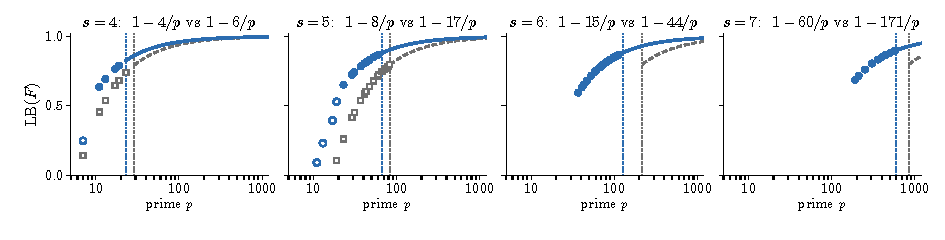
\includegraphics[width=\linewidth]{fig_freediag.pdf}
\caption{$\LB(F)$ of Theorem~\ref{thm:block} against $p$. Grey: $U^*_s$ (dashed: $1-(a^*_s+1)/p$, written proof for $p\ge5a^*_s+4$; squares: exact values, c.a.). Blue, all c.a.: the free diagonal of (d) (solid: $1-(A+1)/p$ past the threshold of Lemma~\ref{lem:signclass}; dots: exact values below it; circles: the quoted values at $p=7$, $11\le p\le19$). Dotted: the thresholds. In Lean for $s=4,5,6$ (from $p=11$, $23$, $125$), not for $s=7$.}
\label{fig:freediag}
\end{figure}

\begin{lemma}[Backward coordinates]\label{lem:signclass}
Let $F$ be a design with partial sums $M^{(j)}$, let $A\ge0$ be an integer, and let $S=\max_i\sum_c\max_j|M^{(j)}[i][c]|$. Suppose that every step $e$, with every choice of carry lengths, has a backward moving coordinate with $|\sigma_i|\le A$ or two backward moving coordinates. Then $\LB(F)\ge1-(A+1)/p$ for every prime $p>S$ with $(p-A-1)^2\le2(p-S-1)^2$.
\end{lemma}

\begin{proof}
For $p>S$ every change has $|\sigma_i|\le S<p$, so a backward coordinate contributes $c_{|\sigma_i|+1}$ (proof of Theorem~\ref{thm:block}(iii)). The term of the step is at least $c_{A+1}$ in the first case and at least $\sqrt2\,c_{S+1}\ge c_{A+1}$ in the second.
\end{proof}

The hypothesis does not depend on $p$ and is a finite check. Diagonal dominance is the case in which every moving coordinate is backward; for $U^*_s$ ($A=a^*_s$, $S\le2a^*_s$) the lemma gives the range $p\ge(3+\sqrt2)a^*_s+1$ above.

\begin{proof}[Proof of Theorem~\ref{thm:block}(d)]
Reachability is that of (c). The hypothesis of Lemma~\ref{lem:signclass} holds with $A=3$, $7$, $14$, $59$ and $S=8$, $23$, $46$, $211$ (exhaustive check, computer-assisted), which gives $\LB(F)\ge1-(A+1)/p$ for every prime $p\ge23$, $67$, $127$, $587$. Below these primes $\LB(F)$ was evaluated exactly at every prime of the stated ranges (computer-assisted; for $s=5$ it is $1/11$, $3/13$, $3\sqrt5/17$, $\sqrt{101}/19$ at $p=11,\dots,19$), and Theorem~\ref{thm:block}(iii) applies. For $s=4,5$ the bound is attained by the axis step at the place $0$ (its column of $F_0$ is $(1,\dots,1)$ off the diagonal, and $\delta_0=A$), for $s=6$ by the axis step at the place $\frac13$ with carry length $4$.
\end{proof}

How far can the diagonal go? With the off-diagonal entries of $U^*_s$ fixed, the least $A$ in Lemma~\ref{lem:signclass} gives $\lim_{p\to\infty}p(1-\LB(F))=A+1$ (a step whose only backward coordinate has $|\sigma_i|=A$ has the term $1-(A+1)/p+O(p^{-2})$). An axis step forces $0\le\delta_c\le A$, and an exhaustive search over $\delta\in[0,A]^s$ finds no diagonal with $A\le2$, $6$, $13$ for $s=4,5,6$ (computer-assisted): in this sense $4$, $8$, $15$ are optimal. For $s=7$, $60$ is the best found, against $a^*_7+1=171$.

For $s=4$ the design of Theorem~\ref{thm:block}(c) is, in the order of the places $0,1,\frac12,\frac13$ and with $v=(1,1,2,3)$,
\[
F_0=\begin{pmatrix}-5&2&1&2\\1&-3&-1&-1\\1&2&-5&-2\\1&1&1&-3\end{pmatrix},\quad
F_1=\begin{pmatrix}0&-3&-1&-1\\-2&0&2&1\\-1&-1&0&3\\0&-1&0&0\end{pmatrix},\quad
F_2=\begin{pmatrix}0&2&0&-1\\2&0&-2&0\\0&-1&0&-2\\-1&0&-1&0\end{pmatrix};
\]
the largest diagonal entry is $a^*_4=5$, and the design of (d) replaces the diagonal of $F_0$ by $-3$. Table~\ref{tab:block} collects the data. Figure~\ref{fig:block} shows the case $s=2$, $p=7$ inside and outside the family.

\begin{table}[t]
\centering
\footnotesize
\caption{The block-periodic residue sequences of Theorem~\ref{thm:block} ($\Lev=s^2\N$). Places and row constants: $(0,1)$, $(1,1)$ for $s=2$; $(0,2,1)$, $(\frac12,\frac12,-1)$ for $s=3$; $(0,1,\frac12,\dots,\frac1{s-1})$, $(1,1,2,\dots,s-1)$ for $s\ge4$. ``$U^*_s$, $\delta$'': $U^*_s$ off the diagonal, $F_0[c][c]=-\delta_c$. ``proof'': written proof; ``c.a.'': computer-assisted (exact $\LB(F)$, and for (d) Lemma~\ref{lem:signclass}); each for every prime in the range; in parentheses, further primes with $\LB(F)>0$.}
\label{tab:block}
\setlength{\tabcolsep}{4pt}
\begin{tabular}{@{}c l l l l@{}}
\toprule
$s$ & design & $\LB(F)$ & proof & c.a.\\
\midrule
2 & $F_0=\bigl(\begin{smallmatrix}-1&1\\-1&-1\end{smallmatrix}\bigr)$ & $1-2/p$ & $p\ge3$ & --\\
3 & $(M,J)$, Thm.~\ref{thm:block}(b) & $1-2/p$ & $p\ge5$ & --\\
4 & $U^*_4$ (above) & $1-6/p$ & $p\ge29$ & $7\le p\le109$\\
5 & $U^*_5$ & $1-17/p$ & $p\ge84$ & $19\le p\le109$\\
$\ge4$ & $U^*_s$ & $1-(a^*_s+1)/p$ & $p\ge5a^*_s+4$ & --\\
4 & $U^*_4$, $\delta=(3,3,3,3)$ & $1-4/p$ & -- & $p\ge11$ ($7$)\\
5 & $U^*_5$, $\delta=(7,7,7,7,7)$ & $1-8/p$ & -- & $p\ge23$ ($11$--$19$)\\
6 & $U^*_6$, $\delta=(3,12,13,14,13,13)$ & $1-15/p$ & -- & $p\ge37$ ($17$--$31$)\\
7 & $U^*_7$, $\delta=(41,44,59,57,56,6,32)$ & $1-60/p$ & -- & $p\ge191$ ($17$--$23$, $31$--$181$)\\
\bottomrule
\end{tabular}
\end{table}

\begin{figure}[t]
\centering
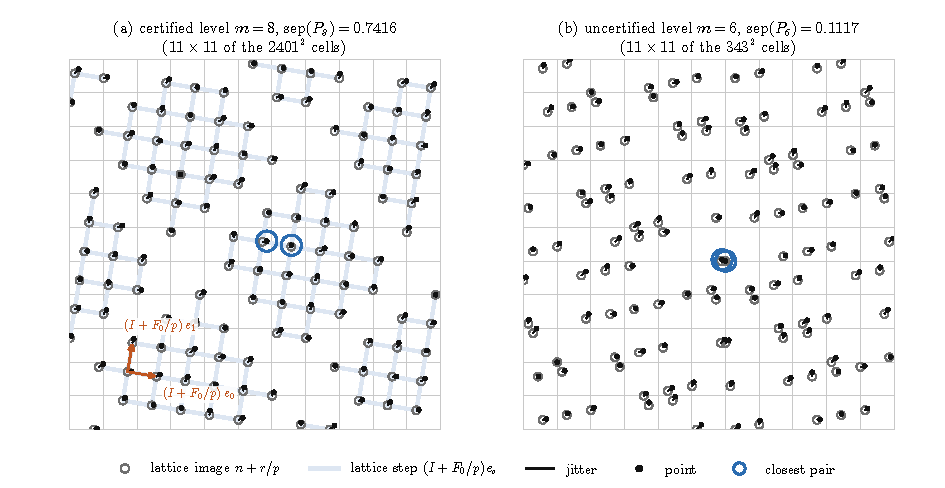
\includegraphics[width=0.9\linewidth]{fig_block.pdf}
\caption{The block-periodic residue sequence of Theorem~\ref{thm:block}(a), $s=2$, $p=7$, places $(0,1)$, $\theta=1$ (exact points). (a)~The full level $m=8$ ($2401\times2401$ cells), $11\times11$ cells around the closest pair: each point (dot) lies within one unit of the last digit of its lattice image $n+r/p$ (open circle); where no geometric digit wraps, neighbouring lattice images differ by a column of $I+F_0/p$ (light segments): patches of $\Z^2$ rotated by $\arctan(1/6)$, scaled by $\sqrt{37}/7\approx0.87$, separated by slip planes. Exact $\sep{P_8}=0.7416$ ($0.7613$ at $m=4$), certified bound $1-2/7=0.7143$. (b)~The full level $m=6$, which is not in the family $4\N$: its geometric digits are not designed, and the closest pair is only $0.1117$ cell units apart (exact).}
\label{fig:block}
\end{figure}

\begin{remark}[Exact separations and the levels in between]\label{rem:blockexact}
Exact values (illustration only) are close to the certified ones: for $s=2$, $\sep{P_4}=0.5730$, $\sep{P_8}=\sep{P_{12}}=0.3862$ and $\sep{P_{16}}=0.3610$ at $p=3$ (bound $1/3$); $0.6237$ at $m=4,8$ for $p=5$ (bound $0.6$); $0.8383$, $0.8604$, $0.8909$, $0.9016$, $0.9177$ at $m=4$ for $p=11$, $13$, $17$, $19$, $23$; for $s=3$, $\sep{P_9}=0.6211$ at $p=5$ ($\theta=1$; bound $0.6$) and $0.7378$ at $p=7$ (bound $0.7143$); at $p=3$, where the bound of (b) is $0$, $\sep{P_9}=0.4381$. Outside the family the separation is not controlled: for $s=2$, $p=5$ the levels $m=2,3,5,6,7,9,10$ have $0.368$, $0.366$, $0.276$, $0.159$, $0.354$, $0.092$, $0.159$ (evidence, not a claim).
\end{remark}

\emph{All $N$.} The family $s^2\N$ has largest gap $s^2$, so Lemma~\ref{lem:prefix} gives $\delta(P_{[N]})N^{1/s}\ge\LB(F)\,p^{-s}$ for every $N\ge2$ and the mesh ratio $h/\delta\le\sqrt s\,p^{s+1}/\LB(F)$: these sequences are quasi-uniform, the strongest of our constructions \emph{at} their certified sizes, but for all $N$ weaker than the residue sequences of Section~\ref{sec:residue}, whose bound $\LB/p$ is larger whenever $p>2^s$ (for $s=2$, $p=5$: $0.024$ against $0.089$).

\emph{The lost $1/p$.} The nets of \cite{Gru26geo} with the layer $(M,J)$ reach $1-1/q$ at every full level for $q\ge8$%
. The difference is the axis step: in the nets the deeper digits of a coordinate do not depend on its own cell%
, so an axis step has no jitter in the moving coordinate; here it has, and $1-1/p$ becomes $1-2/p$. Whether free data in the scramble can restore $1-1/p$ is open.

\subsection{Two Level Families from One Scramble}\label{sec:blocktwo}
With a block period $\ell>s$ the scramble has $\ell-s$ local multipliers left over. Giving them to a second check vector adds skeleton relations of the residue sequence at most levels in between.

\begin{theorem}[Two level families from one scramble]\label{thm:blocktwo}
Let $\ell>s$ in Definition~\ref{def:block}, with the second check vector $v'$. Then:
\begin{enumerate}
\item[(i)] the sequence is a digital $(0,s)$-sequence over $\F_p$;
\item[(ii)] for every $K\ge1$ and $\deg V<s\ell K$, $y_{i,\ell K}(V)=\sum_c\sum_{n=0}^{s-2}F_n[i][c]\,y_{c,\ell K-1-n}(V)$, and $\sep{P_{s\ell K}}\ge\LB(F)$;
\item[(iii)] for every $T\equiv1,\dots,\ell-s\pmod\ell$ and $\deg V\le s(T+1)-2$, $\sum_cv'_c\,y_{c,T}(V)=0$, and $\sep{P_{s(T+1)-1}}\ge p^{-1/s}\ljit(\Lambda_{v'})$.
\end{enumerate}
So one scramble is certified on the design levels $m\in s\ell\N$, with the constants of Theorem~\ref{thm:block}, and on the skeleton levels $m=s(T+1)-1$, $T\equiv1,\dots,\ell-s\pmod\ell$, with those of Theorem~\ref{thm:residue}: a fraction $1/\ell$ of the full levels and a fraction $(\ell-s)/\ell$ of the levels $m\equiv-1\pmod s$. For instance $s=2$, $\ell=4$: design levels $8\N$, skeleton levels $3,5,11,13,19,21,\dots$; $s=2$, $\ell=3$: $6\N$ and $3,9,15,\dots$; $s=3$, $\ell=4$: $12\N$ and $5,17,29,\dots$.
\end{theorem}

\begin{proof}
(i) As in Theorem~\ref{thm:block}(i), with $\Omega$ of order $\ell$: the design multipliers vanish to the orders $0,\dots,s-2$, the skeleton multipliers $w^{\ell-1-j}/v'_c$ to the orders $\ell-1-j\in\{s-1,\dots,\ell-2\}$, and the own multiplier to the order $\ell-1$. So $\varphi_{c,j}$ vanishes to order exactly $\ell-1-j$ for every $j$, digit $\ell n+j$ is the residue against a polar differential of exact order $\ell n+j+1$, and Lemma~\ref{lem:t0} applies.
(ii) The proof of Theorem~\ref{thm:block}(ii),(iii) is unchanged: it uses only (a), (c) and $\deg(Vu_i\Omega^{-K})\le-2$, which holds for $\deg V<s\ell K$; at $P_{s\ell K}$ the geometric digit is digit $\ell K$.
(iii) Write $T=\ell n+j$ with $1\le j\le\ell-s$. Then $v'_cy_{c,T}(V)=\Res_{a_c}(Vw^{\ell-1-j}\Omega^{-n-1}dz)=\theta^{n+1}\Res_{a_c}(Vw^{-T-1}dz)$, and by Lemma~\ref{lem:resform}(c) these add up to $0$ when $\deg V\le s(T+1)-2$. This is the skeleton relation of Lemma~\ref{lem:residue-rel} at level $T+1$ with the check vector $v'$. The proof of Theorem~\ref{thm:residue} uses only $t=0$ and this relation, so it gives the bound.
\end{proof}

The trade-off is set by $\ell$: $\ell=s$ is Theorem~\ref{thm:block}; as $\ell$ grows, almost all levels $m\equiv-1$ are certified with the constants of the residue sequence, and the full design appears on a sparser family. Exact computations agree with both bounds, e.g.\ for $s=2$, $\ell=4$, $p=5$, $v'=(2,4)$: $\sep{P_m}=0.5999$, $0.6264$, $0.4995$ at the skeleton levels $m=3,5,11$ (bound $0.4472$) and $0.6787$ at the design level $m=8$ (bound $0.6$). For all $N$ the largest gap between certified levels is still of order $s^2$ (exactly $s^2-s+1$, for every $\ell>s$), so Lemma~\ref{lem:prefix} gives no improvement over the residue sequence.

\subsection{A Skeleton Relation Implied by the Design}\label{sec:implied}
Even with $\ell=s$ the design can carry a skeleton relation at the level just after the design level, provided its diagonal is chosen for it.

\begin{proposition}[A skeleton relation implied by the design]\label{prop:implied}
In Definition~\ref{def:block} (any $\ell\ge s$), let $\bar v\in(\F_p^*)^s$ satisfy
\[
\bar v_i=\xi\,v_i/w'(a_i)\quad\text{for one }\xi\in\F_p^*,\qquad\text{and}\qquad \bar v^{\mathsf T}F_n\equiv0\pmod p\quad\text{for every }n\le s-2 .
\]
Then $\sum_i\bar v_i\,y_{i,\ell K}(V)=0$ for every $K\ge0$ and every $V$ with $\deg V\le s(\ell K+1)-2$: the skeleton relation with check vector $\bar v$ holds at the level $m=s(\ell K+1)-1$, in addition to the design at $m=s\ell K$. Consequently $\sep{P_{s(\ell K+1)-1}}\ge p^{-1/s}\ljit(\Lambda_{\bar v})$ for every $K\ge0$.
\end{proposition}

\begin{proof}
Keep the coefficient at infinity in the proof of Theorem~\ref{thm:block}(ii): by Lemma~\ref{lem:resform}(c), for every $V$,
\[
y_{i,\ell K}(V)=\sum_c\sum_{n=0}^{s-2}F_n[i][c]\,y_{c,\ell K-1-n}(V)+v_i^{-1}\,[z^{-1}]\bigl(Vu_i\Omega^{-K}\bigr)
\]
(for $K=0$ the sum is empty). Multiply by $\bar v_i$ and sum over $i$. The double sum vanishes because $\bar v^{\mathsf T}F_n\equiv0$. By partial fractions $\sum_iu_i/w'(a_i)=1/w$, so the rest is $\xi[z^{-1}](V\Omega^{-K}/w)=\xi\theta^K[z^{-1}](V/w^{\ell K+1})$, which is $0$ for $\deg V\le s(\ell K+1)-2$. The bound follows as in Theorem~\ref{thm:residue}.
\end{proof}

The condition $\bar v^{\mathsf T}F_n\equiv0$ can always be met by the free diagonal, choosing $F_n[c][c]$ with $\bar v_cF_n[c][c]=-\sum_{i\ne c}\bar v_iF_n[i][c]$. But it has a price. It says that every column of every $F_n$, read as an integer vector of centred residues, lies in $\Lambda_{\bar v}$. Hence
\[
\ljit(\Lambda_{\bar v})\ \le\ \min\bigl\{\|(|F_n[\cdot][c]|-\mathbf 1)_+\|_2:\ n\le s-2,\ F_n[\cdot][c]\ne0\bigr\},
\]
so a good implied skeleton relation (with $\ljit(\Lambda_{\bar v})$ of order $p^{1/s}$) forces an entry of order $p^{1/s}$ in every nonzero column of the design, far from the entries $\pm1$ of the nets. (For example a column $(-2,-1)$ forces $\ljit\le1$.) In dimension two the price can be paid exactly at the primes one more than a square.

\begin{corollary}[Primes of the form $u^2+1$]\label{cor:gauss}
Let $p=u^2+1$ be a prime ($u$ even: $p=5,17,37,101,197,257,401,\dots$), $s=\ell=2$, places $(0,1)$, $v=(-u,-1)$ and $F_0=\bigl(\begin{smallmatrix}-1&u\\-u&-1\end{smallmatrix}\bigr)$. Then for every $K\ge1$
\[
\begin{aligned}
\sep{P_{4K}}&\ \ge\ \frac{\sqrt{(u-2)^2+(u^2-u-1)^2}}p\ \ge\ 1-\frac{\sqrt{p-1}+2}p,\\
\sep{P_{4K+1}}&\ \ge\ \frac{u-1}{\sqrt p}=\frac{\sqrt{p-1}-1}{\sqrt p}.
\end{aligned}
\]
The fine cells occupied by $P_{4K+1}$ form the square lattice $\Z(1,u)+\Z(u,-1)$.
\end{corollary}

\begin{proof}
For $s=2$ reachability only asks for nonzero crosses. With $w=z^2-z$, $w'(0)=-1$, $w'(1)=1$, the vector $\bar v=(u,-1)$ satisfies $\bar v_i=v_i/w'(a_i)$, and $\bar v^{\mathsf T}F_0=(-u+u,\,u^2+1)\equiv0$. \emph{Design levels.} The carry length does not matter, and the four steps give $\sigma=(-1,-u)$, $(u,-1)$, $(u-1,-u-1)$ and $(-u-1,1-u)$. The axis steps have the terms $\bigl((p-2)^2+(u-1)^2\bigr)^{1/2}/p\ge(p-2)/p$. On the diagonal steps the two coordinates contribute $(u-2)/p$ and $(p-u-2)/p=(u^2-u-1)/p$, and $(p-2)^2-(p-u-2)^2-(u-2)^2=2pu-2u^2-4>0$, so the diagonal term is the minimum; it is at least $(p-u-2)/p$. \emph{Skeleton levels.} By Proposition~\ref{prop:implied} the skeleton relation with $\bar v$ holds at $m=4K+1$. The lattice $\Lambda_{\bar v}=\{b:ub_0\equiv b_1\}$ contains $(1,u)$ and $(u,-1)$, whose determinant is $-p$, so they span it, and $|m(1,u)+n(u,-1)|^2=(m^2+n^2)p$. The four vectors $\pm(1,u)$, $\pm(u,-1)$ have $\|(|b|-\mathbf 1)_+\|_2=u-1$, and every other nonzero vector has length at least $\sqrt{2p}$, hence $\|(|b|-\mathbf 1)_+\|_2\ge\sqrt{2p}-\sqrt2\ge u-1$. So $\ljit(\Lambda_{\bar v})=u-1$, and Theorem~\ref{thm:residue} applies.
\end{proof}

At the skeleton levels $\bar v=(u,-1)$ is the Korobov vector of Corollary~\ref{cor:korobov} ($\rho=u$), so the bound is the Korobov bound $(\rho-1)p^{-1/2}$ of the residue sequence; it is about $1-p^{-1/2}$, against the general lower form $1-2p^{-1/2}$, because the fine-cell lattice is an exact square. It is the best over all check vectors at $p=5$, $17$, $37$, $197$, not at $p=101$, $257$, $401$, where other check vectors have a larger $\ljit^2$ ($85$, $241$, $369$ against $81$, $225$, $361$; exact computation). At the design levels the constant is $1-O(p^{-1/2})$, below the $1-2/p$ of Theorem~\ref{thm:block}(a): the price of the implied relation. Exact computations agree: $\LB(F)=0.6576$, $0.7912$, $0.8847$ at $p=17$, $37$, $101$, against $\sep{P_4}=0.6597$, $0.8072$, $0.8885$; at the skeleton level $m=5$, $\sep{P_5}=0.6406$, $0.7988$, $0.9094$ at $p=5$, $17$, $37$, against $0.4472$, $0.7276$, $0.8220$.

\begin{remark}[Meeting the density bound]\label{rem:gaussfrontier}
For $s=2$ and $\ell\ge3$, adding the skeleton multipliers of Theorem~\ref{thm:blocktwo} to the design of Corollary~\ref{cor:gauss} certifies the design at $m\in2\ell\N$ and the skeleton relation at the levels $m=2N+1$ with $N\not\equiv-1\pmod\ell$, i.e.\ at a fraction $(\ell-1)/\ell$ of the levels $m\equiv1\pmod2$ (Theorem~\ref{thm:blocktwo}(iii) and Proposition~\ref{prop:implied}). The two densities add up to $1$, the largest value that exact relations of bounded depth allow (Corollary~\ref{cor:density}). The bound for all $N$ does not improve on that of the residue sequence: the largest gap between certified levels is $3$, against $2$ for the residue sequence.
\end{remark}

%
%
%
%
%
%
%
%
\section{How Many Exact Relations a Sequence Can Carry}\label{sec:count}
The nets of \cite{Gru26geo} reach separations $1-O(1/q)$ at the full levels by designing the whole geometric layer: at one prefix, every geometric digit is a prescribed linear function of the last few cell digits%
. These are $s$ exact linear identities among the digits of the points, and the nets choose them anew for every size. Sections~\ref{sec:residue} and~\ref{sec:block} install such identities in one fixed scramble, by the residue theorem. The staggered residue sequence carries one at every full level, the residue sequence one at every prefix $P_{sK-1}$ (its skeleton relation), the block-periodic residue sequences carry $s$ of them at every $s$-th full level, and the sequences of Theorem~\ref{thm:blocktwo} and Corollary~\ref{cor:gauss} share the levels between two families. In every case this is about one identity per level. Why not $s$ at every full level? That would put the designed lattice of the nets into every full level of one sequence, with constants $1-O(1/p)$ at every full level and the best bound for all $N$ (Lemma~\ref{lem:prefix}).

This section shows that, for exact relations of bounded depth, about one per level is the limit. The reason is a shortage of digits. Without a depth bound every full level carries $s$ exact relations, namely the offset map itself: each geometric digit is a linear function of all the cell digits. A relation of depth at most $J$ at level $T$ uses, in a given coordinate, only the digits $T-J,\dots,T$, and the residue theorem shows that relations at different levels cannot share these digits: each relation needs a digit position of its own. A range of $R+1$ consecutive levels offers $J+R+1$ digit positions in one coordinate, so it carries at most $J+R+1$ independent relations, about one per level (Theorem~\ref{thm:count} and Figure~\ref{fig:count}).

\emph{Scope.} All results of this section are negative, and each holds in exactly this scope. The sequences are the lower-triangular scrambles $C_c=L_c\Pas_{a_c}$ of a frame of $s$ distinct places in $\F_q$, the class of Lemma~\ref{lem:t0}; it contains every sequence of Sections~\ref{sec:law}--\ref{sec:block} and every generalized Faure sequence. The certificates are exact linear identities among the digits, of bounded depth (Definition~\ref{def:exactrel}), whose coefficients may depend on the level. Every statement names its range of levels. Linearity is no restriction for a designed digit: if a geometric digit is a function of the last $J$ cell digits at all, it is a linear one, because the offset map is linear and the cell digits are free. Exactness is a restriction. The windows of Section~\ref{sec:antipode} keep responses in sets of allowed values instead of fixing them; they are not exact relations, and they do certify every full level. Digital sequences that are not frame scrambles (for instance Niederreiter sequences with bases of degree at least two, or sequences with $t>0$) are not covered either.

\subsection{Exact Digit Relations}\label{sec:countdef}
Fix a frame $(a_0,\dots,a_{s-1};\infty)$ over $\F_q$ with distinct places, $s\ge2$, and a scramble $(L_c)$; put $w=\prod_c(z-a_c)$. By Lemma~\ref{lem:resform}(a) digit $n$ of coordinate $c$ is $y_{c,n}(V)=\Res_{a_c}(V\eta_{c,n})$ with a polar differential $\eta_{c,n}$ at $a_c$ of exact pole order $n+1$; so $\eta_{c,0},\dots,\eta_{c,T}$ are a basis of the polar differentials at $a_c$ of pole order at most $T+1$. For a rational function $F$ we write $\operatorname{pp}_a(F\,dz)$ for the principal part of $F\,dz$ at $a$: the terms $(z-a)^{-k}dz$, $k\ge1$, of its expansion.

\begin{definition}[Exact digit relation]\label{def:exactrel}
Let $T\ge0$ and $m\ge sT$. An \emph{exact digit relation of top index $T$ on $P_m$} is a family of coefficients $f_{c,n}\in\F_q$ ($0\le c<s$, $0\le n\le T$), not all zero, with
\[
\sum_c\sum_{n\le T}f_{c,n}\,y_{c,n}(V)=0\qquad\text{for every }V\text{ with }\deg V<m .
\]
It has \emph{depth at most $J$ at coordinate $c$} if $f_{c,n}=0$ for $n<T-J$, and \emph{depth at most $J$} if this holds at every coordinate.
\end{definition}

A relation on $P_m$ is also a relation on every smaller prefix $P_{m'}$, $sT\le m'\le m$, so the relations of top index $T$ on $P_{sT}$ contain all others; they form a vector space. The examples of this paper:
\begin{enumerate}
\item[(1)] A \emph{designed geometric digit} at the full level $P_{sT}$: $y_{i,T}=\sum_c\sum_{n=T-J}^{T-1}f_{c,n}y_{c,n}$, a relation of top index $T$ and depth at most $J$. A design in the sense of \cite{Gru26geo} is one such relation for each of the $s$ coordinates; Theorem~\ref{thm:block}(ii) gives them at $T=sK$ with depth $s-1$.
\item[(2)] The relation of the staggered residue sequence, $y_{\cstar,T}=\sum_{c\ne\cstar}k_cy_{c,T-1}$ on $P_{sT}$ (Lemma~\ref{lem:residuestar-rel}): top index $T$, depth $1$.
\item[(3)] The skeleton relation $\sum_cv_cy_{c,T}=0$ on $P_{s(T+1)-1}$ (Lemma~\ref{lem:residue-rel} at level $T+1$): top index $T$, depth $0$.
\item[(4)] The offset map: at every level $T$, each geometric digit $y_{i,T}$ is a linear function of all cell digits of $P_{sT}$. These are $s$ relations of top index $T$ on $P_{sT}$, of depth $T$.
\end{enumerate}
Example (4) shows that relations as such are not scarce; the depth bound is what makes them scarce. The next lemma, the one tool of this section, translates a relation into a single polynomial.

\begin{lemma}[The polynomial of a relation]\label{lem:reltype}
Let $(f_{c,n})$ be an exact digit relation of top index $T$ on $P_m$, $m\ge sT$. There is a unique polynomial $A\ne0$ of degree at most $s(T+1)-m-1\le s-1$ with
\[
\sum_{n\le T}f_{c,n}\,\eta_{c,n}=\operatorname{pp}_{a_c}\bigl(A\,w^{-T-1}dz\bigr)\qquad\text{for every }c .
\]
The map from relations to polynomials is linear and injective, and $f_{c,T}\ne0$ exactly for the coordinates $c$ with $A(a_c)\ne0$. Conversely, every nonzero polynomial of degree at most $s(T+1)-m-1$ is the polynomial of exactly one relation of top index $T$ on $P_m$. Hence these relations form a space of dimension $s(T+1)-m$ (if $m\le s(T+1)$): $s$ on the full level $P_{sT}$, and $1$ on $P_{s(T+1)-1}$.
\end{lemma}

\begin{proof}
Put $\eta_c=\sum_nf_{c,n}\eta_{c,n}$, a polar differential at $a_c$ of pole order at most $T+1$, and $\eta=\sum_c\eta_c=\Xi\,dz$. The rational function $\Xi$ has poles only at the places, of order at most $T+1$, and vanishes at $\infty$; so $\Xi =A/w^{T+1}$ with a polynomial $A$ of degree less than $s(T+1)$. Since $\eta_{c'}$ is regular at $a_c$ for $c'\ne c$, $\eta_c$ is the principal part of $\Xi\,dz$ at $a_c$. For a polynomial $V$, the differential $V\eta_c$ has the same residue at $a_c$ as $V\Xi\,dz$, so by Lemma~\ref{lem:resform}(c)
\[
\sum_c\sum_nf_{c,n}\,y_{c,n}(V)=\sum_c\Res_{a_c}(V\Xi\,dz)=[z^{-1}]\,(V\Xi).
\]
This vanishes for all $V$ of degree less than $m$ if and only if the coefficients of $z^{-1},\dots,z^{-m}$ in the expansion of $\Xi$ at $\infty$ vanish, that is, if and only if $A=0$ or $s(T+1)-\deg A\ge m+1$. If $A=0$, then every $\eta_c=\operatorname{pp}_{a_c}(\Xi\,dz)=0$, and all $f_{c,n}=0$ because the $\eta_{c,n}$ are linearly independent; so $A\ne0$ and $\deg A\le s(T+1)-m-1$. Uniqueness and linearity are clear, since $A=\Xi w^{T+1}$, and injectivity is the argument just given. The pole order of $\operatorname{pp}_{a_c}(Aw^{-T-1}dz)$ is $T+1$ exactly when $A(a_c)\ne0$, which is the statement about $f_{c,T}$. Conversely, given $A$, write $\operatorname{pp}_{a_c}(Aw^{-T-1}dz)$ in the basis $\eta_{c,0},\dots,\eta_{c,T}$; the computation above, read backwards, shows that the coefficients form a relation on $P_m$.
\end{proof}

So on a full level there are exactly the $s$ relations of the offset map, and on $P_{s(T+1)-1}$ exactly one: in the language of Section~\ref{sec:residueseq}, the skeleton digit of a skeleton coordinate is always a linear function of the other digits, and the residue sequence is the case in which this function has depth zero (Lemma~\ref{lem:rigid} below makes this precise). The numerator $A$ also tells which digits a relation involves. A designed geometric digit of coordinate $i$ has $f_{c,T}=0$ for $c\ne i$, so $A$ vanishes at the $s-1$ places $a_c$, $c\ne i$: $A$ is a multiple of $w_i=w/(z-a_i)$. The staggered relation (2) has $A$ a multiple of $w_{\cstar}$, and the skeleton relation (3) has a constant $A$.

\subsection{Counting Exact Digit Relations}\label{sec:countthm}
We call a range of levels $[K_0,K_0+R]$ \emph{admissible for depth $J$} if
\[
K_0\ge J\qquad\text{and}\qquad K_0>(s-1)R+s-2 .
\]
Every subrange $[K_0,K_0+R']$, $R'\le R$, of an admissible range is admissible, and for fixed $J$ every level $K_0\ge\max(J,s-1)$ starts an admissible range of length about $K_0/(s-1)$.

\begin{theorem}[Counting exact digit relations]\label{thm:count}
Let $[K_0,K_0+R]$ be admissible for depth $J$, and fix a coordinate $c$. For every level $T\in[K_0,K_0+R]$ let $r_T$ be the dimension of a space of exact digit relations of top index $T$ on $P_{sT}$ whose depth at coordinate $c$ is at most $J$ (the depth at the other coordinates is arbitrary, and the coefficients may depend on $T$). Then
\[
\sum_{T=K_0}^{K_0+R}r_T\ \le\ J+R+1 .
\]
More precisely, $\sum_Tr_T$ is at most the number of digit positions $n$ of coordinate $c$ at which at least one of these relations has a nonzero coefficient.
\end{theorem}

\begin{proof}
Choose a basis of each of the spaces and let $\mathcal N_c$ be the set of digit positions $n$ of coordinate $c$ used by some basis relation; $\mathcal N_c\subseteq[K_0-J,K_0+R]$, so $|\mathcal N_c|\le J+R+1$. The \emph{place-$c$ part} $\sum_nf_{c,n}\eta_{c,n}$ of each basis relation lies in the span of $\{\eta_{c,n}:n\in\mathcal N_c\}$, which has dimension $|\mathcal N_c|$. It suffices to show that the place-$c$ parts of all $\sum_Tr_T$ basis relations are linearly independent.

Suppose a linear combination of them vanishes. Group it by levels: the part at level $T$ is a relation of top index $T$ on $P_{sT}$ or zero, with a polynomial $A_T$ of degree at most $s-1$ (Lemma~\ref{lem:reltype}; $A_T=0$ if the part is zero), and the vanishing says that $\sum_T\operatorname{pp}_{a_c}(A_Tw^{-T-1}dz)=0$. Put $T^*=K_0+R$. Then
\[
\sum_TA_T\,w^{-T-1}=w^{-T^*-1}B,\qquad B=\sum_TA_T\,w^{T^*-T},\qquad \deg B\le sR+s-1,
\]
and $w^{-T^*-1}B$ has no principal part at $a_c$. As $w$ is $z-a_c$ times a unit at $a_c$, this means that $(z-a_c)^{T^*+1}$ divides $B$. But $T^*+1=K_0+R+1>sR+s-1\ge\deg B$ by admissibility, so $B=0$. Since $\deg A_T<s=\deg w$, the expansion $B=\sum_TA_Tw^{T^*-T}$ is the $w$-adic expansion of $B$, which is unique; hence every $A_T=0$, and by Lemma~\ref{lem:reltype} every level part is the zero relation. The basis relations at each level are independent, so all coefficients of the combination vanish.
\end{proof}

The proof uses one place only, and nothing about the scramble beyond its residue form; it holds over every $\F_q$. The admissibility condition cannot be dropped. For $s=2$ and $J=1$, take the range $[1,2]$, which has $K_0=1\ge J$ but violates $K_0>(s-1)R+s-2=1$. At level $1$ every frame scramble has two relations of depth at most $1$, the offset map of $P_2$, since a single cell digit per coordinate is all there is. At level $2$ the block-periodic residue sequence of Theorem~\ref{thm:block}(a) designs both geometric digits of $P_4$ with depth $1$. That is $4>J+R+1=3$ relations. So for $s=2$ and $J=1$ the threshold $K_0\ge2$ is sharp.

\begin{figure}[t]
\centering
\paperfig{fig_count}
\caption{Why exact relations are scarce (Theorem~\ref{thm:count}), for $s=2$ and the range of levels $T=6,\dots,11$, which is admissible for depth $J=1$. Each column is a level $T$; each row is a digit position $n$ of coordinate~$0$. A relation of top index $T$ is drawn as a bar in column $T$ covering the digit positions at which it has nonzero coefficients in coordinate~$0$ (depth $J=1$: positions $T-1$ and $T$). The parts in coordinate~$0$ of all relations of the range are linearly independent (proof of Theorem~\ref{thm:count}), so there are at most as many bars as rows touched (black squares). (a)~The residue sequence: one skeleton relation per level, at position $T$ (Lemma~\ref{lem:residue-rel}). (b)~The block-periodic residue sequence of Theorem~\ref{thm:block}(a): both geometric digits designed at the even levels (Theorem~\ref{thm:block}(ii)); the relation of coordinate~$0$ uses the positions $T-1$ and $T$, that of coordinate~$1$ only $T-1$; no relation at the odd levels. (c)~Both geometric digits designed with depth $1$ at every level would need twelve bars on seven rows; Corollary~\ref{cor:layer}(b) excludes it.}
\label{fig:count}
\end{figure}

\begin{corollary}[Designed geometric digits]\label{cor:layer}
Let $J\ge0$, and consider a scramble of a frame of $s\ge2$ distinct places over $\F_q$.
\begin{enumerate}
\item[(a)] Let $E$ be the set of levels $T$ at which all $s$ geometric digits of $P_{sT}$ are designed by exact relations of depth at most $J$. Then $|E\cap[K_0,K_0+R]|\le(J+R+1)/s$ for every admissible range, and $\limsup_{X\to\infty}|E\cap[1,X]|/X\le1/s$. Theorem~\ref{thm:block} attains the density $1/s$.
\item[(b)] Two geometric digits, of coordinates $i\ne i'$, are not both designed with depth at most $J$ at all the levels $K_0,\dots,K_0+J$, if $K_0>(s-1)J+s-2$.
\item[(c)] A relation of the form $y_{\cstar,T}=\sum_{c\ne\cstar}k_cy_{c,T-1}$ on $P_{sT}$ (as for the staggered residue sequence) and a skeleton relation $\sum_cv_cy_{c,T}=0$ on $P_{s(T+1)-1}$ (as for the residue sequence), with any coefficients, do not both hold at two consecutive levels $T=K_0,K_0+1$ with $K_0\ge2s-2$.
\end{enumerate}
\end{corollary}

\begin{proof}
(a) The $s$ design relations at a level $T\in E$ are independent, since the relation of coordinate $i$ has the coefficient $1$ at $y_{i,T}$ and $0$ at $y_{i',T}$, $i'\ne i$. Theorem~\ref{thm:count} gives $s|E\cap[K_0,K_0+R]|\le J+R+1$. For the density, cover the levels from $T_1=\max(J,4s)$ to $X$ by consecutive admissible ranges $[T_k,T_k+R_k]$ with $R_k=\lfloor(T_k-s+1)/(s-1)\rfloor$ and $T_{k+1}=T_k+R_k+1$, the last one cut at $X$. Then $(s-1)R_k\le T_k-s+1$ gives admissibility, and $T_k\ge4s$ gives $R_k+1\ge T_k/(2s-2)$, so the ranges grow geometrically and there are $O(s\log X)$ of them. Summing the bound over the ranges, $|E\cap[1,X]|\le T_1+(X+J\cdot O(s\log X))/s$, and the density statement follows. Theorem~\ref{thm:block} designs all geometric digits at the levels $T\in s\N$.
(b) The two design relations at each level are independent (as in (a)), so the range $[K_0,K_0+J]$, which is admissible, would carry $2(J+1)>2J+1$ relations.
(c) Both relations have top index $T$ and depth at most $1$, and they are independent: the first has a polynomial $A$ that is a nonzero multiple of $w_{\cstar}$, of degree $s-1\ge1$, and the second a constant one (Lemma~\ref{lem:reltype} and the remark after it). The range $[K_0,K_0+1]$ is admissible for $J=1$ when $K_0>2s-3$, and would carry $4>3$ relations.
\end{proof}

The case $s=2$, $J=1$ of the one-place form is the obstruction stated in Section~\ref{sec:law}: no scramble of the frame $(0,1;\infty)$ in dimension two has a sheared lattice without jumps at two consecutive levels $K,K+1\ge2$. We state it as a corollary; Appendix~\ref{app:responses} gives a direct proof, which needs even less: only that coordinate~$0$ is lower triangular and that $P_{2K}$ and $P_{2K+2}$ are nets.

\begin{corollary}[No lattice offset map]\label{cor:N1}
Let $s=2$, $a_0=0$, $a_1=1$, $K\ge2$, and let $(L_0,L_1)$ be any scramble over any $\F_q$. The following three conditions do not hold together: the cross part of the offset map of coordinate~$0$ depends only on the finest cell digit of coordinate~$1$ at level $K$; it does so at level $K+1$; and the own part of the offset map of coordinate~$1$ depends only on the finest cell digit of coordinate~$1$ at level $K$. In particular no scramble of this frame has an offset map that depends only on the finest cell digits (a sheared lattice without jumps) at two consecutive levels $K,K+1\ge2$.
\end{corollary}

\begin{proof}
The three conditions are relations of top indices $K$, $K+1$ and $K$, on $P_{2K}$, $P_{2K+2}$ and $P_{2K}$: $y_{0,K}=X\,y_{1,K-1}+(\text{cell digits of coordinate }0)$, $y_{0,K+1}=X'\,y_{1,K}+(\text{cell digits of coordinate }0)$, and $y_{1,K}=O\,y_{1,K-1}+(\text{cell digits of coordinate }0)$. The two relations at level $K$ are independent (one has the coefficient $1$ at $y_{0,K}$ and $0$ at $y_{1,K}$, the other the reverse). In coordinate $1$ the three relations use only the digit positions $K-1$ and $K$, and the range $[K,K+1]$ is admissible for depth $1$ because $K\ge2$. The refined form of Theorem~\ref{thm:count} at coordinate $1$ gives $3\le2$, a contradiction. A finest-digit offset map at the levels $K$ and $K+1$ satisfies all three conditions.
\end{proof}

\subsection{Self-Similar and Block-Periodic Scrambles}\label{sec:countselfsim}
For a self-similar scramble the offset map is the same at every level (Proposition~\ref{prop:law}), so a relation is most useful when its coefficients do not depend on the level. Theorem~\ref{thm:count} then allows at most one such relation, and the residue form says which one.

\begin{proposition}[A self-similar scramble carries one exact relation]\label{prop:onerel}
Let the scramble be self-similar with scale $\theta$ and local multipliers $\varphi_c$ (Lemma~\ref{lem:resform}(b)), and let $J\ge0$. Call a family $\vartheta_{c,i}\in\F_q$ ($0\le c<s$, $0\le i\le J$), not all zero, a \emph{level-independent relation} if there is $T_0\ge J$ with
\[
\sum_c\sum_{i=0}^{J}\vartheta_{c,i}\,y_{c,T-i}(V)=0\qquad\text{for every }T\ge T_0\text{ and every }V\text{ with }\deg V<sT,
\]
a relation among the geometric digit $y_{c,T}$ and the last $J$ cell digits at every full level from $T_0$ on. Put $\vartheta_c(x)=\sum_i\vartheta_{c,i}x^i$.
\begin{enumerate}
\item[(i)] For every level-independent relation there is a polynomial $A\ne0$ of degree at most $s-1$ with $\varphi_c\cdot\vartheta_c(w/\theta)=A$ as power series at every place $a_c$. The level-independent relations form a space of dimension at most one.
\item[(ii)] If the relation holds on the larger prefixes $P_{sT+i}$ for every $T\ge T_0$, with $1\le i\le s-1$, then $\deg A\le s-1-i$. On the prefixes $P_{s(T+1)-1}$ ($i=s-1$), $A$ is a constant.
\item[(iii)] Let $q=p$ be prime. The scramble satisfies $y_{\cstar,T}=\sum_{c\ne\cstar}k_cy_{c,T-1}$ on $P_{sT}$ for every $T\ge T_0$ if and only if every $k_c\ne0$ and it is a staggered residue sequence $\Rstar_v$ with these weights (Definition~\ref{def:residuestar}). It satisfies a skeleton relation $\sum_cv_cy_{c,T}=0$ on $P_{s(T+1)-1}$ for every $T\ge T_0$ if and only if it is a residue sequence $\Rv_{v'}$ with scale $\theta$ and a check vector $v'$ proportional to $v$ (Definition~\ref{def:residue}). No self-similar scramble has both relations.
\end{enumerate}
\end{proposition}

\begin{proof}
(i) At level $T$, $y_{c,T-i}(V)=\Res_{a_c}(V\varphi_c(\theta/w)^{T-i+1}dz)$ and $(\theta/w)^{T-i+1}=(w/\theta)^i(\theta/w)^{T+1}$, so the place-$c$ part of the relation is $\operatorname{pp}_{a_c}(\theta^{T+1}\varphi_c\vartheta_c(w/\theta)\,w^{-T-1}dz)$. By Lemma~\ref{lem:reltype} it equals $\operatorname{pp}_{a_c}(A_Tw^{-T-1}dz)$ with a nonzero polynomial $A_T$ of degree at most $s-1$. Two functions $H_1w^{-T-1}$, $H_2w^{-T-1}$ with $H_1,H_2$ regular at $a_c$ have the same principal part there if and only if $H_1\equiv H_2\bmod(z-a_c)^{T+1}$. So $\tilde A_T:=\theta^{-T-1}A_T$ satisfies $\tilde A_T\equiv\varphi_c\vartheta_c(w/\theta)\bmod(z-a_c)^{T+1}$ at every place. Then $\tilde A_T\equiv\tilde A_{T+1}$ modulo every $(z-a_c)^{T+1}$, hence modulo $w^{T+1}$; both have degree less than $s(T+1)$, so $\tilde A_T=\tilde A_{T+1}$. Call this polynomial $A$. It is congruent to $\varphi_c\vartheta_c(w/\theta)$ modulo every power of $z-a_c$, hence equal to it as a power series, and $A\ne0$.

Let $\vartheta'$ be a second level-independent relation, with polynomial $A'$. If $A'=\lambda A$, then $\varphi_c(\vartheta'_c-\lambda\vartheta_c)(w/\theta)=0$ at every place; as $\varphi_c$ is a unit and $w/\theta$ is $z-a_c$ times a unit, $\vartheta'_c=\lambda\vartheta_c$, and the two relations are proportional. Otherwise $A/A'$ is a non-constant rational function whose numerator and denominator have degree at most $s-1$. No $\vartheta'_c$ is zero, since then $A'$ would vanish as a power series at $a_c$. In the Laurent series at $a_c$, $A/A'=\varrho_c(w)$ with $\varrho_c(x)=\vartheta_c(x/\theta)/\vartheta'_c(x/\theta)\in\F_q(x)$. This is an identity of rational functions in $z$, and $x\mapsto w$ is an injective map of fields $\F_q(x)\to\F_q(z)$, so all $\varrho_c$ are one non-constant $\varrho=P_1/P_2$ in lowest terms. Then $P_1(w)$ and $P_2(w)$ are coprime (a common root $\beta$ would make $w(\beta)$ a common root of $P_1$ and $P_2$), so $A/A'=P_1(w)/P_2(w)$ has numerator or denominator of degree $s\max(\deg P_1,\deg P_2)\ge s$. That contradicts the degree bound $s-1$.

(ii) On $P_{sT+i}$, Lemma~\ref{lem:reltype} gives $\deg A_T\le s(T+1)-(sT+i)-1=s-1-i$.

(iii) If $y_{\cstar,T}=\sum_ck_cy_{c,T-1}$, then $\vartheta_{\cstar}=1$ and $\vartheta_c(x)=-k_cx$ for $c\ne\cstar$. By (i), $A=-k_c\varphi_cw/\theta$ at $a_c$, so $k_c\ne0$ (else $A$ would vanish at $a_c$ as a power series) and $A(a_c)=0$ for every $c\ne\cstar$. As $\deg A\le s-1$, $A=\lambda w_{\cstar}$ with $\lambda\ne0$. Hence $\varphi_c=-(\lambda\theta/k_c)/(z-a_{\cstar})$ for $c\ne\cstar$ and $\varphi_{\cstar}=\lambda w_{\cstar}$: these are the local multipliers of $\Rstar_v$ with $\mu_\star=\lambda\theta$ and $\mu_c=-\mu_\star/k_c$ (Section~\ref{sec:brickwall}). If $\sum_cv_cy_{c,T}=0$ on $P_{s(T+1)-1}$, then $\vartheta_c=v_c$ and, by (ii), $A=\alpha$ is a nonzero constant; so every $v_c\ne0$ and $\varphi_c=\alpha/v_c$, the local multipliers of $\Rv_{v/\alpha}$. Conversely both sequences have their relations (Lemmas~\ref{lem:residuestar-rel} and~\ref{lem:residue-rel}). Finally, the skeleton relation on $P_{s(T+1)-1}$ holds in particular on $P_{sT}$, and its polynomial is constant, while the staggered relation has the non-constant polynomial $\lambda w_{\cstar}$; two independent level-independent relations contradict (i).
\end{proof}

\emph{Scope.} The proposition counts relations whose most significant digit is the geometric digit (or, in (ii), the digit $y_{c,T}$ read on $P_{sT+i}$). Identities among deeper digits are not extra relations: the residue sequence satisfies $\sum_cv_cy_{c,T+i}=0$ on $P_{sT}$ for every $i\ge0$ (Lemma~\ref{lem:residue-rel}), infinitely many independent identities, but for $i\ge1$ each is the skeleton relation of a later level restricted to a smaller prefix; in the sense of Definition~\ref{def:exactrel} it has top index $T+i$ and lives on a prefix smaller than $P_{s(T+i)}$. Part~(iii) explains the two constructions of Section~\ref{sec:residue}: each is the only self-similar scramble with its relation, and the remark on full levels after Theorem~\ref{thm:residue} is the last statement of (iii). Part~(ii) also bounds the nets that a self-similar sequence can imitate. The prefix $P_{s(T+1)-j}$ has $j$ skeleton coordinates, and the nets of \cite{Gru26geo} with $j$ skeleton coordinates prescribe $j$ skeleton digits%
; a self-similar scramble supplies at most one relation of bounded depth with coefficients independent of the level, so for $j\ge2$ it cannot supply them in this way.

The block-periodic scrambles of Section~\ref{sec:block} escape the count of Proposition~\ref{prop:onerel} by reading their digits in blocks. In general, a \emph{block-periodic scramble of period $\ell$} has digits $y_{c,\ell n+j}(V)=\Res_{a_c}(V\varphi_{c,j}\Omega^{-n-1}dz)$, $0\le j<\ell$, with $\Omega=w^\ell/\theta$ and power series $\varphi_{c,j}$ at $a_c$ that vanish to order exactly $\ell-1-j$; Definition~\ref{def:block} is an instance, and $\ell=1$ is a self-similar scramble. The digit $\ell n+j$ is then the residue against a polar differential of exact order $\ell n+j+1$, so this is a scramble of the frame. Its structure repeats with period $\ell$ in the level, and a relation is level-independent \emph{of class $j$} if its coefficients $\vartheta_{c,i}$ of $y_{c,T-i}$ ($i\le J$) are the same for all $T\equiv j\pmod\ell$, $T\ge T_0$, on $P_{sT}$.

\begin{proposition}[A block-periodic scramble carries $\ell$ exact relations]\label{prop:blockrel}
For a block-periodic scramble of period $\ell$ and every $J\ge0$, the level-independent relations of all classes $j=0,\dots,\ell-1$ together span a space of dimension at most $\ell$: if $d_j$ is the dimension of the space of level-independent relations of class $j$, then $d_0+\dots+d_{\ell-1}\le\ell$.
\end{proposition}

\begin{proof}
Fix a class $j$ and a relation of that class, and let $T=\ell n+j\ge T_0$. Each digit $y_{c,T-i}$ is read by $\varphi_{c,j'}\Omega^{-n'-1}dz$ with $T-i=\ell n'+j'$, and $\Omega^{-n'-1}=\Omega^{n-n'}\Omega^{-n-1}$, where $j'$ and $n-n'$ depend only on $i$ and $j$. So the place-$c$ part of the relation is $\operatorname{pp}_{a_c}(h_c\Omega^{-n-1}dz)$ with
\[
h_c=\sum_{j'<\ell}\varphi_{c,j'}\,P_{c,j'}(\Omega),
\]
where the polynomials $P_{c,j'}$ collect the coefficients $\vartheta_{c,i}$ and do not depend on $n$. The orders of vanishing of the terms $\varphi_{c,j'}P_{c,j'}(\Omega)$ at $a_c$ are $\equiv\ell-1-j'\pmod\ell$, pairwise different, so $h_c$ determines the $P_{c,j'}$, and $h_c=0$ only for the zero relation. By Lemma~\ref{lem:reltype} the place-$c$ part is also $\operatorname{pp}_{a_c}(A_Tw^{-T-1}dz)$ with $\deg A_T\le s-1$. Since $\Omega^{-n-1}=\theta^{n+1}w^{-T-1}w^{-(\ell-1-j)}$, comparing the two forms as in the proof of Proposition~\ref{prop:onerel} gives $h_c\equiv\hat A_n\bmod(z-a_c)^{\ell(n+1)}$ at every place, with the polynomial $\hat A_n=\theta^{-n-1}A_Tw^{\ell-1-j}$ of degree less than $s(\ell-j)\le s\ell$. As there, $\hat A_n$ does not depend on $n$, and $h_c=\hat A$ as power series at every place for one polynomial
\[
\hat A=A\,w^{\ell-1-j},\qquad \deg A\le s-1 .
\]
The map from relations (of all classes) to these polynomials $\hat A$ is linear and injective: within a class by the remark on $h_c$, and across classes because $\sum_jA^{(j)}w^{\ell-1-j}=0$ with $\deg A^{(j)}<s$ forces every $A^{(j)}=0$, by the uniqueness of the $w$-adic expansion.

Suppose there were $r>\ell$ independent relations, with polynomials $\hat A^{(1)},\dots,\hat A^{(r)}$, linearly independent over $\F_q$ and of degree less than $s\ell$. At one place $a_c$ write $\hat A^{(k)}=\sum_{j'}\varphi_{c,j'}P^{(k)}_{c,j'}(\Omega)$. The $r\times\ell$ matrix $\bigl(P^{(k)}_{c,j'}(x)\bigr)$ over $\F_q(x)$ has rank at most $\ell<r$, so there are polynomials $\varrho_1(x),\dots,\varrho_r(x)$, not all zero, with $\sum_k\varrho_kP^{(k)}_{c,j'}=0$ for every $j'$. Then the polynomial $\sum_k\varrho_k(\Omega)\hat A^{(k)}$ vanishes as a power series at $a_c$, hence is zero. Writing $\varrho_k=\sum_i\varrho_{k,i}x^i$, it is $\sum_i\Omega^i\sum_k\varrho_{k,i}\hat A^{(k)}$, and since $\deg\Omega=s\ell$ and each $\sum_k\varrho_{k,i}\hat A^{(k)}$ has degree less than $s\ell$, the uniqueness of the $\Omega$-adic expansion gives $\sum_k\varrho_{k,i}\hat A^{(k)}=0$ for every $i$, hence all $\varrho_{k,i}=0$, a contradiction.
\end{proof}

So a block period $\ell$ buys $\ell$ level-independent relations per $\ell$ levels, again about one per level, in agreement with Theorem~\ref{thm:count}. A full designed layer at one class uses $s$ of them, which is why Theorem~\ref{thm:block} needs $\ell\ge s$ and takes $\ell=s$. The bound is attained by the constructions of Section~\ref{sec:block}: exact computation of the relation spaces class by class gives $2+0$ and $3+0+0$ for Theorem~\ref{thm:block} with $s=2$ and $s=3$, and $2+1+1+0$, $3+1+0+0$, $2+1+0$ for Theorem~\ref{thm:blocktwo} with $(s,\ell)=(2,4)$, $(3,4)$, $(2,3)$.

\subsection{Skeleton Relations and Designs}\label{sec:countskel}
The residue sequence is certified at every prefix $P_{sK-1}$ with constants that tend to~$1$, the block-periodic sequences at every $s$-th full level with $1-O(1/p)$. One would like both in one sequence. The skeleton relation turns out to be rigid: it fixes the rows of the generator matrices, and then no design fits next to it.

Write $\hat y_{c,n}(V)=\Res_{a_c}(V\,w^{-n-1}dz)$ for the \emph{residue digits}; for $q=p$ they are the digits of the residue sequence $\Rv_v$ with $\theta=1$ and $v=(1,\dots,1)$.

\begin{lemma}[An exact skeleton relation fixes the row]\label{lem:rigid}
Let $n\ge0$ and $v\in\F_q^s\setminus\{0\}$ with $\sum_cv_c\,y_{c,n}(V)=0$ for every $V$ with $\deg V\le s(n+1)-2$. Then every $v_c\ne0$, and there is $\xi\in\F_q^*$ with
\[
y_{c,n}=\frac{\xi}{v_c}\,\hat y_{c,n}\qquad\text{for every }c:
\]
row $n$ of every generator matrix is the row of the residue digits, up to one nonzero scalar per coordinate.
\end{lemma}

\begin{proof}
The relation has top index $n$, depth $0$, and holds on $P_{s(n+1)-1}$. By Lemma~\ref{lem:reltype} its polynomial is a nonzero constant $\xi$, so $v_c\eta_{c,n}=\xi\operatorname{pp}_{a_c}(w^{-n-1}dz)$ for every $c$. The right side has exact pole order $n+1$, as $w$ is $z-a_c$ times a unit, so $v_c\ne0$, and $y_{c,n}(V)=\Res_{a_c}(V\eta_{c,n})=(\xi/v_c)\Res_{a_c}(Vw^{-n-1}dz)$ because the regular part of $w^{-n-1}dz$ contributes nothing.
\end{proof}

Row~$0$ is always of this form ($y_{c,0}=L_c[0][0]\,V(a_c)$ and $\hat y_{c,0}=V(a_c)/w'(a_c)$), and the skeleton relation on $P_{s-1}$ holds for every frame scramble, with $v_c=1/(L_c[0][0]\,w'(a_c))$, because $\sum_cV(a_c)/w'(a_c)=0$ for $\deg V\le s-2$. From row~$1$ on the lemma is a real restriction.

\begin{corollary}[Residue rows with level-dependent scalars]\label{cor:residuerows}
A scramble of the frame satisfies, for every $n\ge n_0$, a skeleton relation $\sum_cu_{c,n}y_{c,n}(V)=0$ on $P_{s(n+1)-1}$ with some $u_n\in\F_q^s\setminus\{0\}$, if and only if for every $n\ge n_0$ there are $\mu_{c,n}\in\F_q^*$ with $y_{c,n}=\mu_{c,n}\hat y_{c,n}$ for all $c$; then $u_n$ is proportional to $(1/\mu_{c,n})_c$. For $q=p$, the self-similar scrambles with this property are exactly the residue sequences $\Rv_v$ (any scale $\theta$ and check vector $v$).
\end{corollary}

\begin{proof}
One direction is Lemma~\ref{lem:rigid} at each $n\ge n_0$. Conversely, if $y_{c,n}=\mu_{c,n}\hat y_{c,n}$, then $\sum_c\mu_{c,n}^{-1}y_{c,n}(V)=\sum_c\Res_{a_c}(Vw^{-n-1}dz)=[z^{-1}](V/w^{n+1})$, which vanishes for $\deg V\le s(n+1)-2$ (Lemma~\ref{lem:resform}(c)). A self-similar row $y_{c,n}=\Res_{a_c}(V\varphi_c(\theta/w)^{n+1}dz)$ equals $\mu_{c,n}\hat y_{c,n}$ for all $V$ if and only if $\theta^{n+1}\varphi_c\equiv\mu_{c,n}\bmod(z-a_c)^{n+1}$; for all $n\ge n_0$ this forces $\varphi_c$ to be a constant, $\varphi_c=v_c^{-1}$, which is the residue sequence (Definition~\ref{def:residue}); and $\Rv_v$ has the skeleton relation at every level (Lemma~\ref{lem:residue-rel}).
\end{proof}

So a scramble with the skeleton relation at every $m\equiv-1\pmod s$ has no freedom left except one vector $u_n$ per level: its direction is the check vector of the skeleton relation at that level (and should be a good one, with $\ljit(\Lambda_{u_n})$ large), its scale is free. The residue sequence is the self-similar member, with $u_n$ proportional to $v$ for every $n$. Next to such rows there is no room for a design.

\begin{corollary}[No designed relation next to skeleton relations]\label{cor:nodesign}
Let $J\ge0$ and $K\ge\max(s-1,sJ)$, and suppose that the skeleton relations $\sum_cu_{c,n}y_{c,n}=0$ on $P_{s(n+1)-1}$ hold at the $J+1$ levels $n=K-J,\dots,K$. Then every exact digit relation of top index $K$ and depth at most $J$ on $P_{sK}$ is a multiple of $\sum_cu_{c,K}y_{c,K}=0$. In particular the full level $P_{sK}$ has no designed geometric digit of depth at most $J$, and no designed layer.
\end{corollary}

\begin{proof}
By Lemma~\ref{lem:rigid}, $\eta_{c,n}$ is a nonzero multiple of $\operatorname{pp}_{a_c}(w^{-n-1}dz)$ for $K-J\le n\le K$. Let a relation have polynomial $A$ (Lemma~\ref{lem:reltype}, $\deg A\le s-1$). Its place-$c$ part $\operatorname{pp}_{a_c}(Aw^{-K-1}dz)$ then lies in the span of $\operatorname{pp}_{a_c}(w^{-n-1}dz)$, $K-J\le n\le K$. Fix a place $a_c$ and expand $A$ in powers of the uniformizer: $A=\sum_{k\ge0}\nu_kw^k$ as power series at $a_c$, $\nu_k\in\F_q$. Then $\operatorname{pp}_{a_c}(Aw^{-K-1}dz)=\sum_{k\le K}\nu_k\operatorname{pp}_{a_c}(w^{k-K-1}dz)$, and these principal parts have the exact pole orders $K+1-k$, so they are independent; hence $\nu_k=0$ for $J<k\le K$. Put $P(X)=\sum_{k\le J}\nu_kX^k$. The polynomial $A-P(w)$ has degree at most $\max(s-1,sJ)$ and a zero of order at least $K+1$ at $a_c$; since $K+1>\max(s-1,sJ)$, $A=P(w)$. As $\deg A<s$, $P$ is constant, and $A$ is a constant $\nu$. So the place-$c$ part is $\nu\operatorname{pp}_{a_c}(w^{-K-1}dz)$, which is $\nu\xi_K^{-1}u_{c,K}\eta_{c,K}$ by Lemma~\ref{lem:rigid} at $n=K$ (with its constant $\xi_K$), at every place. So $f_{c,n}=0$ for $n<K$ and $f_{c,K}=\nu\xi_K^{-1}u_{c,K}$. A designed geometric digit of coordinate $i$ has $f_{c,K}=0$ for $c\ne i$, which forces $\nu=0$, since every $u_{c,K}\ne0$.
\end{proof}

The relation $\sum_cu_{c,K}y_{c,K}=0$ that survives is the skeleton relation of level $K$ restricted to $P_{sK}$: it puts the geometric digits of each point on a hyperplane, which says where the point sits inside its cell, not where it sits relative to its neighbours (Remark~\ref{rem:residuefull}). The corollary is a local argument and does not use Theorem~\ref{thm:count}. Its hypothesis $K\ge\max(s-1,sJ)$ cannot be weakened to $K\ge J+1$ in general: for $s=4$, the places $0,1,2,3$ over $\F_{11}$, $J=3$ and $K=4$, the relations of top index $4$ and depth at most $3$ on $P_{16}$ among the residue digits form a space of dimension~$2$ (exact computation by two independent methods). At every $K\ge5$ the dimension is $1$ there (exact computation for $5\le K\le11$, the corollary for $K\ge12$), and for $p=13$ and $p=17$ it is $1$ already at $K=4$: the failure depends on the prime.

Combined with Theorem~\ref{thm:count}, the skeleton relations and the designs share one count.

\begin{corollary}[Density bound for exact relations]\label{cor:density}
Let $J\ge0$, and for a scramble of a frame let $E$ be the set of levels $T$ at which all $s$ geometric digits of $P_{sT}$ are designed by exact relations of depth at most $J$, and $S$ the set of levels $T$ at which $P_{s(T+1)-1}$ satisfies a skeleton relation $\sum_cu_{c,T}y_{c,T}=0$ (with any $u_T\ne0$). Then for every admissible range $I=[K_0,K_0+R]$,
\[
|S\cap I|+(s-1)\,|E\cap I|\ \le\ J+R+1,
\qquad\text{and}\qquad
\limsup_{X\to\infty}\frac{|S\cap[1,X]|+(s-1)\,|E\cap[1,X]|}X\ \le\ 1 .
\]
In particular $d_S+(s-1)d_E\le1$ whenever the densities $d_S$ of $S$ and $d_E$ of $E$ exist, and a skeleton relation at every level of an admissible range leaves room for at most $J/(s-1)$ design levels in it.
\end{corollary}

\begin{proof}
A level of $E$ carries $s$ independent relations of top index $T$ (proof of Corollary~\ref{cor:layer}(a)), and a level of $S$ carries one, of depth $0$; a relation on $P_{s(T+1)-1}$ is also one on $P_{sT}$. So $|S\cap I|+(s-1)|E\cap I|\le|(S\setminus E)\cap I|+s|E\cap I|\le\sum_{T\in I}r_T\le J+R+1$ by Theorem~\ref{thm:count}. The density statement follows with the covering of the proof of Corollary~\ref{cor:layer}(a).
\end{proof}

The bound is attained: the residue sequence has $d_S=1$, and for $s=2$ the sequences of Remark~\ref{rem:gaussfrontier} have $d_E=1/\ell$ and $d_S=(\ell-1)/\ell$. Theorem~\ref{thm:block} has $d_E=1/s$, $d_S=0$, and Theorem~\ref{thm:blocktwo} has $(s-1)/\ell+(\ell-s)/\ell=(\ell-1)/\ell$: one relation per block of $\ell$ levels is left unused.

\begin{remark}[Levels certified by exact relations]\label{rem:exactgaps}
Call a prefix $P_m$, $m=s(T+1)-j$ with $1\le j\le s$, \emph{certified by exact relations} if its certificate uses $j$ independent exact digit relations of top index $T$ on $P_m$, of depth at most $J$; by Lemma~\ref{lem:reltype} $P_m$ has exactly $j$ relations of top index $T$, and the certificate asks all of them to have bounded depth. For $j=1$ this is the skeleton relation, for $j=s$ a design at the full level $P_{sT}$, and for $1<j<s$ the $j$ skeleton digits of the nets of \cite{Gru26geo} with $j$ skeleton coordinates. If several prefixes with the same $T$ are certified, the one with the largest $j$ alone uses at least as many independent relations of top index $T$ as there are such prefixes. Hence in an admissible range at most $J+R+1$ of the $s(R+1)$ exponents $sK_0\le m<s(K_0+R+1)$ are certified (Theorem~\ref{thm:count}). If all gaps between consecutive certified exponents there were at most $s-1$, at least $s(R+1)/(s-1)-1$ of them would be certified, more than $J+R+1$ as soon as $R+1>(s-1)(J+1)$. Admissible ranges with $R+1>(s-1)(J+1)$ start at every level of order $(s-1)^2(J+1)$ and beyond, so gaps of at least $s$ between certified exponents occur arbitrarily far out: no certificate by exact relations of bounded depth covers every prefix, and in Lemma~\ref{lem:prefix} such certificates give at best the factor $q^{-1}$ for all $N$, which the residue sequence already attains. This concerns the exponent of the bound for all $N$, not its constant. Gaps of at most $s$ need a certified exponent at every level, and at a cost of about one relation per level this forces, at all but at most $J$ levels of every admissible range, a relation of depth at most $J$ on $P_{s(T+1)-1}$, whose polynomial is constant: a skeleton relation, with correction terms if its depth is positive. With depth $0$ these are the rows of Corollary~\ref{cor:residuerows}, and their certificate, Theorem~\ref{thm:residue} with a check vector per level, gives at best the constant of the residue sequence; with corrections the certificate is Theorem~\ref{thm:corrected}, whose bound is smaller. A sharper analysis of these sequences than these certificates is not excluded.
\end{remark}

\begin{remark}[An exhaustive search]\label{rem:skelsearch}
Can the scrambles of Corollary~\ref{cor:residuerows}, which keep the skeleton relation at every $m\equiv-1\pmod2$ with the best check directions, be certified at the full levels better than by the inclusion bound $\ljit(\Lambda)/p$ of Remark~\ref{rem:residuefull}? Their full-level responses are explicit in the vectors $u_n$, so for $s=2$ and $p=11$, $13$, $17$ we enumerated all of them by an exhaustive branch-and-bound search: every sequence $u_0,\dots,u_{K_{\max}}$ in which $u_1,\dots,u_{K_{\max}-1}$ have the largest possible $\ljit(\Lambda_{u_n})$ ($u_0$ and $u_{K_{\max}}$ arbitrary), maximising the smallest one-digit relaxation (Lemma~\ref{lem:cert}, $j=1$) of the actual responses over the full levels $K\le K_{\max}$. For $K_{\max}=10$, $8$ and $11$ respectively the maximum equals the inclusion bound $0.1818$, $0.1720$, $0.1765$ of the best check direction. This is an exhaustive result in exactly this scope: $s=2$, these three primes, these $K_{\max}$, the best check directions, and the one-digit relaxation. The actual separations of these sequences can be larger than the certificate, and nothing is claimed for other primes, other dimensions, weaker check directions or multi-digit certificates.
\end{remark}

\subsection{What Is Excluded, and What Is Open}\label{sec:countsummary}
In summary: in the class of lower-triangular scrambles of a frame of $s$ distinct finite places over $\F_q$, exact digit relations of bounded depth are limited to about one per level in every admissible range of levels (Theorem~\ref{thm:count}). Consequently, all $s$ geometric digits can be designed on at most a fraction $1/s$ of the full levels (Corollary~\ref{cor:layer}; attained by Theorem~\ref{thm:block}); skeleton relations and designs together obey $d_S+(s-1)d_E\le1$ (Corollary~\ref{cor:density}; attained); a self-similar scramble carries one level-independent relation and a block-periodic one $\ell$ (Propositions~\ref{prop:onerel} and~\ref{prop:blockrel}); an exact skeleton relation fixes the row it lives in (Lemma~\ref{lem:rigid}), and no design of depth at most $J$ fits at a full level next to $J+1$ such relations (Corollary~\ref{cor:nodesign}); and certificates by such relations leave gaps of at least $s$ between certified sizes (Remark~\ref{rem:exactgaps}). In particular, no sequence in this class is certified by exact relations of bounded depth both at every prefix $P_{sK-1}$ by skeleton relations and at every full level by designs. Outside this scope these questions are open: windows, which are not exact and do certify every full level (Section~\ref{sec:antipode}; whether windows can be combined with skeleton relations is the subject of Section~\ref{sec:joint}); certificates that use several digits or the exact positions instead of the one-digit relaxation; choices of free digits that look at later digits; relations of unbounded depth; and digital sequences that are not scrambles of such a frame (places of higher degree, $t>0$). No digital sequence is known to us that is certified both at every $m\equiv-1\pmod s$ with the constants of Theorem~\ref{thm:residue} and at every full level with $1-O(1/p)$. For exact designed relations of bounded depth next to exact skeleton relations this is excluded (Corollary~\ref{cor:nodesign}); for windows chosen together with a corrected skeleton relation in a self-similar scramble, Proposition~\ref{prop:joint} excludes it in the scope stated there; in general it is open.

%
%
%
%
%
%
%
\section{Every Full Level: Windows and the Half-Cell Stagger}\label{sec:antipode}
The staggered residue sequence certifies every full level $P_{sK}$ for every prime $p>2^s$, but with a constant of about $2^{1-s}$ (Corollary~\ref{cor:dyadic}); the block-periodic residue sequences reach $1-2/p$ in dimensions two and three for every prime $p\ge3$ resp.\ $p\ge5$, but only at every $s$-th full level (Theorem~\ref{thm:block}), which costs the factor $p^{-s}$ instead of $p^{-1}$ in the bound for every $N$ (Lemma~\ref{lem:prefix}). For exact relations this is no accident: all $s$ geometric digits can be designed by exact relations of bounded depth on at most a fraction $1/s$ of the full levels (Corollary~\ref{cor:layer}).

This section certifies every full level by inequalities instead. The free digits of a self-similar scramble, chosen one at a time, keep each carry response inside a fixed set of allowed values, a \emph{window}, without fixing it (Section~\ref{sec:steer}); windows are not exact relations, and Theorem~\ref{thm:count} does not apply to them. Which windows are cheap? A response read by a coordinate that steps forward is harmless just behind $0$ and fatal just in front of it; read by a coordinate that does not move, it must stay away from $0$ on both sides. Half a cell is the one response that costs the same for every kind of step: up to $1/p$, the neighbour is half a cell away in that coordinate whether the coordinate steps forward, steps back or stays (Lemma~\ref{lem:antipode}). Staggering one coordinate by half a cell against all the others gives $1-O(1/p)$ at every full level, in every dimension, for large primes (Theorem~\ref{thm:A}), and $1-17/p$ in dimension two for $p>3677$ (Corollary~\ref{cor:HB17}).

So the gain over Theorem~\ref{thm:block} is every full level instead of every $s$-th one, and the gain over the residue sequence (Theorem~\ref{thm:residue}) is a constant tending to~$1$ at the full levels themselves. The thresholds are large ($1-742/p$ for $p\ge1.97\cdot10^7$ in dimension three), so this is a statement about every full level, not a practical recommendation (Section~\ref{sec:practice}). Section~\ref{sec:joint} shows, in a stated scope, that windows and skeleton relations cannot be selected together. All proofs of this section are in Appendix~\ref{app:LIproof}, the finite-prime details in Appendix~\ref{app:LFdata}.

\subsection{Free Digits and Windows}\label{sec:steer}
Fix a frame $(a_0,\dots,a_{s-1};\infty)$ over $\F_q$ and a scale $\theta$. For $s=2$ put $\hat\varpi_c(z)=z-a_{1-c}$, and for $s\ge3$ put $\hat\varpi_c=1$.

\begin{proposition}[Responses of self-similar scrambles]\label{prop:LI}
Let $s\ge2$ and consider a self-similar scramble with scale $\theta$ and local multipliers $\varphi_c$ (Lemma~\ref{lem:resform}(b)).
\begin{enumerate}
\item[(a)] There are unique $\lambda_c\in\F_q^*$ and unit power series $\psi_c$ with $\psi_c(0)=1$ such that $\theta\,\varphi_c(z)\,\hat\varpi_c(z)=\lambda_c/\psi_c(w(z))$ as power series at $a_c$. Every $\lambda_c\in\F_q^*$ and every unit series $\psi_c$ with $\psi_c(0)=1$ occur, each for exactly one local multiplier. The multiplier of Definition~\ref{def:selfsim} is $g_c(x)=\lambda_c/\bigl(\psi_c\,\hat\varpi_c(z_c)\,w'(z_c)\bigr)$, with $\psi_c$ at $\theta x$ and $z_c=z_c(\theta x)$.
\item[(b)] The offset map is the same at every level, for every number of geometric digits.
\item[(c)] Let $s\ge3$. With the own kernel $\hat w_{c'}=w_{c'}/w'(a_{c'})$ and the cross kernel $\check w_{cc'}=(a_{c'}-a_c)/(z-a_c)$, both expanded in $w$ at $a_{c'}$ (so that their value at $w=0$ is $1$),
\begin{gather*}
O_{c'}(x)=1-\bigl[\hat w_{c'}\,\psi_{c'}\bigr](\theta x),\qquad X_{c\leftarrow c'}(x)=-\kappa_{c\leftarrow c'}\bigl[\check w_{cc'}\,\psi_{c'}\bigr](\theta x),\\
\kappa_{c\leftarrow c'}=\frac{\theta\,\lambda_c}{\lambda_{c'}\,w'(a_c)\,(a_{c'}-a_c)}.
\end{gather*}
\item[(d)] Let $s=2$, with the places $a_0=0$, $a_1=1$. Then $X_{0\leftarrow1}(x)=-\kappa_{0\leftarrow1}\,\psi_1(\theta x)$ and $O_1(x)=1-z_1(\theta x)^2\,\psi_1(\theta x)$ with $\kappa_{0\leftarrow1}=\theta\lambda_0/\lambda_1$, symmetrically for column~$0$ with $\psi_0$ and $\kappa_{1\leftarrow0}=\theta\lambda_1/\lambda_0$; in particular $\kappa_{0\leftarrow1}\kappa_{1\leftarrow0}=\theta^2$.
\end{enumerate}
\end{proposition}

So column $c'$ of the offset map is one free unit series $\psi_{c'}$ times a fixed vector of kernels, and only the \emph{depth-zero crosses} $\kappa_{c\leftarrow c'}=-X^{(1)}_{c\leftarrow c'}$ are fixed, by the constants $\lambda_c$. (The brick wall is $\psi_0=1$, $\psi_1=1/z_1^2$, $\lambda=(1,2)$.) From now on $q=p\ge5$ is prime, and at depth $l\ge1$ we collect column $c'$ in $\mathbf u_l=\bigl(O_{c'}^{(l)},(X_{c\leftarrow c'}^{(l+1)})_{c\ne c'}\bigr)\in\F_p^s$.

\begin{proposition}[Depth direction]\label{prop:depthdir}
Let $s\ge3$, or $s=2$ with the places $0,1$. For every column $c'$ and every depth $l\ge1$,
\[
\mathbf u_l=\beta_l+\bar\psi_l\,\alpha_{c'},\qquad \alpha_{c'}=\bigl(1,\,(\kappa_{c\leftarrow c'})_{c\ne c'}\bigr),\qquad \bar\psi_l=-\theta^l\psi_{c',l},
\]
where the offset $\beta_l$ depends only on $\psi_{c',0},\dots,\psi_{c',l-1}$. The coefficients $\psi_{c',l}$, $l\ge1$, are free: every choice is realized by a self-similar scramble, and row $n$ of $L_{c'}$ depends only on $\psi_{c',0},\dots,\psi_{c',n}$.
\end{proposition}

So the free digit at depth $l$ moves $\mathbf u_l$ along the line $\beta_l+\F_p\alpha_{c'}$, and the earlier choices (the \emph{history}) decide which line. A \emph{window} is a set $W_{c\leftarrow c'}\subseteq\F_p$ of allowed values for every entry (row $c$ affected, column $c'$ carrying), with the \emph{own window} $\Wo^{(c')}:=W_{c'\leftarrow c'}$ and the \emph{column window} $W^{(c')}:=\Wo^{(c')}\times\prod_{c\ne c'}W_{c\leftarrow c'}$. The windows define the \emph{window bound}
\[
\LB(W)^2:=\min_e\sum_c\min_{\sigma\in S_c(e)}f_1(e_c,\sigma)^2,\qquad S_c(e):=\sum_{c':\,e_{c'}\ne0}e_{c'}\,W_{c\leftarrow c'}\quad\text{(sumset)},
\]
the minimum over all steps $e\in\{-1,0,1\}^s\setminus\{0\}$ up to sign: the digit relaxation (Lemma~\ref{lem:cert}, $j=1$) for responses known only to lie in their windows. A digit $\psi\in\F_p$ is \emph{admissible} at depth $l$ for column $c'$ if $\beta_l-\theta^l\psi\,\alpha_{c'}\in W^{(c')}$, and a \emph{selection rule} assigns to each column, depth and history an admissible digit. We write $\LBact_K$ for the value $\LB_1$ of Lemma~\ref{lem:cert} computed from the actual responses $D(l)$, $l\le K$.

\begin{proposition}[Choosing within windows]\label{prop:steer}
Let $s\ge3$ and any frame, or $s=2$ and the places $0,1$; fix $\theta$ and the constants $\lambda_c$. Suppose that for every column $c'$
\begin{enumerate}
\item[(i)] $-\kappa_{c\leftarrow c'}\in W_{c\leftarrow c'}$ for all $c\ne c'$, and
\item[(ii)] every line $\beta+\F_p\alpha_{c'}$, $\beta\in\F_p^s$, meets $W^{(c')}$ (the \emph{covering condition}).
\end{enumerate}
Then (a) at every depth and for every history admissible digits exist; (b) every selection rule defines a self-similar scramble and a digital $(0,s)$-sequence over $\F_p$; (c) all responses lie in their windows, $O^{(l)}_c\in\Wo^{(c)}$ and $X^{(l)}_{c\leftarrow c'}\in W_{c\leftarrow c'}$ for every $l\ge1$; (d) for every $K\ge1$, $\sep{P_{sK}}\ge\min(1,\LBact_K)\ge\min(1,\LB(W))$.
\end{proposition}

The bound depends only on the windows, not on the selection rule (Appendix~\ref{app:steerrule} fixes one). Covering costs volume:

\begin{lemma}[Volume bound]\label{lem:volume}
Let $W\subseteq\F_q^s$ and $\alpha\in\F_q^s\setminus\{0\}$. If every line $\beta+\F_q\alpha$ meets $W$, then $|W|\ge q^{s-1}$. In particular a column window satisfying (ii) of Proposition~\ref{prop:steer} fills at least the fraction $1/p$ of $\F_p^s$.
\end{lemma}

So one of the $s$ entries of a column window has at least $p^{1-1/s}$ elements (Figure~\ref{fig:cost}); the cross responses of a column never move in lockstep (Proposition~\ref{prop:rank2} in Appendix~\ref{app:responses}), so this cannot be escaped. What a wide window costs depends on where it lies. For $\Phi\in\R/\Z$ let $\operatorname{frac}(\Phi)\in[0,1)$ be its representative and $\|\Phi\|$ its distance to $0$, and put
\[
\bar f(+1,\Phi)=1-\operatorname{frac}(-\Phi),\qquad \bar f(-1,\Phi)=\bar f(+1,-\Phi),\qquad \bar f(0,\Phi)=\|\Phi\| .
\]
So $\bar f(+1,\Phi)=\operatorname{frac}(\Phi)$ for $\Phi\ne0$, and $\bar f(\pm1,0)=1$.

\begin{lemma}[Cost of a response]\label{lem:antipode}
Let $p$ be prime, $\sigma\in\F_p$ and $\Phi=\sigma/p\in\R/\Z$. Then $f_1(e,\sigma)=\max\bigl(0,\,\bar f(e,\Phi)-1/p\bigr)$ for $e\in\{-1,0,1\}$. The three functions $\bar f(+1,\cdot)$, $\bar f(-1,\cdot)$, $\bar f(0,\cdot)$ agree at exactly one point, $\Phi=\frac12$, where all three equal $\frac12$.
\end{lemma}

An own response, read by a coordinate that moves forward, is cheap just behind $0$ and fatal just in front of it; a response read by a coordinate that does not move must stay away from $0$ on both sides (Figure~\ref{fig:principles} in Appendix~\ref{app:LFdata}). Reading every entry of a column window at full cost would lose about $p^{-1/s}$ by Lemma~\ref{lem:volume}. A window can be wide without being read: bounding every step by its first moving coordinate leaves some crosses unread; this ordering of the coordinates gave a closed form at every full level with separation $1-O(p^{-1/s})$ from moderate primes on in an earlier version of this work, and it is not needed here. Or a window can be read without its width mattering: near $\frac12$, which costs the same, up to $1/p$, for a forward step, a backward step and no step.

\subsection{Staggered Windows}\label{sec:staggered}
In the limit $p\to\infty$ windows become closed sets $W_{c\leftarrow c'}\subseteq\R/\Z$ of responses in cell units, and by Lemma~\ref{lem:antipode} the window bound becomes the \emph{continuum bound} $c^*(W)^2:=\min_e\sum_c\inf_{\Phi\in S_c(e)}\bar f(e_c,\Phi)^2$.

Fix a staggered coordinate $\cstar$ and let $C=\{c\ne\cstar\}$. (The staggered residue sequence of Section~\ref{sec:brickwall} shares this idea of one coordinate staggered by the others, but it is a different construction: there the stagger is an exact relation and the coordinates of $C$ are not controlled inside their cells; here every response is kept in a window.) For $a,\varepsilon>0$ the \emph{staggered windows} are: in column $i\in C$, own $\{-a\}$, cross into $\cstar$ $W_{\star\leftarrow i}=\half+[-\varepsilon,\varepsilon]$ (the \emph{half-cell offset}), crosses into the other coordinates of $C$ $[-\varepsilon,\varepsilon]$; in column $\cstar$, own $\{0\}$ and crosses $[-\varepsilon,\varepsilon]$. A step in a coordinate $i\in C$ offsets $\cstar$ by half a cell and moves the neighbour back by $a$ in coordinate $i$, which shortens the spacing in $i$ to $1-a$.

\begin{theorem}[Staggered windows]\label{thm:BS}
Let $s\ge2$ and $a,\varepsilon>0$ with $(s-1)\varepsilon<a\le1-\varepsilon$ and $(1-a-\varepsilon)^2+(\frac12-\varepsilon)^2\ge1$. Then the staggered windows have $c^*(W)\ge1$. Such an $a$ exists for every $0<\varepsilon<\varepsilon_s$, where
\[
\varepsilon_s=\frac{2s+1-\sqrt{3s^2+4s}}{2(s^2+1)}\approx\frac{2-\sqrt3}{2s}\approx\frac{0.134}s
\]
is the smaller root of $(1-s\varepsilon)^2+(\frac12-\varepsilon)^2=1$ (for instance $\varepsilon_3=(7-\sqrt{39})/20=0.0377$).
\end{theorem}
The binding steps are the axis step of $\cstar$ and the steps that move one coordinate of $C$ together with $\cstar$; in a step that moves two coordinates of $C$ the half-cell offsets cancel, but two gaps of $0.73$ already exceed distance $1$. So only the own responses need small windows. At $\varepsilon=0$ the points form columns along $\cstar$ on a square grid of spacing $1-a$ in the coordinates of $C$, with heights alternating by half a cell; at $a=1-\sqrt3/2$ this is body-centred tetragonal in dimension three (Figure~\ref{fig:bsgeom} in Appendix~\ref{app:BSfinite}) and the hexagonal brick wall in dimension two (Section~\ref{sec:HB}).

\subsection{Every Full Level at Large Primes}\label{sec:largep}
At a finite prime the windows become integer intervals of width about $\varepsilon p$ and the half becomes $\half=(p+1)/2$; the fixed crosses $\kappa_{c\leftarrow c'}$ must lie in their windows and every column must cover. On the Faure places every $\kappa_{c\leftarrow c'}$ is taken as one odd integer, a fixed fraction of $p$, times a fixed rational; the half is the one factor $2$ that survives in the row of $\cstar$ (Lemma~\ref{lem:R} in Appendix~\ref{app:BSfinite}), so no congruence condition on $p$ is needed, and the coverings follow from a mixed-radix hierarchy of step sizes (Lemmas~\ref{lem:ws} and~\ref{lem:D}, Appendix~\ref{app:LFdata}). The only loss of order $1/p$ is the own window of $\cstar$, whose size is bounded independently of $p$ (Lemma~\ref{lem:W}). This explicit construction is the \emph{staggered rule} (Definition~\ref{def:BS}, Appendix~\ref{app:BSfinite}).

\begin{theorem}[Separation $1-O(1/p)$ at every full level]\label{thm:A}
For every $s\ge3$ there are a staggered rule on the Faure places $(0,1,\dots,s-1)$, an effectively computable $p_0(s)$ and a constant $C''_s$ such that for every prime $p\ge p_0(s)$ the staggered rule gives a quasi-uniform digital $(0,s)$-sequence over $\F_p$ with
\[
\sep{P_{sK}}\ \ge\ 1-\frac{C''_s}p\qquad\text{for every }K\ge1 .
\]
There is no congruence condition on $p$.
\end{theorem}

The proof is in Appendix~\ref{app:BSfinite}; $C''_s$ is the \emph{first-order deficit}, as in \cite{Gru26geo}%
. For $s=3$ one explicit rule gives $\sep{P_{3K}}\ge1-742/p$ for every prime $p\ge1.97\cdot10^7$ (Theorem~\ref{thm:A3} in Appendix~\ref{app:BSfinite}, proof${}^\star$), and $1-779/p$ for every prime $p\ge3\cdot10^6$ (Remark~\ref{rem:A3range}, c.a.). For $s=4$ and $s=5$ the rules of Table~\ref{tab:BSdata} give $p_0=1.44\cdot10^{16}$, $C''_4=32\,044$ and $p_0=1.98\cdot10^{21}$, $C''_5=2.73\cdot10^9$ (proof${}^\star$).

\emph{Where this stands.} Among the constructions of this paper certified at every full level, the staggered windows (Theorems~\ref{thm:A} and~\ref{thm:HB}) are the ones with constants $1-O(1/p)$; their thresholds are large, and lowering them is open (Section~\ref{sec:open}).

\subsection{Dimension Two: the Hexagonal Brick Wall}\label{sec:HB}
For $s=2$ the staggered windows have $C=\{0\}$ and $\cstar=1$: the brick wall with its half kept in a window, and the columns compressed to the hexagonal row spacing $\sqrt3/2$ (Figure~\ref{fig:HB}). Proposition~\ref{prop:LI}(d) takes the place of (c), and the only constraint on the crosses is $\kappa_{1\leftarrow0}\kappa_{0\leftarrow1}=\theta^2$. Let $b,e\ge1$ be integers, $\nu=2b+1$, $k=2\nu e^2$ and $\theta=\nu e$, and choose the constants $\lambda_c$ with $\kappa_{1\leftarrow0}=-\nu/2$ and $\kappa_{0\leftarrow1}=-k$; the product is $\nu k/2=\theta^2$, and the half comes from the factor $2$ in $k$. With $M_A:=\lceil(p-3)/\nu\rceil+3$ and $M_B:=\lceil(p-1)/k\rceil-1$ the windows are
\[
\Wo^{(0)}=[-(k+M_A-1),-k],\quad W_{1\leftarrow0}=\half+[-b,b],\qquad \Wo^{(1)}=[-(M_B-1),0],\quad W_{0\leftarrow1}=[-k,k].
\]

\begin{theorem}[Hexagonal brick wall]\label{thm:HB}
If $2k+M_A<p$ and $\eta:=(p-1-2b-2M_B)/(2p)>0$, then every selection rule gives a digital $(0,2)$-sequence over $\F_p$ with $\sep{P_{2K}}\ge\min(1,\LB^{\mathrm{HB}})$ for every $K\ge1$, where
\[
(\LB^{\mathrm{HB}})^2=\min\Bigl(\Bigl(1-\frac{k+M_A}p\Bigr)^2+\Bigl(\frac{p-3-2b}{2p}\Bigr)^2,\ \Bigl(1-\frac{M_B}p\Bigr)^2,\ \Bigl(1-\frac{2k+M_A}p\Bigr)^2+\eta^2\Bigr).
\]
\end{theorem}

\begin{corollary}[Separation $1-17/p$]\label{cor:HB17}
For every prime $p>3677$, the hexagonal brick wall with $e=1$ and $b=\lfloor p/68\rfloor$ satisfies $\sep{P_{2K}}\ge1-17/p$ for every $K\ge1$, and is quasi-uniform.
\end{corollary}

The proofs are in Appendix~\ref{app:HBproof}; the corollary is a hand estimate for $p\ge10^4$ and an exact evaluation at the $715$ primes $3677<p<10^4$ (c.a.). The threshold is small because every column has a single cross. At $p=401$ with $(b,e)=(5,1)$ Theorem~\ref{thm:HB} certifies $0.9054$; the exact value at the first level is $\sep{P_2}=0.9922$. For comparison, the brick wall of Theorem~\ref{thm:WF} has the bound $(p-3)/(2p)$, and Theorem~\ref{thm:block} gives $1-2/p$ at $m\in4\N$ for every prime $p\ge3$.

\begin{figure}[t]
\centering
\paperfig{fig_HB_v4}
\caption{The hexagonal brick wall (Theorem~\ref{thm:HB}), exact points from the generator matrices (\texttt{paper/v4/figs/b5\_figs.py}). (a)~Schematic: the heights move by half a cell from one column of cells to the next, as in the brick wall, and the columns are compressed to the hexagonal spacing $\sqrt3/2$, so that all neighbour gaps are about $1$; where the horizontal offset wraps around there is a slip plane. (b)~$p=401$, $(b,e)=(5,1)$, the full level $P_2$, $11\times11$ cells around the closest pair; thin lines join pairs closer than $1.12$ cells. Exact $\sep{P_2}=0.9922$. (c)~A window of the full level $P_4$ of the same sequence. Certified $\sep{P_{2K}}\ge0.9054$ for every $K$.}
\label{fig:HB}
\end{figure}

\subsection{Windows and Skeleton Relations}\label{sec:joint}
The residue sequence certifies every prefix $P_{sK-1}$ with constants tending to~$1$, and windows certify every full level with $1-O(1/p)$. Can one sequence do both? For exact relations of bounded depth Corollary~\ref{cor:nodesign} excludes it. For windows the residue theorem still constrains the answer: every self-similar scramble satisfies a skeleton relation with correction terms, and the corrections move together with the full-level responses.

\begin{lemma}[Every self-similar scramble satisfies a corrected skeleton relation]\label{lem:corrS}
Consider a self-similar scramble with scale $\theta$ and local multipliers $\varphi_c$. Put $v_c:=1/\varphi_c(a_c)$ and define the \emph{correction coefficients} $\chi_{c,d}\in\F_q$ by the expansion of $1/\varphi_c$ in powers of the uniformizer at $a_c$,
\[
\frac1{\varphi_c}=v_c\sum_{d\ge0}\chi_{c,d}\Bigl(\frac w\theta\Bigr)^d,\qquad\chi_{c,0}=1 .
\]
Then for every $K\ge1$ and every $V$ with $\deg V\le sK-2$,
\[
\sum_cv_c\Bigl[y_{c,K-1}(V)+\sum_{d=1}^{K-1}\chi_{c,d}\,y_{c,K-1-d}(V)\Bigr]=0 .
\]
\end{lemma}
The residue sequence is the case of constant local multipliers, where all $\chi_{c,d}$ vanish and the relation is the skeleton relation of Lemma~\ref{lem:residue-rel}. For $s\ge3$, Proposition~\ref{prop:LI}(a) gives $v_c=\theta/\lambda_c$ and $\chi_{c,d}=\theta^d\psi_{c,d}$: the correction coefficients are the free digits of Proposition~\ref{prop:depthdir}, up to the factor $\theta^d$. With the \emph{correction partial sums} $\Psi_c(j):=\sum_{d=1}^j\chi_{c,d}$ ($\Psi_c(0)=0$), the relation certifies the prefixes $P_{sK-1}$ as follows. For $B\ge0$ let
\[
\ljitB(\Lambda):=\min_{0\ne b\in\Lambda}\bigl\|(|b|-(1+B)\mathbf 1)_+\bigr\|_2\ \ge\ \ljit(\Lambda)-B\sqrt s .
\]

\begin{theorem}[Skeleton relations with bounded corrections]\label{thm:corrected}
Let $(y(V))$ be a digital $(0,s)$-sequence over $\F_p$ and $K\ge1$, and suppose that every point of $P_{sK-1}$ satisfies the relation of Lemma~\ref{lem:corrS} for some $v\in(\F_p^*)^s$ and $\chi_{c,d}\in\F_p$ (not necessarily coming from a self-similar scramble), where the centred representatives of the partial sums $\Psi_c(j)=\sum_{d=1}^j\chi_{c,d}$ lie in $[0,B]$ for $1\le j\le K-1$. Then $\sep{P_{sK-1}}\ge p^{-1/s}\,\ljitB(\Lambda_v)$.
\end{theorem}
So bounded corrections cost an additive $B\sqrt s$ fine cells, not a factor; \cite{Gru26geo} calls the analogous coefficients of its skeleton digits faults%
. The sign condition $\Psi_c\ge0$ is used in the proof, and it matters: for $s=2$ and $p=11,17,29,37$, scrambles with corrections $-1$ have exact separations $0.02$--$0.08$ at the first prefixes $P_{2K-1}$, where corrections $+1$ give $0.38$--$0.76$, all above the bound of the theorem (exact computations, illustration only).

\begin{proposition}[Windows and corrected skeleton relations cannot be selected together]\label{prop:joint}
Consider a self-similar scramble over $\F_p$ with the notation of Lemma~\ref{lem:corrS}.
\begin{enumerate}
\item[(i)] For every full level $K$, every step $e$ and carry lengths $l_c$ of the moving coordinates, the changes $\sigma_c$ of the geometric digits satisfy $\sum_cv_c\sigma_c=-\sum_ce_cv_c\Psi_c(l_c)$.
\item[(ii)] For every column $c$ and depth $l$, the sum $O_c^{(l)}+\Psi_c(l)$ depends only on $v_c,\chi_{c,1},\dots,\chi_{c,l-1}$, on $\theta$ and on the local multipliers of the other coordinates. So changing the correction coefficients $\chi_{c,d}$, $d\ge l$, moves the own response $O_c^{(l)}$ and the correction partial sum $\Psi_c(l)$ by equal and opposite amounts, and leaves the cross responses $X^{(l)}_{c'\leftarrow c}$ unchanged.
\item[(iii)] Let $W$ be product windows and $B\ge0$, and suppose that every column $c$ satisfies the \emph{joint covering condition} $\Wo^{(c)}+[0,B]=\F_p$: every line $\{(\xi-t,t):t\in\F_p\}$, $\xi\in\F_p$, meets $\Wo^{(c)}\times[0,B]$. Then $\LB(W)\le\sqrt s\,B/p$. If moreover Theorem~\ref{thm:corrected} with this $B$ certifies a positive bound for some $\Lambda_v$, then $B<p^{1/s}-1$ and $\LB(W)<\sqrt s\,(p^{1/s}-1)/p$.
\end{enumerate}
\end{proposition}
By (ii), the free digit at depth $l$ moves $(O_c^{(l)},\Psi_c(l))$ along a line of direction $(1,-1)$, so a selection rule that keeps the column response in $W^{(c)}$ and $\Psi_c(l)$ in $[0,B]$ for every history, the analogue of condition (ii) of Proposition~\ref{prop:steer}, needs the joint covering condition of (iii). (Not every line is reached by a history: at depth $1$, and at depth $2$ when $w''(a_c)=0$, the sum takes one value only; so the covering of every line is a hypothesis, as in Proposition~\ref{prop:steer}.) Such a joint selection certifies at the full levels at most the order of the inclusion bound $\ljit(\Lambda_v)/p$ of the residue sequence (Remark~\ref{rem:residuefull}), whatever $B$. \emph{Scope:} Proposition~\ref{prop:joint}(iii) concerns self-similar scrambles of one frame, full levels certified by the window bound of product windows with the covering of every line, and prefixes $P_{sK-1}$ certified by Theorem~\ref{thm:corrected} with a correction window maintained by the same covering. It does not exclude certificates from the actual responses along one specific choice of digits (covering only the lines that are actually reached, a choice that looks at later digits), non-product column windows, windows on several geometric digits, other certificates for the prefixes $P_{sK-1}$, or scrambles that are not self-similar (Section~\ref{sec:open}).

%
%
%
%
%
%
%
%
\section{Small Bases and Coverage by Dimension}\label{sec:frames}
The constructions of Sections~\ref{sec:residue}--\ref{sec:antipode} need room in the base. A residue sequence needs a check vector with $\ljit(\Lambda_v)>0$, which exists only for $p>2^s$ (Corollary~\ref{cor:residueQU}); the staggered residue sequence has a positive bound only for $p>2^s$ (Corollary~\ref{cor:dyadic}); the block-periodic sequences start at $p=3$, $5$, $7$, $19$ for $s=2,3,4,5$ (Theorem~\ref{thm:block}); window constructions need several residues per window. In the bases $2$, $3$ and $4$ none of them gives anything at every full level: base $2$ is too small for all of them, and in base $3$ the brick-wall bound $(p-3)/(2p)$ is $0$.

This section takes a different route for the smallest bases. Instead of choosing responses, it chooses frames and multipliers for which the map $l\mapsto D_i(l)$ is computed by a small finite automaton reading the base-$q$ digits of $l$. The set of all responses is then finite and known exactly, and the digit relaxation at every level is one finite minimum. This gives closed forms in base~$2$ in dimension two (Theorem~\ref{thm:B2}, which answers a question of Dick, Goda and Suzuki), base~$3$ in dimensions two and three, and base~$4$ in dimensions three and four. The price is that nothing is chosen digit by digit, and the constants fall quickly with the dimension. Section~\ref{sec:primepower} reads the staggered residue sequence over prime-power fields, and Section~\ref{sec:coverage} collects, dimension by dimension, which bases are covered and for which level family.

\subsection{Lacunary Roots and Exact Response Sets}\label{sec:automata}
The responses are coefficients of power series built from the local roots (Proposition~\ref{prop:law}), so their structure is that of the roots (Figure~\ref{fig:automaton}(a)). In the Faure frame of an odd base the root $1+u$, $u+u^2=x$, has the signed Catalan numbers as coefficients, with no visible pattern. In characteristic two the same equation $u^2+u=x$ is solved by the lacunary series $u=\sum_kx^{2^k}$, whose coefficients can be read off the binary digits of the exponent. Every algebraic power series over $\F_q$ is $q$-automatic by Christol's theorem \cite{Chr79,CKMR80}, so automata exist for every algebraic scramble; what a usable bound needs is that they are explicit and small. We use two families of frames whose roots are lacunary. In both, the places form one orbit of a group of affine maps $z\mapsto\alpha z+\beta$ that fix $w$ and $\infty$, so every place looks like every other.

\emph{Artin--Schreier frames.} Let $H\subseteq\F_q$ be an additive subgroup with $|H|=s$ and let the places be the elements of~$H$. Then $w=\wp_H(z)=\prod_{h\in H}(z-h)=\sum_i\wp_{H,i}\,z^{p^i}$ is an additive polynomial, with $\wp_{H,0}\ne0$, and the translations by $H$ fix it. For $H=\F_p$ these are the places $0,\dots,p-1$ of the Faure sequence in dimension $s=p$.

\emph{Kummer frames.} Let $s=q-1$ and let the places be the unit group, $a_c=\zeta^c$ for a generator $\zeta$ of $\F_q^*$, with $w=z^{q-1}-1$; the multiplications by $\zeta$ fix it. For $q=3$ the places are $\pm1$, and $y=2z-1$ carries the Faure places $\{0,1\}$ onto these ($y^2-1=4(z^2-z)$ in $\F_3$).

\begin{lemma}[Lacunary roots]\label{lem:frames}
Let $q$ be a power of the prime $p$.
\begin{enumerate}
\item[(a)] In the Artin--Schreier frame of $H$ the local roots are $z_c=a_c+U$, where $U\in x\F_q[[x]]$ is the solution of $\wp_H(U)=x$. It is supported on the powers of $p$ and satisfies $U(x)=U(x^q)-\wp^\flat_H(x)$, where $\wp^\flat_H$ is the additive polynomial with $\wp^\flat_H(\wp_H(z))=z^q-z$. For $H=\F_q$, $U=-\sum_{k\ge0}x^{q^k}$.
\item[(b)] In the Kummer frame the local roots are $z_c=a_c\tau$, where $\tau^{q-1}=1+x$, $\tau(0)=1$, and
\[
\tau^{-1}=\prod_{i\ge0}\bigl(1+x^{q^i}\bigr),\qquad \tau^{-1}(x)=(1+x)\,\tau^{-1}(x^q);
\]
$\coef{n}\tau^{-1}=1$ if every base-$q$ digit of $n$ is $0$ or $1$, and $0$ otherwise.
\end{enumerate}
In both cases the root has degree $s$ over $\F_q(x)$.
\end{lemma}

\begin{proof}
(a) $\wp_H(a_c+U)=\wp_H(U)=x$, so $a_c+U$ is the local root at $a_c$. The recursion $U=\wp_{H,0}^{-1}\bigl(x-\sum_{i\ge1}\wp_{H,i}U^{p^i}\bigr)$ preserves support in the powers of $p$. Since $\wp^\flat_H\circ\wp_H$ is monic of degree $q$ and vanishes on $\F_q$, it is $z^q-z$; hence $U^q-U=\wp^\flat_H(x)$, and $U^q=U(x^q)$. (b) $T=\prod_i(1+x^{q^i})$ satisfies $T(x)^q=T(x^q)=T(x)/(1+x)$, so $\tau=T^{-1}$ solves $\tau^{q-1}=1+x$, and $(a_c\tau)^{q-1}=\tau^{q-1}$. Expanding the product, $x^n$ occurs once for each way of writing $n$ as a sum of distinct powers of $q$. The degree: $\wp_H(Z)-x$ is linear in $x$, and $Z^{q-1}-(1+x)$ is Eisenstein at $1+x$.
\end{proof}

Both relations are \emph{Mahler equations}: the root at $x$ is an affine function of the root at $x^q$, additive for translations and multiplicative for rotations. We take $\theta=1$ and multipliers that are rational functions of the root, $g_c\in\F_q(x)(U)$ resp.\ $\F_q(x)(\tau)$. A scramble of these frames is \emph{symmetric} if all coordinates use the same multiplier $g_c=g$; then $V(z)\mapsto V(z+h)$ (resp.\ $V(\zeta z)$) permutes the coordinates of every point and preserves every prefix.

To read a coefficient digit by digit we use the \emph{Cartier operators} $\mathcal C_r\bigl(\sum_nc_nx^n\bigr)=\sum_nc_{qn+r}x^n$, $0\le r<q$. They satisfy $\mathcal C_r\bigl(A(x^q)F\bigr)=A\,\mathcal C_rF$ and
\begin{equation}\label{eq:cartierread}
\coef{l}F=\coef{0}\,\mathcal C_{l_k}\cdots\mathcal C_{l_1}\mathcal C_{l_0}F\qquad\text{for }l=\textstyle\sum_{i\le k}l_iq^i.
\end{equation}
For example, $q=3$ and $F=\tau^{-1}$: by Lemma~\ref{lem:frames}(b), $\mathcal C_r\tau^{-1}=\mathcal C_r(1+x)\cdot\tau^{-1}=[r\le1]\,\tau^{-1}$, so reading the digits of $n$ visits two states, $\tau^{-1}$ and $0$, and a digit $2$ kills the coefficient (Figure~\ref{fig:automaton}(c)). The responses behave in the same way. By Proposition~\ref{prop:law}, $D_i(l)=\coef{l}\mathcal H_i$ with
\[
\mathcal H_i:=x^{-i}\FM_{>i}\hat G=\frac{x^{-i}\bigl(I-\FM_{\le i}G\bigr)}{1-x},\qquad \FM_{\le i}=\textstyle\sum_{a\le i}\FM_ax^a .
\]

\begin{proposition}[Exact response sets]\label{prop:automaton}
Let a self-similar scramble have a frame matrix $\FM(x)$ with entries in $\F_q(x)(\vartheta)$, where $\vartheta\in\F_q[[x]]$ has degree $s'$ over $\F_q(x)$ and $\vartheta(x)=A(x)\,\vartheta(x^q)+B(x)$ with $A,B\in\F_q[x]$. Fix $j\ge1$ and let $\vec{\mathcal H}$ be the vector of the series $\mathcal H_i$ and $x\mathcal H_i$, $i<j$. There is a finite set $\mathcal S$ of such vectors, containing $\vec{\mathcal H}$ and stable under every $\mathcal C_r$, with
\[
\bigl(D_i(l),\,D_i(l-1)\bigr)_{i<j}=\coef{0}\,\mathcal C_{l_k}\cdots\mathcal C_{l_0}\vec{\mathcal H}\qquad(l\ge1).
\]
So the set $\{(D_i(l),D_i(l-1))_{i<j}:l\ge1\}$ is exactly the set of values $\coef{0}S$ over the states $S\in\mathcal S$ reached from $\vec{\mathcal H}$ by a digit word with a nonzero digit, and a finite breadth-first search computes it.
\end{proposition}

The proof (Appendix~\ref{app:smallbases}) writes every series over one common denominator and shows that the Cartier operators keep the degrees of the numerators bounded.

\begin{figure}[t]
\centering
\paperfig{fig_automaton_v4}
\caption{Finite carry patterns. (a)~Coefficients $\coef{n}$, $n\le80$, of three local roots (blank $=0$): the Faure root $u$, $u+u^2=x$, over $\F_7$ (signed Catalan numbers modulo $7$), the base-$2$ root $u=\sum_kx^{2^k}$, and the Kummer root $\tau^{-1}$ over $\F_3$, whose coefficient is $1$ exactly when $n$ has no base-$3$ digit $2$. All three are automatic by Christol's theorem; only the lacunary ones have a digit rule small enough for an explicit bound. (b)~Long carries repeat short ones for the base-$2$ sequence (Lemma~\ref{lem:octave}, $j=12$): the responses depend only on the parity of $l$ and the bits $\lfloor\log_2n\rfloor\bmod2$ on $[l,l+12]$. A range crossing a power of two, $[250,262]\ni256$, has the partner $l-3\cdot2^{k-1}=58$, which crosses $64$ at the same relative position; a range inside one octave, $[150,162]$, has a partner $[40,52]$ in an octave of the same parity. (c)~The two-state automaton that reads the base-$3$ digits of $n$ and outputs $\coef{n}\tau^{-1}$ over $\F_3$.}
\label{fig:automaton}
\end{figure}

The proposition applies to the Artin--Schreier frames with $\vartheta=U$, $A=1$, $B=-\wp^\flat_H$, and to the Kummer frames with $\vartheta=\tau^{-1}$, $A=1+x$, $B=0$ (Lemma~\ref{lem:frames}). The pairs $(D_i(l),D_i(l-1))$ are what Lemma~\ref{lem:cert} needs for $q=4$, through (\ref{eq:carrychange}). With all $l\ge1$ in place of $l\le K$, Lemma~\ref{lem:cert} then gives one bound for every level with $q^K\ge4$. The point of the proposition is exactness, not finiteness (which Christol's theorem gives): a screen over carry lengths up to some bound can miss binding responses. For the base-$3$ sequence of Remark~\ref{rem:B3}, the last of its $84$ response tuples first appears at $l=2469$.

\subsection{Dimension Two}\label{sec:smalltwo}
In base two every digital $(0,2)$-sequence is, up to a reordering inside each prefix, a scramble $(L_0,L_1\Pas_1)$ of the Sobol' sequence \cite{HS19}. Dick, Goda and Suzuki prove that neither one-sided choice, $(L,\Pas_1)$ or $(\Pas_0,L\Pas_1)$, is well separated, and ask whether a two-sided pair is \cite[Section~4.2]{DGS2}; random linear scrambles of binary digital nets with fixed $t$ have mesh ratio $O_P(\log N)$ under a uniform coincidence condition, which the Sobol' prefixes satisfy \cite[Thm.~5.5, Lem.~4.10]{Suz26}. The one-sided failure is an instance of Corollary~\ref{cor:unscrambled}: a coordinate that is left a radical inverse up to a scalar forces close pairs. The following explicit pair, which scrambles both coordinates, answers the question positively.

\begin{theorem}[Base 2]\label{thm:B2}
Let $u=\sum_{k\ge0}x^{2^k}\in\F_2[[x]]$, so that $u^2+u=x$, and let the digital sequence over $\F_2$ have the digits
\[
y_{0,n}(V)=\coef{n}\,(1+x)(1+u)\,V(u),\qquad y_{1,n}(V)=\coef{n}\,\frac ux\,V(1+u),
\]
that is, $C_0=L_0$ and $C_1=L_1\Pas_1$ with $L_0[n][k]=\coef{n}(1+x)(1+u)u^k$ and $L_1[n][k]=\coef{n+1}u^{k+1}$. It is a $(0,2)$-sequence in base~$2$, and for every $K\ge1$
\[
\sep{P_{2K}}\ \ge\ \frac{\sqrt{2269618}}{4096}=0.36780\ldots
\]
Consequently $\delta(P_{[N]})\ge0.1839\,N^{-1/2}$ for every $N\ge2$, $h/\delta\le7.7$ along all $N$ ($15.4$ in the convention of \cite{DGS2}), and every prefix $P_m$ is $k_m$-separated in the sense of \cite{DGS2} (their $\kappa_m$) with $k_m=\lceil m/2\rceil+3$. In particular the sequence is quasi-uniform.
\end{theorem}

This is the Faure frame in base $2$ ($w=z^2+z$, roots $z_0=u$, $z_1=1+u$, $\theta=1$) with $g_0=(1+x)(1+u)$ and $g_1=u/x=1/(1+u)$, an algebraic but not symmetric scramble of the Artin--Schreier frame $H=\F_2$. The multipliers are chosen so that one row of the inverse frame matrix is rational and the other lacunary:
\begin{equation}\label{eq:B2G}
\FM=\begin{pmatrix}g_0&g_0u\\ g_1&g_1(1+u)\end{pmatrix},\qquad G=\FM^{-1}=\begin{pmatrix}\frac1{1+x}&x\\[2pt] \frac u{x(1+x)}&1+u\end{pmatrix}.
\end{equation}
The one-digit responses are $O_0^{(l)}=l\bmod2$, $X_{0\leftarrow1}^{(l)}=1$, $O_1^{(l)}=\lfloor\log_2l\rfloor\bmod2$ and $X_{1\leftarrow0}^{(l)}=\sum_{n<l}\lfloor\log_2(n+2)\rfloor\bmod2$. In base two the automaton of Proposition~\ref{prop:automaton} can be replaced by a hand argument: long carries repeat the patterns of short ones.

\begin{lemma}[Long carries repeat short ones]\label{lem:octave}
For the sequence of Theorem~\ref{thm:B2} and $j\le12$, the tuples $(D_i(l))_{i<j}$, $l\ge1$, take the same values as for $1\le l\le63$; for $j=12$ there are $35$ of them.
\end{lemma}

The proof (Appendix~\ref{app:smallbases}) reads the entries of $\hat G$ off the binary digits and maps every carry length $l\ge64$ to a smaller one with the same responses.

\begin{proof}[Proof of Theorem~\ref{thm:B2}]
The sequence is a self-similar scramble of the Faure frame, so it is a $(0,2)$-sequence (Lemma~\ref{lem:t0}) whose offset map is the same at every level (Proposition~\ref{prop:law}). By Lemma~\ref{lem:octave}, Lemma~\ref{lem:cert} with $j=12$ is a minimum over $35+35+2\cdot35^2$ cases (axis steps with one carry length, diagonal and antidiagonal steps with two). This exact computation (computer-assisted) gives $\LB_{12}=\sqrt{2269618}/4096$, attained at the horizontal step with $l=1$: the own change $\sigma_0=111110011000$ and the cross change $\sigma_1=101000100000$ give $f_{12}(1,\sigma_0)=103/4096$ and $f_{12}(0,\sigma_1)=1503/4096$. This covers $K\ge2$; for $K=1$, $\sep{P_2}=0.6334$. Lemma~\ref{lem:prefix} with $q=2$ and Remark~\ref{rem:prefixcases} give $\delta(P_{[N]})\ge(\LB_{12}/2)N^{-1/2}$ and $h/\delta\le2\sqrt2/\LB_{12}<7.7$. Finally two points in a square of side $2^{-k_m}$ are less than $\sqrt2\cdot2^{-k_m}$ apart, and $\sqrt2\cdot2^{-\lceil m/2\rceil-3}<0.1839\cdot2^{-m/2}\le\delta(P_m)$.
\end{proof}

Since $k_m\le m/2+4$ and $\delta$ is measured on the torus, the sequence is well-separated, and toroidally well-separated, in the sense of \cite[Def.~3.8]{DGS2}, which is the property asked for in \cite[Section~4.2]{DGS2}.

\begin{figure}[t]
\centering
\paperfig{fig_B2_v4}
\caption{XOR staggering in base~$2$ (Theorem~\ref{thm:B2}). (a)~$12\times12$ of the $64\times64$ cells of $P_{12}$, with lattice images and jitter; cell boundaries shaded by carry length. The closest pair is a horizontal neighbour pair across a boundary of carry length $1$, staggered vertically by the cross mask. (b)~The masks $D_i(l)$ XORed onto the first six geometric digits (rows, worth $2^{-1},\dots,2^{-6}$ of a cell) for $l\le64$; the strips on top give the pattern of $l$ (Lemma~\ref{lem:octave}). Boxed: the binding case, a horizontal step with $l=1$, with the $12$-digit masks $\sigma_0=111110011000$ (own) and $\sigma_1=101000100000$ (cross). (c)~The guaranteed distance across a boundary of carry length $l$ (Lemma~\ref{lem:cert}, $j=12$); the minimum $0.3678$ is the horizontal step with $l=1$. Exact $\sep{P_{12}}=0.3968$.}
\label{fig:B2}
\end{figure}

\emph{Why it works.} The offset map of a base-two sequence does not shift points by small real amounts: what is fixed per carry length is an $\F_2$-mask XORed onto the geometric digits (Figure~\ref{fig:B2}(b)). At the most common boundary, $l=1$ in coordinate~$0$, the own mask can pull the neighbour almost onto the vertical line through the point. But the cross mask has a leading~$1$: the vertical offsets differ in their first digit, by $\pm\frac12$ of a cell, corrected by the lower digits by at most $\frac18+\frac1{128}$ plus the jitter, so the two points stay at least $1503/4096>0.366$ of a cell apart vertically. Likewise every step of coordinate~$1$ flips the leading horizontal digit ($X_{0\leftarrow1}^{(l)}=1$). This is the brick wall of Example~\ref{ex:brickwall} in XOR form: where the own mask could close the gap, the cross mask forces a stagger of about half a cell. The true separation is somewhat larger: $\sep{P_m}=0.3968$ for every even $m$ from $12$ to $26$, against $0.0442$ for the Sobol' sequence at $m=12$ and $0.0007$ at $m=24$ (exact). The generator data, as a drop-in table of $32$-bit direction numbers with a reference implementation, are in the archive (Appendix~\ref{app:archive}).

\begin{remark}[Base 3]\label{rem:B3}
In base three the Faure frame is the Kummer frame $\{\pm1\}$, with the lacunary root $\tau=\sqrt{1+x}$ of Lemma~\ref{lem:frames}(b), and Proposition~\ref{prop:automaton} handles it as well. Take the roots $z_0=\tau-1$, $z_1=2-\tau$ of $z^2-z=x$, $\theta=1$ and the multipliers $g_0=-(1+x)(1-x+\tau)/(1-x)$, $g_1=-(1+\tau)/\tau$. This self-similar scramble $(L_0\Pas_0,L_1\Pas_1)$ of the Faure sequence in base $3$ is a $(0,2)$-sequence (Lemma~\ref{lem:t0}), and Proposition~\ref{prop:automaton} with $\vartheta=\tau^{-1}$, $A=1+x$, $B=0$, $j=6$ (a search of $190$ states) gives exactly $84$ response tuples; Lemma~\ref{lem:cert} over all steps and pairs of tuples gives $\LB_6=0.266926$, attained at an antidiagonal step (computer-assisted). With $\sep{P_2}=0.5828$ this gives $\sep{P_{2K}}\ge0.2669$ for every $K\ge1$: base three in dimension two at every full level, where Theorem~\ref{thm:block}(a) gives $\sep{P_{4K}}\ge1/3$ on the sparser level family $4\N$. The unscrambled Faure sequence in base~$3$ is not quasi-uniform \cite{GHS26} (Corollary~\ref{cor:faure}); its separation falls to $0.016$ at $m=9$, while that of this scramble stays at $0.298$ or more for even $m\le14$ (exact).
\end{remark}

\begin{corollary}[Every prime base, dimension two]\label{cor:allprimes}
For every prime $p$ there is an explicit closed-form scramble $(L_0\Pas_0,L_1\Pas_1)$ of the Faure sequence in base $p$ that is a quasi-uniform $(0,2)$-sequence with a bound at every full level: Theorem~\ref{thm:B2} for $p=2$, Remark~\ref{rem:B3} for $p=3$ and the brick wall (Theorem~\ref{thm:WF}) for $p\ge5$, with $\sep{P_{2K}}\ge0.3678$, $0.2669$ and $(p-3)/(2p)$, respectively, for every $K$.
\end{corollary}

For large primes the hexagonal brick wall improves the constant at every full level to $1-17/p$ (Corollary~\ref{cor:HB17}, $p>3677$), and for every prime $p\ge3$ the block-periodic residue sequence reaches $1-2/p$ at every level $m\in4\N$ (Theorem~\ref{thm:block}(a)).

\subsection{Dimensions Three and Four, Small Bases}\label{sec:smallthree}
The same method works with symmetric scrambles of the Artin--Schreier frames $H=\F_3$ and $H=\F_4$ and of the Kummer frame $\F_4^*$. In each case the multiplier is a short rational function of the root, found by an exhaustive screen over small families of such functions; the proofs are identical, and their finite parts are collected in Table~\ref{tab:frames}.

\begin{theorem}[Base 3, dimension 3]\label{thm:S3}
Let $U=-\sum_{k\ge0}x^{3^k}\in\F_3[[x]]$, so that $U^3-U=x$, and $g=(1+x-U)/(1-x)$. The digital sequence over $\F_3$ with the digits $y_{c,n}(V)=\coef{n}\,g(x)\,V\bigl(c+U(x)\bigr)$, $c\in\F_3$, is a scramble of the Faure sequence $(\Pas_0,\Pas_1,\Pas_2)$ in base~$3$ and a $(0,3)$-sequence, and $\sep{P_{3K}}\ge0.05598$ for every $K\ge1$. Consequently $\delta(P_{[N]})\ge0.0186\,N^{-1/3}$ for all $N\ge2$ and $h/\delta<93$.
\end{theorem}

\begin{theorem}[Base 4, dimension 3]\label{thm:K4}
Let $\F_4=\{0,1,\omega,\omega^2\}$, let $\tau^{-1}=\prod_{i\ge0}(1+x^{4^i})\in\F_4[[x]]$, so that $\tau^3=1+x$, and
\[
g=\frac{\omega^2(\tau+\omega)}{\tau+\omega^2}=1+x+\omega x^2+\omega^2x^3+\omega^2x^5+\cdots.
\]
The digital sequence over $\F_4$ with the digits $y_{c,n}(V)=\coef{n}\,g(x)\,V(\omega^c\tau(x))$, $c=0,1,2$, is a $(0,3)$-sequence in base~$4$, and $\sep{P_{3K}}\ge0.11293$ for every $K\ge1$. Consequently $\delta(P_{[N]})\ge0.0282\,N^{-1/3}$ for all $N\ge2$ and $h/\delta<61.4$. With the binary code of $\F_4$ it is a binary digital sequence, generated by XOR like the Sobol' sequence.
\end{theorem}

\begin{theorem}[Base 4, dimension 4]\label{thm:S4}
Let $U=\sum_{k\ge0}x^{4^k}\in\F_4[[x]]$, so that $U^4+U=x$, and $g=1+\omega U+U^2$. The digital sequence over $\F_4$ with the digits $y_{c,n}(V)=\coef{n}\,g(x)\,V(c+U(x))$, $c\in\F_4$, is a $(0,4)$-sequence in base~$4$ and a binary digital sequence, and $\sep{P_{4K}}\ge0.03013$ for every $K\ge1$. Consequently $\delta(P_{[N]})\ge0.0075\,N^{-1/4}$ for all $N\ge2$ and $h/\delta<266$.
\end{theorem}

\begin{proof}[Proof of Theorems~\ref{thm:S3}, \ref{thm:K4} and~\ref{thm:S4}]
By Lemma~\ref{lem:frames} the frames are the Artin--Schreier frames $H=\F_3$ ($w=z^3-z$) and $H=\F_4$ ($w=z^4+z$) with roots $c+U$, and the Kummer frame $\F_4^*$ ($w=z^3-1$) with roots $\omega^c\tau$; the multiplier is the same rational function of the root in every coordinate. (For Theorem~\ref{thm:K4}, coordinate $c$ reads $V(z)\,\omega^2(z-a_{c+1})/(z-a_{c+2})$ at $a_c=\omega^c$, indices modulo $3$: the multiplier has its zero and its pole at the two other places.) So $t=0$ by Lemma~\ref{lem:t0}, and Proposition~\ref{prop:automaton} gives the exact response sets of Table~\ref{tab:frames}, with the carry correction (\ref{eq:carrychange}) for $q=4$. Lemma~\ref{lem:cert} over all steps and all combinations of response columns gives the values $\LB_j$ of the table (computer-assisted). For $q=4$ this covers every $K\ge1$; for $q=3$ it covers $K\ge2$, and $\sep{P_3}=0.4887$. Lemma~\ref{lem:prefix} gives the rest. With $\F_4=\F_2\oplus\F_2\omega$, multiplication by an element of $\F_4$ is an $\F_2$-linear $2\times2$ block and addition is XOR of the codes, which gives the binary form.
\end{proof}

\begin{table}[t]
\centering
\small
\caption{The finite parts of the small-base theorems: depth $j$, number of distinct responses (per moving coordinate; in brackets the change columns after the $\F_4$ carry correction), bound $\LB_j$ for every level, the step attaining it (up to the symmetry of the frame), and the exact separation at the largest level we computed. All entries are exact computations; the responses are exact sets by Proposition~\ref{prop:automaton} (Lemma~\ref{lem:octave} for base~$2$). Level family: all full levels, $\Lev=s\N$.}
\label{tab:frames}
\begin{tabular}{@{}lllclll@{}}
\toprule
result & base, $s$ & frame & $j$ & responses & $\LB_j$ & minimising step; exact $\sep{P_m}$\\
\midrule
\ref{thm:B2} & $2$, $2$ & Faure ($H=\F_2$) & $12$ & $35$ tuples & $0.367804$ & $(1,0)$, $l=1$; $0.3968$ ($m\le26$)\\
\ref{rem:B3} & $3$, $2$ & Faure ($\F_3^*$) & $6$ & $84$ tuples & $0.266926$ & antidiagonal; $0.298$ ($m=14$)\\
\ref{thm:S3} & $3$, $3$ & $H=\F_3$ & $8$ & $85$ & $0.055983$ & $(1,-1,-1)$; $0.129$ ($m=15$)\\
\ref{thm:K4} & $4$, $3$ & $\F_4^*$ & $8$ & $32$ ($67$) & $0.112930$ & $(0,1,1)$; $0.168$ ($m=12$)\\
\ref{thm:S4} & $4$, $4$ & $H=\F_4$ & $5$ & $64$ ($120$) & $0.030131$ & all four move; $0.101$ ($m=12$)\\
\bottomrule
\end{tabular}
\end{table}

Dick, Goda and Suzuki prove that the Faure sequence in base~$3$ is not quasi-uniform \cite{DGS2}, and Goda, Hofer and Suzuki extend this to scrambles $(\Pas_0,L_1\Pas_1,L_2\Pas_2)$ that leave the first coordinate unscrambled, and likewise in every prime base $p$ in dimension $p$ \cite[Rem.~3]{GHS26} (Corollary~\ref{cor:unscrambled} contains both). Theorem~\ref{thm:S3} scrambles all three coordinates ($g$ is not constant), so it is outside the scope of these results and consistent with them.

The certified bounds in dimensions three and four are far below the exact separations of Table~\ref{tab:frames} because the binding steps involve long carries that the computable prefixes do not contain; explicit close pairs of points bracket the true infimum closely (Appendix~\ref{app:sharp}, which also explains why these bases work, Remark~\ref{rem:height}).

\emph{Base seven.} At $p=7$ in dimension three the residue sequences give nothing ($7<2^3$), and the block-periodic residue sequence covers only the levels $m\in9\N$ (Theorem~\ref{thm:block}(b), $1-2/7$). Every full level is covered by a bound of a different kind, in which the admissible own response depends on the current cross responses of its column; it is given in Appendix~\ref{app:p7} (Theorem~\ref{thm:p7}: $\sep{P_{3K}}\ge1/7$ for every $K$, computer-assisted).

\subsection{Prime-Power Bases}\label{sec:primepower}
Apart from $q=4$, the constructions above live over prime fields. The staggered residue sequence does not need this: its two lemmas use only the residue theorem, which holds over every field. What changes over $\F_q$, $q=p^r$ with $r\ge2$, is the carry. Adding $1$ to the integer cell index changes the finest digit by an element $\Delta(y)$ that depends on the digit (Remark~\ref{rem:F4carry}), not by the constant~$1$, so the rank-1 rule of the staggered coordinate is read with several possible increments. The resulting bound is a small finite minimum, and it depends on how the digits of $\F_q$ are encoded as integers.

Write $\F_q=\F_p[x]/(f)$ for a monic irreducible $f$ of degree $r$, and encode $\sum_{i<r}c_ix^i$ ($0\le c_i<p$) as the integer $\sum_ic_ip^i$ (the power-basis encoding of $f$, a natural identification in the sense of Section~\ref{sec:prelim}). With this encoding $\Delta(y)$ is one of the $r$ elements $1$, $1+x$, \dots, $1+x+\dots+x^{r-1}$, according to the number of trailing digits $p-1$ of the code of $y$; let $\mathcal D_f$ be this set. For weights $k\in(\F_q^*)^{s-1}$ put
\[
\beta_q(k)=\min\ f_1\Bigl(e_{\cstar},\ \sum_{c\in C}e_c\,k_c\,\Delta_c\Bigr),
\]
the minimum over all steps $e\in\{-1,0,1\}^s\setminus\{0\}$ and all $\Delta_c\in\mathcal D_f$ for the moving coordinates $c\in C$, with $f_1$ the one-digit function of Lemma~\ref{lem:cert} for this encoding.

\begin{proposition}[Prime-power bases]\label{prop:primepower}
Let $(s,q,f,k)$ be a row of Table~\ref{tab:primepower}. Read Definition~\ref{def:residuestar} over $\F_q$ (any $s$ distinct places in $\F_q$, any $\theta,\mu_\star\in\F_q^*$, the weights $k$), with the power-basis encoding of $f$. The result is a digital $(0,s)$-sequence over $\F_q$ with
\[
\sep{P_{sK}}\ \ge\ \beta_q(k)\qquad\text{for every }K\ge1,
\]
with the value of the table; it is quasi-uniform, with $\delta(P_{[N]})\ge(\beta_q(k)/q)\,N^{-1/s}$ for every $N\ge2$. The evaluation of $\beta_q(k)$ is computer-assisted.
\end{proposition}

\begin{proof}
The proofs of Lemmas~\ref{lem:residuestar-t0} and~\ref{lem:residuestar-rel} use Lemma~\ref{lem:resform} and Lemma~\ref{lem:t0}, which hold over every finite field; so the sequence is a digital $(0,s)$-sequence over $\F_q$, and $y_{\cstar,K}=\sum_{c\in C}k_c\,y_{c,K-1}$ on $P_{sK}$ for every $K$. In the language of Section~\ref{sec:law} the responses of the staggered coordinate are constant, $D(l)[\cstar][c]=k_c$ and $D(l)[\cstar][\cstar]=0$ for every $l\ge1$. By (\ref{eq:carrychange}) a step of coordinate $c$ with carry length $l$, stopping at the digit $y$, therefore changes $r_{\cstar}$ by $\Delta(\bar y)k_c$ if $l\ge2$ (the wrap included) and by $\Delta(y)k_c$ if $l=1$; in both cases by $\Delta_ck_c$ with $\Delta_c\in\mathcal D_f$. Lemma~\ref{lem:cert} with $j=1$, keeping only the term of coordinate $\cstar$, gives $\sep{P_{sK}}\ge\min(1,\beta_q(k))=\beta_q(k)$ for every $K$ with $q^K\ge4$, which is every $K\ge1$ since $q\ge8$. The value $\beta_q(k)$ is a minimum over at most $3^s\,r^{s-1}$ terms, each a minimum over the $q$ positions of $\enc$ differences, evaluated exactly (computer-assisted). The last statement is Lemma~\ref{lem:prefix} with $\Lev=s\N$.
\end{proof}

\begin{table}[t]
\centering
\footnotesize
\caption{Proposition~\ref{prop:primepower}: the staggered residue sequence over $\F_q$, $q=p^r$, with the power-basis encoding of the monic irreducible $f$; weights $k$ by their codes; $\beta_q$ is certified for every $K$ ($\Lev=s\N$). For $s\le3$, $f$ and $k$ give the best value over all $f$ and $k$ (exhaustive); for $s=4,5$ they were found by search. Last column: exact $\sep{P_3}$ for the places $0,1,2$ (codes), $\cstar=2$, $\theta=1$. $\beta_q$ depends on the encoding: for $q=25$, $s=2$ it ranges from $5/25$ ($x^2+2$) to $8/25$ ($x^2+3$), and for $q=32$, $s=3$ it is positive for $2$ of the $6$ irreducible quintics.}
\label{tab:primepower}
\setlength{\tabcolsep}{2.5pt}
\begin{tabular}[t]{@{}r l l r@{}}
\toprule
\multicolumn{4}{@{}l}{$s=2$}\\
$q$ & $f$ & $k$ & $\beta_q$\\
\midrule
8 & $x^3+x+1$ & $(2)$ & $1/8$\\
9 & $x^2+1$ & $(3)$ & $1/9$\\
16 & $x^4+x+1$ & $(2)$ & $1/16$\\
25 & $x^2+3$ & $(10)$ & $8/25$\\
27 & $x^3+x^2+2x+1$ & $(15)$ & $5/27$\\
32 & $x^5+x^3+x^2+x+1$ & $(23)$ & $7/32$\\
49 & $x^2+2x+2$ & $(21)$ & $19/49$\\
64 & $x^6+x^4+x^3+x+1$ & $(45)$ & $13/64$\\
81 & $x^4+x^2+x+1$ & $(31)$ & $17/81$\\
121 & $x^2+9$ & $(55)$ & $53/121$\\
125 & $x^3+3x+3$ & $(51)$ & $44/125$\\
128 & $x^7+x^5+x^4+x^3+x^2+x+1$ & $(95)$ & $31/128$\\
\bottomrule
\end{tabular}\hfill
\begin{tabular}[t]{@{}c r l l r c@{}}
\toprule
$s$ & $q$ & $f$ & $k$ & $\beta_q$ & $\sep{P_3}$\\
\midrule
3 & 25 & $x^2+x+2$ & $(9,12)$ & $2/25$ & $0.1961$\\
 & 32 & $x^5+x^3+x^2+x+1$ & $(12,2)$ & $1/32$ & $0.1814$\\
 & 49 & $x^2+1$ & $(21,7)$ & $5/49$ & $0.3565$\\
 & 64 & $x^6+x+1$ & $(42,23)$ & $2/64$ & $0.1781$\\
 & 81 & $x^4+2x^3+x^2+x+2$ & $(3,9)$ & $2/81$ & $0.1848$\\
 & 121 & $x^2+2x+5$ & $(22,54)$ & $20/121$ & $0.2719$\\
 & 125 & $x^3+4x^2+4$ & $(45,66)$ & $14/125$ & $0.2323$\\
 & 128 & as for $s=2$ & $(56,95)$ & $7/128$ & $0.1767$\\
 & 169 & $x^2+4x+9$ & $(51,89)$ & $35/169$ & $0.2320$\\
\addlinespace
4 & 49 & $x^2+1$ & $(7,16,19)$ & $1/49$ & --\\
 & 121 & $x^2+x+8$ & $(21,31,49)$ & $7/121$ & --\\
 & 125 & $x^3+x+1$ & $(2,5,10)$ & $1/125$ & --\\
\addlinespace
5 & 121 & $x^2+1$ & $(13,28,36,47)$ & $1/121$ & --\\
 & 169 & $x^2+2$ & $(17,58,63,83)$ & $2/169$ & --\\
\bottomrule
\end{tabular}
\end{table}

The bound uses one coordinate and one digit, as in Corollary~\ref{cor:dyadic}, and it is small; the exact separations are several times larger (last column of Table~\ref{tab:primepower}; for $s=3$ the smallest $\sep{P_{[N]}}$ over all $N$ up to $10^7$ is between $0.0144$ ($q=32$) and $0.1484$ ($q=49$), above $\beta_q/q$ in every case). The proof uses the encoding only through the set $\mathcal D_f$ of increments $\Delta(y)$, so it holds for every bijection $\enc$ with $\mathcal D_f$ replaced by its set of increments. A zero is a zero of this bound, not a statement about the base: for $q=8,9$ in dimension three $\beta_q=0$ for every digit code and every weight, for $q=16,27$ for every $\F_p$-linear code; in dimension four $\beta_q=0$ for $q=16,25,27,32,64,81$, and in dimension five for $q=49$, for every power-basis encoding and every weight (exact computations). Other constructions and certificates with more digits are untried there.

\subsection{Coverage by Dimension}\label{sec:coverage}
Which bases admit a quasi-uniform digital $(0,s)$-sequence with a certified bound, and on which level family? The answer collects the results of Sections~\ref{sec:residue}--\ref{sec:frames}. The level family matters: every family of this paper gives quasi-uniformity, but a denser family gives the better bound for every $N$ (Lemma~\ref{lem:prefix}), and the full levels $\Lev=s\N$ are the classical choice. Table~\ref{tab:coverage} and Figure~\ref{fig:dim3} give the details.

\begin{theorem}[Coverage]\label{thm:coverage}
In each of the following cases there is an explicit digital $(0,s)$-sequence over $\F_q$ with a positive lower bound on $\sep{P_m}$ for every $m$ in the stated level family $\Lev$, and hence, by Lemma~\ref{lem:prefix}, a quasi-uniform one.
\begin{enumerate}
\item[(a)] $s=2$: every prime $p$, with $\Lev=2\N$; the prime powers $q=8$, $9$, $16$, $25$, $27$, $32$, $49$, $64$, $81$, $121$, $125$, $128$, with $\Lev=2\N$.
\item[(b)] $s=3$: $q=3$, $q=4$, $q=7$ and every prime $p\ge11$, with $\Lev=3\N$; every prime $p\ge5$, with $\Lev=9\N$; the prime powers $q=25$, $32$, $49$, $64$, $81$, $121$, $125$, $128$, $169$, with $\Lev=3\N$. In particular every prime base $p\ge3$ is covered; $p=5$ only with $\Lev=9\N$.
\item[(c)] $s=4$: $q=4$, $49$, $121$, $125$ and every prime $p\ge17$, with $\Lev=4\N$; every prime $p\ge7$, with $\Lev=16\N$.
\item[(d)] $s=5$: $q=121$, $169$ and every prime $p\ge37$, with $\Lev=5\N$; every prime $p\ge11$, with $\Lev=25\N$.
\item[(e)] $s=6$: every prime $p\ge17$, with $\Lev=36\N$; $s=7$: $p=17,19,23$ and every prime $p\ge31$, with $\Lev=49\N$.
\item[(f)] every $s\ge2$: every prime $p>2^s$, with $\Lev=s\N$ and, by a second sequence, with $\Lev=s\N-1$; both are closed forms with written proofs.
\end{enumerate}
\end{theorem}

\begin{proof}
Each case is a cited result; Table~\ref{tab:coverage} lists the construction, the bound and the kind of proof for each.
(f) Corollary~\ref{cor:dyadic} (staggered residue sequence, $\Lev=s\N$) and Corollary~\ref{cor:korobov} with Corollary~\ref{cor:residueQU} (residue sequence, $\Lev=s\N-1$), both for every prime $p>2^s$.
(a) $p=2$: Theorem~\ref{thm:B2}; $p=3$: Remark~\ref{rem:B3} (computer-assisted), and Theorem~\ref{thm:block}(a) with $\Lev=4\N$ (proof); $p\ge5$: Theorem~\ref{thm:WF}. The prime powers: Proposition~\ref{prop:primepower}.
(b) $q=3$: Theorem~\ref{thm:S3}; $q=4$: Theorem~\ref{thm:K4}; $q=7$: Theorem~\ref{thm:p7}; $p\ge11$: case (f), since $11>2^3$. $\Lev=9\N$: Theorem~\ref{thm:block}(b), for every prime $p\ge5$. The prime powers: Proposition~\ref{prop:primepower}.
(c) $q=4$: Theorem~\ref{thm:S4}; $q=49,121,125$: Proposition~\ref{prop:primepower}; $p\ge17$: case (f). $\Lev=16\N$: Theorem~\ref{thm:block}(c) (written proof for $p\ge29$, exact evaluation for $7\le p\le109$).
(d) $q=121,169$: Proposition~\ref{prop:primepower}; $p\ge37$: case (f), since $37$ is the least prime above $2^5$. $\Lev=25\N$: Theorem~\ref{thm:block}(d), computer-assisted (the written proof of (c) covers $p\ge84$).
(e) Theorem~\ref{thm:block}(d), computer-assisted.
\end{proof}

\begin{table}[t]
\centering
\footnotesize
\caption{Coverage by dimension (Theorem~\ref{thm:coverage}): base, construction, level family $\Lev$ (the exponents $m$ with a certified bound on $\sep{P_m}$), the bound, and the kind of proof (``c.a.'': computer-assisted, with the scope stated in the cited result). The bound for every $N$ is $\LB\,q^{-\Delta_{\Lev}/s}$ with $\Delta_{\Lev}=s$ for $\Lev=s\N$ and $s\N-1$ and $\Delta_{\Lev}=s^2$ for $\Lev=s^2\N$ (Lemma~\ref{lem:prefix}). $\rho=\lfloor p^{1/s}\rfloor$. For $s=4,5$ the written proof of Theorem~\ref{thm:block}(c) gives $1-6/p$ and $1-17/p$ from $p=29$ and $84$ on. Constructions certified at every full level with constants tending to $1$ from large primes on (staggered windows, Section~\ref{sec:antipode}) are not repeated here.}
\label{tab:coverage}
\setlength{\tabcolsep}{3pt}
\begin{tabular}{@{}c l l l l l@{}}
\toprule
$s$ & base & construction & $\Lev$ & $\sep{P_m}\ge$ & proof\\
\midrule
2 & $q=2$ & Thm.~\ref{thm:B2} & $2\N$ & $0.3678$ & c.a.\\
 & $q=3$ & Rem.~\ref{rem:B3} & $2\N$ & $0.2669$ & c.a.\\
 & $p\ge5$ & brick wall, Thm.~\ref{thm:WF} & $2\N$ & $(p-3)/(2p)$ & proof\\
 & $p\ge5$ & residue seq., Cor.~\ref{cor:korobov} & $2\N-1$ & $(\rho-1)p^{-1/2}$ & proof\\
 & $p\ge3$ & block-periodic, Thm.~\ref{thm:block}(a) & $4\N$ & $1-2/p$ & proof\\
 & $q=8,\dots,128$ & Prop.~\ref{prop:primepower} & $2\N$ & Tab.~\ref{tab:primepower} & c.a.\\
\addlinespace
3 & $q=3$ & Thm.~\ref{thm:S3} & $3\N$ & $0.05598$ & c.a.\\
 & $q=4$ & Thm.~\ref{thm:K4} & $3\N$ & $0.11293$ & c.a.\\
 & $p=7$ & Thm.~\ref{thm:p7} & $3\N$ & $1/7$ & c.a.\\
 & $p\ge11$ & stagg.\ residue, Cor.~\ref{cor:dyadic} & $3\N$ & $(\lfloor p/4\rfloor-1)/p$ & proof\\
 & $p\ge11$ & residue seq., Cor.~\ref{cor:korobov} & $3\N-1$ & $(\rho-1)p^{-1/3}$ & proof\\
 & $p\ge5$ & block-periodic, Thm.~\ref{thm:block}(b) & $9\N$ & $1-2/p$ & proof\\
 & $q=25,\dots,169$ & Prop.~\ref{prop:primepower} & $3\N$ & Tab.~\ref{tab:primepower} & c.a.\\
\addlinespace
4 & $q=4$ & Thm.~\ref{thm:S4} & $4\N$ & $0.03013$ & c.a.\\
 & $p\ge17$ & stagg.\ residue, Cor.~\ref{cor:dyadic} & $4\N$ & $(\lfloor p/8\rfloor-1)/p$ & proof\\
 & $p\ge17$ & residue seq., Cor.~\ref{cor:korobov} & $4\N-1$ & $(\rho-1)p^{-1/4}$ & proof\\
 & $p\ge7$ & block-periodic, Thm.~\ref{thm:block} & $16\N$ & $1-4/p$ ($p\ge11$) & c.a.\\
 & $q=49,121,125$ & Prop.~\ref{prop:primepower} & $4\N$ & Tab.~\ref{tab:primepower} & c.a.\\
\addlinespace
5 & $p\ge37$ & stagg.\ residue, Cor.~\ref{cor:dyadic} & $5\N$ & $(\lfloor p/16\rfloor-1)/p$ & proof\\
 & $p\ge37$ & residue seq., Cor.~\ref{cor:korobov} & $5\N-1$ & $(\rho-1)p^{-1/5}$ & proof\\
 & $p\ge11$ & block-periodic, Thm.~\ref{thm:block} & $25\N$ & $1-8/p$ ($p\ge23$) & c.a.\\
 & $q=121,169$ & Prop.~\ref{prop:primepower} & $5\N$ & Tab.~\ref{tab:primepower} & c.a.\\
\addlinespace
6; 7 & see (e) & block-periodic, Thm.~\ref{thm:block} & $36\N$; $49\N$ & Tab.~\ref{tab:block} & c.a.\\
\addlinespace
$s$ & $p>2^s$ & stagg.\ residue, Cor.~\ref{cor:dyadic} & $s\N$ & $(\lfloor p/2^{s-1}\rfloor-1)/p$ & proof\\
 & $p>2^s$ & residue seq., Cor.~\ref{cor:korobov} & $s\N-1$ & $(\rho-1)p^{-1/s}$ & proof\\
 & $p\ge5a^*_s+4$ & block-periodic, Thm.~\ref{thm:block}(c) & $s^2\N$ & $1-(a^*_s+1)/p$ & proof ($s\ge4$)\\
\bottomrule
\end{tabular}
\end{table}

\begin{figure}[t]
\centering
\paperfig{fig_coverage}
\caption{Coverage for $s=2,\dots,7$ (Theorem~\ref{thm:coverage}). Each row is a level family: all full levels $s\N$, the prefixes $s\N-1$ one digit before them, and every $s$-th full level $s^2\N$ (which is contained in $s\N$, so every base covered in the first row is covered in the third). Dark: a written proof covers this base; light: computer-assisted only (the small-base theorems of this section, Theorem~\ref{thm:p7}, the exact evaluations of Theorem~\ref{thm:block}(c) below its proof range, and Theorem~\ref{thm:block}(d)); hatched: no $(0,s)$-sequence exists in base $q<s$. Every prime above $113$ is covered as in the last column, except for $s=7$, where the full levels are covered from $p=131$ on. Base $5$ in dimension three is certified only on $9\N$.}
\label{fig:dim3}
\end{figure}

\emph{What is not covered.} Bases $q<s$ are impossible: a $(0,s)$-sequence in base $q$ exists only for $s\le q$ \cite{Nie92}. Among the possible bases the following are not covered by this paper, and we do not claim that they cannot be: the prime powers that are not in Table~\ref{tab:primepower}, except $q=4$ for $s=3,4$ (for $q=8,9,16,27$ in dimension three the bound of Proposition~\ref{prop:primepower} is $0$, for every encoding resp.\ every $\F_p$-linear one); base $5$ in dimension three at every full level (Remark~\ref{rem:base5}); and for $s\ge4$ the primes $s\le p<2^s$ at every full level. On the levels $s^2\N$ these primes are covered from $p=7$, $11$, $17$ on for $s=4,5,6$, for $s=7$ at $p=17,19,23$ and $p\ge31$, and for $s\ge8$ where the proof range $p\ge5a^*_s+4$ of Theorem~\ref{thm:block}(c) starts below $2^s$ (not for $s=8,9,10$). Whether residue sequences are quasi-uniform for $s\le p<2^s$ is not addressed (Section~\ref{sec:open}).

\begin{remark}[Base five in dimension three]\label{rem:base5}
For $p=5$ and $s=3$, Theorem~\ref{thm:block}(b) gives $\sep{P_{9K}}\ge3/5$ for every $K$ (exact $\sep{P_9}=0.6211$), and hence $\delta(P_{[N]})\ge(3/5)\,5^{-3}N^{-1/3}$ for every $N$. A certificate at every full level is open. What was tried: (i) the ordered windows of an earlier version of this work (shown there to give no positive bound at $p=5$); (ii) the symmetric frames of this section have no three-dimensional instance over $\F_5$, since three places cannot form one orbit of a subgroup of the affine group of $\F_5$, whose order $20$ is prime to $3$; (iii) the staggered residue sequences have $\beta(k)\le0$ at $p=5$ (Corollary~\ref{cor:dyadic}), and among all their parameters up to the affine symmetries of $\F_5$ ($128$ choices of $\cstar$, $\theta$ and the weights) the best keeps $\sep{P_{3K}}\ge0.30$ for $K\le4$ (exact), but at deeper levels there are explicit close pairs: $\sep{P_{216}}\le0.0047$ for the choice that is best at $K\le4$, and $\sep{P_{300}}\le2.9\cdot10^{-6}$ for another (exact computations of the two points; whether any of them is quasi-uniform is open); (iv) for one-digit certificates that cover every possible cross response (the graph rule of Appendix~\ref{app:p7} and window coverings), and for several classes of two-digit certificates (ordered product windows as in (i) on $192$ relaxed instances, two further window classes on single instances, a frame-independent two-digit graph rule), a SAT solver reported that no positive bound exists in the instances solved; no independently checked certificate of these results was produced, so they are evidence about these classes only. General two-digit windows, certificates with more digits, and other constructions remain unexplored.
\end{remark}

%
%
%
%
%
%
%
%
\section{Practice}\label{sec:practice}
The sequences of this paper are digital sequences with fixed generator matrices, generated like the Sobol' and Faure sequences. This section says what they cost, how they compare at the numbers of points one can actually use, how to randomise them without losing the bound, and what their Hammersley lifts give as nets.

\subsection{Implementation and Cost}
A point is a matrix--vector product over $\F_q$ in each coordinate. For the residue sequences of Section~\ref{sec:residue} the matrices are closed forms: each entry is one coefficient of a power series over $\F_p$,
\[
C_c[n][i]=v_c^{-1}\theta^{n+1}\,[(z-a_c)^n]\,\frac{z^i}{w_c(z)^{n+1}},
\]
computed once by truncated power-series arithmetic; a sequence is given by its places, its scale $\theta$ and its check vector $v$. In base $2$ a digit vector is a machine word and the product is an XOR of columns. The sequence of Theorem~\ref{thm:B2} is therefore the Sobol' algorithm with a different table: the archive (Appendix~\ref{app:archive}) lists $32$-bit direction numbers that replace the first two dimensions of a Sobol' table, Gray-code order permutes points only inside blocks of length $2^m$ and keeps every bound, and the cost is that of the Sobol' sequence. The sequences of Theorems~\ref{thm:K4} and~\ref{thm:S4} over $\F_4$ are binary sequences as well. In a prime base $p$ one stores the multiples of every generator column; a point costs $\lceil\log_pN\rceil$ table lookups and additions per coordinate and one reduction modulo $p$ per digit, whatever the matrices. With random access to the first $2^{23}$ points, a straightforward implementation takes $31$ and $43$ nanoseconds per three-dimensional point in base $31$ and base $13$, against $4$ to $8$ for an XOR sequence (one core of an Apple M4; informal timing, unoptimised code), small next to evaluating an integrand such as a light path. One table serves every number of points.

\subsection{What the Bounds Give at Reachable Sizes}
In dimension three there is exactly one full level below $2^{23}$ for $17\le p\le203$, and the residue sequences are certified one digit before each full level, at $N=p^2$ and $N=p^5$; for $p=31$ only $N=p^2$ lies below $2^{23}$. What matters in practice is $\sep{P_{[N]}}$ at every $N$. Table~\ref{tab:practice} and Figure~\ref{fig:evidence} report its exact minimum
\[
\mathcal J:=\min_{64\le N\le2^{23}}\sep{P_{[N]}}
\]
for four residue sequences and for the usual alternatives.

\begin{table}[t]
\centering
\small
\caption{The worst normalised separation $\mathcal J=\min_{64\le N\le2^{23}}\delta(P_{[N]})N^{1/3}$ in dimension three (exact, toroidal), and the certified bounds (truncated). Top: residue sequences $\Rv_v$ (Definition~\ref{def:residue}; data: places, $\theta$, $v$), each the best of $600$ candidates scanned for $\mathcal J$; their certified bound holds at $N=p^{3K-1}$ for every $K$ (Theorem~\ref{thm:residue}), at the full levels only the inclusion bound $\ljit(\Lambda_v)/p$ is certified (Remark~\ref{rem:residuefull}), and for every $N$ the bound is $\LB/p$ (Corollary~\ref{cor:residueQU}). Bottom: alternatives; random linear scrambles are $C_c=L_c\Pas_{a_c}$ with random lower-triangular $L_c$.}
\label{tab:practice}
\setlength{\tabcolsep}{3pt}
\begin{tabular}{@{}l r l c ccc@{}}
\toprule
 & & & & \multicolumn{3}{c}{certified $\sep{\cdot}\ge$}\\
\cmidrule(l){5-7}
sequence & $p$ & data & $\mathcal J$ & $P_{3K-1}$ & $P_{3K}$ & $P_{[N]}$, all $N$\\
\midrule
residue sequence & $13$ & $(2,9,10)$, $12$, $(5,3,6)$ & $0.248$ & $0.425$ & $0.076$ & $0.032$\\
 & $17$ & $(2,9,6)$, $12$, $(4,10,16)$ & $0.235$ & $0.388$ & $0.058$ & $0.022$\\
 & $23$ & $(18,22,15)$, $5$, $(4,14,20)$ & $0.251$ & $0.497$ & $0.061$ & $0.021$\\
 & $31$ & $(8,0,16)$, $9$, $(10,30,7)$ & $0.267$ & $0.636$ & $0.064$ & $0.020$\\
\midrule
Faure (best: $p=11$) & $7$--$31$ & & $0.059$--$0.140$ & -- & -- & --\\
random linear scrambles & $31$ & median / best of $150$ & $0.117$ / $0.217$ & -- & -- & --\\
Sobol' / Owen-scrambled & $2$ & $3$ seeds (Owen) & $0.035$ / $0.015$--$0.039$ & -- & -- & --\\
\bottomrule
\end{tabular}
\end{table}

\begin{figure}[t]
\centering
\paperfig{fig_evidence3d_v4}
\caption{Exact $\sep{P_{[N]}}=\delta(P_{[N]})N^{1/3}$ for every $N\le2^{23}$ in dimension three, $p=31$. Blue: the residue sequence of Table~\ref{tab:practice} (places $(8,0,16)$, $\theta=9$, $v=(10,30,7)$); its certified bound $\sep{P_{3K-1}}\ge0.636$ for every $K$ (bar at $N=p^2$; the next certified size $p^5$ lies beyond $2^{23}$), and $\sep{P_{[N]}}\ge0.020$ for every $N$ (dashed; Corollary~\ref{cor:residueQU}). Orange: Faure $(I,\Pas,\Pas^2)$. Grey: Owen-scrambled Sobol', three seeds. Open dots: the minimum over $64\le N\le2^{23}$: $0.267$ at $N=208\,652$, $0.095$ at $N=53\,879$, and $0.015$--$0.039$. Right: a slab one mean spacing $N^{-1/3}$ thick around the closest pair at $N=53\,879$, where the Faure sequence is worst, $7\times7$ mean spacings, grey level $=$ depth in the slab: the new Faure points land next to old ones ($21$ points in the slab instead of about $49$), the residue sequence stays spread ($53$ points, $\sep{P_{[N]}}=0.460$). At its first full level $N=p^3$ the Faure sequence is better ($0.757$ against $0.489$). Minimum distance only; no integration test.} %
\label{fig:evidence}
\end{figure}

Against what is used by default the gain is large: $\mathcal J=0.235$ to $0.267$, six to eighteen times the Owen-scrambled Sobol' sequence, whose $\sep{P_{[N]}}$ keeps decaying (Figure~\ref{fig:evidence}), and $1.7$ to $1.9$ times the best plain Faure sequence. Each residue candidate is scored on the full range: per prime $600$ candidates, half with check vectors from the $20$ best classes by $\ljit$, a tenth with Korobov vectors, the rest with random check vectors with $\ljit>0$, each with random places, scale and scaling of $v$. In scans of this kind the best residue sequences also matched or beat the best ordered window systems of an earlier version of this work (certified at every full level there) by $7$ to $12\%$ in $\mathcal J$ (a tie at equal search effort at $p=13$); those systems are in the data archive. Against a searched scramble without a certified bound the gain is of the same size: the best of $150$ random linear scrambles at $p=31$ reaches $0.217$.

Where the minimum is attained is telling: at $p=13$, $17$, $23$ it is just after a certified size or a multiple of one, at $N=13^5+59$, $2\cdot17^5+44$ and $23^5+415$, when the first points of the next, uncertified, block of $p^5$ points arrive. What moved $\mathcal J$ was the choice of places, scale and check vector; the larger certified constant raised the median of the scan a little at $p=31$ and not at $p=23$. The other residue constructions were scanned as well (exact, illustration): the best certified staggered residue sequences reach $\mathcal J=0.191$, $0.209$, $0.212$, $0.246$, and the block-periodic sequence of Theorem~\ref{thm:block}, whose certified sizes $p^{9K}$ all lie beyond $2^{23}$ at these primes, reaches only $0.062$ to $0.146$ in this range. The generator matrices of the four residue sequences are archived (Appendix~\ref{app:cert}). In dimension two the same picture holds for the sequence of Theorem~\ref{thm:B2}: over $N\le2^{22}$, the range of our Owen runs, its smallest $\delta(P_{[N]})\sqrt N$ is above $0.2$ (proved: $0.1839$), against a median of $0.009$ over $8$ seeds of the Owen-scrambled Sobol' sequence.

\subsection{Randomisation}
Randomised quasi-Monte Carlo and rendering need many independent copies of a sampler and unbiased estimates. Owen scrambling redraws every digit below the stratum independently; it makes every $(t,s)$-sequence almost surely non-quasi-uniform \cite{Suz26}, and it would undo the constructions of this paper. Digital shifts keep the certified bounds. A shift translates the digit vectors, the same translation for every point; it neither repairs a classical sequence (Remark~\ref{rem:randomize}) nor destroys the certificates here.

\begin{lemma}[Digital shifts]\label{lem:shift}
Let $q$ be prime, or $q=2^r$ with an $\F_2$-linear code $\enc$. Let $(y(V))$ be a digital $(0,s)$-sequence over $\F_q$ and $\varsigma=(\varsigma_{c,n})$ any array of digits in $\F_q$. The sequence with the digits $y_{c,n}(V)+\varsigma_{c,n}$ is a $(0,s)$-sequence, and:
\begin{enumerate}
\item[(a)] every bound $\sep{P_{sK}}\ge\min(1,\LB_j)$ that Lemma~\ref{lem:cert} gives for the unshifted sequence holds for the shifted prefix $P_{sK}$, and so does every lower bound for $\LB_j$, such as the one-digit form ($j=1$) of Theorem~\ref{thm:block}(iii) and its one-coordinate form in Theorem~\ref{thm:residuestar};
\item[(b)] if $q=p$ is prime and the unshifted sequence is a residue sequence $\Rv_v$, then for every $K\ge1$ the fine cells occupied by the shifted prefix $P_{sK-1}$ are the elements $\hat n$ of $[0,p^K)^s$ with $\sum_cv_c\hat n_c\equiv\sum_cv_c\varsigma_{c,K-1}\pmod p$, each holding one point, and $\sep{P_{sK-1}}\ge p^{-1/s}\ljit(\Lambda_v)$.
\end{enumerate}
In particular the bounds of Theorems~\ref{thm:residuestar}, \ref{thm:block}, \ref{thm:B2}, \ref{thm:S3}, \ref{thm:K4}, \ref{thm:S4} and~\ref{thm:p7}, of Remark~\ref{rem:B3}, and of the window constructions (all obtained from Lemma~\ref{lem:cert}), and of Theorem~\ref{thm:residue} hold for every digitally shifted copy, at the same levels; and if the unshifted bounds hold for every $K$ with $q^K\ge4$, the bounds of Lemma~\ref{lem:prefix} hold for the shifted sequence for every $N>q^{s(K_0-1)}$, where $K_0$ is the least $K$ with $q^K\ge4$; for $q\ge4$, and for (b), this is every $N\ge2$.
\end{lemma}

\begin{proof}
A shift maps every elementary box onto one of the same shape, so nets go to nets.

(a) At level $K$ a point with cell digits $n$ and geometric digits $R$ becomes one with cell digits $n+\varsigma_{\mathrm{cell}}$ and geometric digits $R+\varsigma_{\mathrm{geo}}$, so the shifted offset map is affine with the same linear part. Let the shifted index of coordinate $c'$ step by $+1$ with carry length $l$, stopping at a digit $y'$. The digits below change from $\bar y$ to $0$ and that digit from $y'$ to $y'+\Delta(y')$; since the shift is additive, the unshifted digits change by the same amounts. This is the carry pattern of (\ref{eq:carrychange}) with the digit $y'$, so the geometric digits change by the expression of Lemma~\ref{lem:cert} with $y_{c'}=y'$; the wrap is $l=K$, $y'=\bar y$. Lemma~\ref{lem:cert} minimises over all digits $y_{c'}$, all carry lengths and all positions $R$, among which are the shifted ones.

(b) For a prime base the last base-$p$ digit of the fine-cell index $\hat n_c$ of a point of the shifted prefix is $y_{c,K-1}(V)+\varsigma_{c,K-1}$. By Lemma~\ref{lem:residue-rel}, $\sum_cv_cy_{c,K-1}(V)=0$ for $\deg V\le sK-2$, so $\sum_cv_c\hat n_c\equiv\sum_cv_c\varsigma_{c,K-1}\pmod p$. The shifted prefix is a $(0,sK-1,s)$-net, so, as in the proof of Theorem~\ref{thm:residue}(i), distinct points lie in distinct fine cells; there are $p^{sK-1}$ points and exactly $p^{sK-1}$ fine cells with this residue, so every such cell is occupied. For two points in the fine cells $\hat n$ and $\hat n'$ let $b$ be the representative of $\hat n'-\hat n$ modulo $p^K$ in $(-p^K/2,p^K/2]^s$. The shift cancels in the difference of the last digits, so $\sum_cv_cb_c\equiv0\pmod p$, that is $b\in\Lambda_v$, and $b\ne0$. The rest is the proof of Theorem~\ref{thm:residue}(ii), which uses only $b\in\Lambda_v\setminus\{0\}$ and the fact that each point lies in the closure of its fine cell.

The last statement is Lemma~\ref{lem:prefix}, applied to the shifted sequence, a $(0,s)$-sequence, with $\Lev=\{sK:q^K\ge4\}$ in (a) and $\Lev=s\N-1$ in (b).
\end{proof}

Part~(a) does not cover Theorem~\ref{thm:corrected}, whose correction terms are not of the form of Lemma~\ref{lem:cert}; we have not checked whether its bound survives a shift. In practice: XOR one random word per coordinate into every point in base $2$ and over $\F_4$; add one random digit vector modulo $p$ in a prime base. The shift must be additive in $\F_q$: digitwise addition modulo $4$ of the codes is not an $\F_4$-shift, and a non-affine permutation of a geometric digit, which still preserves the net property, can break the offset map (it brought the brick wall at $p=5$ down to $\sep{P_6}=0.068$, below its certified bound $0.2$). The lemma keeps the certified bound, not the exact separation, and a typical shift comes close to the bound, which is the worst case over the positions $R$ (for Theorem~\ref{thm:B2}, twelve random shifts all gave $\min_{4\le m\le20,\,m\text{ even}}\sep{P_m}\in[0.3680,0.3681]$, against $0.3678$). A uniformly random digital shift makes each point uniformly distributed (up to the digits used) and gives unbiased estimators \cite{DP10}, with the bound of every copy certified.

%
%
%
%
%
%
%
%
%
%
%
\subsection{Hammersley Lifts}\label{sec:hammersley}
Hammersley's construction adds the index as a coordinate: the \emph{Hammersley lift} $\hat P_m=\{(\ind V\,p^{-m},y(V)):\deg V<m\}\subset[0,1)^{s+1}$ of a $(t,s)$-sequence is a $(t,m,s+1)$-net \cite[Lemma~4.22]{Nie92}. The frame nets of \cite{Gru26geo} (such as $\mathcal P_{k,q}$) have this shape, with the index read at the place $\infty$%
, but with a scramble that depends on $m$, the index coordinate included. We measure $\delta(\hat P_m)N^{1/(s+1)}$, toroidal in all $s+1$ coordinates, as \cite{Gru26geo} does. A \emph{slab} is the set of points whose first coordinate lies in one interval $[a\,p^{-K_0},(a+1)p^{-K_0})$: an aligned block of $p^{m-K_0}$ indices.

\begin{proposition}[What the lift inherits]\label{prop:liftslab}
Let $(y(V))$ be a digital $(0,s)$-sequence over $\F_p$, $m\ge1$ and $0\le K_0\le m$. (i) $\hat P_m$ is a digital $(0,m,s+1)$-net. (ii) In its last $s$ coordinates every slab is a digitally shifted copy of $P_{m-K_0}$, so every bound that Lemma~\ref{lem:shift} transfers to shifted copies holds inside each slab. In particular, at the primes where the theorems hold, two points of one slab are at distance at least $\LB'N^{-1/(s+1)}$, where $\LB'$ is the bound of Theorem~\ref{thm:residuestar} for the staggered residue sequence ($\frac{p-3}{2p}$ for the brick wall) at $m=(s+1)K$, $K_0=K$; $p^{-1/(s+1)}\ljit(\Lambda_v)$ for the residue sequence at $m=(s+1)K-1$, $K_0=K$; and $\LB(F)$ for the block-periodic sequence at $m=s(s+1)K$, $K_0=sK$.
\end{proposition}

\begin{proof}
(ii) A slab consists of the indices $V=U+z^{m-K_0}A$, $A$ fixed, $\deg U<m-K_0$; by linearity $y(V)=y(U)+y(z^{m-K_0}A)$, a shift of $P_{m-K_0}$. The three cases are Lemma~\ref{lem:shift}(a) (one-coordinate form) for $P_{sK}$, (b) for $P_{sK-1}$ and (a) (one-digit form) for $P_{s^2K}$, rescaled to $N=p^m$ points in dimension $s+1$. (i) A box with $d_0$ digits in the first coordinate and $\sum_cd_c=m$ is contained in one slab with $K_0=d_0$, a shifted $(0,m-d_0,s)$-net by (ii); a shift maps boxes to boxes of the same shape, so the box holds one point. The net is digital: the first coordinate has the matrix that reverses the $m$ index digits, the others the generator matrices restricted to the columns $0,\dots,m-1$.
\end{proof}

\emph{What the lift loses.} The sequence keeps points of order $N^{-1/s}$ apart inside an aligned block of $N$ indices; the lift needs the larger distance $N^{-1/(s+1)}$ between any two points whose indices differ by at most about $N^{s/(s+1)}$, aligned or not. Two indices on either side of a long carry share an aligned block only at a much higher level, where the sequence guarantees much less; for special carry lengths their index polynomials differ by a polynomial that vanishes to high order at the places, as in Theorem~\ref{thm:nonqu}. The index coordinate, which no scramble touches, plays the unscrambled coordinate of Corollary~\ref{cor:unscrambled}. Let $\mu_n$ be the group of $n$-th roots of unity in $\F_p$.

\begin{proposition}[Close pairs across a carry of the index]\label{prop:liftcarry}
Let $n\ge1$, and let $C_c=L_c\Pas_{a_c}$, $c<s$, be a scrambled frame over $\F_p$ with arbitrary fixed nonsingular lower-triangular $L_c$ and places $A=\{a_c\}\subseteq\{0\}\cup\mu_n$. Let $r,k\ge0$ with $k+np^r\le m$. Then
\[
\delta(\hat P_m)^2\ \le\ p^{2(k-m)}+[0\in A]\,p^{-2k}+[1\in A]\,p^{-2(p^r-1)}+|A\setminus\{0,1\}|\,p^{-2p^r}.
\]
In particular, with $\gamma=\sqrt{s+p^2}$, if $A=\{0\}\cup\mu_{s-1}$ or $A=\mu_s$, then for $m=sp^r$:
\[
\delta(\hat P_m)\,N^{1/(s+1)}\ \le\ \gamma\,p^{-p^r/(s+1)},\qquad\text{i.e.}\qquad \delta(\hat P_m)\le\gamma\,N^{-1/s};
\]
for these place sets and every fixed scramble the lifts are not a well-separated family of nets.
\end{proposition}

\begin{proof}
Put $\ell=np^r-1$, $i=(p^\ell-1)p^k$, $j=p^{k+\ell}<p^m$; then $j-i=p^k$, $V_i=-(z^k+\dots+z^{k+\ell-1})$, $V_j=z^{k+\ell}$ and $D=V_j-V_i=z^k(z^{np^r}-1)/(z-1)$.
In characteristic $p$, $z^{np^r}-1=(z^n-1)^{p^r}=(z-1)^{p^r}H^{p^r}$ with $H=1+z+\dots+z^{n-1}$, so $D=z^k(z-1)^{p^r-1}H^{p^r}$; as $H(\zeta)=(\zeta^n-1)/(\zeta-1)=0$ for $\zeta\in\mu_n\setminus\{1\}$, $D$ vanishes to order $k$ at $0$, to order at least $p^r-1$ at $1$ and at least $p^r$ at the other $\zeta\in\mu_n$. Coordinate $c$ changes by $L_c\Pas_{a_c}D$; the Taylor coefficients $\Pas_{a_c}D$ vanish below the order of $D$ at $a_c$, and $L_c$ is lower triangular. So the two points share the first $k$ digits of a coordinate with $a_c=0$, the first $p^r-1$ digits of one with $a_c=1$ and the first $p^r$ digits of the others, and the index coordinates differ by $p^k/N$; summing squares gives the bound. For $m=sp^r$ we have $N^{1/s}=p^{p^r}$; multiply the bound by $N^{2/s}$. For $A=\{0\}\cup\mu_{s-1}$ take $n=s-1$, $k=p^r$: the terms become $p^{-2(s-2)p^r}\le1$, $1$, $p^2$ and $s-2$ times $1$. For $A=\mu_s$ take $n=s$, $k=0$: $p^{-2(s-1)p^r}\le1$, $0$, $p^2$ and $s-1$ times $1$. In both cases $\delta(\hat P_m)^2N^{2/s}\le s+p^2$, and $N^{1/(s+1)}=N^{1/s}p^{-p^r/(s+1)}$.
\end{proof}

The proof covers every pair with $V_j-V_i=D$ and index distance $p^k/N$, also when the carry runs out of the top digit ($j\equiv i+p^k\pmod{p^m}$, across the torus boundary of the index coordinate), and every digitally shifted copy. In plain words, $\delta\le\gamma N^{-1/s}$ says that at these sizes the lift, $N$ points in dimension $s+1$, is no better separated than a good set of $N$ points in dimension $s$. The bound is far from sharp, and below $1$ only in windows around $m=sp^r$, geometrically far apart; inside them it decays fast: $0.355$ at $p=5$, $m=10$; below $10^{-3}$ at $p=13$, $24\le m\le27$; $7.7\cdot10^{-6}$ at $p=5$, $m=50$ (Figure~\ref{fig:hammersley}(c)). These place sets, the only ones of the proposition with a bound tending to $0$, cover, whatever the scramble, the two-dimensional sequences with the places $0,1$ (Theorems~\ref{thm:WF}, \ref{thm:residuestar} and~\ref{thm:residue} with these places, \ref{thm:block}(a), \ref{thm:blocktwo} with $s=2$ and these places, \ref{thm:HB}, \ref{thm:B2}, Remark~\ref{rem:B3}, so all of Corollary~\ref{cor:allprimes}), and in dimension three the places $0,\pm1$ (Theorem~\ref{thm:S3}, Theorem~\ref{thm:p7} with these places) and $\mu_3\subset\F_7$ (the archived instance of Theorem~\ref{thm:p7}). They do not cover the places $0,1,2$ for $p\ge5$, other place sets, or the sequences over $\F_4$ of Theorems~\ref{thm:K4} and~\ref{thm:S4} (base-$4$ carries do not give $D$); whether their lifts are well separated is open.

\emph{Comparison} (exact, illustration; computed range only). We computed the lifts of four sequences with the places $0,1$: Faure, the brick wall (Definition~\ref{def:WF}, $\theta=-\frac14$), the residue sequence with a Korobov vector (Corollary~\ref{cor:korobov}, $\theta=1$) and the block-periodic sequence of Theorem~\ref{thm:block}(a) ($\theta=1$). At $m=3$ ($p=5,\dots,19$) and $m=6$ ($p\le17$) they give $0.04$ to $0.71$, against $0.73$ to $0.97$ for the nets of \cite{Gru26geo} (column nets, $\mathcal P_{2,q}$)%
; at $p=5$ the last three fall to $0.07$--$0.14$ at $m=9,10$ (Faure to $0.02$), where \cite{Gru26geo} certifies $0.632$ resp.\ $0.630$%
. Their exact closest pairs there are pairs of the proposition ($\ell=4$; $k=4$, or $k=5$ for the residue and block-periodic lifts at $m=10$; three across the torus boundary), and in $20$ of the $21$ cases computed for these three sequences at $m\in\{6,9,10\}$ the minimum comes from neighbouring slabs. In dimension four ($m=4$, places $(0,1,2)$ or $(0,2,1)$, $p\le13$) the lifts give $0.18$--$0.65$, against at least $0.8$ for \cite{Gru26geo} at $p=11,13$ (at $p=5,7$ its certified values do not decide)%
. So the lifts are nets for free, but for separation the frame nets of \cite{Gru26geo}, scrambled for each $m$, are the right tool.

\begin{figure}[t]
\centering
\paperfig{fig_hammersley}
\caption{Lifts (places $0,1$) against the nets of \cite{Gru26geo}, $\delta N^{1/3}$. (a)~$p=5$; diamonds: exact (filled) and certified (open) values of \cite{Gru26geo}; triangles: the bound of Proposition~\ref{prop:liftcarry}. (b)~$m=6$; dashed: $c(q)$ of \cite{Gru26geo}. (c)~The bound of Proposition~\ref{prop:liftcarry} where below $1$: each V-shaped curve is one $r$ (best $k$ at each $m$), small only near $m=2p^r$; circles: $\sqrt{2+p^2}\,p^{-p^r/3}$ at $m=2p^r$. The minima tend to $0$.}
\label{fig:hammersley}
\end{figure}

\subsection{Limitations}
A sequence in base $p$ is stratified in base $p$, not in base $2$: renderers that rely on dyadic strata at power-of-two sample counts should use base $2$ or $4$ (Theorems~\ref{thm:B2}, \ref{thm:K4}, \ref{thm:S4}). Within one base, $\sep{P_{[N]}}$ fluctuates with the position of $N$ between the powers of $p$, more so for large $p$; for the residue sequences the certified sizes are $p^{sK-1}$, and the smallest values come just after them. The discrepancy is $O((\log N)^s/N)$ with a constant that grows with $p$ \cite{Nie92}, but separation and integration error are different quantities, and a comparison with Owen-scrambled Sobol' on rendering integrands and smooth test functions is the obvious next experiment. The guarantees concern the geometry of the point sets: they matter where clumping at an unknown, open-ended number of samples must be excluded, as in progressive sampling, in stippling and object placement, and in quasi-uniform designs for kernel interpolation, where the mesh ratio of Lemma~\ref{lem:prefix} enters directly.

%
%
%
%
\section{Open Problems}\label{sec:open}
\begin{enumerate}
\item \emph{One sequence certified at both kinds of levels.} No digital sequence is known to us that is certified both at every $m\equiv-1\pmod s$ with the constants of Theorem~\ref{thm:residue} and at every full level with $1-O(1/p)$. For exact designed relations of bounded depth next to exact skeleton relations this is excluded (Corollary~\ref{cor:nodesign}), and more generally exact relations of bounded depth leave room for about one relation per level (Theorem~\ref{thm:count}); for windows chosen together with a corrected skeleton relation in a self-similar scramble, Proposition~\ref{prop:joint} excludes it in the scope stated there (product windows, covering of every line, the correction window of Theorem~\ref{thm:corrected}). Open are selection rules that look at later digits, windows that are not products or that use several digits, certificates other than the one-digit relaxation, scrambles that are not self-similar, and digital sequences that are not scrambles of a frame of finite places.
\item \emph{Every full level with constants tending to $1$ at all primes.} At every full level the constants $1-O(1/p)$ are certified only from large primes on: $1-17/p$ for $p>3677$ in dimension two (Corollary~\ref{cor:HB17}), and $1-C''_s/p$ from $p_0(s)$ on in dimension $s\ge3$, with $p_0(3)\le1.97\cdot10^7$ and $p_0(4)\le1.44\cdot10^{16}$ (Theorems~\ref{thm:A} and~\ref{thm:A3}), because one hierarchy of step sizes serves all columns. The block-periodic residue sequences reach $1-2/p$ from $p=3$ ($s=2$) and $p=5$ ($s=3$) on, but only at every $s$-th full level, and lose one $1/p$ against the $1-1/p$ of the nets of \cite{Gru26geo}%
, as the deeper digits of a coordinate depend on its own cell. Possible routes: windows on the free multipliers of block-periodic scrambles with period $\ell>s$, to certify the full levels between the design levels; coverings of lattice type for the staggered windows, to lower $p_0(s)$.
\item \emph{Base five in dimension three at every full level.} Base $5$ is covered only on the level family $9\N$ (Theorem~\ref{thm:block}(b)); Remark~\ref{rem:base5} lists what was tried for every full level: symmetric frames have no three-dimensional instance over $\F_5$, the staggered residue sequences have explicit close pairs at deep levels, and several one- and two-digit certificate classes were reported unsatisfiable by a SAT solver in the instances solved (evidence about those classes only). General two-digit windows, history-dependent bounds with several digits (as in Appendix~\ref{app:p7}), and non-symmetric algebraic frames remain unexplored.
\item \emph{Random linear scrambles of Sobol'.} Every Sobol' sequence fails (Corollary~\ref{cor:sobol}), and so does every scramble that leaves one coordinate a radical inverse up to a scalar (Corollary~\ref{cor:unscrambled}); a fixed two-sided linear scramble of the two-dimensional Sobol' sequence is quasi-uniform (Theorem~\ref{thm:B2}). Whether a random linear matrix scramble of the Sobol' sequence is quasi-uniform, almost surely or with positive probability, is open: the bound $O_P(\log N)$ for the mesh ratio of randomly linearly scrambled binary nets that satisfy a uniform coincidence condition, as the Sobol' prefixes do \cite[Thm.~5.5, Lem.~4.10]{Suz26}, does not decide it. How fast the separation of the Sobol' and Niederreiter sequences decays in dimension $s\ge3$ is open as well: Section~\ref{sec:fail} gives explicit close pairs along one sequence of sizes, and the rate $N^{-1/(s-1)}$ only for the Faure sequence (Remark~\ref{rem:faurerate}).
\item \emph{The limit of the residue-sequence constant.} The best certified constant $\max_vp^{-1/s}\ljit(\Lambda_v)$ of the residue sequences (Table~\ref{tab:residue}) appears to tend to $\sqrt{\gamma_s}$, the square root of the Hermite constant; this is the open limit of the skeleton nets of \cite{Gru26geo}%
, and an answer there transfers verbatim. The upper bound $\ljit(\Lambda_v)\le\sqrt{\gamma_s}\,p^{1/s}$ is immediate, since $\Lambda_v$ has index $p$. A route for the lower bound that we have not verified: the lattices $\Lambda_v$ are the sublattices of index $p$ of $\Z^s$ (those whose check vector has no zero entry), and an equidistribution statement for these sublattices, rescaled to covolume $1$, in the space of lattices as $p\to\infty$ could give the limit, since the jitter correction costs at most $\sqrt s\,p^{-1/s}$; we have neither checked whether such a statement is available in the form needed nor worked out the details.
\item \emph{Implied skeleton relations in dimension $s\ge3$.} In dimension two a design can imply a skeleton relation at the level after the design level (Proposition~\ref{prop:implied}, Corollary~\ref{cor:gauss}), and with the skeleton multipliers of Theorem~\ref{thm:blocktwo} the two families meet the density bound of Corollary~\ref{cor:density} (Remark~\ref{rem:gaussfrontier}). For $s\ge3$ the conditions of Proposition~\ref{prop:implied} can be met algebraically by the free diagonal, but the remark after it forces an entry of order $p^{1/s}$ in every nonzero column of the design for a good skeleton constant, and then the design constant is no longer $1-O(1/p)$. No example for $s\ge3$ has been constructed; a search over places, check vectors and crosses has not been run.
\item \emph{The true full-level separation of the staggered residue sequence.} The certified bound $(\lfloor p/2^{s-1}\rfloor-1)/p\approx2^{1-s}$ of Corollary~\ref{cor:dyadic} is a property of the one-coordinate certificate, not of the sequence: for $s=4$ and $s=5$ the exact separations of the first full level $P_s$ in the cases computed lie between $0.1985$ and $0.4837$ (Section~\ref{sec:brickwall}). Whether $\inf_K\sep{P_{sK}}$ stays of order $1$ for $s\ge4$, or decays to the order $2^{1-s}$ of the bound, is open; a certificate that uses all coordinates would be needed.
\item \emph{Small primes and prime powers.} The primes $s\le p<2^s$ in dimension $s\ge4$ are not covered at every full level (on $s^2\N$, Theorem~\ref{thm:block} covers them from $p=7$, $11$, $17$ on for $s=4,5,6$), and whether residue sequences are quasi-uniform there is not addressed. The staggered residue sequences keep separations well away from $0$ at the first levels below $2^s$ (for instance $0.48$ to $0.52$ for $K\le7$ at $s=2$, $p=3$; exact), but the close pairs found at deep levels for $s=3$, $p=5$ (Remark~\ref{rem:base5}) show how little such data say. Prime powers beyond Proposition~\ref{prop:primepower}, the residue sequence over $\F_q$ (the proof of Theorem~\ref{thm:residue} uses that $q$ is prime), and the more general Halton-type sequences of Hofer in rational bases \cite{Hof18}, to which \cite{GHS26} refer (outside the definition treated in Corollary~\ref{cor:halton}), are open.
\item \emph{Quality at reachable sizes, integration, and base two.} The certified bounds are loose at small primes, the Faure sequence is better at its first full level, and in the scans of Section~\ref{sec:practice} the choice of places, scale and check vector moved $\mathcal J$ more than the certified constant did. Criteria that target the first levels while keeping a certified bound, and a measured study of integration error, are open. A $(0,s)$-sequence in base $2$ needs $s\le2$; the binary sequences of Theorems~\ref{thm:K4} and~\ref{thm:S4} are quasi-uniform in dimensions three and four, with certified bounds at the sparse levels $N=2^{6K}$ and $2^{8K}$ and small constants. Binary sequences with certified bounds at denser levels, or with constants comparable to those of large prime bases, are open.
\end{enumerate}


\subsection*{Use of AI systems}
The constructions, proofs and Lean formalization were produced by an AI system (Anthropic Claude Opus~5.5) under the author's direction. The author selected the problems, steered the research and reviewed the formal statements, but has not verified every proof by hand; the computer-assisted parts are exact finite computations whose scope is stated with each result. AI systems are not listed as authors; responsibility for this work rests with the author. %

\appendix
%
\section{Structure Proofs}\label{app:machinery}
This appendix collects proofs that would interrupt the main text. Sections~\ref{app:F4carry} and~\ref{app:resform} support Section~\ref{sec:law}: the carry rule for $q=4$ (Remark~\ref{rem:F4carry}), the Riordan form (Lemma~\ref{lem:riordan}) and the proof of the residue form (Lemma~\ref{lem:resform}). Section~\ref{app:responses} collects facts about responses used in Sections~\ref{sec:law} and~\ref{sec:count}. Section~\ref{app:LIproof} proves Proposition~\ref{prop:LI}, Section~\ref{app:HBproof} the results on the hexagonal brick wall (Theorem~\ref{thm:HB}, Corollary~\ref{cor:HB17}), and Section~\ref{app:smallbases} two results of Section~\ref{sec:frames} (Proposition~\ref{prop:automaton}, Lemma~\ref{lem:octave}). The staggered windows at a finite prime are in Appendix~\ref{app:LFdata}.

\subsection{Carries in Base Four}\label{app:F4carry}
\begin{remark}[Carries for $q=4$]\label{rem:F4carry}
For a digit $y\in\F_q$ let $\Delta(y):=\enc^{-1}\bigl((\enc(y)+1)\bmod q\bigr)-y\in\F_q^*$ be the change in $\F_q$ when its code goes up by one, and let $\bar y=\enc^{-1}(q-1)$ be the top digit. A step of carry length $l$ adds $\Delta(\bar y)$ to each of the $l-1$ finest digits and $\Delta(y)$ to digit $K-l$, where $y$ is the value of that digit; for $\F_4$, $\Delta(0)=\Delta(\omega)=1$ and $\Delta(1)=\Delta(\omega^2)=\omega^2$. By linearity such a step changes the geometric digit $K+i$ of coordinate $c$ by
\begin{equation}\label{eq:carrychange}
\delta_i(l,y)[c][c']:=\Delta(\bar y)\,D_i(l-1)[c][c']+\Delta(y)\bigl(D_i(l)-D_i(l-1)\bigr)[c][c'],
\end{equation}
which is $D_i(l)[c][c']$ for prime $q$ and $\omega^2D_i(l)$ or $D_i(l)+\omega D_i(l-1)$ for $\F_4$.
\end{remark}

\subsection{Riordan Form and Residue Form}\label{app:resform}
The Riordan form writes each row of a scramble as one series in the common local variable $x$; the self-similar scrambles are those with one series for all rows.

\begin{lemma}[Riordan form]\label{lem:riordan}
Let $\theta\in\F_q^*$. For every scramble $L_c$ there are unit power series $g_{c,n}\in\F_q[[x]]$, $n\ge0$, such that for every $V$
\[
y_{c,n}(V)=\coef{n}\,g_{c,n}(x)\,V\bigl(z_c(\theta x)\bigr).
\]
Row $n$ of $L_c$ determines and is determined by the coefficients of $g_{c,n}$ up to $x^n$.
\end{lemma}

\begin{proof}
Write $V(z)=\sum_k[(z-a_c)^k]V\,(z-a_c)^k$. Since $z_c(\theta x)-a_c=\theta x/w'(a_c)+O(x^2)$ is $x$ times a unit, $\coef{n}g(x)(z_c(\theta x)-a_c)^k$ vanishes for $k>n$, equals $g(0)(\theta/w'(a_c))^n\ne0$ for $k=n$, and for $k<n$ depends only on $g$ up to $x^{n-k}$, with the coefficient of $x^{n-k}$ entering through the factor $(\theta/w'(a_c))^k\ne0$. So the map from the coefficients of $g$ up to $x^n$ to row $n$ is triangular with nonzero diagonal, hence a bijection onto the rows with nonzero diagonal entry.
\end{proof}

For the residue form we compute residues in a different local variable. The following change of variable is classical; we include the short proof because it must hold in every characteristic.

\begin{lemma}[Change of variable in a residue]\label{lem:reschange}
Let $Z$ and $u$ be formal variables and $Z=u\,\mu(u)$ with a unit series $\mu\in\F_q[[u]]$. For every Laurent series $F\in\F_q((Z))$,
\[
\Res_Z\bigl(F(Z)\,dZ\bigr)=\Res_u\bigl(F(Z(u))\,Z'(u)\,du\bigr),
\]
where $\Res_Z(F\,dZ)$ is the coefficient of $Z^{-1}$ in $F$, and $Z'(u)$ is the formal derivative.
\end{lemma}

\begin{proof}
Both sides are linear in $F$. For $k\ge0$ the series $Z^kZ'$ has no negative powers of $u$, so on both sides only the finitely many coefficients of $Z^k$, $k<0$, in $F$ matter, and it suffices to take $F=Z^k$, $k\in\Z$, where the left side is $1$ for $k=-1$ and $0$ otherwise. For $k=-1$ the right side is the residue of $Z'/Z=1/u+\mu'/\mu$, and $\mu'/\mu$ is a power series, so it is $1$. Let $k\ne-1$. Write $\mu=\mu_0+\mu_1u+\mu_2u^2+\cdots$. The coefficient of $u^{-1}$ in $Z^kZ'=u^k\mu^k(\mu+u\mu')$ is a polynomial with integer coefficients in $\mu_0^{-1},\mu_0,\mu_1,\mu_2,\dots$ (finitely many of them), the same polynomial over every field. Over a field of characteristic zero, with the $\mu_i$ independent indeterminates, $Z^kZ'=\frac{d}{du}\bigl(Z^{k+1}/(k+1)\bigr)$ is a derivative, whose coefficient of $u^{-1}$ is zero. So the polynomial is zero, and the right side vanishes over $\F_q$ as well.
\end{proof}

\begin{proof}[Proof of Lemma~\ref{lem:resform}]
(a) Since $\Res_{a}(V(z-a)^{-k-1}dz)=[(z-a)^k]V$, the right side equals $\sum_{k\le n}L_c[n][k]\,[(z-a_c)^k]V$, which is digit $n$ of the scrambled coordinate $c$ (Section~\ref{sec:prelim}). The coefficient of $(z-a_c)^{-n-1}$ in $\eta_{c,n}$ is $L_c[n][n]\ne0$. Conversely, a family of polar differentials $\eta_{c,n}=\sum_{k\le n}\lambda_{n,k}(z-a_c)^{-k-1}dz$ with $\lambda_{n,n}\ne0$ defines the lower-triangular matrix $L_c[n][k]=\lambda_{n,k}$ with nonzero diagonal, and the same computation gives $y_{c,n}(V)=\Res_{a_c}(V\eta_{c,n})$.

(b) Fix $c$ and expand at $a_c$ in $Z=z-a_c$. Since $w=w'(a_c)\,Z+O(Z^2)$ with $w'(a_c)\ne0$, the series $u=w$ is $Z$ times a unit, and its inverse is $Z=z_c(u)-a_c$, because $w(z_c(u))=u$. Let $\varphi_c$ be a unit series in $Z$. By Lemma~\ref{lem:reschange}, with $dz=dZ$,
\[
\Res_{a_c}\Bigl(V\varphi_c\Bigl(\frac\theta w\Bigr)^{n+1}dz\Bigr)=\theta^{n+1}\Res_u\Bigl(V(z_c(u))\,\varphi_c(z_c(u))\,u^{-n-1}z_c'(u)\,du\Bigr)=\theta^{n+1}[u^n]\,H(u),
\]
with $H(u)=V(z_c(u))\varphi_c(z_c(u))z_c'(u)$. Substituting $u=\theta x$ turns $[u^n]H(u)$ into $\theta^{-n}\coef{n}H(\theta x)$, so the residue equals
\[
\coef{n}\,\theta\,\varphi_c\bigl(z_c(\theta x)\bigr)z_c'(\theta x)\,V\bigl(z_c(\theta x)\bigr)=\coef{n}\,g_c(x)\,V\bigl(z_c(\theta x)\bigr),
\]
with $g_c$ as stated. It is a unit series, since $\varphi_c(a_c)\ne0$ and $z_c'(0)=1/w'(a_c)\ne0$. So a family of local multipliers gives a self-similar scramble with scale $\theta$ and multipliers $g_c$. Conversely, let $g_c$ be a unit series in $x$ and put $\varphi_c(z):=\theta^{-1}g_c(w(z)/\theta)\,w'(z)$; since $w(z)/\theta$ has no constant term at $a_c$, this is a power series in $Z$, and a unit because $g_c(0)w'(a_c)\ne0$. Differentiating $w(z_c(u))=u$ gives $w'(z_c(u))\,z_c'(u)=1$, hence
\[
\theta\,\varphi_c\bigl(z_c(\theta x)\bigr)\,z_c'(\theta x)=g_c(x)\,w'\bigl(z_c(\theta x)\bigr)\,z_c'(\theta x)=g_c(x).
\]
So every self-similar scramble has a residue form, and the two maps $\varphi_c\mapsto g_c$ and $g_c\mapsto\varphi_c$ are mutually inverse: the second composed with the first gives $\varphi_c(z_c(w(z)))=\varphi_c(z)$, because $z_c$ inverts $w$ at $a_c$. The scale $\theta$ is the same on both sides.

(c) Write $F=G+\sum_c\sum_{k\ge1}\alpha_{c,k}(z-a_c)^{-k}$ with a polynomial $G$ and finitely many $\alpha_{c,k}\in\F_q$ (partial fractions; the denominator of $F$ is a product of powers of the $z-a_c$). At $a_c$ the polynomial $G$ and the terms $(z-a_b)^{-k}$, $b\ne c$, are regular, and $(z-a_c)^{-k}$ has residue $1$ for $k=1$ and $0$ for $k\ge2$; so $\Res_{a_c}(F\,dz)=\alpha_{c,1}$. At $\infty$, $G$ contributes no power $z^{-1}$, and $(z-a_c)^{-k}=z^{-k}(1-a_c/z)^{-k}$ contributes to $z^{-1}$ only for $k=1$, with coefficient $1$. Hence $[z^{-1}]F=\sum_c\alpha_{c,1}=\sum_c\Res_{a_c}(F\,dz)$. If $F=O(z^{-2})$ at $\infty$, then $[z^{-1}]F=0$.
\end{proof}

\subsection{Responses of Self-Similar Scrambles}\label{app:responses}
This subsection supports Sections~\ref{sec:law} and~\ref{sec:count}: two responses of one column of a self-similar scramble are never both periodic (Proposition~\ref{prop:N2}), the cross responses of every digital $(0,s)$-sequence have full rank (Proposition~\ref{prop:rank2}), and Corollary~\ref{cor:N1} has a direct proof.

\begin{proposition}[No periodic responses]\label{prop:N2}
Let $s\ge2$, let the frame be arbitrary, and let the scramble be self-similar over $\F_q$. In every column $c'$, at most one of the $s$ series $O_{c'}$ and $X_{c\leftarrow c'}$ ($c\ne c'$) is rational. In particular the own response $O^{(l)}_{c'}$ and a cross response $X^{(l)}_{c\leftarrow c'}$ of one column, as functions of the carry length $l$, are never both eventually periodic, and neither are two cross responses $X^{(l)}_{c_1\leftarrow c'}$, $X^{(l)}_{c_2\leftarrow c'}$. For $s=2$: $O_1$ and $X_{0\leftarrow1}$ are not both rational, and neither are $O_0$ and $X_{1\leftarrow0}$.
\end{proposition}

\begin{proof}
Write $y=\theta x$ and $z_c=z_c(y)$. \emph{No local root is rational.} The polynomial $w(Z)-y$ has degree one in $y$ and is primitive in $\F_q[Z][y]$, so it is irreducible in $\F_q[y,Z]$; it is monic of degree $s\ge2$ in $Z$, so by Gauss's lemma it is irreducible in $\F_q(y)[Z]$ and has no root in $\F_q(y)$. Since $z_c\in\F_q[[y]]$ is a root, $z_c\notin\F_q(y)$.

\emph{The responses.} By Proposition~\ref{prop:law}, $O_{c'}=\mathcal D[c'][c']$ and $X_{c\leftarrow c'}=x^{-1}\mathcal D[c][c']$ with $\mathcal D=I-\FM(0)G$. Write $\FM=\diag(g_c)\,\mathrm{Vdm}$ with $\mathrm{Vdm}[c][b]=z_c^b$. Column $c'$ of $\mathrm{Vdm}^{-1}$ holds the coefficients of the Lagrange polynomial $\ell_{c'}(Z)=\prod_{c''\ne c'}(Z-z_{c''})/(z_{c'}-z_{c''})$, and $\FM(0)[c][b]=g_c(0)a_c^b$, so $(\FM(0)G)[c][c']=g_c(0)\,\ell_{c'}(a_c)/g_{c'}(x)$. By (\ref{eq:roots}) with $y$ in place of $x$, $\prod_{c''\ne c'}(Z-z_{c''})=(w(Z)-y)/(Z-z_{c'})$; at $Z=z_{c'}$ this is $w'(z_{c'})$, and at $Z=a_c$ it is $-y/(a_c-z_{c'})$, since $w(a_c)=0$. (The series $a_c-z_{c'}$ is nonzero: its constant term is $a_c-a_{c'}$ for $c\ne c'$, and for $c=c'$ its coefficient of $y$ is $-1/w'(a_{c'})$.) Hence
\[
(\FM(0)G)[c][c']=-\frac{g_c(0)}{g_{c'}(x)\,w'(z_{c'})}\cdot\frac{y}{a_c-z_{c'}},
\]
so $X_{c\leftarrow c'}=\theta\,g_c(0)/\bigl(g_{c'}(x)\,w'(z_{c'})\,(a_c-z_{c'})\bigr)\ne0$ for $c\ne c'$, and $1-O_{c'}=(\FM(0)G)[c'][c']$. Taking quotients,
\[
\frac{1-O_{c'}}{x\,X_{c\leftarrow c'}}=-\frac{g_{c'}(0)}{g_c(0)}\cdot\frac{a_c-z_{c'}}{a_{c'}-z_{c'}},\qquad
\frac{X_{c_1\leftarrow c'}}{X_{c_2\leftarrow c'}}=\frac{g_{c_1}(0)}{g_{c_2}(0)}\cdot\frac{a_{c_2}-z_{c'}}{a_{c_1}-z_{c'}} .
\]
In both cases the right side is a nonzero constant times $\Xi=(b_1-z_{c'})/(b_2-z_{c'})$ for two distinct places $b_1\ne b_2$. If the two series on the left were rational in $x$, then $\Xi$ would be rational in $y$, $\Xi\ne1$, and $z_{c'}=(b_1-b_2\Xi)/(1-\Xi)$ would be rational, a contradiction. Finally, if the responses $O^{(l)}_{c'}=\coef{l}O_{c'}/(1-x)$ are eventually periodic in $l$, their generating function is rational, and so is $O_{c'}$; the same holds for the cross responses.
\end{proof}

For $s=2$, and for two cross series in dimension $s\ge3$, this is the statement used in Section~\ref{sec:law}; the case of an own and a cross series in dimension $s\ge3$ comes with the same proof. It is why, apart from a few constant responses as in the brick wall, the responses of a self-similar scramble keep changing with the carry length, and why Section~\ref{sec:antipode} keeps them in windows instead.

For an arbitrary digital sequence the offset map of $P_{sK}$ is defined as in Section~\ref{sec:law}: the cell digits determine the index, so every geometric digit is a linear function of the cell digits. If the cross responses of a column moved in lockstep, $X_{c_2\leftarrow c'}=\xi X_{c_1\leftarrow c'}$, the vector $\mathbf u_l$ of Proposition~\ref{prop:depthdir} would stay in a hyperplane and a smaller window would do; this never happens.

\begin{proposition}[Rank of the cross responses]\label{prop:rank2}
Let $(C_0,\dots,C_{s-1})$ be a digital $(0,s)$-sequence over $\F_q$, $s\ge2$, and $K\ge s-1$. For a coordinate $c'$, let $X_{c'}$ be the $(s-1)\times K$ matrix whose row $c\ne c'$ holds the coefficients of the cell digits $y_{c',0},\dots,y_{c',K-1}$ in the geometric digit $r_c=y_{c,K}$ of $P_{sK}$. Then the minor of $X_{c'}$ on the $s-1$ finest digits $y_{c',K-s+1},\dots,y_{c',K-1}$ is nonzero; in particular $X_{c'}$ has rank $s-1$.
\end{proposition}

\begin{proof}
Let $\mathbf B$ be the box matrix of the composition $(K,\dots,K)$: the first $K$ rows of every $C_c$, restricted to the columns $0,\dots,sK-1$. It is invertible because $P_{sK}$ is a $(0,sK,s)$-net. Its rows are indexed by pairs $(c,i)$, $i<K$, and the vector of cell digits is $\mathbf y=\mathbf B\mathbf V$ for the vector $\mathbf V=(V_0,\dots,V_{sK-1})$ of index digits. Let $\mathbf R$ be the $(s-1)\times sK$ matrix of the rows $C_c[K]$, $c\ne c'$, on the same columns. Then $r_c=(\mathbf R\mathbf V)_c=(\mathbf R\mathbf B^{-1}\mathbf y)_c$ for $c\ne c'$, so the rows of $X_{c'}$ are the columns $(c',i)$ of $\mathbf R\mathbf B^{-1}$.
For a set $S$ of $s-1$ row indices of $\mathbf B$, let $\mathbf B_{S\leftarrow\mathbf R}$ be $\mathbf B$ with the rows in $S$ replaced by the rows of $\mathbf R$. Then $\mathbf B_{S\leftarrow\mathbf R}=E\mathbf B$, where $E$ is the identity with the rows in $S$ replaced by the rows of $\mathbf R\mathbf B^{-1}$, and expanding $\det E$ along the rows outside $S$ shows that the minor of $\mathbf R\mathbf B^{-1}$ on the columns $S$ is $\pm\det\mathbf B_{S\leftarrow\mathbf R}/\det\mathbf B$. Take $S=\{(c',K-s+1),\dots,(c',K-1)\}$. Up to the order of the rows, $\mathbf B_{S\leftarrow\mathbf R}$ consists of the first $K+1$ rows of every $C_c$, $c\ne c'$, and the first $K-s+1$ rows of $C_{c'}$, on the columns below $sK$: the box matrix of the composition $(K+1,\dots,K+1,K-s+1)$ of $sK$, which is invertible since $t=0$.
\end{proof}

\begin{proof}[Direct proof of Corollary~\ref{cor:N1}]
Since $a_0=0$, $C_0=L_0$ is lower triangular with nonzero diagonal, and $P_{2K}$, $P_{2K+2}$ are nets (Lemma~\ref{lem:t0}), so the offset maps at the levels $K$ and $K+1$ are defined on the index polynomials of degree less than $2K$ and $2K+2$. Suppose the three conditions hold, and write $X$ and $X'$ for the coefficients of $y_{1,K-1}$ in $y_{0,K}$ at level $K$ and of $y_{1,K}$ in $y_{0,K+1}$ at level $K+1$, the only cross coefficients left.
Take $V=z^K$. Its digits in coordinate~$0$ are $y_{0,i}=C_0[i][K]=0$ for $i<K$ and $y_{0,K}=C_0[K][K]\ne0$. The own part of $y_{0,K}$ vanishes, so $C_0[K][K]=X\,y_{1,K-1}(z^K)$, and $X\ne0$.
Take $V=z^{K+1}$, of degree less than $2K$ because $K\ge2$. Now $y_{0,i}=0$ for $i\le K$, so the level-$K$ offset map of coordinate~$0$ gives $0=X\,y_{1,K-1}(z^{K+1})$, hence $y_{1,K-1}(z^{K+1})=0$. The own part of the offset map of coordinate~$1$ involves only $y_{1,K-1}$, and its cross part only the cell digits of coordinate~$0$, which all vanish; so $y_{1,K}(z^{K+1})=0$. Finally the offset map of coordinate~$0$ at level $K+1$ gives $C_0[K+1][K+1]=y_{0,K+1}(z^{K+1})=X'\,y_{1,K}(z^{K+1})=0$, a contradiction.
\end{proof}

The direct proof uses only that coordinate~$0$ is lower triangular and that $P_{2K}$ and $P_{2K+2}$ are nets, so it holds for every two-dimensional digital sequence with these two properties; the proof in Section~\ref{sec:count} uses the frame, and the same argument works verbatim for any two distinct places $a_0\ne a_1$ in place of $0,1$.


\subsection{Proofs for Section~\ref{sec:antipode}}\label{app:LIproof}
This subsection contains the proofs of the results on free digits, windows and the half-cell stagger (Sections~\ref{sec:steer} and~\ref{sec:staggered}) and of the results on windows and skeleton relations (Section~\ref{sec:joint}).

\begin{proof}[Proof of Proposition~\ref{prop:LI}]
(a) By Lemma~\ref{lem:resform}(b) the local multiplier $\varphi_c$ is a unit power series at $a_c$, and so is $\theta\varphi_c\hat\varpi_c$, because $\hat\varpi_c(a_c)=a_c-a_{1-c}\ne0$ for $s=2$. Since $w=(z-a_c)\,w_c(z)$ with $w_c(a_c)=w'(a_c)\ne0$, every power series in $z-a_c$ is a power series in $w$; write $\theta\varphi_c\hat\varpi_c=\Omega_c(w)$ with a unit series $\Omega_c$, and put $\lambda_c=\Omega_c(0)$ and $\psi_c=\lambda_c/\Omega_c$. Conversely, for any $\lambda_c\in\F_q^*$ and unit series $\psi_c$ with $\psi_c(0)=1$, $\varphi_c:=\lambda_c/\bigl(\theta\hat\varpi_c\,\psi_c(w)\bigr)$ is a unit power series at $a_c$. By Lemma~\ref{lem:resform}(b), $g_c(x)=\theta\varphi_c(z_c(\theta x))\,z_c'(\theta x)$, and $z_c'=1/w'(z_c)$ (differentiate $w(z_c(u))=u$); at $z=z_c(\theta x)$ we have $w(z)=\theta x$, which gives the formula for $g_c$.

(b) This is Proposition~\ref{prop:law}.

(c) By Proposition~\ref{prop:law}, $O_{c'}=\mathcal D[c'][c']$ and $X_{c\leftarrow c'}=x^{-1}\mathcal D[c][c']$ with $\mathcal D=I-\FM(0)G$. Write $y=\theta x$ and $\FM=\diag(g_c)\,\mathrm{Vdm}$ with $\mathrm{Vdm}[c][b]=z_c(y)^b$. As in the proof of Proposition~\ref{prop:N2},
\[
(\FM(0)G)[c][c']=\frac{g_c(0)}{g_{c'}(x)}\cdot\frac{y}{(z_{c'}(y)-a_c)\,w'(z_{c'}(y))} .
\]
By (a) with $\hat\varpi=1$, $g_{c'}(x)\,w'(z_{c'}(y))=\lambda_{c'}/\psi_{c'}(y)$ and $g_c(0)=\lambda_c/w'(a_c)$. For $c=c'$, $y=w(z_{c'}(y))=(z_{c'}(y)-a_{c'})\,w_{c'}(z_{c'}(y))$, so $y/(z_{c'}(y)-a_{c'})=w'(a_{c'})\,\hat w_{c'}(z_{c'}(y))$ and $(\FM(0)G)[c'][c']=[\hat w_{c'}\psi_{c'}](y)$, which gives $O_{c'}$. For $c\ne c'$, $y/(z_{c'}(y)-a_c)=y\,\check w_{cc'}(z_{c'}(y))/(a_{c'}-a_c)$; dividing by $x=y/\theta$ gives $X_{c\leftarrow c'}$ with the stated $\kappa_{c\leftarrow c'}$. The kernels are evaluated at the point $z_{c'}(y)$ of the local root, that is, as series in $w$ at $a_{c'}$ evaluated at $w=y$.

(d) The displayed formula for $(\FM(0)G)[c][c']$ does not use $s\ge3$. In the frame $(0,1;\infty)$, $w=z^2-z$, $w'=2z-1$, and $z_0+z_1=1$, $z_0z_1=-y$. Column $1$: $\hat\varpi_1=z$, so (a) gives $g_1(x)w'(z_1)=\lambda_1/(\psi_1(y)z_1)$, $g_1(0)=\lambda_1$ and $g_0(0)=\lambda_0/(\hat\varpi_0(0)w'(0))=\lambda_0$. With $y/(z_1-1)=z_1$ and $y/(z_1-0)=z_1-1$ the formula gives $(\FM(0)G)[1][1]=z_1^2\psi_1(y)$ and $(\FM(0)G)[0][1]=(\lambda_0/\lambda_1)\,y\,\psi_1(y)$, hence $O_1$ and $X_{0\leftarrow1}$ with $\kappa_{0\leftarrow1}=\theta\lambda_0/\lambda_1$. Column $0$ is the same computation with $\hat\varpi_0=z-1$, $y/(z_0-0)=z_0-1=-z_1$ and $y/(z_0-1)=z_0$: $(\FM(0)G)[0][0]=(z_0-1)^2\psi_0(y)=z_1^2\psi_0(y)$ and $(\FM(0)G)[1][0]=(\lambda_1/\lambda_0)\,y\,\psi_0(y)$. The product $\kappa_{0\leftarrow1}\kappa_{1\leftarrow0}=\theta^2$ is immediate.
\end{proof}

\begin{proof}[Proof of Proposition~\ref{prop:depthdir}]
Both kernels of column $c'$ take the value $1$ at $w=0$ (Proposition~\ref{prop:LI}(c); for $s=2$ the kernels of (d) are $z_1^2$ and $1$). So $\psi_{c',l}$ enters the coefficient of $x^n$ of $O_{c'}$ and of $X_{c\leftarrow c'}$ only for $n\ge l$, and at $n=l$ with the coefficients $-\theta^l$ and $-\kappa_{c\leftarrow c'}\theta^l$. The partial sum $O_{c'}^{(l)}$ contains the own coefficients up to $x^l$, and $X^{(l+1)}_{c\leftarrow c'}$ the cross coefficients up to $x^l$. Freeness is Proposition~\ref{prop:LI}(a): the coefficient of $x^n$ of $g_{c'}$ depends only on $\psi_{c',0},\dots,\psi_{c',n}$, and by Lemma~\ref{lem:riordan} so does row $n$ of $L_{c'}$.
\end{proof}

\begin{proof}[Proof of Proposition~\ref{prop:steer}]
(a) By (ii) the line $\beta_l+\F_p\alpha_{c'}$ contains a point $\beta_l+t\alpha_{c'}$ of $W^{(c')}$, which gives the admissible digit $\psi=-t/\theta^l$. (b) By Proposition~\ref{prop:depthdir} the chosen digits define one unit series $\psi_c$ per coordinate, hence a self-similar scramble; Lemma~\ref{lem:t0} applies. (c) The offset map is the same at every level (Proposition~\ref{prop:LI}(b)); $X^{(1)}=-\kappa$ lies in its window by (i), and the admissible choice at depth $l$ puts $\mathbf u_l$ into $W^{(c')}$. (d) Lemma~\ref{lem:cert} with $j=1$ gives the first inequality. For a step $e$ with carry lengths $l_{c'}$, the change of the geometric digit of coordinate $c$ is $\sum_{c'}e_{c'}D(l_{c'})[c][c']$, which lies in $S_c(e)$ by (c); hence $\LBact_K\ge\LB(W)$.
\end{proof}

\begin{proof}[Proof of Lemma~\ref{lem:volume}]
The $q^{s-1}$ lines of direction $\alpha$ partition $\F_q^s$, and each of them contains a point of $W$.
\end{proof}

\begin{proof}[Proof of Lemma~\ref{lem:antipode}]
Let $\hat\sigma\in[0,p)$ represent $\sigma$. As $R$ runs through $\F_p$, $\enc(R\oplus\sigma)-\enc(R)$ takes the value $\hat\sigma$, and also $\hat\sigma-p$ if $\hat\sigma\ge1$ (when the neighbour's digit wraps around). For $e=1$ the minimum of $|p+\enc(R\oplus\sigma)-\enc(R)|$ is $\hat\sigma=p\operatorname{frac}(\Phi)$ if $\hat\sigma\ge1$ and $p$ if $\hat\sigma=0$, that is $p\,\bar f(+1,\Phi)$; for $e=0$ it is $p\|\Phi\|$; $e=-1$ is $e=1$ with $-\sigma$. Subtracting the jitter $1/p$ gives the formula. If $\bar f(+1,\Phi)=\bar f(-1,\Phi)$, then $\operatorname{frac}(\Phi)=\operatorname{frac}(-\Phi)$, so $\Phi\in\{0,\frac12\}$; at $0$, $\bar f(\pm1,0)=1\ne0=\bar f(0,0)$.
\end{proof}

\begin{proof}[Proof of Theorem~\ref{thm:BS}]
Fix a step $e$, let $E=\operatorname{supp}e$ and $k=|E\cap C|$. (i) A moving coordinate $i\in C$ receives its own response and one cross from each other moving column, so $e_i\Phi_i\in[-a-(|E|-1)\varepsilon,\,-a+(|E|-1)\varepsilon]\subset(-1,0)$, because $a>(s-1)\varepsilon$ and $a+(s-1)\varepsilon<2a<1$ (by (ii)); hence $\bar f(e_i,\Phi_i)\ge1-a-(|E|-1)\varepsilon$. (ii) $k\ge2$: since $1-a-\varepsilon\ge0$, the hypothesis gives $1-a-\varepsilon\ge\sqrt{1-(\frac12-\varepsilon)^2}>\sqrt3/2$, so $a<0.134$, $a+(s-1)\varepsilon<2a<0.268$, and two moving coordinates of $C$ give $\sum_c\bar f(e_c,\Phi_c)^2>2\cdot0.732^2>1$. (iii) $E=\{\cstar\}$: $\bar f(\pm1,0)=1$. (iv) $E=\{i\}$: $\bar f(e_i,\Phi_i)=1-a$, and $\cstar$ does not move and receives $\pm(\half+[-\varepsilon,\varepsilon])$, at distance at least $\frac12-\varepsilon$ from $0$; the sum is at least $(1-a)^2+(\frac12-\varepsilon)^2\ge1$. (v) $E=\{i,\cstar\}$: $\bar f(e_i,\Phi_i)\ge1-a-\varepsilon$ by (i), and $e_\star\Phi_\star\in\pm(\half+[-\varepsilon,\varepsilon])$, where $\bar f(+1,\cdot)\ge\frac12-\varepsilon$; the sum is at least $(1-a-\varepsilon)^2+(\frac12-\varepsilon)^2\ge1$. For the second statement: $\varepsilon\mapsto(1-s\varepsilon)^2+(\frac12-\varepsilon)^2$ decreases on $[0,\varepsilon_s]$ and equals $1$ at $\varepsilon_s$, so for $\varepsilon<\varepsilon_s$ it exceeds $1$ at $a=(s-1)\varepsilon$, and by continuity some $a>(s-1)\varepsilon$ still works.
\end{proof}



\emph{Windows and skeleton relations.}\label{app:jointproof}
\begin{proof}[Proof of Lemma~\ref{lem:corrS}]
By Lemma~\ref{lem:resform}(b), $v_c\chi_{c,d}\,y_{c,K-1-d}(V)=\theta^K\Res_{a_c}\bigl(V\varphi_c\cdot v_c\chi_{c,d}(w/\theta)^d\cdot w^{-K}dz\bigr)$. Summing over $d<K$ replaces $v_c\chi_{c,d}(w/\theta)^d$ by the truncation of $1/\varphi_c$ below $w^K$. The rest of $1/\varphi_c$ is $O(w^K)$, and times $\varphi_cw^{-K}$ it is regular at $a_c$; so the sum equals $\theta^K\Res_{a_c}(Vw^{-K}dz)$. By Lemma~\ref{lem:resform}(c) the sum over $c$ is $\theta^K[z^{-1}](V/w^K)$, which is $0$ for $\deg V\le sK-2$.
\end{proof}

\begin{proof}[Proof of Theorem~\ref{thm:corrected}]
As in the proof of Theorem~\ref{thm:residue}, distinct points of $P_{sK-1}$ lie in distinct fine cells $\hat n$, and $\hat n_c=\sum_{i<K}y_{c,i}p^{K-1-i}$. Let two points lie in the fine cells $\hat n$, $\hat n'$, and let $a_c$ be the representative of $\hat n'_c-\hat n_c$ modulo $p^K$ in $(-p^K/2,p^K/2]$. As there, the toroidal distance in coordinate $c$ is at least $(|a_c|-1)_+p^{-K}$. If some $|a_c|\ge p$, the distance is at least $(p-1)p^{-K}\ge p^{-K}\ljitB(\Lambda_v)$, since $p\mathbf 1_c\in\Lambda_v$. Otherwise write $\hat n_c=pu_c+y_{c,K-1}$ with the coarse index $u_c$. Adding $a_c$ with $|a_c|<p$ changes $u_c$ modulo $p^{K-1}$ by some $\epsilon_c\in\{-1,0,1\}$, and $\epsilon_c\ne0$ only if $\epsilon_c=\operatorname{sgn}(a_c)$. A change of $u_c$ by $\pm1$ is a carry of some length $j_c\in[1,K-1]$ (the toroidal wrap is $j_c=K-1$), which changes each of the digits $y_{c,K-1-d}$, $1\le d\le j_c$, by $\epsilon_c$ and leaves the coarser digits unchanged; put $j_c=0$ if $\epsilon_c=0$. The digit $y_{c,K-1}$ changes by $a_c$ modulo $p$. Subtracting the relation for the two points gives $\sum_cv_c\bigl(a_c+\epsilon_c\Psi_c(j_c)\bigr)\equiv0$. Let $f_c\in\epsilon_c[0,B]$ be the integer $\epsilon_c$ times the centred representative of $\Psi_c(j_c)$, and $b:=a+f$. Then $b\in\Lambda_v$. Each $f_c$ is $0$ or has the sign of $a_c$, so $|b_c|=|a_c|+|f_c|\le|a_c|+B$, and $b=0$ would force $a=0$, which is excluded. Hence the distance is at least $p^{-K}\|(|a|-\mathbf 1)_+\|_2\ge p^{-K}\|(|b|-(1+B)\mathbf 1)_+\|_2\ge p^{-K}\ljitB(\Lambda_v)$, and $p^{-K}N^{1/s}=p^{-1/s}$. The inequality $\ljitB\ge\ljit-B\sqrt s$ holds because $(|b|-\mathbf 1)_+\le(|b|-(1+B)\mathbf 1)_++B\mathbf 1$ coordinatewise.
\end{proof}

\begin{proof}[Proof of Proposition~\ref{prop:joint}]
(i) Lemma~\ref{lem:corrS} at level $K+1$ holds on $P_{s(K+1)-1}\supseteq P_{sK}$. For the two points of the step, $y_{c,K}$ changes by $\sigma_c$, the cell digits $y_{c,K-d}$, $1\le d\le l_c$, change by $e_c$ (a carry of length $l$ adds $1$ to each of the $l$ finest digits modulo $p$), and the coarser digits do not change. Subtracting the relation for the two points gives the identity.

(ii) Let $\epsilon\in\F_p$ and $j\ge l$, and replace $\varphi_c$ by $\varphi_c(1+\epsilon w^j)$; the other coordinates are unchanged. By Lemma~\ref{lem:resform}(b) the new digits are $y'_{c,n}=y_{c,n}+\epsilon\theta^jy_{c,n-j}$ for $n\ge j$ and $y'_{c,n}=y_{c,n}$ for $n<j$. The offset map at level $K$ is linear in the cell digits, and a response is its value on the change of the cell digits: for a carry of length $l$ in coordinate $c$ this change is $+1$ in each digit $y_{c,n}$, $K-l\le n\le K-1$, and $0$ in every other cell digit. Take two index polynomials whose new cell digits differ in this way. By induction on $n$ their old cell digits differ in the same way, because the correction $\epsilon\theta^jy_{c,n-j}$ involves only digits with $n-j<K-l$. The geometric digits of the other coordinates are unchanged functions of $V$, so by linearity every $X^{(l)}_{c'\leftarrow c}$ is unchanged. The own geometric digit $y'_{c,K}$ changes by $O_c^{(l)}+\epsilon\theta^j\Delta y_{c,K-j}$, where $\Delta y_{c,K-j}$ is $1$ if $j=l$ and $0$ if $j>l$. On the other side $1/\varphi'_c=(1/\varphi_c)(1-\epsilon w^j+O(w^{j+1}))$ leaves $v_c$ and $\chi_{c,d}$, $d<j$, unchanged and changes $\chi_{c,j}$ by $-\epsilon\theta^j$, so $\Psi_c(l)$ changes by $-\epsilon\theta^l$ if $j=l$ and not at all if $j>l$. In both cases the sum $O_c^{(l)}+\Psi_c(l)$ is unchanged. Any local multiplier with the same $v_c,\chi_{c,1},\dots,\chi_{c,l-1}$ is $\varphi_c$ times a unit $1+O(w^l)$, a product of such factors, and the responses up to depth $l$ depend on finitely many of them.

(iii) By the covering condition, for every column $c$ the set $\Wo^{(c)}+[0,B]$ contains $B+1$. Take the step $e=(1,\dots,1)$ and any $\xi_c\in\sum_{c'\ne c}W_{c\leftarrow c'}$. Then $\omega+\xi_c+t=B+1$ for some $\omega\in\Wo^{(c)}$ and $t\in[0,B]$, so $S_c(e)\ni\sigma_c:=\omega+\xi_c=B+1-t\in[1,B+1]$, and $f_1(1,\sigma_c)=(\sigma_c-1)/p\le B/p$ (Remark~\ref{rem:onedigit}). Summing over $c$ gives $\LB(W)^2\le sB^2/p^2$. For the second statement, $\Lambda_v$ has index $p$ in $\Z^s$, so by Minkowski's theorem it contains $b\ne0$ with $\|b\|_\infty\le p^{1/s}$; if $B+1\ge p^{1/s}$ then $(|b|-(1+B)\mathbf 1)_+=0$ and $\ljitB(\Lambda_v)=0$.
\end{proof}

\subsection{The Hexagonal Brick Wall}\label{app:HBproof}
\begin{proof}[Proof of Theorem~\ref{thm:HB}]
The fixed depth-zero crosses lie in their windows: $-\kappa_{1\leftarrow0}=\nu/2\equiv\half+b$ and $-\kappa_{0\leftarrow1}=k$. Column~$1$ needs only a fast row: Lemma~\ref{lem:ws} with one row, step $k$ and arc $[-k,k]$ gives $N_1=1+\lceil(p-2k-1)/k\rceil=M_B$. Column~$0$ is a doubled column, but a parity argument halves the cost of Lemma~\ref{lem:D}: multiplied by $-2$, the condition $\sigma+o\kappa_{1\leftarrow0}\in\half+[-b,b]$ becomes $o\nu+2\xi\equiv2\sigma-1$ for some $|\xi|\le b$; the even numbers $2\xi$ form a complete residue system modulo the odd number $\nu$, so as $o$ runs over $M_A$ consecutive integers, $o\nu+2\xi$ takes every value in an interval of $\nu M_A-3\nu+3\ge p$ consecutive integers. So Proposition~\ref{prop:steer} applies. The hypotheses give (D) and (N) of Lemma~\ref{lem:W} ($p-1-2b-2M_B$ is even and positive), whose two numbers for $s=2$ (where $T_2$ is absent) are the last two terms, and the first term bounds the axis step of coordinate~$0$ as in the case $E=\{i\}$ of its proof.
\end{proof}

\begin{proof}[Proof of Corollary~\ref{cor:HB17}]
For $p\ge10^4$ by hand: $\nu\in(p/34-1,p/34+1]$ and $k=2\nu\in(p/17-2,p/17+2]$, so $M_B<17(p-1)/(p-34)<18$ and $M_A<34(p-3)/(p-34)+4<38.2$. Hence $1-(k+M_A)/p\ge16/17-40/p\ge0.937$ and $(p-3-2b)/(2p)\ge33/68-3/(2p)\ge0.485$, whose squares sum to more than $1.11$; $1-(2k+M_A)/p\ge15/17-42/p\ge0.878$ and $\eta\ge33/68-35/(2p)\ge0.483$, whose squares sum to more than $1.004$; and $(1-M_B/p)^2\ge(1-17/p)^2$. The side conditions are immediate. For the $715$ primes $3677<p<10^4$ the formula of Theorem~\ref{thm:HB} was evaluated in exact rational arithmetic, with the two coverings checked as set identities in $\F_p$ (c.a.). Lemma~\ref{lem:prefix} gives quasi-uniformity.
\end{proof}

\subsection{Small Bases}\label{app:smallbases}
\begin{proof}[Proof of Proposition~\ref{prop:automaton}]
All entries of $\vec{\mathcal H}$ lie in $\F_q(x)(\vartheta)=\bigoplus_{b<s'}\F_q(x)\vartheta^b$. Write each as $F=\sum_{b<s'}P_b\vartheta^b/E$ with one common denominator $E\in\F_q[x]$ and unique polynomial numerators $P_b$. Since $E(x)^q=E(x^q)$, inserting the Mahler equation and expanding by the binomial theorem gives
\[
\mathcal C_rF=\sum_{a<s'}\frac{\vartheta^a}{E}\,\mathcal C_r\Bigl(\sum_{b\ge a}\tbinom ba A^aB^{b-a}E^{q-1}P_b\Bigr),
\]
of the same form with the same $E$. As $\deg\mathcal C_rP\le\deg P/q$, numerators of degree at most $d$ stay of degree at most $d$ once $d\ge\bigl((s'-1)\max(\deg A,\deg B)+(q-1)\deg E\bigr)/(q-1)$. The vectors of such numerators form a finite set stable under all $\mathcal C_r$, and $\coef{0}F$ is linear in them. Finally $\coef{l}\mathcal H_i=D_i(l)$, $\coef{l}x\mathcal H_i=D_i(l-1)$, and (\ref{eq:cartierread}) applies; the words with a nonzero digit are the expansions of the integers $l\ge1$.
\end{proof}

\begin{proof}[Proof of Lemma~\ref{lem:octave}]
Put $\hat G=G/(1+x)$. In characteristic two $(1+x)^2=1+x^2$, and for $n\ge1$ the coefficients of $x^n$ in the entries $\frac1{1+x^2}$, $\frac x{1+x}$, $\frac{1+u}{1+x}$ and $\frac u{x(1+x^2)}$ of $\hat G$ are, modulo $2$, $[n\text{ even}]$, $1$, $\lfloor\log_2n\rfloor$, and $1$ or $\lfloor\log_2(n+1)\rfloor$ according as $n+1$ is odd or even. By Proposition~\ref{prop:law}, $(D_i(l))_{i<j}$ involves $\hat G_n$ only for $l\le n\le l+j-1$, and the last entry reads $\lfloor\log_2(n+1)\rfloor$, so it depends only on the \emph{pattern} of $l$: its parity and the bits $\lfloor\log_2n\rfloor\bmod2$ for $l\le n\le l+j$. Every $l\ge64$ has a smaller $l'$ with the same pattern. Let $2^k\le l<2^{k+1}$, so $2^{k-2}\ge j+4$. If $l+j<2^{k+1}$, the range $[l,l+j]$ lies in one octave and the bit is $k\bmod2$ on it; the octave $[2^{k-2},2^{k-1})$ contains ranges of both parities with the same constant bit. Otherwise the range contains exactly one power of two, $2^{k+1}$, and $l'=l-3\cdot2^{k-1}$ has the parity of $l$, its range lies in $[2^{k-2},2^k)$ and contains $2^{k-1}$ at the same relative position, with the bit $k-2\equiv k$ before it and $k-1\equiv k+1$ after it. The count $35$ is a computation over $l\le63$.
\end{proof}

%
%
\section{Base Seven in Dimension Three}\label{app:p7}
At $p=7$ in dimension three the residue sequences give nothing ($7<2^3$). The block-periodic residue sequence of Theorem~\ref{thm:block}(b) certifies $1-2/7$, but only at the levels $m\in9\N$. This appendix gives a bound at every full level of a different kind, in which the admissible own response depends on the current cross responses of its column. It is the only history-aware bound of the paper.

Let $s=3$ and fix any frame of three distinct places in $\F_p$, a scale $\theta$ and constants $\lambda_c$. Indices of coordinates are taken modulo $3$. For a column $c'$ and a carry length $l\ge1$, column $c'$ of $D(l)$ is the triple
\[
\mathbf t_{c'}(l)=\bigl(O^{(l)}_{c'};\,\xi_1,\xi_2\bigr),\qquad \xi_1=X^{(l)}_{c'+1\leftarrow c'},\quad \xi_2=X^{(l)}_{c'+2\leftarrow c'}.
\]
By Proposition~\ref{prop:LI}(c) and Proposition~\ref{prop:depthdir}, the cross partial sums $X^{(l)}_{c\leftarrow c'}$ contain the cross coefficients up to $x^{l-1}$ and so depend only on $\psi_{c',0},\dots,\psi_{c',l-1}$, while $O^{(l)}_{c'}$ is a function of $\psi_{c',0},\dots,\psi_{c',l-1}$ minus $\theta^l\psi_{c',l}$. So the free digit $\psi_{c',l}$ can give the own response at length $l$ any prescribed value, after the crosses at length $l$ are known.

\begin{definition}[Graph rule]\label{def:graphrule}
Let $\mathsf w:\F_p^2\to\F_p$. The \emph{graph rule} of $\mathsf w$ chooses, for every column $c'$ and depth $l\ge1$, the unique $\psi_{c',l}$ with
\[
O^{(l)}_{c'}=\mathsf w\bigl(X^{(l)}_{c'+1\leftarrow c'},\,X^{(l)}_{c'+2\leftarrow c'}\bigr).
\]
The \emph{bound of $\mathsf w$} is
\[
\LB(\mathsf w)^2:=\min_e\ \min_{(\xi^{(c')})}\ \sum_c f_1(e_c,\sigma_c)^2,\qquad \sigma_c=\sum_{c'\in\operatorname{supp}e}e_{c'}\,\mathbf t(\xi^{(c')})[c],
\]
over the steps $e\in\{-1,0,1\}^3\setminus\{0\}$ up to sign and over one $\xi^{(c')}\in\F_p^2$ for each moving coordinate $c'$, where $\mathbf t(\xi^{(c')})$ is the column with own entry $\mathsf w(\xi^{(c')})$ in row $c'$ and the entries of $\xi^{(c')}$ in rows $c'+1$, $c'+2$.
\end{definition}

By Proposition~\ref{prop:depthdir} every choice of the digits is realised, so the graph rule defines a self-similar scramble and, by Lemma~\ref{lem:t0}, a digital $(0,3)$-sequence. Every column of every $D(l)$ lies on the graph $\{(\mathsf w(\xi);\xi):\xi\in\F_p^2\}$, whatever the frame. Unlike the window bound of Proposition~\ref{prop:steer}, $\LB(\mathsf w)$ is not a minimum over each row separately: one choice of $\xi^{(c')}$ per moving column feeds all three rows.

\begin{table}[t]
\centering
\small
\caption{The table $\mathsf w(\xi_1,\xi_2)$ over $\F_7$ of Theorem~\ref{thm:p7}: row $\xi_1$, column $\xi_2$, entries in $\{0,\dots,6\}$.}
\label{tab:p7}
\begin{tabular}{@{}c|ccccccc@{}}
$\xi_1\backslash\xi_2$ & $0$ & $1$ & $2$ & $3$ & $4$ & $5$ & $6$\\
\hline
$0$ & $0$ & $2$ & $2$ & $6$ & $3$ & $0$ & $0$\\
$1$ & $5$ & $4$ & $6$ & $6$ & $5$ & $3$ & $0$\\
$2$ & $0$ & $4$ & $0$ & $1$ & $1$ & $3$ & $2$\\
$3$ & $0$ & $0$ & $4$ & $1$ & $6$ & $5$ & $0$\\
$4$ & $2$ & $2$ & $4$ & $3$ & $1$ & $5$ & $2$\\
$5$ & $2$ & $0$ & $6$ & $6$ & $1$ & $0$ & $5$\\
$6$ & $4$ & $2$ & $6$ & $4$ & $3$ & $3$ & $5$
\end{tabular}
\end{table}

\begin{theorem}[Base seven]\label{thm:p7}
Let $p=7$ and let $\mathsf w$ be the table of Table~\ref{tab:p7}. For every frame of three distinct places in $\F_7$, every scale and all constants $\lambda_c$, the graph rule of $\mathsf w$ gives a quasi-uniform digital $(0,3)$-sequence over $\F_7$ with
\[
\sep{P_{3K}}\ \ge\ \tfrac17\qquad\text{for every }K\ge1 .
\]
The proof is computer-assisted.
\end{theorem}

\begin{proof}
Lemma~\ref{lem:cert} with $j=1$ ($7^K\ge4$) gives $\sep{P_{3K}}\ge\min(1,\LBact_K)$. In a step $e$ with carry lengths $l_{c'}$ the change of row $c$ is $\sum_{c'}e_{c'}D(l_{c'})[c][c']$, and column $c'$ of $D(l_{c'})$ is $\mathbf t(\xi^{(c')})$ for $\xi^{(c')}=(X^{(l_{c'})}_{c'+1\leftarrow c'},X^{(l_{c'})}_{c'+2\leftarrow c'})$. So every term of $\LBact_K$ is a term of $\LB(\mathsf w)$, and $\LBact_K\ge\LB(\mathsf w)$. It remains to show $\LB(\mathsf w)\ge\frac17$. By Remark~\ref{rem:onedigit} every value of $f_1$ is a multiple of $\frac1p$, with $f_1(\pm1,\sigma)=0$ only for $\sigma=\pm1$ and $f_1(0,\sigma)=0$ only for $\sigma\in\{-1,0,1\}$. Hence $\LB(\mathsf w)\ge\frac1p$ unless some combination makes every term vanish, and this is a finite statement: up to sign and to the rotation of the coordinates, which maps the graph rule to itself, the steps form five classes, and each step has at most $7^6$ combinations $(\xi^{(c')})$. An exhaustive enumeration finds no vanishing combination, so $\LB(\mathsf w)=\frac17$ (it is attained, for instance, by an axis step with $\xi=(0,1)$). Quasi-uniformity follows from Lemma~\ref{lem:prefix}.
\end{proof}

The table was found by a SAT solver. The bound does not use the frame, because it covers every pair of cross values, whether it occurs or not; for the same reason it is pessimistic. Three programs confirm the statement (Table~\ref{tab:ca}); for the archived instance (the cube roots of unity as places, $\theta=1$) the bound from the actual responses is $\frac17$ for $4\le K\le140$. On the Faure frame, for one choice of $\theta$ and constants, the exact separations at the first two levels are $\sep{P_3}=0.46$ and $\sep{P_6}=0.33$.

A table over $\F_{13}$ (not archived) certifies $\frac1{13}$ in the same way; for $p\ge11$ the staggered residue sequences (Corollary~\ref{cor:dyadic}) give at least as much. More generally one may replace the graph by any set of admissible triples per column that is closed under the depth step. At $p=5$ a SAT solver reported that no bound of either kind has $\LB>0$, for any frame; no checkable proof was produced, so this is evidence about this class of bounds only (Remark~\ref{rem:base5}).

%
%
%
%
%
\section{Computer-Assisted Parts, Data, Validation and Lean}\label{app:cert}
Every computer-assisted result of the paper consists of a written reduction, a theorem with a proof in the text, and an explicit finite predicate checked over an explicit finite set. Table~\ref{tab:ca} lists these items, followed by the exact computations that the paper quotes as parameters or as results of exhaustive searches in a stated scope. The data (check vectors, designs, window systems, tables, certificates) are archived with the paper, each item with a verifier that reads only the data files, never the search programs that produced them. Searches (random and exhaustive searches over check vectors, randomized searches for window systems, SAT solvers) only produced the data (Section~\ref{sec:conventions}).

\begin{table}[p]
\centering
\footnotesize
\caption{The computer-assisted items: the finite check, its scope, and the independent verification. Exact computations that are quoted but are not part of a proof are listed in Table~\ref{tab:checks}.}
\label{tab:ca}
\setlength{\tabcolsep}{3pt}
\begin{tabular}{@{}>{\raggedright\arraybackslash}p{0.2\textwidth}>{\raggedright\arraybackslash}p{0.31\textwidth}>{\raggedright\arraybackslash}p{0.24\textwidth}>{\raggedright\arraybackslash}p{0.19\textwidth}@{}}
\toprule
result & finite check & scope & verified by\\
\midrule
Tab.~\ref{tab:residue} (Thm.~\ref{thm:residue}, Cor.~\ref{cor:korobov}) & exact $\ljit(\Lambda_v)^2$ of the listed check vectors by enumeration of $\Lambda_v$ in a box; for the entries marked E, all check vectors $(x,-1)$ & the $18$ rows and the Korobov column & three programs (search, audit, and a box enumeration written from the definitions); one further brute force at $s=4$, $p=1009$\\
Thm.~\ref{thm:block}(c) below its proof range & exact $\LB(F)$ of $U^*_4$, $U^*_5$ (Lemma~\ref{lem:cert}, $j=1$, carry lengths capped at $s-1$) & every prime $7\le p\le109$ ($s=4$), $19\le p\le109$ ($s=5$) & two programs at every prime, written from Lemma~\ref{lem:cert}; a third at $7\le p\le31$, $p=101$ ($s=4$) and $37\le p\le101$ ($s=5$)\\
Prop.~\ref{prop:primepower} & exact $\beta_q(k)$ for every weight vector $k$ & the $13$ rows of Tab.~\ref{tab:primepower} & three programs\\
Thm.~\ref{thm:p7} & no vanishing combination in $\LB(\mathsf w)$ & $5$ classes of steps, $\le7^6$ combinations each & three programs (App.~\ref{app:p7}); Lean kernel\\
Thm.~\ref{thm:A3} & $\mathcal P(p_0)$, $p_0=19\,673\,600$ & one exact evaluation & second evaluation of $\mathcal P$; Lean kernel\\
Rem.~\ref{rem:A3range} (extends Thm.~\ref{thm:A3}) & hypotheses of Prop.~\ref{prop:steer} and Lem.~\ref{lem:W}, crosses computed in $\F_p$ & $1\,035\,877$ primes in $[3\cdot10^6,1.97\cdot10^7]$ & checker with its own exact window bound\\
thresholds after Thm.~\ref{thm:A}, $s=4,5$ (quoted, not part of its proof) & $\mathcal P(p_0)$ & one exact evaluation each & spot check above $p_0$; Lean kernel\\
Cor.~\ref{cor:HB17} & conditions of Thm.~\ref{thm:HB}, coverings as set identities & $715$ primes, $3677<p<10^4$ & second program; Lean kernel\\
Thms.~\ref{thm:B2}, \ref{thm:S3}, \ref{thm:K4}, \ref{thm:S4}, Rem.~\ref{rem:B3} & response sets (Prop.~\ref{prop:automaton}) and the minimum of Lem.~\ref{lem:cert} & Tab.~\ref{tab:frames} & second program; Lean kernel\\
Tab.~\ref{tab:practice}, certified bounds & generator matrices rebuilt from Def.~\ref{def:residue}, exact $\ljit(\Lambda_v)^2$ & $p=13$, $17$, $23$, $31$ & three programs\\
\bottomrule
\end{tabular}
\end{table}

\begin{table}[tp]
\centering
\footnotesize
\caption{Exact computations that are quoted in the paper but are not part of a proof of a theorem, proposition or corollary (continuation of Table~\ref{tab:ca}).}
\label{tab:checks}
\setlength{\tabcolsep}{3pt}
\begin{tabular}{@{}>{\raggedright\arraybackslash}p{0.2\textwidth}>{\raggedright\arraybackslash}p{0.31\textwidth}>{\raggedright\arraybackslash}p{0.24\textwidth}>{\raggedright\arraybackslash}p{0.19\textwidth}@{}}
\toprule
result & finite check & scope & verified by\\
\midrule
Tab.~\ref{tab:sobolpar} (parameters of the close pairs) & orders $\nu$, $k$ and the levels $L$, $m$ & $s=2,\dots,9$ & second program\\
Cor.~\ref{cor:halton}, explicit pairs & the two points of each pair are closer than the bound & $395$ cases of bases and carrying coordinate & exact distances of the pairs\\
Rem.~\ref{rem:skelsearch} (exhaustive in its scope) & branch and bound over all check-vector sequences of the best class & $s=2$; $p=11$, $13$, $17$; $K_{\max}=10$, $8$, $11$ & independent reproduction\\
example after Cor.~\ref{cor:nodesign} & dimension of a space of relations & $s=4$, $J=3$; $p=11$, $K=4,\dots,11$; $p=13,17$, $K=4$ & two methods (and the audit)\\
Lem.~\ref{lem:witness} brackets & explicit close pairs of points & $K=18$ ($\F_4$), $K=75$, $64$ & second program for Thm.~\ref{thm:K4} only\\
\bottomrule
\end{tabular}
\end{table}

\subsection{Verification}\label{app:verification}
Every finite check used in the proof of a theorem, proposition or corollary was carried out by at least two programs, as listed in Table~\ref{tab:ca}, the second written from the statements of the paper only. Remark~\ref{rem:A3range} and the brackets of Appendix~\ref{app:sharp} for Theorems~\ref{thm:S3} and~\ref{thm:S4} rest on one program each; the thresholds for $s=4,5$ quoted after Theorem~\ref{thm:A} rest on one program and the Lean kernel.

\emph{Residue and block-periodic sequences.} The exact values $\ljit(\Lambda_v)^2$ of Table~\ref{tab:residue} were computed by the enumeration program of the search, recomputed by an independent enumeration in the audit, and checked a third time by a short program that enumerates, for a claimed value $L$, the box $|b_c|\le1+\lfloor\sqrt L\rfloor$ (every lattice vector with $\|(|b|-\mathbf 1)_+\|_2^2\le L$ lies in it); the same program checks the Korobov column and the four check vectors of Table~\ref{tab:practice}. The entry $s=4$, $p=1009$ was in addition confirmed by a brute force over the full box $|b_c|\le6$. For Theorem~\ref{thm:block}(c) both programs evaluate the one-digit relaxation from its definition, one from the two possible differences of positions, the other by the minimum over all positions $R$; both read the designs $U^*_4$, $U^*_5$ from the same data file, whose $s=4$ entries are the matrices printed after Theorem~\ref{thm:block}, and the second rejects a design whose largest diagonal entry is changed by one. The values $\beta_q$ of Proposition~\ref{prop:primepower} were computed by the original program, by the audit's field arithmetic over every power-basis encoding, and by a third program for the encodings of Table~\ref{tab:primepower}; the generator matrices of the four residue sequences of Table~\ref{tab:practice} were rebuilt entry by entry from Definition~\ref{def:residue}, and their values of $\mathcal J$ were recomputed by an independent pipeline.

\emph{Window systems.} The verifiers of the window systems were in addition run by an adversarial audit with its own implementation. The common verifier reads a record and checks: the constants $\lambda_c$ and the places are admissible modulo $p$; the crosses $\kappa_{c\leftarrow c'}$ computed from the $\lambda_c$ by Proposition~\ref{prop:LI}(c), in two equivalent normalisations, equal the stored ones; for a rational system, the integrality of the crosses; condition (i) of Proposition~\ref{prop:steer}; condition (ii) for every column, exactly (by an exact scan for at most two restricted crosses, by enumeration of $\F_p^j$ when $p^{j-1}$ is at most a threshold, $2\cdot10^6$ by default) or else by Lemma~\ref{lem:ws} in the stored order of the rows; and the exact window bound $\LB(W)$ from its definition. Deliberately corrupted records (a cross changed, an own window shortened) are rejected. In the last full run all $6728$ stored records passed, including records of the previous version that this paper no longer uses. The exact separations quoted for figures and tables come from exact minimum-distance programs on the generated points.

\subsection{Archive}\label{app:archive}
The archive accompanying the paper, the directory \texttt{archive} of the repository named on the title page (release v1.0.0, archived at Zenodo), has one directory per item:
%
%
\texttt{verify} (the common verifier of the window systems);
\texttt{residue\_tables} (the check vectors of Table~\ref{tab:residue} with the exact $\ljit(\Lambda_v)^2$ and the three enumeration programs);
\texttt{block\_lb} (the designs $U^*_s$ of Theorem~\ref{thm:block}(c) and the per-prime evaluations of $\LB(F)$ for $s=4,5$, with both programs);
\texttt{primepower} (the polynomials, weights and values $\beta_q$ of Table~\ref{tab:primepower}, with the three programs);
\texttt{p1\_certificates}, \texttt{mrA\_designs} and \texttt{lf\_designs} (the ordered window systems of an earlier version of this work, not used here);
\texttt{p7\_\allowbreak graph\_\allowbreak certificate} (Theorem~\ref{thm:p7});
\texttt{bs\_ruleB\_s3} (Theorem~\ref{thm:A3}, Remark~\ref{rem:A3range});
\texttt{bs\_\allowbreak s45\_\allowbreak thresholds} (Theorem~\ref{thm:A});
\texttt{selection\_rule} (the rule of Remark~\ref{rem:steerrule} and the window systems of the sequences in the figures);
\texttt{practice} (the four residue sequences of Table~\ref{tab:practice}, given by places, scale and check vector, with their generator matrices, and the ordered window systems of the comparison in Section~\ref{sec:practice}, with a stand-alone point generator);
\texttt{b2\_dropin} (the generator matrices of Theorem~\ref{thm:B2} as a drop-in table of $32$-bit direction numbers, with a reference implementation in C);
\texttt{failure} (the parameters of Table~\ref{tab:sobolpar} and the check of the explicit pairs of Section~\ref{sec:fail});
\texttt{exact\_relations} (the exhaustive search of Remark~\ref{rem:skelsearch} and the two computations of the example after Corollary~\ref{cor:nodesign}).
Each directory has a README with the statement it supports and the command that re-runs its check; for instance \texttt{python3 verify/verify\_designs.py} with a record file of the directory. Every check runs in less than half a minute on one core (the $s=5$ window systems in chunks). The requirements are Python~3, a C\texttt{++}17 compiler and, for the exact rational evaluations, SymPy. The record format of the window systems is described in \texttt{verify/README}. The automata of Section~\ref{sec:frames} and the range of Corollary~\ref{cor:HB17} are part of the Lean development below.

\subsection{Lean}\label{app:lean}
The written proofs are the primary evidence; the formalization is an additional, independent check of them, not a replacement. The library \texttt{GeoSeq} (Lean~4 with Mathlib), which extends the Lean development of \cite{Gru26geo}, contains formal statements and proofs of most results of this paper. Every formalized statement is restated in a separate statement file and compared with its proof by the Comparator tool, which re-checks the proofs with two independent kernels (the Lean kernel and NanoDa) and admits only the three standard axioms of Lean's classical logic (propositional extensionality, quotient soundness and choice). No proof uses \texttt{sorry} or \texttt{native\_decide}; the finite computations inside the formal proofs are evaluated by the Lean kernel itself.

\emph{Formalized results of this version.} Section~\ref{sec:fail} for prime bases: Definition~\ref{def:radinv}, Lemma~\ref{lem:carrypair}, Theorem~\ref{thm:nonqu}, Corollaries~\ref{cor:halton}, \ref{cor:faure}, \ref{cor:sobol}, \ref{cor:nied} and~\ref{cor:unscrambled}, Lemmas~\ref{lem:sobol} and~\ref{lem:nied}, Remark~\ref{rem:faurerate}, and the reorderings of Remark~\ref{rem:randomize}. Lemma~\ref{lem:resform}(a) and~(c), and Lemma~\ref{lem:prefix} for general level families together with Remark~\ref{rem:prefixcases}. Section~\ref{sec:residue}: Definition~\ref{def:residue}, Lemmas~\ref{lem:residue-t0} and~\ref{lem:residue-rel}, Theorem~\ref{thm:residue}, Corollaries~\ref{cor:korobov} and~\ref{cor:residueQU}, Definition~\ref{def:residuestar}, Lemmas~\ref{lem:residuestar-t0} and~\ref{lem:residuestar-rel}, Theorem~\ref{thm:residuestar}, Corollary~\ref{cor:dyadic}, Example~\ref{ex:brickwall}, and Theorem~\ref{thm:WF} for the definition of the brick wall used here (Definition~\ref{def:WF}). Section~\ref{sec:block}: Theorem~\ref{thm:block}(i)--(iii), its cases (a) and (b), and case (c) for $s=4$ and $s=5$ with the computer-assisted ranges, Theorem~\ref{thm:blocktwo}, Proposition~\ref{prop:implied} and Corollary~\ref{cor:gauss}. Section~\ref{sec:count}: Definition~\ref{def:exactrel}, Lemma~\ref{lem:reltype} (including the dimension of the spaces of relations), Theorem~\ref{thm:count}, Corollaries~\ref{cor:layer}, \ref{cor:N1}, \ref{cor:residuerows}, \ref{cor:nodesign} and~\ref{cor:density}, Propositions~\ref{prop:onerel} and~\ref{prop:blockrel}, and Lemma~\ref{lem:rigid}. Section~\ref{sec:joint}: Lemma~\ref{lem:corrS}, Theorem~\ref{thm:corrected} and Proposition~\ref{prop:joint}; Lemma~\ref{lem:shift}(b). Theorem~\ref{thm:coverage}, without its prime-power rows. Of the results kept from the previous version, the library covers, with statements that agree up to wording: Lemmas~\ref{lem:t0} and~\ref{lem:cert}, Remark~\ref{rem:onedigit}, Proposition~\ref{prop:law}, Example~\ref{ex:running}; Propositions~\ref{prop:LI}, \ref{prop:depthdir} and~\ref{prop:steer}, Lemmas~\ref{lem:volume} and~\ref{lem:antipode}, Theorem~\ref{thm:BS}, Lemmas~\ref{lem:W}, \ref{lem:D} and~\ref{lem:R}, Proposition~\ref{prop:P0}, Theorems~\ref{thm:A3}, \ref{thm:A} and~\ref{thm:HB}, Corollary~\ref{cor:HB17}, Lemma~\ref{lem:ws}; Theorems~\ref{thm:B2}, \ref{thm:S3}, \ref{thm:K4}, \ref{thm:S4} and~\ref{thm:p7} and Remark~\ref{rem:B3} with their automata (for the instances used), Lemma~\ref{lem:octave}, Corollary~\ref{cor:allprimes}, Lemma~\ref{lem:shift}(a), and Propositions~\ref{prop:N2} and~\ref{prop:rank2}.

\emph{Where the formal statements differ in form.} The results of Section~\ref{sec:fail} are formalized for prime bases $q=p$ only. Self-similar scrambles enter the formal proofs through their residue form, that is, they are defined by local multipliers as on the right-hand side of Lemma~\ref{lem:resform}(b); the equivalence with Definition~\ref{def:selfsim} is not formalized. The dimension bound of Proposition~\ref{prop:onerel}(i) and Proposition~\ref{prop:blockrel} are derived from Theorem~\ref{thm:count}, which makes them hold for every scramble of a frame, as the remark before Proposition~\ref{prop:onerel} indicates. Corollaries~\ref{cor:layer}(a) and~\ref{cor:density} are formalized in their form for one admissible range of levels; the statements about upper densities, which follow by covering the levels with admissible ranges, are not. For Theorem~\ref{thm:block}(c) the computer-assisted part is a checker of the one-digit relaxation, proved sound once and evaluated by the kernel at every prime $7\le p\le109$ ($s=4$) and $19\le p\le109$ ($s=5$); it shows $\LB(F)\ge1-(a^*_s+1)/p$, which is all the theorem needs, while the equality of $\LB(F)$ with this value is not formalized. The design multipliers of Definition~\ref{def:block} enter as explicit polynomials for the cases (a)--(c) and Corollary~\ref{cor:gauss}, with the system (a) and the orders of vanishing verified for every admissible prime; their existence for general designs is not formalized. Proposition~\ref{prop:joint}(ii) is formalized for one factor $\varphi_c(1+\varepsilon w^j)$; the reduction of a general multiplier to products of such factors is not. The square-lattice clause of Corollary~\ref{cor:gauss} is formalized as the inclusion of the occupied cells in the lattice. Theorem~\ref{thm:coverage} is formalized as an assembly of the cited results.

\emph{Not formalized.} Lemma~\ref{lem:resform}(b) and Lemma~\ref{lem:reschange}: the change of variable in characteristic $p$ needs the universal-coefficient argument of its proof, and the theorems that use Lemma~\ref{lem:resform}(b) are formalized for scrambles given in residue form instead. Proposition~\ref{prop:primepower} beyond $t=0$ and the relation (which hold over every finite field in the library), and hence the prime-power rows of Theorem~\ref{thm:coverage}: the values $\beta_q(k)$ would need explicit models of $\F_q$ with the power-basis encoding. Theorem~\ref{thm:block}(c) for $s\ge6$, which needs the reachability of the general design $U^*_s$ at the moved places. The prime powers in Section~\ref{sec:fail}, and the digital shifts and index scrambles of Remark~\ref{rem:randomize}. The computer-assisted tables (Tables~\ref{tab:residue}, \ref{tab:sobolpar}, \ref{tab:primepower} and~\ref{tab:practice}) and Remark~\ref{rem:A3range}, Lemmas~\ref{lem:riordan} and~\ref{lem:witness} (neither is used in the formal proofs), the binary-sequence clauses of Theorems~\ref{thm:K4} and~\ref{thm:S4}, Remark~\ref{rem:toeplitz}, and the remaining remarks and the figures.

\emph{Configurations.} The results new in this version are compared in $32$ Comparator configurations with $311$ theorems; the $22$ kernel evaluations for Theorem~\ref{thm:block}(c) with $s=5$ form one configuration per prime, for run time. All of them, and the Palomar entry below, were re-run once in sequence on the final state of the library and accepted by both kernels. The results kept from the previous version are compared in the configurations of that version.

\emph{Palomar entry.} A self-contained entry in the format of the Palomar collection of formalizations (one file of $195$ lines that imports only Mathlib) states the two headline results with their own definitions: no Halton-type sequence in pairwise coprime polynomial bases is quasi-uniform (Corollary~\ref{cor:halton}), and the residue sequence with the Korobov check vector and Faure places is a digital $(0,s)$-sequence for every prime $p>2^s$ with the separation bound of Corollary~\ref{cor:korobov} at every prefix $P_{sK-1}$ and bounded mesh ratio (Theorem~\ref{thm:residue}, Corollaries~\ref{cor:korobov} and~\ref{cor:residueQU}). Its definitions are checked against those of the library by bridge theorems.

\subsection{The Small-Base Bounds: Explicit Close Pairs}\label{app:sharp}
The certified bounds of Theorems~\ref{thm:S3}, \ref{thm:K4} and~\ref{thm:S4} are far below the exact separations of Table~\ref{tab:frames}, but for Theorem~\ref{thm:K4} (two programs), and for Theorems~\ref{thm:S3} and~\ref{thm:S4} by a single implementation, this is not a weakness of the bound. A carry of length $l$ exists only from level $K=l$ on, and the binding steps involve long carries, so the computable prefixes are too short to contain them. The next lemma turns a binding configuration into an actual pair of points.

\begin{lemma}[Explicit close pairs]\label{lem:witness}
Let the offset map be the same at every level, and fix $j$, a step $e$, carry lengths and carry digits of the moving coordinates, with the changes $\sigma_c$ of Lemma~\ref{lem:cert}. At a level $K$ at least the largest carry length, the cells with this carry pattern are given by prescribing some of their finest digits. If the affine map from the remaining cell digits to the geometric digits $(R_c)_c\in\F_q^{sj}$ is onto, then $\sep{P_{sK}}\le\bigl(\sum_c(f_j(e_c,\sigma_c)+2q^{-j})^2\bigr)^{1/2}$.
\end{lemma}

\begin{proof}
For each $c$ choose $R^*_c$ attaining the minimum in $f_j(e_c,\sigma_c)$, and, by surjectivity, a cell $n$ with the carry pattern and $R(n)=R^*$. The neighbour $n+e$ has the geometric digits $R^*_c\oplus\sigma_c$, so by (\ref{eq:cellunits}) the two points differ in coordinate $c$ by at most $f_j(e_c,\sigma_c)+2q^{-j}$ cell units.
\end{proof}

For Theorem~\ref{thm:K4} the binding configuration (carry lengths $9$ and $16$) is realisable at $K=18$, where the map has full rank; solving for the free digits gives two points of $P_{54}$ at distance $0.112940$ cell units. Hence $0.112930\le\inf_K\sep{P_{3K}}\le0.112940$ (computer-assisted): the constant of Theorem~\ref{thm:K4} is determined to $0.01\%$. The same construction gives $\inf_K\sep{P_{3K}}\le\sep{P_{225}}\le0.05616$ for Theorem~\ref{thm:S3} and $\inf_K\sep{P_{4K}}\le\sep{P_{256}}\le0.03176$ for Theorem~\ref{thm:S4}. So larger constants in these frames need other multipliers, not better bounds.

As binary sequences, the prefixes of $2^M$ points of Theorem~\ref{thm:K4} have base-$2$ quality parameter at most $3$ for $M\le18$, with $t=0$ at every full level $M=6K$; those of Theorem~\ref{thm:S4} have at most $4$ for $M\le20$ (computations), against $t=1$ and $t=3$ for the three- and four-dimensional Sobol' sequences.

\begin{remark}[Why these bases]\label{rem:height}
Heuristically: in a Kummer frame $\coef{n}\tau^{-b}=\prod_i\binom b{n_i}$ over the base-$q$ digits $n_i$ of $n$. For $q=3$ only $b\le1$ occurs, and for $q=4$, $(1+x)^2=1+x^2$ keeps all coefficients in $\{0,1\}$, so the automata stay small; over $\F_5$ the coefficients $2$ and $3$ appear, and the symmetric scrambles we screened had more than $300$ response columns per coordinate at $j=3$ and no positive bound.
\end{remark}

%
%
%
%
%
%
%
%
\section{Window Systems}\label{app:LFdata}
This appendix contains the details of the staggered windows of Section~\ref{sec:antipode} at a finite prime: the coverings by a hierarchy of step sizes (Appendix~\ref{app:coverings}); the staggered windows at a finite prime, which prove Theorem~\ref{thm:A} (Appendix~\ref{app:BSfinite}); their data and thresholds (Appendix~\ref{app:windowdata}); and the selection rule used for all generated window sequences (Appendix~\ref{app:steerrule}). Throughout, $p\ge5$ is prime and all window systems are instances of Proposition~\ref{prop:steer}.

\subsection{Coverings by a Hierarchy of Step Sizes}\label{app:coverings}
For product windows the covering condition (ii) of Proposition~\ref{prop:steer} is a statement about translates. In column $j$ the point $\beta+t\alpha_j$ has own entry $o=\beta_j+t$ and cross entries $\sigma_c+o\,\kappa_{c\leftarrow j}$ with $\sigma_c=\beta_c-\beta_j\kappa_{c\leftarrow j}$, and $\sigma$ runs over $\F_p^{s-1}$ as $\beta$ varies. So column $j$ satisfies (ii) if and only if for every $\sigma$ some $o\in\Wo^{(j)}$ puts every $\sigma_c+o\,\kappa_{c\leftarrow j}$ into its window $W_{c\leftarrow j}$; by Lemma~\ref{lem:volume} the column window has at least $p^{s-1}$ elements (Figure~\ref{fig:cost}).

The covering is certified by a mixed-radix hierarchy. Let the own value $o$ run through consecutive integers. If the largest step $\kappa_{c\leftarrow j}$ is at most the width of the window of its row, the translates of that window go once round the circle in a few steps; that row is the \emph{fast row}, like the last digit of an odometer. If the next step is much smaller, its row stays inside its window while the fast row goes once round, and successive rounds move it across the circle; it is a \emph{slow row}. An \emph{arc} is a set of at most $p$ consecutive residues in $\Z/p$.

\begin{lemma}[Mixed-radix covering]\label{lem:ws}
Let $k\ge1$, let $\mathbf m\in\Z^k$ with $\nu_t:=|m_t|\ge1$, and let $I_1,\dots,I_k$ be arcs. Suppose
\[
\nu_1\le|I_1|,\qquad N_1:=1+\Bigl\lceil\frac{p-|I_1|}{\nu_1}\Bigr\rceil,\qquad N_{t-1}\nu_t\le|I_t|,\quad N_t:=N_{t-1}-1+\Bigl\lceil\frac p{\nu_t}\Bigr\rceil\quad(2\le t\le k).
\]
Then for every $\sigma\in(\Z/p)^k$, every set of $N_k$ consecutive integers contains an $o$ with $\sigma+o\,\mathbf m\in I_1\times\dots\times I_k$.
\end{lemma}

\begin{proof}
By induction on $t$: every $N_t$ consecutive integers contain an $o$ with $\sigma_r+om_r\in I_r$ for all $r\le t$. \emph{Fast row.} For $N_1$ consecutive $o$, the residues $\sigma_1$ with some $\sigma_1+om_1\in I_1$ form the union of the translates $I_1-om_1$; consecutive translates are shifted by $\nu_1\le|I_1|$, so the union is an arc of $\min(p,|I_1|+(N_1-1)\nu_1)=p$ residues. \emph{Slow rows.} We may assume $m_t=\nu_t>0$. Write $I_t=\{L,\dots,L+|I_t|-1\}\bmod p$, fix an integer representative $\hat\sigma$ of $\sigma_t$, and put $o(n)=\lceil(L+np-\hat\sigma)/\nu_t\rceil$ for $n\in\Z$. For the $N_{t-1}$ integers $o(n),\dots,o(n)+N_{t-1}-1$ we have $\hat\sigma+o\nu_t\in[L+np,\,L+np+|I_t|-1]$, so $\sigma_t+o\nu_t\in I_t$. The $o(n)$ increase, are unbounded in both directions and satisfy $o(n+1)-o(n)\le\lceil p/\nu_t\rceil$; so a run of $N_t$ consecutive integers contains a whole run $o(n),\dots,o(n)+N_{t-1}-1$, which by induction contains an $o$ that is good for every $r<t$, and it is good for $t$ as well.
\end{proof}

\begin{figure}[t]
\centering
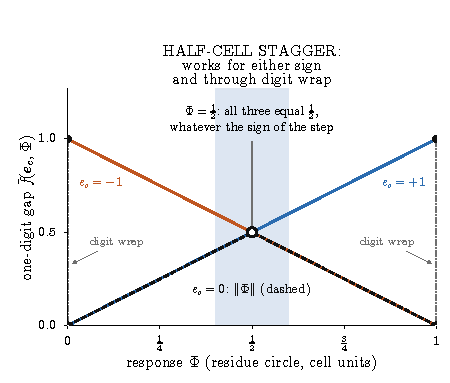
\includegraphics[width=0.48\linewidth]{fig_halfcell_v4.pdf}
\caption{The half-cell stagger: the one-digit gap $\bar f(e,\Phi)$ of Lemma~\ref{lem:antipode} for $e=+1,-1,0$. $\Phi=\frac12$ is the only response where all three agree, whatever the sign of the step; a window $\frac12\pm0.1$ is shaded (schematic).}
\label{fig:principles}
\end{figure}

\begin{figure}[t]
\centering
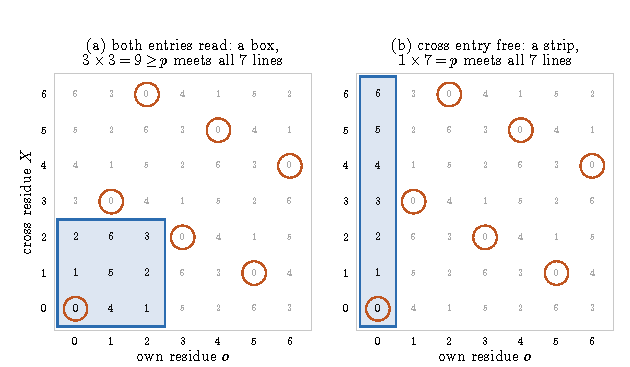
\includegraphics[width=0.66\linewidth]{fig_volume_v4.pdf}
\caption{The volume bound (Lemma~\ref{lem:volume}) for $s=2$, $p=7$, $\alpha=(1,3)$. The free digit of column $c'$ moves its responses along a line $\beta+\F_p\alpha_{c'}$, so the column window must meet every line; each pair (own, cross) is labelled by its line. (a)~A $3\times3$ box meets all $7$ lines. (b)~A strip with one own value and the full cross axis also meets all $7$ lines; an entry that the bound never reads costs nothing. Both coverings are checked exhaustively.}
\label{fig:cost}
\end{figure}

\subsection{Staggered Windows at a Finite Prime}\label{app:BSfinite}
This subsection proves Theorem~\ref{thm:A}: the bound for staggered windows at a finite prime (Lemma~\ref{lem:W}), the realization of the depth-zero crosses with the half from a power of two (Lemmas~\ref{lem:D} and~\ref{lem:R}), the staggered rule (Definition~\ref{def:BS}) and its thresholds (Proposition~\ref{prop:P0}, Theorem~\ref{thm:A3}). Throughout, $p$ is an odd prime and $C=\{c\ne\cstar\}$.

At a finite prime the windows of Section~\ref{sec:staggered} become integer intervals. We use three half-widths in row$\leftarrow$column order: $B_{C\leftarrow C}$ (into a coordinate of $C$ from another one), $B_{\star\leftarrow C}$ (the half-cell offsets) and $B_{C\leftarrow\star}$ (into $C$ from $\cstar$). For integers $A\ge0$, $M_i\ge1$ ($i\in C$) and $M_\star\ge1$, with $M:=\max_iM_i$, the \emph{staggered windows at $p$} are: in column $i\in C$, own $[-(A+M_i-1),-A]$, $W_{\star\leftarrow i}=\half+[-B_{\star\leftarrow C},B_{\star\leftarrow C}]$, $W_{j\leftarrow i}=[-B_{C\leftarrow C},B_{C\leftarrow C}]$ for $j\in C\setminus\{i\}$; in column $\cstar$, own $[-(M_\star-1),0]$ and $W_{j\leftarrow\star}=[-B_{C\leftarrow\star},B_{C\leftarrow\star}]$ for $j\in C$.

\begin{lemma}[Bound for staggered windows]\label{lem:W}
Let $s\ge2$ and suppose
\[
\text{(D)}\ A\ge(s-2)B_{C\leftarrow C}+B_{C\leftarrow\star},\qquad\text{(N)}\ A+M+(s-2)B_{C\leftarrow C}+B_{C\leftarrow\star}\le p,\quad 2B_{\star\leftarrow C}+2M_\star\le p-3 .
\]
Then $\LB(W)\ge\LB_W$, where $\LB_W^2=\min(T_\star,T_{C\star},T_2)$ with
\begin{align*}
T_\star&=\Bigl(1-\frac{M_\star}p\Bigr)^2,\qquad T_{C\star}=\Bigl(1-\frac{A+M+B_{C\leftarrow\star}}p\Bigr)^2+\Bigl(\frac{p-1-2B_{\star\leftarrow C}-2M_\star}{2p}\Bigr)^2,\\
T_2&=2\Bigl(1-\frac{A+M+(s-2)B_{C\leftarrow C}+B_{C\leftarrow\star}}p\Bigr)^2\quad(\text{omitted for }s=2).
\end{align*}
In particular, with $x:=1-((s-2)B_{C\leftarrow C}+2B_{C\leftarrow\star})/p$, $y:=\frac12-B_{\star\leftarrow C}/p$ and $A=(s-2)B_{C\leftarrow C}+B_{C\leftarrow\star}$: if $x\ge M/p$, $p(x^2+y^2-1)\ge2xM+2y(M_\star+\frac12)$ and $1-(2A+M)/p\ge1/\sqrt2$, then $\LB_W=1-M_\star/p$.
\end{lemma}

\begin{proof}
By Remark~\ref{rem:onedigit}, $f_1(1,-a)=1-(a+1)/p$ for $0\le a<p$, $f_1(1,\sigma)=(\sigma-1)/p$ for $\sigma\in[1,p-1]$, $f_1(-1,\sigma)=f_1(1,-\sigma)$, and $f_1(0,\sigma)=\max(0,\cabs\sigma-1)/p$. Fix a step $e$, $E=\operatorname{supp}e$, $k=|E\cap C|$. A moving coordinate $i\in C$ receives its own response and one cross from each other moving column, so by (D) and (N) $e_i\sigma_i\in[-(A+M-1)-(s-2)B_{C\leftarrow C}-B_{C\leftarrow\star},\,0]\subseteq[-(p-1),0]$, and $f_1(e_i,\sigma_i)\ge1-(A+M+(s-2)B_{C\leftarrow C}+B_{C\leftarrow\star})/p$; if besides $i$ only $\cstar$ moves, this improves to $1-(A+M+B_{C\leftarrow\star})/p$, and if $i$ moves alone to $1-(A+M)/p$. If $k\ge2$, two such coordinates give $T_2$. If $E=\{\cstar\}$, $f_1(1,O_\star)\ge1-M_\star/p$, which is $T_\star$. If $E=\{i\}$, the staggered coordinate does not move and receives $\half+\xi$ with $|\xi|\le B_{\star\leftarrow C}$, of centred absolute value at least $(p-1)/2-B_{\star\leftarrow C}$; the term is at least $(1-(A+M)/p)^2+((p-3-2B_{\star\leftarrow C})/(2p))^2\ge T_{C\star}$. If $E=\{i,\cstar\}$, then $e_\star\sigma_\star=\pm(\half+\xi)+O_\star$ is an integer in $[(p-1)/2-B_{\star\leftarrow C}-M_\star+1,\,(p+1)/2+B_{\star\leftarrow C}]\subseteq[1,p-1]$ by (N), so $f_1\ge(p-1-2B_{\star\leftarrow C}-2M_\star)/(2p)$, and with coordinate $i$ this is $T_{C\star}$. For the last statement, $1-(A+M+B_{C\leftarrow\star})/p=x-M/p$ and the second base of $T_{C\star}$ is at least $y-(M_\star+\frac12)/p$; since $(x-\eta_1)^2+(y-\eta_2)^2\ge x^2+y^2-2x\eta_1-2y\eta_2$, the hypothesis gives $T_{C\star}\ge1$, and $T_2\ge1$ directly.
\end{proof}

The lemma is Theorem~\ref{thm:BS} at finite $p$: with half-widths about $\varepsilon p$ and $A=(s-1)B$ its bases tend to $1-s\varepsilon$, $\frac12-\varepsilon$ and $1-2(s-1)\varepsilon$, and $x^2+y^2>1$ holds for $\varepsilon<\varepsilon_s$. Under the last statement the only loss of order $1/p$ is the own window of $\cstar$.

\emph{Realising the windows.} The fixed depth-zero crosses must lie in the windows (condition (i) of Proposition~\ref{prop:steer}): the half-cell offsets $-\kappa_{\star\leftarrow i}$ near $\half$ and all others within $O(p)$ of $0$; and every column must cover (condition (ii)). A cross $\kappa\equiv x/2$ with a small odd integer $x$ is close to $p/2$, and its multiples alternate between the two half-circles, so no mixed-radix hierarchy sees it as a small step. Its double is the small odd number $x$, and doubling the column costs a factor $2$ in the own window and nothing else.

\begin{lemma}[Doubling]\label{lem:D}
Let $\boldsymbol\xi\in\F_p^k$, let $\mathbf m\in\Z^k$ represent $2\boldsymbol\xi$, and suppose that $\mathbf m$ satisfies the hypotheses of Lemma~\ref{lem:ws} for arcs $I_1,\dots,I_k$, with number $N_k$. If $\Wo$ contains $2N_k-1$ consecutive integers, then for every $\sigma\in\F_p^k$ some $o\in\Wo$ has $\sigma+o\,\boldsymbol\xi\in I_1\times\dots\times I_k$.
\end{lemma}

\begin{proof}
$\Wo$ contains $o_0,o_0+2,\dots,o_0+2(N_k-1)$, and $\sigma+(o_0+2o')\boldsymbol\xi=(\sigma+o_0\boldsymbol\xi)+o'\mathbf m$ for $o'=0,\dots,N_k-1$; Lemma~\ref{lem:ws} applies to $\sigma+o_0\boldsymbol\xi$.
\end{proof}

By the computation at the start of Appendix~\ref{app:coverings}, this is condition (ii) for a column with steps $\boldsymbol\xi=(\kappa_{c\leftarrow c'})_{c\ne c'}$; we call such a column a \emph{doubled column}. The half itself comes from the $2$-adic valuation of the scale. By Proposition~\ref{prop:LI}(c), with the constant terms $g_c=g_c(0)$ of the multipliers,
\[
\kappa_{c\leftarrow c'}=\frac{\theta\,g_c}{g_{c'}\,\Delta_{cc'}},\qquad \Delta_{cc'}:=w'(a_{c'})\,(a_{c'}-a_c).
\]
\emph{Staggered data} $\mathcal D$ consist of distinct rational places $a_0,\dots,a_{s-1}$, a staggered coordinate $\cstar$, an order $j_1,\dots,j_{s-1}$ of $C$, and positive rationals $Q_1,\dots,Q_{s-1}$ with odd numerators and odd denominators. Let $\delta\ge0$ be the least integer with $1+2\delta\ge v_2(\Delta_{j_t\star}\Delta_{\star j_t})$ and $\delta+v_2(\Delta_{\star j_r})-v_2(\Delta_{\star j_t})-v_2(\Delta_{j_tj_r})\ge0$ for all $t\ne r$, where $v_2$ is the $2$-adic valuation, and let $L$ be the least odd positive integer such that every $L/Q_r$ and every $L\,n^\circ_{cc'}$, $c\ne\cstar$, is an integer, where $n^\circ_{cc'}$ is the value of the rational $n_{cc'}$ below at $L=1$ (it exists by the choice of $\delta$).

\begin{lemma}[The half from a power of two]\label{lem:R}
For staggered data put $g_{\cstar}=1$, $g_{j_r}=2^{1+\delta}Q_r/\Delta_{\star j_r}$ and $\theta=2^\delta LT$ with an odd integer $T$. Then $\kappa_{c\leftarrow c'}=T\,n_{cc'}$ with
\[
n_{j_t\leftarrow\star}=\frac{2^{1+2\delta}LQ_t}{\Delta_{j_t\star}\Delta_{\star j_t}}\in\Z,\qquad n_{j_t\leftarrow j_r}=2^\delta L\,\frac{Q_t}{Q_r}\cdot\frac{\Delta_{\star j_r}}{\Delta_{\star j_t}\Delta_{j_tj_r}}\in\Z,\qquad n_{\star\leftarrow j_r}=\frac{L}{2Q_r}\in\tfrac12+\Z .
\]
For every prime $p$ that divides none of the numerators and denominators of the $a_c-a_{c'}$, the $Q_r$, $L$, $T$ and $2$, the same identities hold in $\F_p$; there every $\kappa_{c\leftarrow c'}$ with $c\ne\cstar$ is the integer $Tn_{cc'}$, and each half-cell offset is $\kappa_{\star\leftarrow j_r}\equiv\half+(TL/Q_r-1)/2$, half a cell plus an integer.
\end{lemma}

\begin{proof}
Substitute $g$ and $\theta$. In the row of $\cstar$ the frame factor cancels,
\[
\frac{\theta}{g_{j_r}\Delta_{\star j_r}}=\frac{2^\delta LT}{2^{1+\delta}Q_r}=\frac{TL}{2Q_r},
\]
and $L/Q_r$ is an odd integer. The other two expressions are integers by the choice of $L$, which is possible because their $2$-adic valuations are $1+2\delta-v_2(\Delta_{j_t\star}\Delta_{\star j_t})\ge0$ and $\delta+v_2(\Delta_{\star j_r})-v_2(\Delta_{\star j_t})-v_2(\Delta_{j_tj_r})\ge0$. Modulo $p$, a half-odd rational $x/2$ is $(x+p)/2=\half+(x-1)/2$.
\end{proof}

So the half needs no congruence condition on $p$ and no root of unity, and all crosses are fixed rational multiples of one odd integer $T$.

\begin{definition}[Staggered rule]\label{def:BS}
Let $\mathcal D$ be staggered data, $\varepsilon_{C\leftarrow\star},\varepsilon_{C\leftarrow C},\varepsilon_{\star\leftarrow C}$ positive rationals (window fractions) and $u>0$ rational. At a prime $p$ as in Lemma~\ref{lem:R} with $up\ge1$:
(S1)~$T$ is the largest odd integer $\le\lfloor up\rfloor$; $\theta$ and the constants $g_c$ are those of Lemma~\ref{lem:R}, so $\kappa_{c\leftarrow c'}=Tn_{cc'}$;
(S2)~$B_\bullet=\lfloor\varepsilon_\bullet p\rfloor$ for the three half-widths, $A=(s-2)B_{C\leftarrow C}+B_{C\leftarrow\star}$, and the windows of Lemma~\ref{lem:W};
(S3)~$M_\star$ is the number $N_{s-1}$ of Lemma~\ref{lem:ws} for column $\cstar$ (steps $|\kappa_{j\leftarrow\star}|$ in decreasing order, arcs $[-B_{C\leftarrow\star},B_{C\leftarrow\star}]$), and $M_i=2N^{(i)}-1$, where $N^{(i)}$ is the number of Lemma~\ref{lem:ws} for the doubled column $i$ (steps $|2\kappa_{c\leftarrow i}|$ in decreasing order, the half-cell offset contributing the odd integer $|TL/Q_r|$; arcs of the rows);
(S4)~any selection rule (Appendix~\ref{app:steerrule}).
\end{definition}

The rule is a fixed computation of $O(s^2)$ integer operations plus the selection of the free digits; it involves no search and no covering check. It satisfies the hypotheses of Proposition~\ref{prop:steer} and Lemmas~\ref{lem:ws}, \ref{lem:D} and~\ref{lem:W} for all large $p$ as soon as its limit as $p\to\infty$ does. For a column, let $\bar\nu_1\ge\dots\ge\bar\nu_{s-1}>0$ be its steps divided by $p$ in the limit, $\bar\nu=u|n_{c\leftarrow\star}|$ in column $\cstar$ and $\bar\nu=2u|n_{c\leftarrow i}|$ in a doubled column $i\in C$, and let $\lambda_t=2\varepsilon_\bullet$ be the window fraction of the corresponding row. The data satisfy the \emph{limit hierarchy} if in every column
\[
\bar\nu_1<\lambda_1,\qquad \bar N_{t-1}\,\bar\nu_t<\lambda_t\quad(2\le t\le s-1),\qquad \bar N_1=2+\frac{1-\lambda_1}{\bar\nu_1},\quad \bar N_t=\bar N_{t-1}+\frac1{\bar\nu_t},
\]
and the fixed depth-zero crosses lie strictly inside their windows: $u|n_{c\leftarrow c'}|<\varepsilon_\bullet$ for $c\ne\cstar$ and $2u|n_{\star\leftarrow i}|<2\varepsilon_{\star\leftarrow C}$. These are the limits of the hypotheses of Lemma~\ref{lem:ws} and of condition (i).

\begin{proposition}[Threshold]\label{prop:P0}
For the staggered rule with given data there are an explicit finite conjunction $\mathcal P(p)$ of inequalities between rational functions of a real variable $p$ and an explicit function $M_\star^+(p)$ such that (a) and (b) hold; if moreover the data satisfy the limit hierarchy, $0<\varepsilon_{\star\leftarrow C}<\frac12$, and $x=1-(s-2)\varepsilon_{C\leftarrow C}-2\varepsilon_{C\leftarrow\star}$ and $y=\frac12-\varepsilon_{\star\leftarrow C}$ satisfy $x^2+y^2>1$ and $1-2(s-2)\varepsilon_{C\leftarrow C}-2\varepsilon_{C\leftarrow\star}>1/\sqrt2$, then also (c) holds.
\begin{enumerate}
\item[(a)] At every prime $p$ as in Lemma~\ref{lem:R} with $\mathcal P(p)$, the staggered rule satisfies (i) and (ii) of Proposition~\ref{prop:steer} and the hypotheses of Lemma~\ref{lem:W} including its last statement, with $M_\star\le M_\star^+(p)$.
\item[(b)] $\mathcal P(p)$ implies $\mathcal P(p')$ for every $p'\ge p$, and $M_\star^+$ is non-increasing.
\item[(c)] $\mathcal P(p)$ holds for all large $p$.
\end{enumerate}
Consequently, if $\mathcal P(p_0)$ holds, then for every prime $p\ge p_0$ as in Lemma~\ref{lem:R} the staggered rule gives a digital $(0,s)$-sequence over $\F_p$ with $\sep{P_{sK}}\ge1-C''/p$ for every $K$, where $C'':=M_\star^+(p_0)$; under the hypotheses of (c) such a $p_0$ exists.
\end{proposition}

The list $\mathcal P$ and the proof are in Appendix~\ref{app:windowdata}; any $p_0$ with $\mathcal P(p_0)$ is a valid threshold, certified by one exact rational evaluation.

\begin{theorem}[The staggered rule in dimension three]\label{thm:A3}
Let $s=3$ and take the staggered data with the Faure places $(0,1,2)$, $\cstar=0$, order $(1,2)$ and $(Q_1,Q_2)=(7,3)$; then $\delta=2$, $L=21$, $\theta=84T$, $g=(1,-56,6)$, and
\[
\kappa_{1\leftarrow0}=2352T,\quad\kappa_{2\leftarrow0}=-126T,\quad\kappa_{0\leftarrow1}=\tfrac32T,\quad\kappa_{0\leftarrow2}=\tfrac72T,\quad\kappa_{1\leftarrow2}=-392T,\quad\kappa_{2\leftarrow1}=-9T.
\]
With $u=891/78\,400\,000$ and $(\varepsilon_{C\leftarrow\star},\varepsilon_{C\leftarrow C},\varepsilon_{\star\leftarrow C})=(\frac{27}{1000},\frac1{200},\frac1{10})$, the staggered rule gives for every prime $p\ge1.97\cdot10^7$ a quasi-uniform digital $(0,3)$-sequence over $\F_p$ with $\sep{P_{3K}}\ge1-742/p$ for every $K\ge1$.
\end{theorem}

\begin{proof}
The six crosses are Lemma~\ref{lem:R} (the excluded primes are $2$, $3$, $7$). The condition $\mathcal P(p_0)$ holds at $p_0=19\,673\,600$, with $M_\star^+(p_0)=742.355\ldots$, by one exact rational evaluation (proof${}^\star$); as $M_\star$ is an integer, $M_\star\le742$. Lemma~\ref{lem:prefix} gives quasi-uniformity.
\end{proof}

The half-cell offsets are $\frac32T$ and $\frac72T$; in column $\cstar$ the fast row has the step $\kappa_{1\leftarrow0}\approx0.027p$; the first-order deficit $742$ is the size of the own window of $\cstar$.

\begin{remark}[Below the threshold]\label{rem:A3range}
The hypotheses of Proposition~\ref{prop:steer} and Lemma~\ref{lem:W} for this rule are integer conditions at each prime. Checked at all $1\,035\,877$ primes in $[3\cdot10^6,1.97\cdot10^7]$ by a program that computes the crosses in $\F_p$ from the constants $g_c$ (not from Lemma~\ref{lem:R}), they hold with $(1-\LB_W)p\le779$ (c.a.). So the staggered rule gives $\sep{P_{3K}}\ge1-779/p$ for every prime $p\ge3\cdot10^6$.
\end{remark}

\begin{proof}[Proof of Theorem~\ref{thm:A}]
Take any staggered coordinate, the natural order of $C$, uniform window fractions $\varepsilon<\varepsilon_s$, and $Q_r=R^r$ with an odd integer $R$. By Lemma~\ref{lem:R}, $n_{cc'}=2^\delta L\,R^{e}f_{cc'}$, where $f_{cc'}$ does not depend on $R$ and $e=t$ in row $j_t$ of column $\cstar$, $e=t-r$ in row $j_t$ of column $j_r$, and $e=-r$ for the half-cell offset of column $j_r$. The exponents in one column are distinct, so for $R$ large consecutive steps of every column differ by a factor at least $1+1/\varepsilon$, and the largest step of every column $i\in C$ (exponent at most $s-2$) is smaller than the largest step of column $\cstar$ (exponent $s-1$). Choose $u$ so that the latter is $(1-\eta)\varepsilon$ with $0<\eta<1$. Then $\bar\nu_1<\lambda_1=2\varepsilon$ in every column, the fixed depth-zero crosses are strictly inside their windows, and for $t\ge2$
\[
\bar N_{t-1}\bar\nu_t\le2\bar\nu_t+\sum_{r<t}\frac{\bar\nu_t}{\bar\nu_r}\le2\bar\nu_t+\sum_{j\ge1}\Bigl(1+\frac1\varepsilon\Bigr)^{-j}=2\bar\nu_t+\varepsilon<2\varepsilon=\lambda_t,
\]
because $2\bar\nu_t\le4\varepsilon/(1+1/\varepsilon)<\varepsilon$ for $\varepsilon<\frac13$. So the limit hierarchy holds. With uniform widths, $x=1-s\varepsilon$ and $y=\frac12-\varepsilon$, and $x^2+y^2>1$ follows from $\varepsilon<\varepsilon_s$ (proof of Theorem~\ref{thm:BS}); as $y^2<\frac14$, this forces $(1-s\varepsilon)^2>\frac34$, hence $1-2(s-1)\varepsilon>1-(2-\sqrt3)>1/\sqrt2$. Proposition~\ref{prop:P0} gives $p_0(s)$ and $C''_s$; the primes excluded in Lemma~\ref{lem:R} are finitely many, and Lemma~\ref{lem:prefix} gives quasi-uniformity.
\end{proof}

For $s=4$ (staggered coordinate $0$, $R=153$, $\varepsilon=7/250$) Proposition~\ref{prop:P0} gives $p_0=1.44\cdot10^{16}$ and $C''_4=32\,044$, and for $s=5$ (staggered coordinate $4$, $R=99$, $\varepsilon=23/1000$) $p_0=1.98\cdot10^{21}$ and $C''_5=2.73\cdot10^9$ (exact rational evaluations, proof${}^\star$; Table~\ref{tab:BSdata}). Coverings of lattice type instead of one shared hierarchy of step sizes are a possible route to lower thresholds (Section~\ref{sec:open}). Figure~\ref{fig:bsgeom} shows the geometry of Section~\ref{sec:staggered} in a staggered window system at a moderate prime, with coverings checked exactly instead of by the rule.

\begin{figure}[t]
\centering
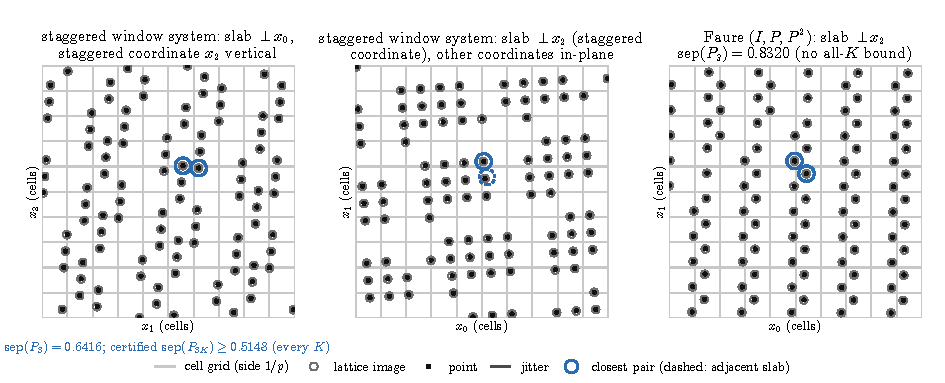
\includegraphics[width=\linewidth]{fig_bs_slab_v4.pdf}\\[2pt]
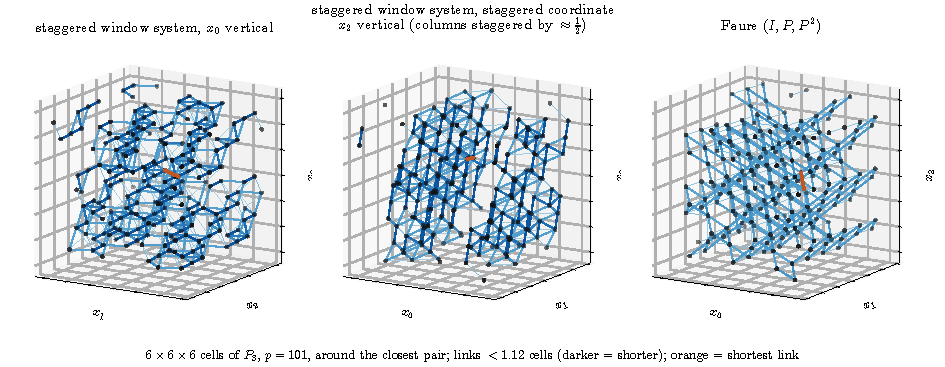
\includegraphics[width=\linewidth]{fig_bs_3d_v4.pdf}
\caption{Staggered windows in dimension three: a staggered window system at $p=101$ with exactly checked coverings (certified $\sep{P_{3K}}\ge0.5148$ for every $K$) and one admissible choice of the free digits. Top: slabs of $P_3$ one cell thick, $10\times10$ cells around the closest pair. Left, staggered coordinate vertical: the columns are staggered by about half a cell. Middle, orthogonal to the staggered coordinate: the coordinates of $C$ are pushed together and wrap around along staircases. Right, Faure $(I,\Pas,\Pas^2)$. Exact $\sep{P_3}$: $0.6416$, and $0.8320$ for Faure, which has no bound for all levels. Bottom: $6\times6\times6$ cells around the closest pair, links shorter than $1.12$ cells (darker $=$ shorter, orange $=$ shortest), in the same three views.} %
\label{fig:bsgeom}
\end{figure}

\subsection{Staggered Data and Thresholds}\label{app:windowdata}
\emph{Staggered data.} Table~\ref{tab:BSdata} gives the three staggered rules of Theorems~\ref{thm:A3} and~\ref{thm:A}. In each, $\theta=2^\delta LT$ and $\kappa_{c\leftarrow c'}=Tn_{cc'}$ with the rationals $n_{cc'}$ of Lemma~\ref{lem:R}; for $s=4,5$ the window fractions are uniform, $\varepsilon_{C\leftarrow\star}=\varepsilon_{C\leftarrow C}=\varepsilon_{\star\leftarrow C}=\varepsilon$, with $u=\frac{999}{1000}\,\varepsilon/\max_t|n_{j_t\leftarrow\star}|$, which puts the step of the fast row of column $\cstar$ just inside its window.

\begin{table}[t]
\centering
\small
\caption{The staggered data: Faure places $(0,1,\dots,s-1)$, staggered coordinate $\cstar$, order of $C$, the rationals $Q_r$, the $2$-adic data $\delta$, $L$ and the constants $g_c$ of Lemma~\ref{lem:R} (for $c=0,\dots,s-1$), window fractions, $u$, the threshold $p_0$ (exact bisection endpoint, rounded up in the last digit shown) and the first-order deficit $C''=M_\star^+(p_0)$ (rounded up).}
\label{tab:BSdata}
\begin{tabular}{@{}lccc@{}}
\toprule
& $s=3$ (Thm.~\ref{thm:A3}) & $s=4$ & $s=5$\\
\midrule
$\cstar$; order & $0$; $(1,2)$ & $0$; $(1,2,3)$ & $4$; $(0,1,2,3)$\\
$Q_r$ & $(7,3)$ & $153^r$ & $99^r$\\
$\delta$; $L$ & $2$; $21$ & $2$; $3\,581\,577$ & $5$; $96\,059\,601$\\
$g_c$ & $(1,-56,6)$ & $(1,612,-46818,1591812)$ & $(-66,34848,-7762392,$\\
& & & $1024635744,1)$\\
$(\varepsilon_{C\leftarrow\star},\varepsilon_{C\leftarrow C},\varepsilon_{\star\leftarrow C})$ & $(\frac{27}{1000},\frac1{200},\frac1{10})$ & $\varepsilon=\frac7{250}$ & $\varepsilon=\frac{23}{1000}$\\
$u$ & $891/78\,400\,000$ & $259/(1.1730858534\cdot10^{16})$ & $851/(4.860548184640896\cdot10^{21})$\\
$p_0$ & $19\,673\,600$ & $1.43146\cdot10^{16}$ & $1.97832\cdot10^{21}$\\
$C''$ & $742.356$ & $32044.14$ & $2.72224\cdot10^9$\\
\bottomrule
\end{tabular}
\end{table}

\emph{The predicate $\mathcal P(p)$.} Fix staggered data and a real $p>0$. For a column, sort its steps by $|n|$ in decreasing order, $n_1,\dots,n_{s-1}$; let $k=1$ for column $\cstar$ and $k=2$ for a column $i\in C$ (Lemma~\ref{lem:D}; there the half-cell offset contributes $2|n_{\star\leftarrow i}|=L/Q_r$), and let $\lambda_t=2\varepsilon_\bullet$ be the window fraction of the row of step $t$. Put
\[
\nu_t^-=k|n_t|(up-2),\qquad\nu_t^+=k|n_t|\,up,\]\[N_1^+=2+\max\Bigl(0,\frac{p-(p\lambda_1-1)}{\nu_1^-}\Bigr),\qquad N_t^+=N_{t-1}^++\frac p{\nu_t^-},
\]
let $M_\star^+$ be $N_{s-1}^+$ of column $\cstar$ and $M^+$ the maximum of $2N_{s-1}^+-1$ over the columns $i\in C$, and let $x$, $y$ be as in Proposition~\ref{prop:P0}. Then $\mathcal P(p)$ is the conjunction of
(P1)~$up>2$;
(P2)~in every column, $\nu_1^+\le p\lambda_1-1$ and $N_{t-1}^+\nu_t^+\le p\lambda_t-1$ for $2\le t\le s-1$;
(P3)~$|n_{c\leftarrow c'}|\,up\le\varepsilon_\bullet p-1$ for every cross with $c\ne\cstar$, where $\varepsilon_\bullet$ is the fraction of its window, and $|2n_{\star\leftarrow i}|\,up\le2(\varepsilon_{\star\leftarrow C}p-1)-1$ for every half-cell offset;
(P4)~$x^2+y^2>1$ and $p\,(x^2+y^2-1)\ge2xM^++2y\,(M_\star^++\frac12)$;
(P5)~$z:=1-2(s-2)\varepsilon_{C\leftarrow C}-2\varepsilon_{C\leftarrow\star}-M^+/p\ge0$ and $2z^2\ge1$;
(P6)~$\bigl(2(s-2)\varepsilon_{C\leftarrow C}+2\varepsilon_{C\leftarrow\star}\bigr)p+M^++2\le p-1$, $2\varepsilon_{\star\leftarrow C}\,p+2M_\star^++2<p-1$ and $x>M^+/p$.
At a prime $p$, $T\in(up-2,up]$ and every arc of row $t$ has at least $p\lambda_t-1$ elements, so (P2) gives the hypotheses of Lemma~\ref{lem:ws} (with $N_t\le N_t^+$), (P3) condition (i) of Proposition~\ref{prop:steer}, and (P4)--(P6) the hypotheses of Lemma~\ref{lem:W} including its last statement ((P5) is $z\ge1/\sqrt2$; under (P6) the difference of the two sides of $p(x^2+y^2-1)\ge2xM+2y(M_\star+\frac12)$ increases in $x$ and $y$).

\begin{proof}[Proof of Proposition~\ref{prop:P0}]
$\mathcal P$ is obtained from the hypotheses by four substitutions: $T\in(up-2,up]$, so every step lies in $[k|n|(up-2),\,k|n|up]$; every arc has at least $p\lambda_t-1$ elements; $\lceil z\rceil\le z+1$ in the recursion of Lemma~\ref{lem:ws}, which bounds the numbers $N_t$ by the sums $N_t^+$, and hence $M_\star$, $M$ by $M_\star^+$, $M^+$; and Lemma~\ref{lem:W} is replaced by its last statement. Since $T$ is common to all entries, sorting the steps of a column by size is sorting by $|n|$, independently of $p$. (a) is the statement that each substituted inequality implies the original one; for the half-cell offsets, $2\kappa_{\star\leftarrow i}=TL/Q_r$ is an odd integer and $-\kappa_{\star\leftarrow i}\equiv\half-(TL/Q_r+1)/2$. (b) Each $N_t^+$ is a sum of terms that decrease in $p$ for $up>2$, and after division by $p$ every inequality of $\mathcal P$ has the form ``non-increasing $\le$ non-decreasing''. (c) The hypotheses give $\varepsilon_{\star\leftarrow C}<\frac12$ and $2(s-2)\varepsilon_{C\leftarrow C}+2\varepsilon_{C\leftarrow\star}<1$, so every window fraction is below $\frac12$, $\lambda_1<1$ and the maximum in $N_1^+$ is its second term. As $p\to\infty$, $N_t^+\to\bar N_t$ and $M^+/p\to0$, so the strict inequalities of the limit hierarchy give $\mathcal P(p)$ for large $p$. The bound is Proposition~\ref{prop:steer} with Lemma~\ref{lem:W}: $\LB(W)\ge1-M_\star/p\ge1-M_\star^+(p_0)/p$.
\end{proof}

By Proposition~\ref{prop:P0}(b), $\mathcal P$ is monotone, and a bisection in exact rational arithmetic gives a point $p_0$ where $\mathcal P(p_0)$ holds: $19\,673\,600$, $14\,314\,526\,192\,182\,751$ and $1\,978\,313\,734\,082\,584\,379\,393$ for $s=3,4,5$. Theorems~\ref{thm:A3} and~\ref{thm:A} round these up to $1.97\cdot10^7$, $1.44\cdot10^{16}$ and $1.98\cdot10^{21}$; since the own size $M_\star$ is an integer at most $M_\star^+(p_0)$, the first-order deficits are at most $742$, $32\,044$ and $2.73\cdot10^9$ (for $s=4$, $\mathcal P$ fails at $1.43\cdot10^{16}$).

\subsection{The Selection Rule}\label{app:steerrule}
For reproducibility we fix one deterministic choice of the free digits; the window sequences of the figures use it.

\begin{remark}[A greedy selection rule]\label{rem:steerrule}
In all our window systems the own windows are integer intervals $[\mathrm{lo}_c,\mathrm{hi}_c]\subseteq[-(p-1),0]$. Rank an admissible own value $o$ (its representative in the interval) by its distance $|2o-\mathrm{lo}_c-\mathrm{hi}_c|$ from the centre, ties to the larger $o$. At depth $1$ the responses are $D(1)$, with the own values on the diagonal and $-\kappa_{c\leftarrow c'}$ off it, and the admissible depth-one own values of different columns are independent. The rule chooses, over all combinations of admissible depth-one own values, one that maximises $\LBact_1$, ties broken by the ranking, column by column; at every depth $l\ge2$ it takes the best-ranked admissible own value of each column. It uses no look-ahead and no randomness, so a sequence is determined by its places, $\theta$, the $\lambda_c$ and the windows. By Proposition~\ref{prop:steer} it has the same bound $\min(1,\LB(W))$ at every full level as any other rule, and in addition $\sep{P_s}\ge\min(1,\LBact_1)$ with the best possible depth-one choice. That it maximises $\sep{P_s}$ or $\sep{P_{sK}}$ is not claimed; among the selection rules we compared on $\sep{P_3}$, it was within $10^{-3}$ of the best in $32$ of $35$ cases and never below $0.966$ of it, while rules that look at one column at a time lost up to $40\%$ at some primes.
\end{remark}


\bibliographystyle{amsplain}
\bibliography{refs}

\end{document}
